%\documentclass[onehalfspacing,oneside]{exeterthesis}
%\documentclass[a4paper,doublespacing,twoside,12pt]{exeterthesis}
\documentclass[a4paper,onehalfspacing,twoside,12pt,numbers=noenddot]{exeterthesis}


\usepackage{fontspec}
\setmainfont{Arial}
%% \setsansfont{Arial}
%% \setmainfont{Times New Roman}

\usepackage{tocloft}   % This package must be the first one
\usepackage{todo-book}

\usepackage{geometry}
% This has already set in the cls file
% \usepackage[a4paper, left=3cm, right=3cm, top=2cm, bottom=2cm]{geometry}
% \geometry{verbose,a4paper,textwidth=6.in,textheight=9.8in}
% \documentclass[twocolumn,journal]{IEEEtran}

\usepackage{amsmath}
\usepackage{amssymb}
\usepackage{graphicx}
% \usepackage{epstopdf}

\usepackage{fancyhdr}
%  \pagestyle{fancy}
%  \fancypagestyle{plain}{%
%     \fancyhf{} % clear all header and footer fields
%  
%     \lfoot[\thepage]{}
%     \rfoot[]{\thepage}
%     \renewcommand{\headrulewidth}{0pt}
%  }
%  %\fancypagestyle{fancy}{%
%     \fancyhf{}
%     %\renewcommand{\chaptermark}[1]{\markboth{\thechapter.\ #1}{}} 
%     \renewcommand{\chaptermark}[1]{\markboth{Chapter \thechapter.\ #1}{}} % Add Chapter by Qun Liu
%     \lhead{\leftmark}
%     %\rhead{\thepage}
%     \lfoot[\thepage]{}
%     \rfoot[]{\thepage}
%  %}

%%%% Qun Liu modify the header in April 20, 2018 %%%%
\fancyfoot{}
%\fancyhead{}
\renewcommand{\chaptermark}[1]{\markboth{Chapter \thechapter.\ #1}{}} 
\renewcommand{\sectionmark}[1]{\markright{\thesection.\ #1}} 
%\fancyhead[RO,LE]{\thepage}
%\fancyhead[LO]{\slshape\nouppercase \leftmark}
%\fancyhead[LO]{\nouppercase \leftmark}
%\fancyhead[RE]{\nouppercase \rightmark}
%%% E: Even page, O: Odd page, L: Left field, C: Center field, R: Right field, H: Header, F: Footer
\fancyhead[LE,RO]{\thepage}
\fancyhead[RE]{\nouppercase \leftmark}
\fancyhead[LO]{\nouppercase \rightmark}

%% -- One worked way to remove page number on the first page of chapter
%\makeatletter
%\let\ps@plain\ps@empty
%\makeatother
\fancypagestyle{plain}{ %
	\fancyhf{} % remove everything
	\renewcommand{\headrulewidth}{0pt} % remove lines as well
	\renewcommand{\footrulewidth}{0pt}
	\cfoot{\thepage} % Add page number at the center of page foot
}


%\usepackage{parskip}            % parskip separates non-indented paras by a blank line.
%\addtolength{\parskip}{0.2\parskip}

\usepackage{url}
%\usepackage{doublespace}

% --------------------- For reference ---------------------%
%\usepackage[square,sort]{natbib}
\usepackage[round]{natbib}
 %\usepackage[numbers]{natbib}
 
 % Try using biblatex, but failed... how to clean the aux file on overleaf
 % https://tex.stackexchange.com/questions/479736/overleaf-does-not-compile-after-using-biblatex
 % https://tex.stackexchange.com/questions/88195/is-there-an-biblatex-equivalent-to-natbibs-citealp-command
 % biblatex using .bbx rather than .bst for style file...
 %https://tex.stackexchange.com/questions/174676/how-to-use-custom-bibstyle-with-biblatex
 %\usepackage[style=authoryear,url=false,isbn=false,backref=true,sorting=ynt,natbib]{biblatex}
 % --------------------- For reference ---------------------%

\usepackage{float}
\usepackage[small,labelsep=space]{caption}
\setcapindent{0pt} % To stop the second and subsequent lines of captions being indented. (Caused by exeterthesis)

\usepackage{subfig}
\usepackage{mathtools}   % For \shortintertext

\usepackage{tikz}
\usetikzlibrary{arrows}
\usetikzlibrary{positioning}
\usetikzlibrary{fit}
\usetikzlibrary{decorations.pathreplacing}   % for curly brackets
\usetikzlibrary{shadows}

% Glossary
\usepackage{nomencl}
\makenomenclature
\renewcommand{\nomname}{Glossary}
\RequirePackage{ifthen}
\renewcommand{\nomgroup}[1]{%
   \ifthenelse{\not\equal{#1}{A}}{\vspace{5mm}}{}%
   \ifthenelse{\equal{#1}{A}}{\item[\textbf{Acronyms and abbreviations}]}{%
   \ifthenelse{\equal{#1}{B}}{\item[\textbf{Matrix/vector/scalar notation}]}{%
   \ifthenelse{\equal{#1}{C}}{\item[\textbf{Probability density functions}]}{%
   \ifthenelse{\equal{#1}{R}}{\item[\textbf{Roman}]}{%
   \ifthenelse{\equal{#1}{G}}{\item[\textbf{Greek}]}{}}}}}}

% Appendix
\usepackage{appendix}

\usepackage{fixltx2e}

%-------------------------------------------------------------------------------
% The following causes contents, citations, bookmarks etc to come out in colour.
%\usepackage[bookmarks=false]{hyperref}
%\hypersetup{linktoc=all,
%            unicode=true,
%            colorlinks=true,
%            pdfstartview=Fit,
%            pdfnewwindow=true}
%-------------------------------------------------------------------------------

\usepackage{scrhack}
\usepackage{lscape}

%\usepackage{framed}
\usepackage{afterpage}   % For \afterpage{\clearpage} to flush figures.
%\usepackage{fancybox}
%\setlength{\mylength}{\textwidth}%
%\newenvironment{FramedTable}%
%{\begin{table}[h]
%\begin{Sbox}%
%\setlength{\mylength}{\textwidth}%
%\addtolength{\mylength}{-2\fboxsep}%
%\addtolength{\mylength}{-2\fboxrule}%
%\begin{minipage}{\mylength}}%
%{\end{minipage}\end{Sbox}\fbox{\TheSbox}\end{table}}%


%\renewcommand{\topfraction}{0.9}	% max fraction of floats at top
%\renewcommand{\bottomfraction}{0.8}	% max fraction of floats at bottom
%   Parameters for TEXT pages (not float pages):
%    \setcounter{topnumber}{2}
%    \setcounter{bottomnumber}{2}
%    \setcounter{totalnumber}{4}     % 2 may work better
%    \setcounter{dbltopnumber}{2}    % for 2-column pages
%    \renewcommand{\dbltopfraction}{0.9}	% fit big float above 2-col. text
%    \renewcommand{\textfraction}{0.07}	% allow minimal text w. figs
%   Parameters for FLOAT pages (not text pages):
%\renewcommand{\floatpagefraction}{0.7}	% require fuller float pages
% N.B.: floatpagefraction MUST be less than topfraction !!
%\renewcommand{\dblfloatpagefraction}{0.7}	% require fuller float pages

% For thousands separators
\usepackage{siunitx}
%\usepackage[]{siunitx}

\usepackage{pifont}   % Also need to install the symbol package
\newcommand{\tick}{\ding{52}}

\usepackage{morefloats} % Latex Error: Float(s) lost.

%%%%%%%% ADDED BY MYSELF %%%%%%%%%%%
\usepackage{epigraph} % Added by Qun Liu, 2018/04/20, quoting
%\usepackage{fncychap}[Glenn]
%\usepackage[Glenn]{fncychap}
\usepackage{fncychap}  % Fancy chapter title styles
\usepackage{lipsum}  % Produce large text
\usepackage{bm} % math bold

\usepackage{booktabs} % for table, such as \midrule
\usepackage{multirow}
\usepackage{adjustbox}
\usepackage{diagbox}
\usepackage{mathrsfs}

%-------------------------------------------------------------------------------
% Qun Liu, self-defined commands, 24/Nov/2020
\newcommand{\secref}[1]{Section \ref{#1}}
\newcommand{\figref}[1]{Figure \ref{#1}}
\newcommand{\figsref}[1]{Figures \ref{#1}}
\newcommand{\tabref}[1]{Table \ref{#1}}
\newcommand{\Eqref}[1]{Equation (\ref{#1})}
\let\eqref\Eqref        % replace the original \eqref with \Eqref
\newcommand{\chapref}[1]{Chapter \ref{#1}}
%-------------------------------------------------------------------------------

\usepackage{rotating}
\usepackage{enumitem}


% % For biblatex, should import in the preamble
% \addbibresource{paperslib.bib}

%\includeonly{thesisPreamble}
%\includeonly{chapter1}
%\includeonly{chapter2}
%\includeonly{chapter3}
%\includeonly{chapter4}
%\includeonly{chapter5}
%\includeonly{appendix1}
%\includeonly{appendix2}

%-----------------------------
% 		Document title
%-----------------------------

%\title{My thesis title}
\title{Understanding climate feedbacks with idealized models}
%\title{Understanding cloud feedback with a simple cloud scheme}
%Understanding the cloud radiative effect response to climate change with a simple cloud scheme
\author{Qun Liu}
\date{July 2021}
\department{Mathematics}
%\supervisor{Prof. Matthew Collins and Prof. Geoffrey K. Vallis}
%\dedication{Some dedication text to thank various people.}
%\declaration{Declaration of work already published.}

%==============================
% 		Document body
%==============================
\begin{document}
% Uncomment these if you want to see your To-Do lists
%\listoftodos           % \todo{remember to do thins thing}
%\listoftodorefs        % \todoref{I need a reference for this}
%\listoftodoexps        % \todoexp{Do an experiment}

%% ============= Include the preamble ============= %%
% just comment for convenience
% thesisPreamble.tex

% \pagenumbering{roman}
% \clearpage
% %\pagenumbering{gobble}
\maketitle

%Abstract goes here.  Approx 300 words.
\begin{abstract}
%\addcontentsline{toc}{chapter}{Abstract}
This is part of abstract.
\end{abstract}

%% Declaration
\makedeclaration

%% Acknowledgements
%\makededication
\newpage
\chapter*{Acknowledgements}
%\addcontentsline{toc}{chapter}{Acknowledgements}
%% example
First and foremost, I would like to take this opportunity to thank my supervisors: Mat Collins and Geoff Vallis, for their generous guidance, support, motivation and endless patience. They always encourage me to...

I would like to acknowledge the joint PhD scholarship from University of Exeter and China Scholarship Council (NO. 201706210070), and I could not finish my PhD study without its support.

I am incredibly grateful to my family and friends for their continuous care and support over the last four years, especially during the Covid-19 lockdown period. Every week's video chat with my parents, brother and sometimes with my sister have gave me lots of support. My father Shugang and mother Hezhen, who are always there for me when I need any support, advice and help. My brother Yang, who has finished his PhD degree two years ago, sets a good example for me to follow. %, and who is always the first person I think of when I want to share some good or bad news.

%--------------------------------------------------------------
% List of contents
%--------------------------------------------------------------
\newpage
\pagestyle{fancy}
\setcounter{tocdepth}{4}
% Reset linkcolor to black
% https://tex.stackexchange.com/questions/59462/change-ref-color-of-on-the-list-of-figures
\bgroup
\hypersetup{linkcolor=black}
\tableofcontents
\egroup

%---------------------------------------------------------------
% List of tables, illustrations etc
%---------------------------------------------------------------
\newpage
\addcontentsline{toc}{chapter}{List of tables}
%\chapter*{List of tables}
\bgroup
\hypersetup{linkcolor=black}
\listoftables
\egroup

\newpage
\addcontentsline{toc}{chapter}{List of figures}
\bgroup
\hypersetup{linkcolor=black}
\listoffigures
\egroup
% Short caption in list of figures
% https://tex.stackexchange.com/questions/11579/short-captions-for-figures-in-listoffigures
% \caption[Short version for LoF]{Long version to appear next to the figure}

%--------------------------------------------------------------
% List of accompanying material (if any)
%--------------------------------------------------------------

%--------------------------------------------------------------
% Definitions (terms specific to the work); abbreviations
%--------------------------------------------------------------


% % Glossary
% % MakeIndex command line: makeindex thesis.nlo -s nomencl.ist -o thesis.nls
 \newpage
 \renewcommand{\nomname}{Nomenclature and Abbreviations}
 %\chapter*{Nomenclature and Abbreviations}
 \setlength{\nomlabelwidth}{2.5cm}
 \setlength{\nomitemsep}{-\parsep}
 % Acronyms
\nomenclature[aAMIP]{AMIP}{Atmospheric Model Intercomparison Project}
\nomenclature[aBOG]{BOG}{Byrne \& O'Gorman Radiation Scheme}
\nomenclature[aCMIP]{CMIP}{Coupled Model Intercomparison Project}
\nomenclature[aCRE]{CRE}{Cloud Radiative Effect}
\nomenclature[aCWP]{CWP}{Cloud Water Path}
\nomenclature[aEIS]{EIS}{Estimated Inversion Strength}
\nomenclature[aELF]{ELF}{Estimated Low-level Cloud Fraction}
\nomenclature[aGCM]{GCM}{General Circulation Model}
\nomenclature[aIPCC]{IPCC}{Intergovernmental Panel on Climate Change}
\nomenclature[aISCCP]{ISCCP}{International Satellite Cloud Climatology Project}
\nomenclature[aITCZ]{ITCZ}{Intertropical Convergence Zone}
\nomenclature[aPDF]{PDF}{Probability Density Function}
\nomenclature[aRRTM]{RRTM}{Rapid Radiative Transfer Model}
\nomenclature[aSOCRATES]{SOCRATES}{Suite of Community Radiation Codes based on Edwards \& Slingo Radiation Scheme}
\nomenclature[aSST]{SST}{Sea Surface Temperature}
\nomenclature[aSWLW]{SW, LW}{Shortwave, Longwave}
\nomenclature[aTOA]{TOA}{Top of the Atmosphere}

% Matrix, vector, scalar
%\nomenclature[ba]{$\bm X$}{A matrix.}
%\nomenclature[ba]{$z$}{A scalar.}
%\nomenclature[bb]{$\bm x_j$}{A column vector; the $j$th column of matrix $\bm X$; sometimes written as $\bm x_{:,j}$. There is one exception to this rule: the precision matrix $\bm B$ in chapter \ref{chap:2} retains its capitalisation to avoid confusion with other variables.}

% Roman letters
%\nomenclature[rT]{$T$}{The temperature.}

% Greek letters
\nomenclature[gl]{$\lambda$}{The climate feedback parameter}
\nomenclature[gw]{$\omega$}{Vertical pressure velocity}

% Greek alphabet ordering
% a alpha
% b beta
% c gamma
% d delta
% e epsilon
% f zeta
% g eta
% h theta
% i iota
% k kappa
% l lambda
% m mu
% n nu
% o xi
% p omicron
% q pi
% r rho
% s sigma
% t tau
% u upsilon
% v phi
% x chi
% y psi
% z omega

 \printnomenclature
 \addcontentsline{toc}{chapter}{Nomenclature and Abbreviations}
 \label{glossary}

%\clearpage
%% Begin new page of 
\pagestyle{fancy}
%\pagenumbering{arabic}

% \chapter{Introduction}
\label{ch:introduction}

\section{The Earth’s radiation budget}
The Earth's climate is driven by the energy flow into and out of the system. The incoming solar radiation (yellow fluxes in \figref{fig:earth_energy_budget}) reaches the Earth at the top of the atmosphere (TOA), then goes through the atmosphere and arrives at the Earth surface. During this process, approximately two thirds of this shortwave (SW) radiation is absorbed by the Earth surface and atmosphere, and roughly one third of this energy is reflected back to space. The the surface and atmosphere are heated by this incoming solar radiation, and they also re-emit the longwave (LW) radiation (purple fluxes in \figref{fig:earth_energy_budget}) to keep a relatively stable temperature. Globally, the annual mean incoming solar radiation flux is about 340 Wm$^{-2}$, the reflected solar radiation flux is around 100 Wm$^{-2}$ and the outgoing longwave radiation (OLR) is close to 240 Wm$^{-2}$ at the TOA for period 2000--2010 \citep{Stephens2012update}. These three components balance with each other, with a small positive imbalance (about 0.6 Wm$^{-2}$) at the TOA. A more recent estimate from \cite{Wild2015} (see their Fig. 1) indicates that the gloabl mean OLR is about 239 Wm$^{-2}$, and the TOA energy imbalance is about 1 Wm$^{-2}$.
%But due to the accuracy of the observation itself, it is hard to track the causes of these imbalance.

\begin{figure}[ht]
	\centering
	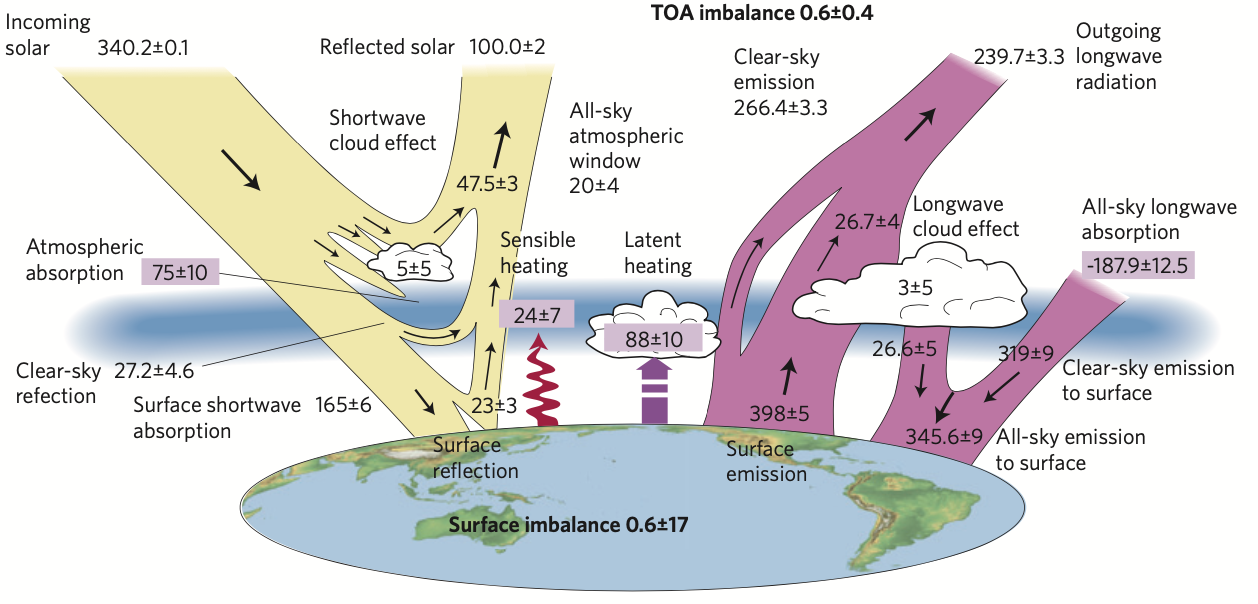
\includegraphics[width=1\linewidth]{{figs/literature_review/earth_enery_budget_Stephens2012}.png}
	\caption[The global annual mean energy budget of Earth for the approximate period 2000–2010 from \cite{Stephens2012update}]{The global annual mean energy budget of Earth for the approximate period 2000–2010. All fluxes are in Wm$^{-2}$. Solar fluxes are in yellow and infrared fluxes in purple. The four flux quantities in purple-shaded boxes represent the principal components of the atmospheric energy balance. Adapted from \cite{Stephens2012update}.}
	\label{fig:earth_energy_budget}
\end{figure}

As shown in \figref{fig:earth_energy_budget}, the energy budget at the Earth's surface is more complicated than at the TOA. When the incoming solar radiation reaches the surface, the majority (about 165 Wm$^{-2}$) of this solar radiation is absorbed by the surface and only a small portion (about 23 Wm$^{-2}$) is reflected back to space. Of course, these are global mean results and it would be different over certain areas such as Arctic where the surface albedo is large. The global annual mean LW radiation emitted from the surface is about 398 Wm$^{-2}$. Much of this is absorbed by the atmosphere (such as the greenhouse gases, aerosols and clouds), and only a small part (about 20 Wm$^{-2}$) can pass through the atmospheric window region (a portion of the infrared spectrum where there is almost no atmospheric absorption) reaching the TOA directly. The atmosphere can re-emit the absorbed LW radiation both upward and downward, and downward part (about 346 Wm$^{-2}$) can reheat the surface. In addition, due to the temperature and moisture difference between the surface and atmosphere, the surface is also cooled by the latent heat flux (about 88 Wm$^{-2}$) and sensible heat flux (about 24 Wm$^{-2}$) through the turbulent movement of atmosphere. In total, the surface energy budget is balanced by the downward/upward SW and LW radiation, the sensible and latent heat fluxes, but it has much larger uncertainty than at the TOA.

\section{Cloud radiative effect}

Clouds usually cover more than half areas of the Earth at any given time \citep{Houze2014,Ramanathan1989}, which is supported by recent International Satellite Cloud Climatology Project (ISCCP)\index{ISCCP} H-series products \citep{Young2018}, as shown in \tabref{tab:statistics_cld_amt}. Although they vary among different regions, the cloud amounts are usually larger over ocean regions than over lands, as the ocean provides a abundance of water vapor.

\begin{table}[htp]
\centering
%\scriptsize
\caption{Statistics of the annually averaged total cloud amount for various regions, which are from the ISCCP H-series data sets \citep{Young2018} from 1984 to 2014.}
\vspace{0.5em}
\begin{tabular}{cccc}
	\toprule
	Region & Ocean & Land &  Total\\
	\midrule
	Global & 71.7 & 54.8 & 66.1 \\
	15$^\circ$S--15$^\circ$N&  62.4&  63.5& 62.6 \\
	15$^\circ$N--35$^\circ$N&  60.1&  46.6& 55.2\\
	15$^\circ$S--35$^\circ$S&  65.0&  48.3& 61.4\\
	35$^\circ$N--60$^\circ$N&  80.9&  64.6& 72.5 \\
	35$^\circ$S--60$^\circ$S&  84.0&  65.0& 83.5 \\
	60$^\circ$N--90$^\circ$N&  68.9&  62.0& 66.5\\
	60$^\circ$S--90$^\circ$S&  80.1&  44.3& 60.1 \\
	\bottomrule
\end{tabular}
\label{tab:statistics_cld_amt}
\end{table}

\begin{figure}[ht]
	\centering
	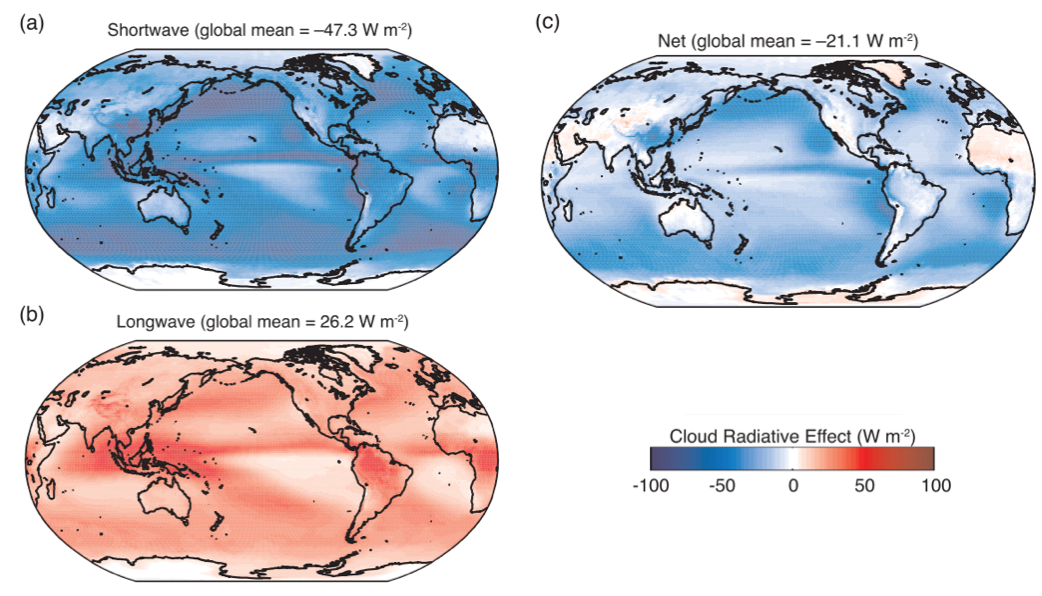
\includegraphics[width=1\linewidth]{{figs/literature_review/spatial_pattern_of_CRE_from_IPCC_ch7}.png}
	\caption{Distribution of annual-mean top of the atmosphere (a) shortwave, (b) longwave, (c) net cloud radiative effects averaged over the period 2001–2011 from the Clouds and the Earth’s Radiant Energy System (CERES) Energy Balanced and Filled (EBAF) Ed2.6r data set. Adapted from Fig. 7.7 of The Fifth Assessment Report (AR5) of the Intergovernmental Panel on Climate Change (IPCC) \citep{stocker2013climate}.}
	\label{fig:CRE_from_IPCC}
\end{figure}

\section{Cloud feedback}

\section{Cloud scheme}

\section{Research questions and thesis outline}
\label{sec:thesis_layout}

% %% literature_review_clouds.tex
\chapter{Backgrounds about Clouds and Cloud Schemes}
\label{ch:literature_review_about_clouds}

In the following chapters, we will focus on clouds and cloud scheme. To begin with, the literature about clouds and cloud schemes are reviewed in this chapter. A general introduction about clouds is presented in \secref{sec:cld_intro}. \secref{sec:cloud_feedback} focuses on cloud feedback and our current understandings about how cloud feedback changes in response to climate change. The coupling between clouds and circulation is briefly introduced in \secref{sec:cld_circulation_coupling}. A short history of cloud scheme development is reviewed in \secref{sec:cld_scheme_history}. In \secref{sec:why_simple_cld_schem_in_isca} what kind of simple cloud scheme will be implemented in Isca and the reasons to do so are presented.

%\section{Clouds in observatixons}
%What are clouds and the distribution of clouds from observations

%\epigraph{\textit{Let's begin the scientific journey!}}{\textit{Qun Liu}, 2018}
%\section{Clouds in the observations}

%\section{Roles of clouds in climate system}
%\label{sec:chp2_role_of_clouds}
% Literature review about the role of clouds in climate system

\section{Introduction}
\label{sec:cld_intro}
%\subsection{Introduction}
Clouds usually cover more than half areas of the Earth at any given time \citep{Houze2014,Ramanathan1989}, which is supported by recent International Satellite Cloud Climatology Project (ISCCP)\index{ISCCP} H-series products \citep{Young2018}, as shown in \tabref{tab:statistics_cld_amt}. Although they vary among different regions, the cloud amounts are usually larger over ocean regions than over lands, as the ocean provides a abundance of water vapor.

\begin{table}[htp]
\centering
%\scriptsize
\caption{Statistics of the annually averaged total cloud amount for various regions, which are from the ISCCP H-series data sets \citep{Young2018} from 1984 to 2014.}
\vspace{0.5em}
\begin{tabular}{cccc}
	\toprule
	Region & Ocean & Land &  Total\\
	\midrule
	Global & 71.7 & 54.8 & 66.1 \\
	15$^\circ$S-15$^\circ$N&  62.4&  63.5& 62.6 \\
	15$^\circ$N-35$^\circ$N&  60.1&  46.6& 55.2\\
	15$^\circ$S-35$^\circ$S&  65.0&  48.3& 61.4\\
	35$^\circ$N-60$^\circ$N&  80.9&  64.6& 72.5 \\
	35$^\circ$S-60$^\circ$S&  84.0&  65.0& 83.5 \\
	60$^\circ$N-90$^\circ$N&  68.9&  62.0& 66.5\\
	60$^\circ$S-90$^\circ$S&  80.1&  44.3& 60.1 \\
	\bottomrule
\end{tabular}
\label{tab:statistics_cld_amt}
\end{table}

Clouds play a fundamental role in Earth's radiation budget and hydrological cycle. In general, clouds can reflect the sunlight (shortwave radiation) back into space and absorb the longwave radiation emitted from the surface and cloud-free atmosphere, part of which will return to the surface. In general, the net effect of cloud is to cool the earth comparing to the cloud-free conditions. The net cooling effect of clouds is about 20 Wm$^{-2}$, which is roughly five times as large as the heating effect of doubling CO$_2$ \citep{Zelinka2017,Wild2019}. Small changes in clouds can have a large impact on the atmospheric energy balance due to balance between longwave and shortwave cloud effects. As a consequence, and not surprisingly, there are many studies focusing on the role of clouds in current climate or under climate change \citep[e.g.,][]{Cess1990intercomparison,Zelinka2017}.

% Therefore, even a small change of clouds could have large influence to the climate, that's one possible reason that why the cloud feedback is so important in climate system. 

%Clouds usually cover more than half areas of the Earth at any given time \citep{Houze2014} and play a fundamental role in Earth's radiation budget and hydrological cycle. In general, clouds can reflect the sunlight (shortwave radiation) back into space and absorb the longwave radiation emitted from the surface, part of which will return to the surface. In general, the net effect of cloud is to cool the earth comparing to the cloud-free conditions. According to \cite{Zelinka2017}, the net cooling effect of clouds is about 18 Wm$^{-2}$, which is roughly five times as large as the heating effect of doubling CO$_2$. Small changes in clouds can have a large impact on the climate energy balance due to balance between longwave and shortwave cloud effects. As a consequence, and not surprisingly, there are many studies focusing on the role of clouds under global warming \citep[e.g.,][]{Zelinka2017, Sherwood2020}.
% Therefore, even a small change of clouds could have large influence to the climate, that's one possible reason that why the cloud feedback is so important in climate system. 

%Besides interacting with radiation, clouds also couple with circulation \citep{Voigt2020review}.

Not only for the climatology, cloud responses to climate change have also attracted lots of attention. As described in detail in \secref{sec:cloud_feedback}, one important feature is cloud feedback, as it contributed a lot to the intermodel spread of the climate sensitivity of GCMs \citep{Ceppi2017, Sherwood2020}. In addition, clouds also have impact on the atmospheric circulation via their interactions with radiation \citep{Voigt2020review}, which can finally influence the regional climate, as reviewed in \secref{sec:cld_circulation_coupling}.

\section{Cloud feedback}
\label{sec:cloud_feedback}

\begin{figure}[ht]
	\centering
	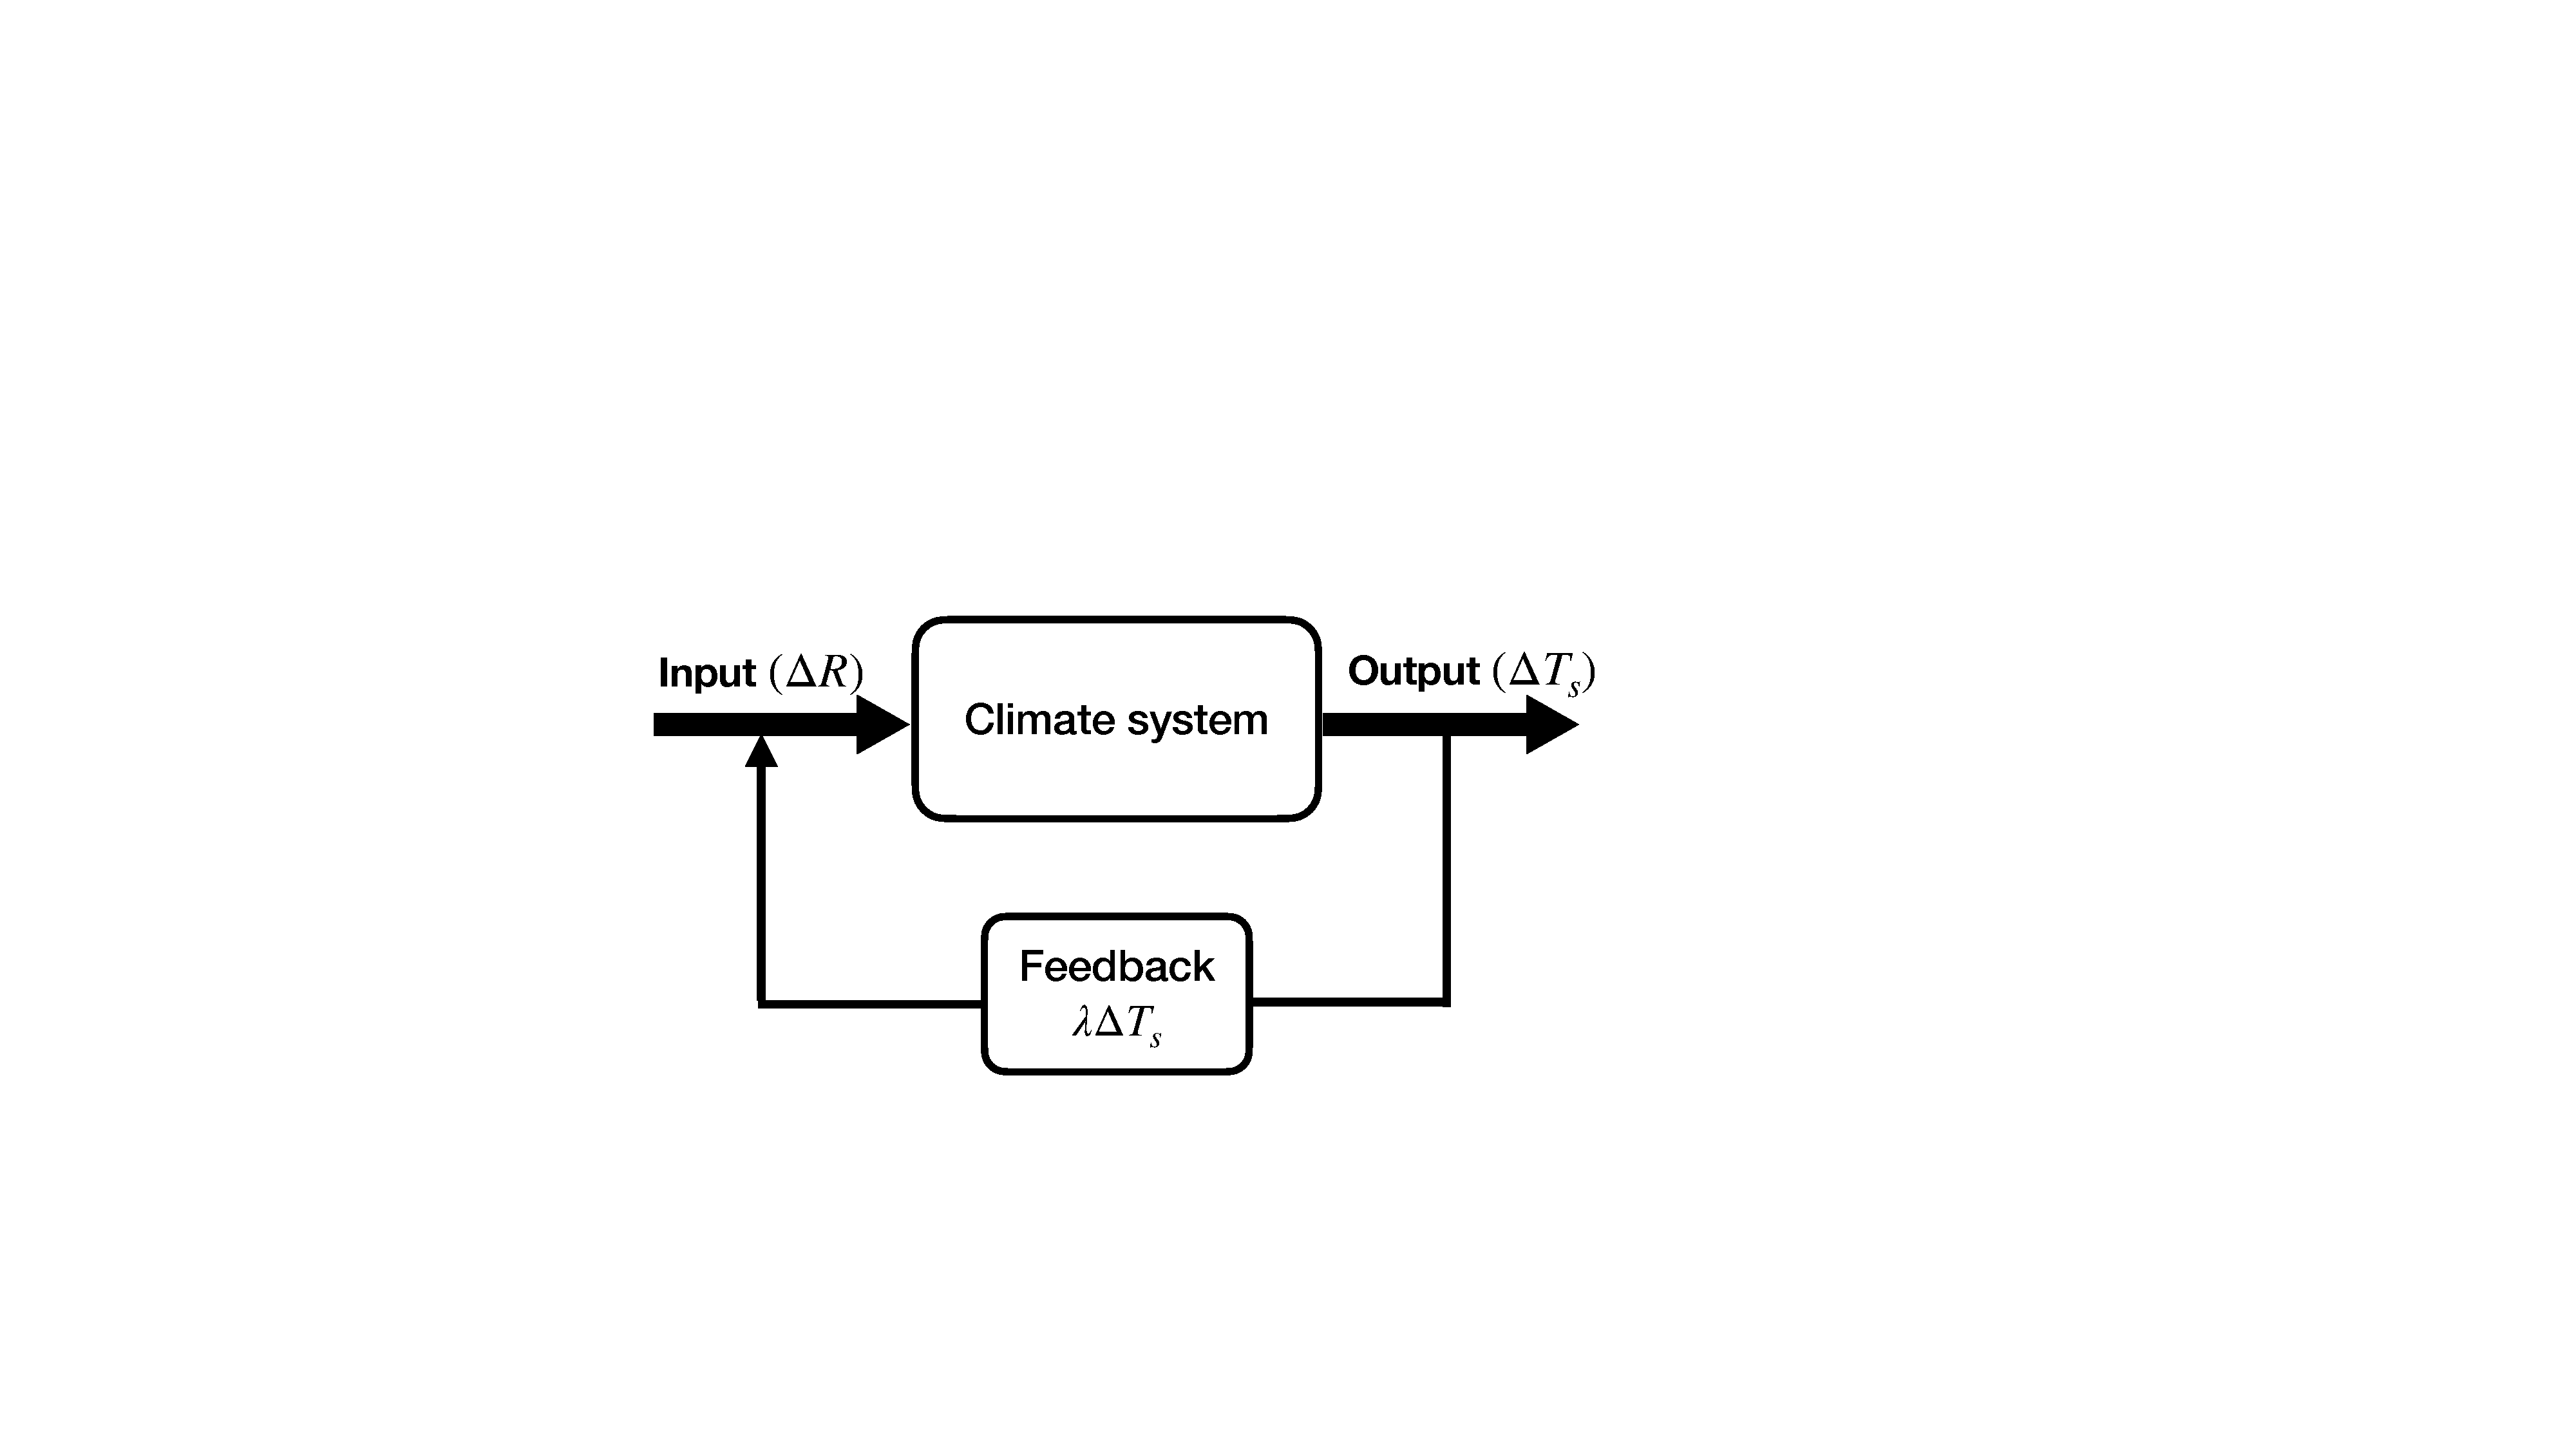
\includegraphics[width=0.6\linewidth]{{figs/literature_review/clim_system_feedback}.pdf}
	\caption{Schematic of feedback in climate system. $\Delta R$ is the input disturbance to the climate system, $\Delta T_s$ is the change of surface temperature and $\lambda$ denotes the climate feedback parameter.}
	\label{fig:schematic_climate_feedback}
\end{figure}

%What is feedback?
The idea of feedback\index{feedback} is taken from the control system, which is used to understand the system response to different forcings \citep{Stephens2005cloud}. As shown in \figref{fig:schematic_climate_feedback}, $\Delta R$ is the input to climate system, which can be seen as the radiative forcing produced by changing the content of CO$_2$ or aerosol, or by other factors such as volcanic eruption. Then many features in the climate system (such as surface temperature, specific humidity) would change in response to this forcing. In general, we select the surface temperature ($T_s$) as a key output variable. The change in surface temperature (i.e. $\Delta T_s$) can in turn impact the radiative balance at the top of the atmosphere (TOA)\index{TOA}. That is to say the output response is fed back to the system. The feedback parameter ($\lambda$, units Wm$^{-2}$K$^{-1}$) is a measure of the strength of the feedback. As introduced in \chapref{ch:polaramplification} there are many different feedbacks in the climate system, and here we focus on the ones related to clouds.

\begin{figure}[ht]
	\centering
	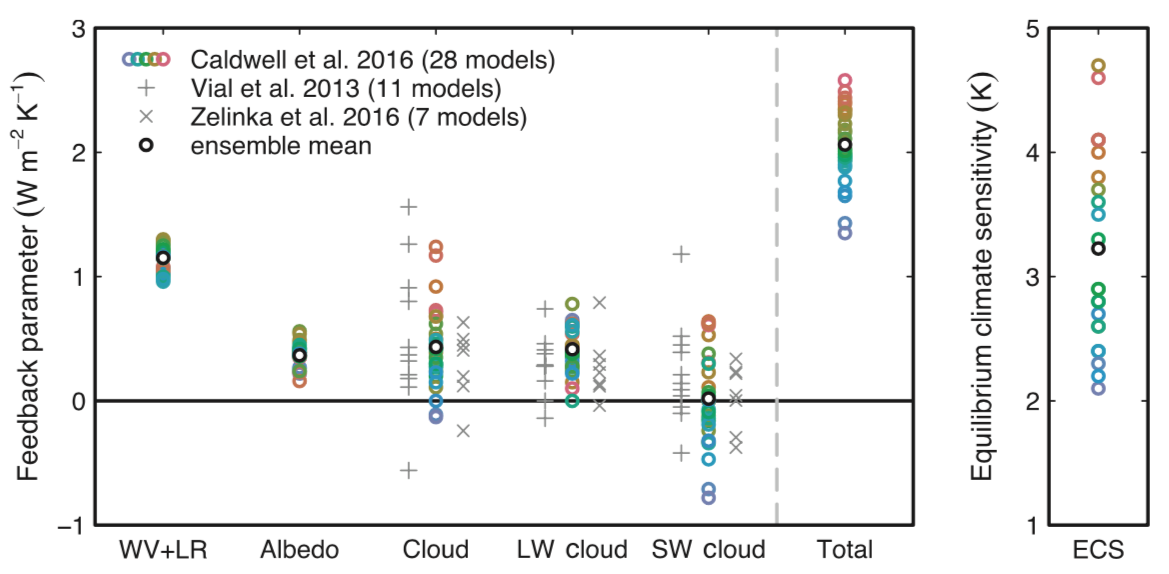
\includegraphics[width=1\linewidth]{{figs/literature_review/cloud_feedback_ceppi}.png}
	\caption{Strengths of individual global-mean feedbacks and equilibrium climate sensitivity (ECS) for CMIP5 models, derived from coupled experiments with abrupt quadrupling of CO$_2$ concentration. Circles are colored according to the total feedback parameter. The Planck feedback (mean value of -3.15 W m$^{-2}$ K$^{-1}$) is excluded from the total feedback parameter shown here. Adapted from \cite{Ceppi2017}.}
	\label{fig:cld_feed_back_ecs}
\end{figure}

Cloud feedback\index{cloud feedback} is the variation of cloud radiative forcing at the TOA in response to global warming. In the fifth assessment report of the Intergovernmental Panel on Climate Change (IPCC AR5), the sign of net cloud radiative feedback is likely positive with an estimate of 0.6 Wm$^{-2}$K$^{-1}$ \citep{stocker2013climate}, which, however, has a lot of uncertainties (-0.2 to 2 Wm$^{-2}$K$^{-1}$). As shown in Figure \ref{fig:cld_feed_back_ecs}, comparing to the water vapor, lapse rate and albedo feedbacks, cloud feedback is the largest uncertainty of simulated climate response to CO$_2$ foricng (i.e. climate sensitivity) in the general circulation models (GCMs) \citep{Ceppi2017}. Lots of efforts have been payed to investigate the possible reasons for the uncertainty of cloud feedbacks. For example, \cite{Webb2015} has proposed the Selected Process On/Off Klima Intercomparison Experiment (SPOOKIE) project, where the role of the convection has been accessed in the first phase of the project. They conclude that while parametrized convection influences the strength of the cloud feedbacks substantially in some models, other processes must also contribute substantially to the overall inter-model spread. In the second phase, the role of cloud scheme will be examined. For example, \cite{Geoffroy2017} found that the stratiform cloud scheme does play an important role in the spread of cloud feedback among the GCMs, both in stratocumulus regions and globally.

%, where the cloud fraction, cloud water content and effective cloud droplets radius are prescribed or will be diagnosed empirically.

A recent study by \cite{Sherwood2020} estimates that total cloud feedback is 0.45 Wm$^{-2}$K$^{-1}$ and the uncertainty (0.12 to 0.78 Wm$^{-2}$K$^{-1}$) is narrowed compared to the results from IPCC AR5. Nevertheless, the uncertainty of cloud feedback is still the largest one among all the feedback parameters (see Table 1 of \citealt{Sherwood2020}) and has no clear reduction from CMIP5 to CMIP6 (see Figure 4 of \citealt{Sherwood2020}).

%Cloud feedback decomposition? 
To fully understand cloud feedback is a challenging job, partly due to the diversity of clouds in climate system \citep{Zelinka2017}. For example, there are many different types of clouds, which are located at different locations and in different shapes or forms (such as liquid, ice or mixed phase), thus affecting the radiation in different ways. In addition, these clouds are usually controlled by different meteorological factors, therefore it is hard to predict the responses of clouds under climate change. Nevertheless, lots of efforts have been paid by previous studies to pin down the cloud feedback and here are some progresses. To make it clear, the cloud feedbacks are grouped into three categories: cloud amount, cloud altitude and cloud opacity feedbacks \citep{Zelinka2017}.

% cloud amount, cloud altitude, cloud opacity

\subsection{The features of cloud feedback}

\begin{figure}[ht]
	\centering
	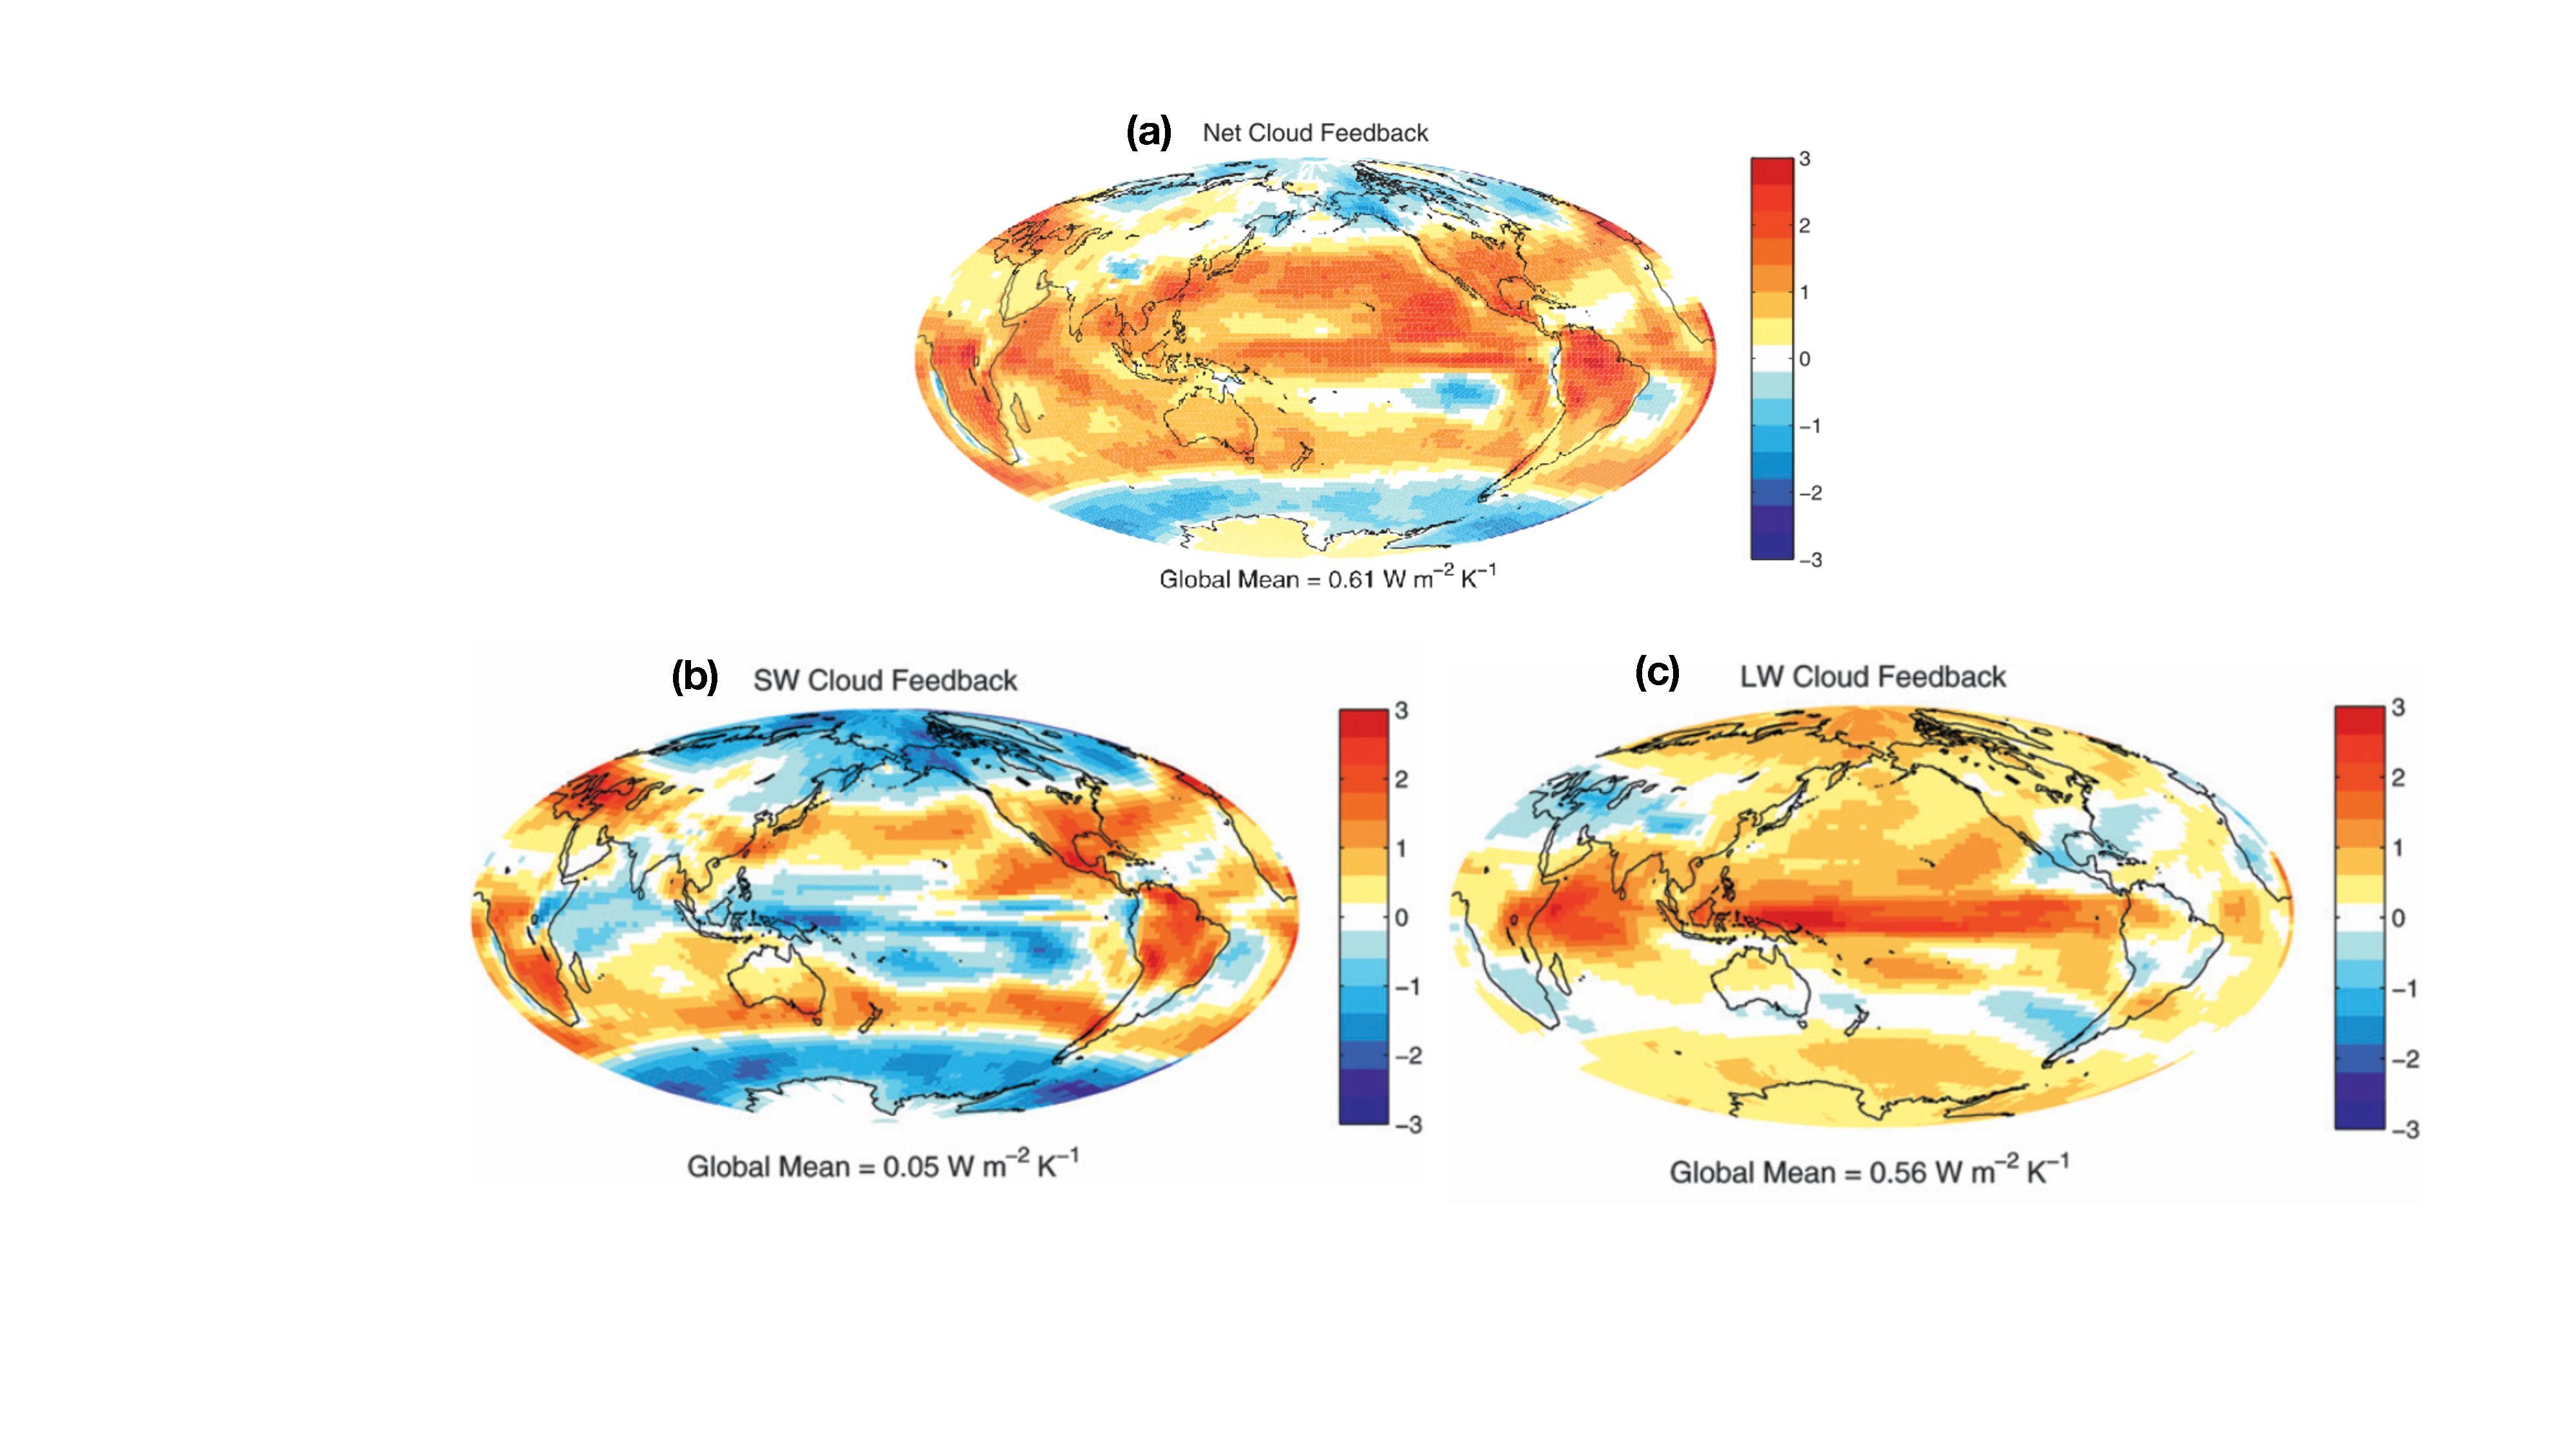
\includegraphics[width=1\linewidth]{{figs/literature_review/cloud_feedback_Zelinka_and_Hartmann2012}.pdf}
	\caption[The spatial patterns of net, SW and LW cloud feedbacks.]{Ensemble mean (a) net, (b) SW and (c) LW cloud feedbacks from 12 CMIP3 models, which are computed through the radiative kernel technique. Adapted from Figures 1 and 2 of \cite{Zelinka2012climate}.}
	\label{fig:spatial_pattern_of_cld_feedbacks_Zelinka}
\end{figure}

As shown in \figref{fig:spatial_pattern_of_cld_feedbacks_Zelinka}a, the net cloud feedback is positive at nearly every location equatorward of 45$^\circ$, and negative in most locations poleward of that latitude. When decomposing the net cloud feedback into LW and SW ones, we can find that the SW cloud feedback is negative in lower and high latitudes, but positive over the subtropics. For instance, the SW cloud feedback is negative in Southern Ocean region (\figref{fig:spatial_pattern_of_cld_feedbacks_Zelinka}b); while the LW cloud feedback is positive in almost everywhere and is pronounced at tropical regions (\figref{fig:spatial_pattern_of_cld_feedbacks_Zelinka}c). The possible mechanisms for these feedback patterns will be explained below.

\begin{figure}[ht]
	\centering
	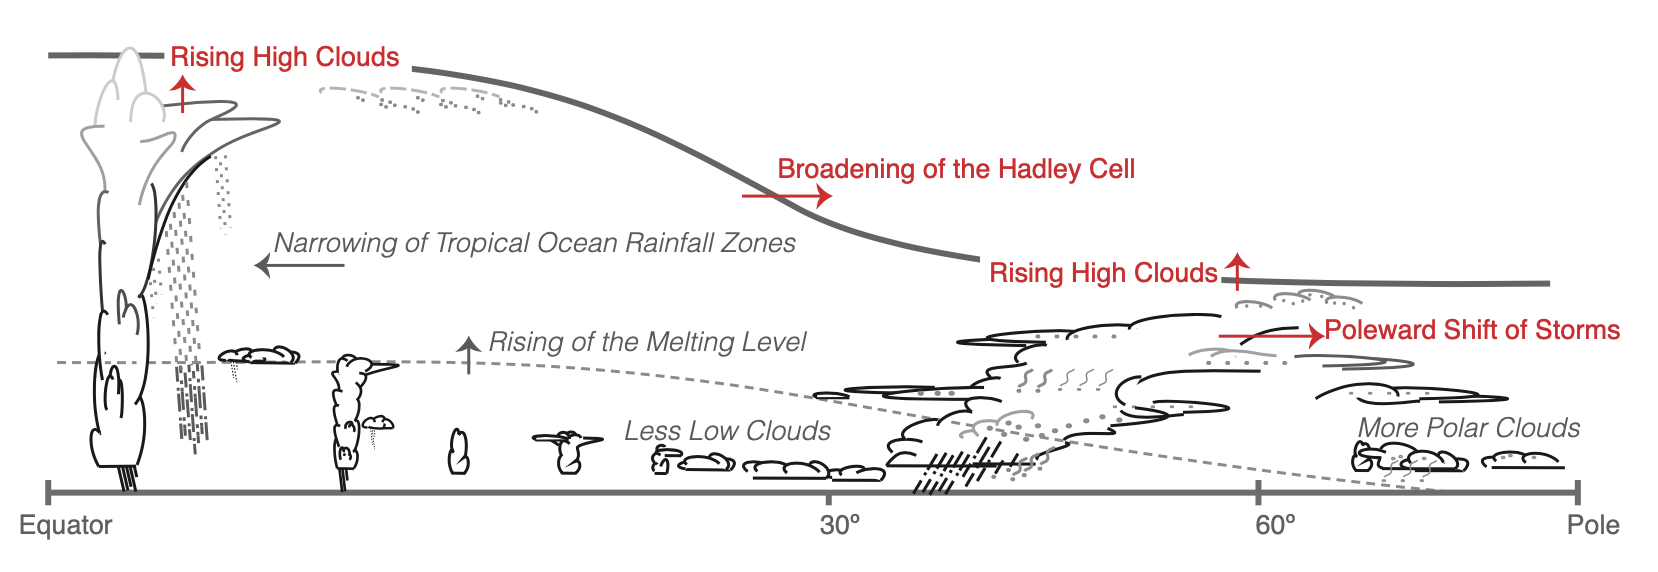
\includegraphics[width=1\linewidth]{{figs/literature_review/robust_cloud_responses_to_greenhouse_warming}.png}
	\caption[Robust cloud responses to greenhouse warming from IPCC AR5.]{Robust cloud responses to greenhouse warming. Adapted from Figure 7.11 of IPCC AR5 \citep{stocker2013climate}.}
	\label{fig:robust_cld_responses_ar5}
\end{figure}

Although the inter-model spread of cloud feedback is still large, and the sign of global mean cloud feedback is likely positive (e.g., 0.61 Wm$^{-2}$ in \figref{fig:spatial_pattern_of_cld_feedbacks_Zelinka}a). The major reasons are related to changes of three kinds of clouds as shown in \figref{fig:robust_cld_responses_ar5}: rising of high clouds, less subtropical clouds and more polar clouds as a result of reduced sea ice.

It is believed that the positive LW cloud feedback in tropical region is related to the rising of high clouds (\figref{fig:robust_cld_responses_ar5}) based on the fixed anvil temperature (FAT) hypothesis, which is first proposed by \cite{Hartmann2002FAT}, and used by lots of later studies \cite[e.g.,][]{Kuang2007,Zelinka2010longwave,Yoshimori2020fixed}. The FAT theory holds that the isotherms move up and convection deepens in tropical region as climate warms, but the cloud-top temperature of anvils remains approximately constant. In this case, the cloud-top temperature do not warm in step with the suface warming and the outgoing longwave radiation (OLR) keeps relatively constant, so the tropics become less efficient at radiating the heat away, indicating the high clouds act as a positive feedback on climate.

% The tro- popause and melting level are shown by the thick solid and thin grey dashed lines, respectively. Changes anticipated in a warmer climate are shown by arrows, with red colour indicating those making a robust positive feedback contribution and grey indicating those where the feedback contribution is small and/or highly uncertain. No robust mechanisms contribute negative feedback. Changes include rising high cloud tops and melting level, and increased polar cloud cover and/or optical thickness (high confidence); broadening of the Hadley Cell and/or poleward migration of storm tracks, and narrowing of rainfall zones such as the Intertropical Convergence Zone (medium confidence); and reduced low-cloud amount and/or optical thickness (low confidence). Confidence assessments are based on degree of GCM consensus, strength of independent lines of evidence from observations or process models and degree of basic understanding.

Compared to the LW cloud feedback of high anvil clouds, the SW cloud feedback still ``lacks a well-accepted theoretical basis" \citep{stocker2013climate}. From then on, many studies have tried to understand the causes of SW cloud feedback. 

Another stark feature in \figref{fig:spatial_pattern_of_cld_feedbacks_Zelinka}a is the negative cloud feedback in Southern Ocean area \citep[Figure 8 of ][]{Vial2013,Zelinka2012computing}. This is probably due to the phase change of clouds from ice to liquid, and the poleward shift of jet might be not important \citep{Kay2014processes}. This is a negative feedback because cloud liquid is more reflective than ice for a fixed cloud condensate amount, so less sunlight is absorbed by the atmosphere. Beyond this negative optical feedback or opacity feedback, another negative feedback also exists.

%Zelinka2020causes

\subsection{Cloud amount feedback}
% the cloud top of these clouds are usually high, meaning a low temperature at cloud top. 
The feedback induced by the cloud amount change is different for different cloud types. Specifically, the warming-induced increase of high, thin clouds usually leads to a positive feedback. The reason is that the optical depth of these high, thin clouds is typically small, thus having little impact on the shortwave radiation. However, the clouds can absorb the longwave radiation and thus constitute a strong greenhouse effect (XXXXXXX some reference). In contrast, the warming-induced increase in the amount of low clouds (opaque ones) brings a negative feedback as less sunlight can reach the surface, thus a cooling effects. These are the two typical cloud amount feedbacks.

Low clouds

marine low cloud changes are well described by reductions in low cloud fraction in response to local SST increases \citep[e.g.,][]{Rieck2012, Webb2013coupling, Qu2014, Bretherton2015, Brient2016,Ceppi2017relationship} and increases in low cloud fraction in response to increases in lower-tropospheric stability...This suggests that low cloud changes depend on local SST changes and remote effects that influence free tropospheric temperatures and hence lower-tropospheric stability \citep[e.g.,][]{Zhou2015,Zhou2016,Zhou2017,Andrews2018}. 

The formation and dissipation of low clouds are controlled by the differences between the supply of moisture from the surface and the mixing of relatively dry air above the boundary layer. The processes can be influenced by many large-scale meteorological factors, including sea surface temperature (SST), estimated inversion strength \citep[EIS;][]{Wood2006}, the relative humidity in the free troposphere, the strength of large-scale subsidence, warm/cold temperature advection and surface wind speed \citep{Scott2020}. The detailed effects are as follows:

\begin{enumerate}[label={(\arabic*)}]
    \item SST \\
    Warmer SST leads to the higher temperature and saturation water vapor pressure in the boundary layer, and can weaken the inversion strength if the temperature in the free troposphere remains constant. In this case, the in-cloud latent heating 
    \textcolor{red}{(I don't know why SST can influence the in-cloud latent heating?)} enhances the turbulance and entrainment of the drier air from aloft into the boundary layer, thus resulting in the reduction of cloudiness in low level.
    
    \item EIS \\
    Stronger EIS means more energy needed to mixing the relatively dry free-tropospheric air into the boundary layer and more moisture is trapped below the inversion layer, thereby favoring more low-level clouds.
    
    \item Subsidence \\
    Stronger subsidence can push down the boundary layer much lower and make the clouds lower and thinner, thereby supporting less low-level clouds.
    
    \item Moisture in free troposphere \\
    If the relative humidity in free troposphere is large, then the cloud-top entrainment drying is weaker, which thus favors more low-level clouds.
    
    
    At the same time, more free-tropospheric moisture emits more downwelling LW radiation, which can weaken cloud-top radiative-cooling and the overturning circulations that mix moisture up from the surface, thereby favoring less low-level cloud
    
    
    \item Warm/cold temperature advection\\
    %Stronger warm (cold) temperature advection in the boundary can lead to stronger upward (downward) latent heat flux
    Low-level advection from cold to warm SST brings relatively cool and dry air over warmer water, which triggers enhanced upward turbulent fluxes of heat and moisture from the sea surface, providing a strong source of moisture for cloud formation.
    
    Conversely, low-level airflow from warm to cold SST brings relatively warm and moist air over cooler water, which stabilizes the boundary layer and cuts off clouds from the surface moisture supply. 
    
    \item Surface winds\\
    Stronger winds increase evaporation from the sea surface and promote deepening of the boundary layer.
    
\end{enumerate}


\subsection{Cloud altitude feedback}

\subsection{Cloud opacity feedback}


\subsection{Role of cloud schemes in cloud feedback}

%Roles of parameterizations to the spread of cloud feedback among GCMs

Previous studies have shown that many parameterization schemes such as boundary layer and shallow convection can have impact on the spread of cloud feedbacks in GCMs \cite[e.g.,][]{Gettelman2012,Zhang2013CGILS,Sherwood2014spread}.
However, this inter-model spread did not decrease after the convective parametrizations being turn off \citep{Webb2015}, indicating that the difference in convection pramameterization schemes is not the main cause for inter-model spread of cloud feedback and other processes must also contribute substantially to the overall inter-model spread.

\cite{Zhang2013CGILS} proposed a mechanism to explain the positive subtropical low cloud feedback in climate models, in which the increased entrainment of dry air from the free troposphere into the boundary layer by parametrized convection in the warmer climate reduces low cloud amounts.

%For example, \cite{Sherwood2014spread} pointed out that the strength of convective mixing between the lower and middle tropical troposphere can explain about half of the variance in climate sensitivity estimated by GCMs. \cite{Zhang2013CGILS} showed that the differences in shallow convection schemes are causes of different cloud feedbacks in the models.

% The net cloud feedbacks can be considered as due to two opposing roles of surface-based PBL turbulence and shallow convection aided by cloud-top entrainment. \cite{Zhang2013CGILS} 

\cite{Geoffroy2017} implemented a range of diagnostic cloud schemes into two climate models (CAM4 and CSIRO-Mk3L) in lower troposphere, and found that roughly half of the multi-model spread in the cloud feedback in stratocumulus regions could be reproduced by changing the stratiform cloud scheme alone. In addition, they found that total water probability density function (PDF)-based schemes (see more in \secref{sec:PDF_cld_scheme}) tend to impose a positive low cloud feedback, while the stability dependent schemes tend to produce a negative feedback. These are similar to the findings of \cite{Qu2014}, in which they find the PDF-based schemes predict low cloud cover reduction in the stratocumulus regions, whereas most models employing schemes with stability dependent cloud fraction predict opposing changes in the same regions. In this case, it seems that stability dependence plays an important role in determining the sign of cloud feedback, which, however, does not fully determine the sign of cloud feedback, including in marine stratus regions \citep{Geoffroy2017}.

%\cite{Sherwood2010}

%\section{Cloud Radiative Effect and its feedback}

\section{Cloud-circulation coupling}
\label{sec:cld_circulation_coupling}

As introduced in previous section, in climate system clouds modulate the flow of energy by interacting with radiation, which then can have an impact on the circulation.

\cite{Voigt2020review}

\section{Cloud schemes}
\label{sec:cld_scheme_history}
\index{cloud scheme}
\subsection{Overview}

\begin{figure}[ht]
	\centering
	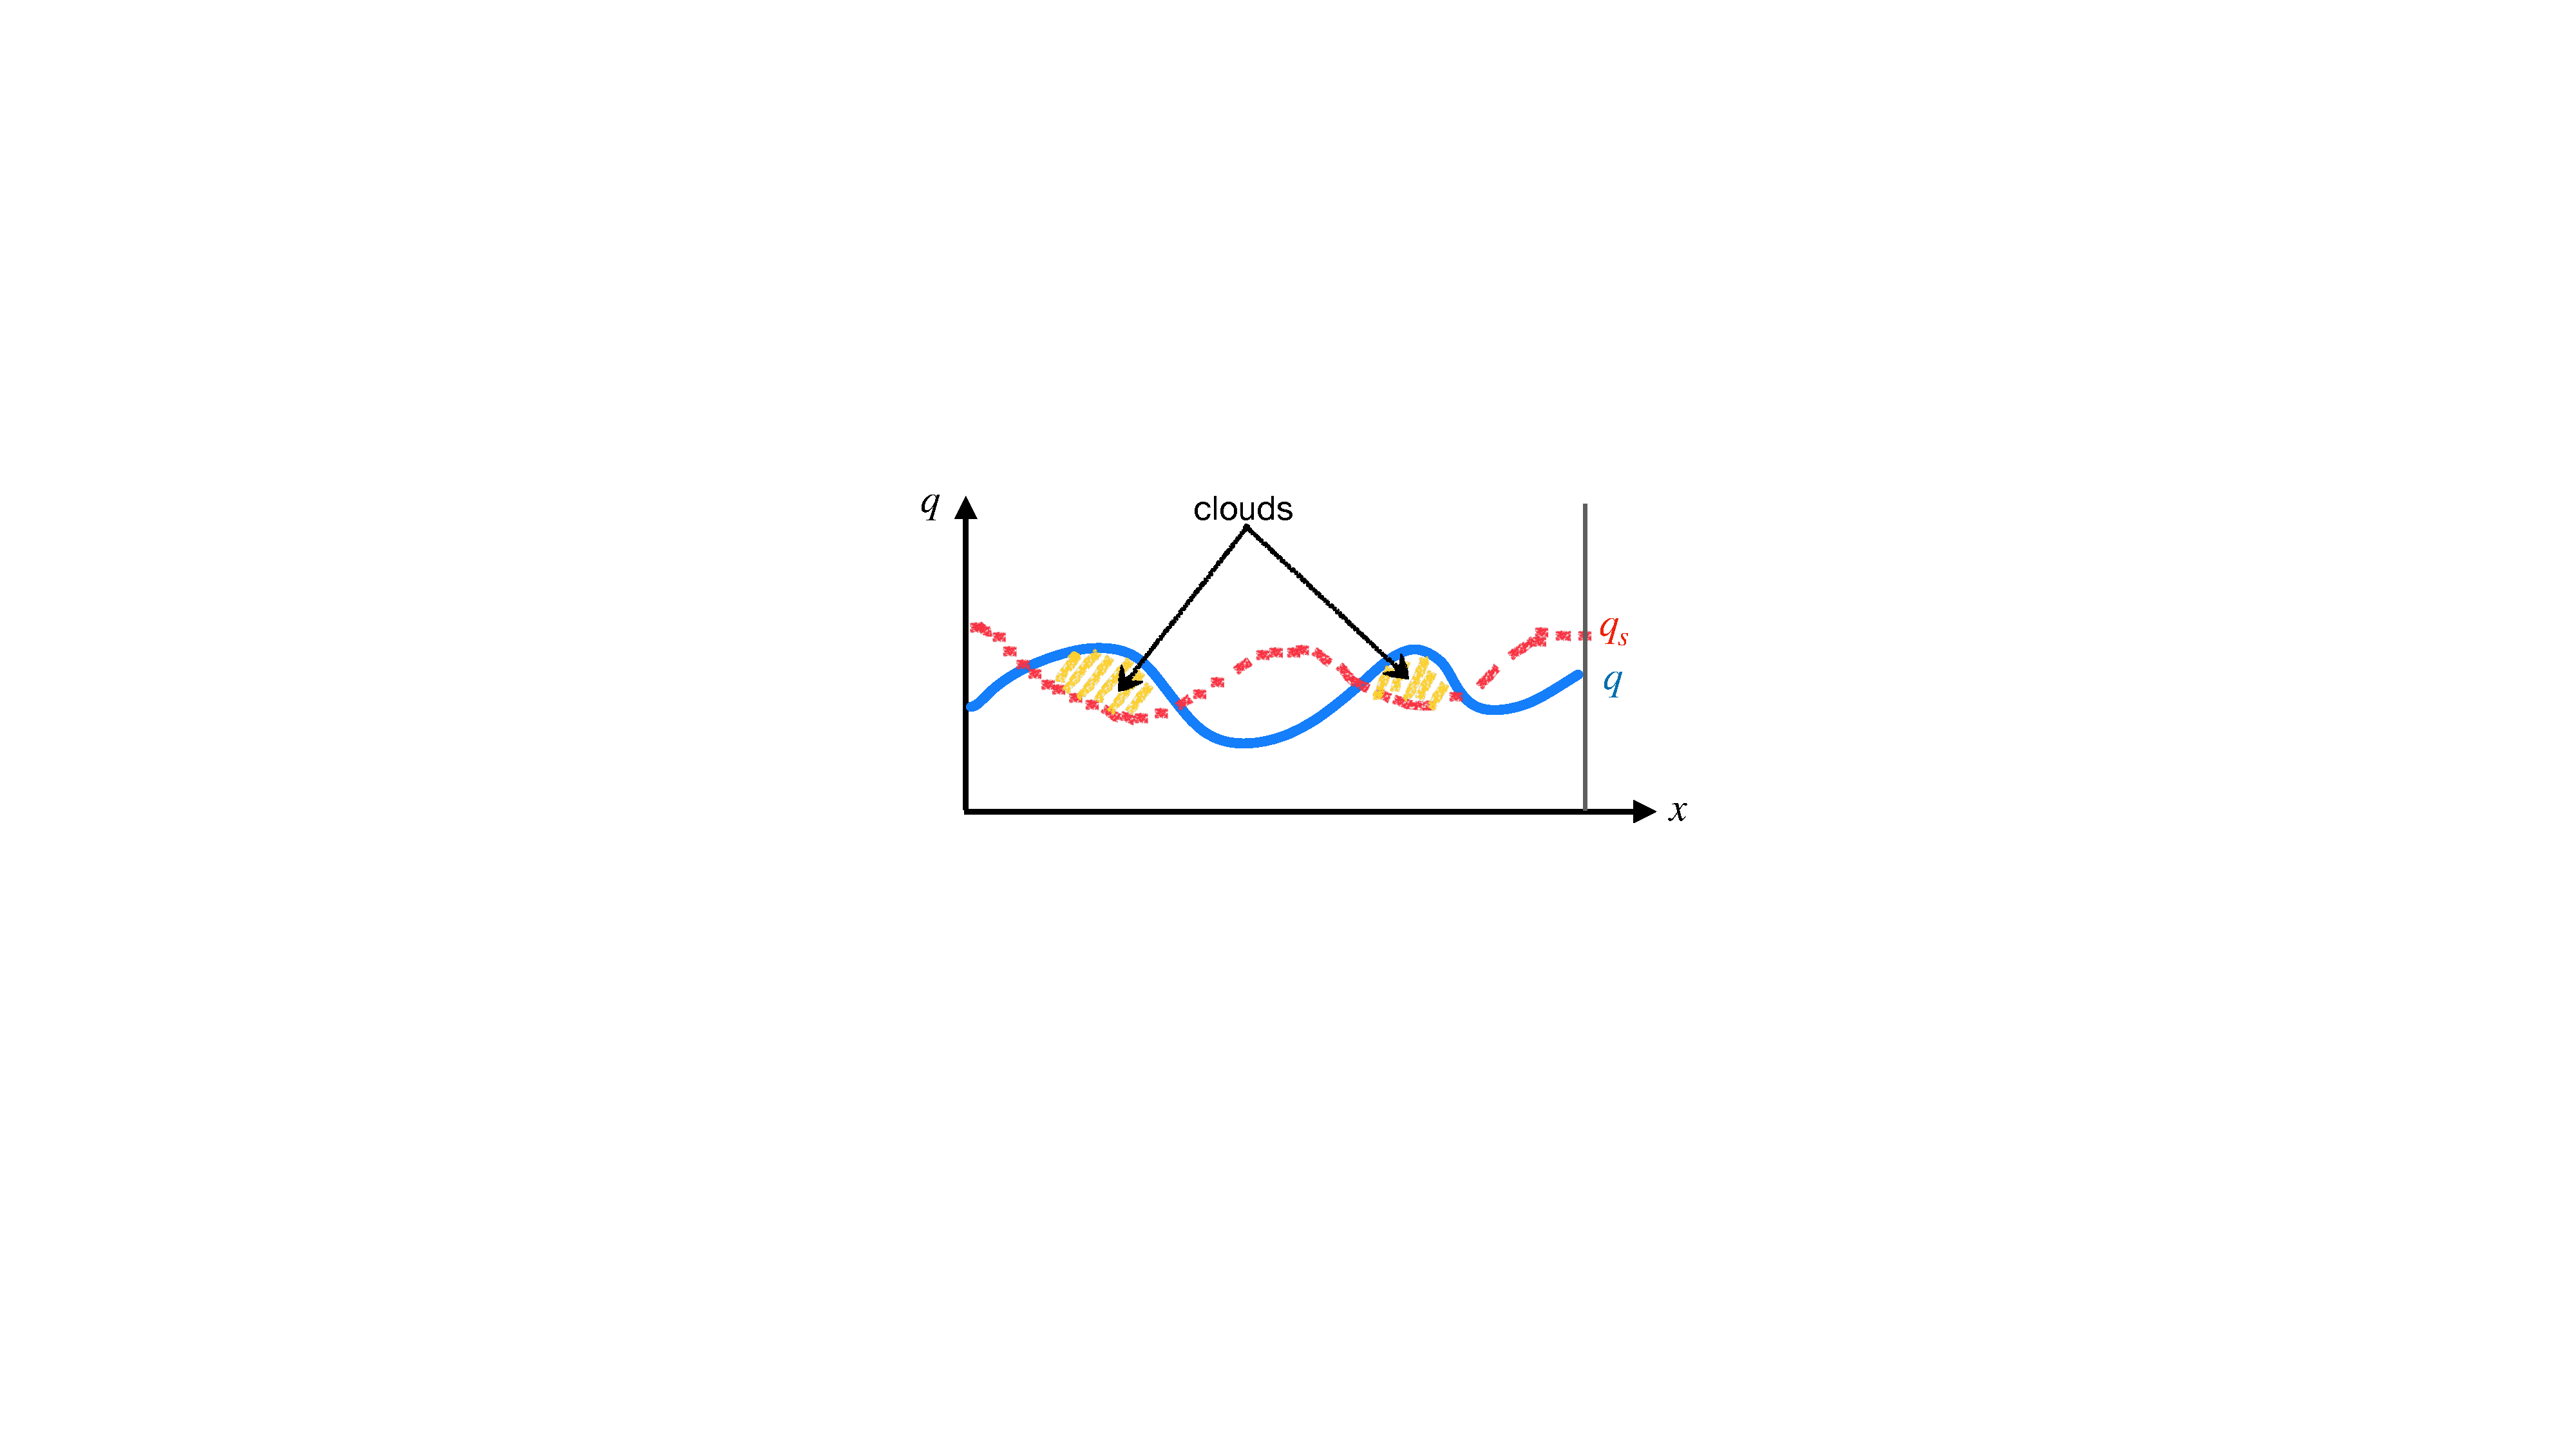
\includegraphics[width=0.8\linewidth]{{figs/literature_review/Schematic_partial_cloud_cover_in_gridbox}.pdf}
	\caption{Schematic showing that partial cloud cover in a grid box (1D) when temperature or humidity fluctuations exist. The blue line shows humidity and the red dashed line indicates saturation mixing ratio of the grid box. The shaded regions are cloudy parts as the humidity exceeds the saturation mixing ratio.}
	\label{fig:schematic_partial_clouds}
\end{figure}

At present the typical horizontal resolution of the GCMs is 50-200km, but the clouds usually involve the air motions in mesoscale and convective scale \citep{Houze2014}, which are usually in sub-grid scale both horizontally and vertically, implying that cloud processes are hard to be explicitly resolved by the GCMs. In this case, the ``parameterization" becomes a practical way to build cloud schemes. The parameterization is to represent the effects of the smaller-scale processes (turbulence, cloud microphysics, convection, etc.) in terms of the large-scale states (such as velocity, temperature, pressure, humidity) \citep{Randall2003}, which could be seen as a way to find potential relationships between the unknown and known variables \citep{Randall1989}.


\subsection{Relative humidity schemes}
\index{cloud scheme!RH scheme}
Previous studies have investigated various ways to represent clouds in climate models. For example, \cite{Holloway1971} prescribed the clouds externally with climatological data without dynamic interplay with the other components of the model. Some early modelling studies made the assumption that a grid box in the model is either fully saturated or totally unsaturated. However, this assumption is not reasonable enough as the humidity can distribute unevenly within a grid box, suggesting that condensation can occur even the relative humidity is less than 100\%. A general idea is to link the cloud cover with the relative humidity, as one can expect that the amount of condensation would increase with the increase of mean humidity of the model grid box, which is the basis for some diagnostic methods.

Diagnostic schemes predict the cloudiness based on the model variables empirically or statistically. In these schemes, the clouds can be linked to atmospheric outputs such as relative humidity, vertical velocity and static stability, among which the linear relationship between cloud fraction against RH could be simplest one. For example, \cite{Smagorinsky1960} found empirically that non-convective cloud amount correlated with the average relative humidity in the respective layers (\figref{fig:Smagorinsky_RH_cld}), arguing that the non-precipitating condensation depend only on the accumulated history of vertical motion, which can be reflected by the humidity. \cite{Ricketts1973} obtained roughly linear relationship between cloud amount and observed relative humidity but commented that the relationship is somewhat indefinite.

Water vapor generally distributes heterogeneously in the grid box, so the averaged RH within a box should be less than 1 for a partial coverage of clouds. Previous studies usually adopt the critical relative humidity $RH_{crit}$ as the minimum threshold for clouds to form, which is often left as a free parameter that can be tuned during model development (e.g. \citealp{Hourdin2017,Kay2012,Mauritsen2012}). For example, \cite{Sundqvist1978} and \cite{Sundqvist1989} find that cloud fraction can be rewritten as a function of critical RH by assuming the water vapour is uniform distributed within the grid box. In general, $RH_{crit}$ decreases with height, but will vary according to different types of clouds. Although the $RH_{crit}$ doesn't have clear physical meaning, it can be used to modify the cloud amounts in different locations. For example, one can increase $RH_{crit}$ asymptotically to nearly unity to prevent the unrealistic circus clouds \citep{Sundqvist1989}. 

As a unique predictor, RH is very simple and useful to diagnose the cloudiness, and it is still widely used in GCMs \citep[e.g.,][]{Gordon1992,Park2014,Pope2000}. However, it is not valid for all the cases. As we can see, some studies also made use of other variables to diagnose the cloudiness. For instances, \cite{Xu1996} developed a semi-empirical scheme to determine the stratiform cloud fraction based on grid-averaged mixing ratio of condensate (cloud water and cloud ice) and RH. As for the scheme provided by \cite{Slingo1987}, both the RH and vertical velocity were taken into account, in which different empirical relations were used for different clouds including low, middle, high and convective clouds.

In summary, the methods based on relative humidity and other predictors are useful to diagnose the cloudiness, which ensures that the clouds can form before the grid box get saturated. One problem for the diagnostic methods is that in most cases the cloud condensate has to be diagnosed or prognosed via other methods \citep[e.g.,][]{Zhang2003, Park2014}, which could lead to some inconsistencies between cloud fraction and cloud condensate (e.g. \citealp{Gregory2002, Tompkins2005}).

\begin{figure}
	\vspace{-0.3cm}
	\centering
	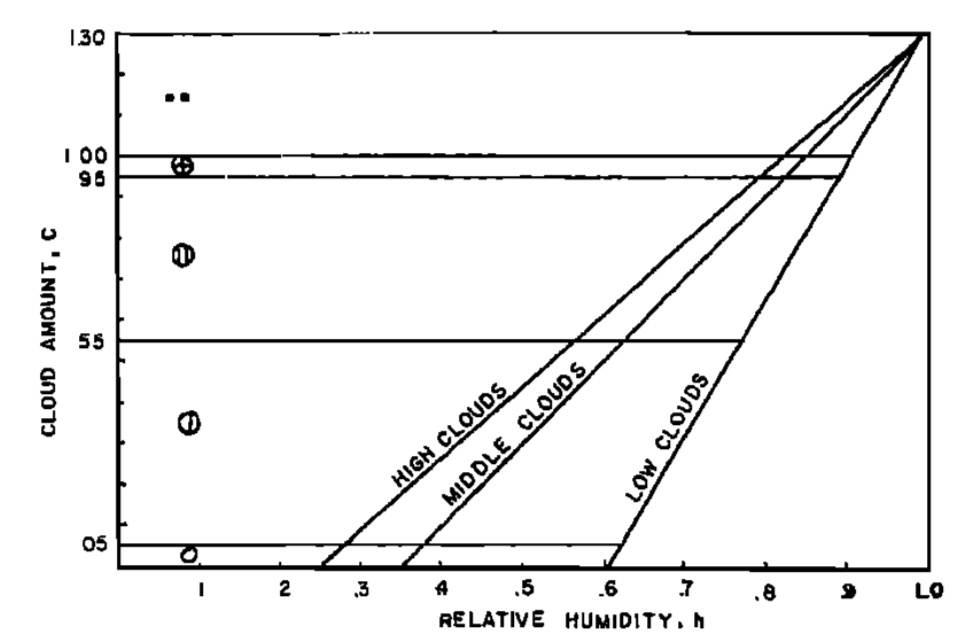
\includegraphics[width=0.6\linewidth]{{figs/literature_review/Smagorinsky1960}.png}
	\caption{Empirically determined relation of mean relative humidity $h$ in the layers 1000-800mb, 800-550mb and 550-300mb with cloud amount $c$ classed as low, middle and high clouds. Adapted from Figure 1 of \cite{Smagorinsky1960}.}
	\label{fig:Smagorinsky_RH_cld}
\end{figure}


\subsection{Statistical schemes}
\label{sec:PDF_cld_scheme}
\index{cloud scheme!statistical or PDF scheme}

In contrast, the prognostic approach \citep[e.g.,][]{Tiedtke1993} is to explicitly calculate the clouds related variables, such as cloud water content, in order to pursuing a unification of all clouds processes, which is more realistic in some degree and requires more physical basis and interactions with other parts of the models. Another widely used cloud prediction method is statistical scheme, in which the cloud fraction and in-cloud liquid water/ice are determined based on the assumed probability distributions of subgrid variability of thermodynamic properties. As the cloud related variables such as moisture and temperature are not the same everywhere but distributed randomly within the grid box, it is natural to assume that the cloud cover depends on the distribution of moisture, sometimes on the joint distribution of moisture and temperature. As shown in a very early work, \cite{Sommeria1977} gave up the assumption that a grid is either entirely saturated or unsaturated in the climate models and proposed the idea to use the statistical distribution of moisture within the grid box. For example, given the probability distribution function (PDF) of the total water ($q_t$ is the mixing ratio) in grid box, the cloud fraction ($CF$) can be calculated as 
\begin{equation}
    CF=\int_{q_s}^{\infty}\text{PDF}(q_t)\operatorname{d}q_t,
\end{equation}
and the cloud water content ($q_c$ is the mixing ratio of cloud water) is
\begin{equation}
    q_c=\int_{q_s}^{\infty}(q_t-q_s)\text{PDF}(q_t)\operatorname{d}q_t,
\end{equation}
where $q_s$ is the saturation mixing ratio in both formulations.

However, the shapes of subgrid-scale PDF of total water specific
humidity, saturation deficit, or a combined variable of liquid water and potential temperature are difficult to determine due to limit of observational data, so sometimes the model data are also used \citep{Bony2001}. Additionally, many different forms PDF have been proposed in the previous studies. For example, \cite{LeTreut1991} made use of the uniform distribution of total water in the grid box to calculate the clouds cover and liquid water content. Other symmetrical distributions, such as Gaussian distribution \citep{Sommeria1977}, triangular distribution \citep{Smith1990} and skewed distributions, such as lognormal distribution \citep{Bony2001} and beta distribution \citep{Tompkins2002}, have also been employed in numerical models. However, there are also some problems in the distributions. For example, the Gaussian distribution is unbounded, indicating that the maximum cloud condensate mixing ratio might approach infinity, and cloud cover is always large than zero \citep{Tompkins2002}. In general, complicated forms of the PDF need more parameters to fit. But due to the limitation of the data, it is possibly hard to validate the distributions. Linking the statistical cloud scheme to other physical processes seems a promising way to improve cloud simulations. For example, \cite{Qin2018} developed a Gaussian PDF cloud scheme with the PDF variance diagnosed from the turbulent
and shallow convective processes, which could improve the simulation of low marine clouds and alleviate double Intertropical Convergence Zone (ITCZ) problem \citep{Qin2018alleviated}.

The statistical cloud schemes may have better performance than the diagnostic ones, but considering the fact that there is no clouds scheme in Isca currently, it would be useful to implement the simple diagnostic schemes in Isca first, which can be seen as the first step to implemented a hierarchy of cloud schemes.

\subsection{Relationship between relative humidity and statistical schemes}

As discussed in previous section, one has to determine the expression of sub-grid variance (i.e. second order moment) or other higher-order moments in the statistical schemes. In doing so there are two general practices in current studies. The simple case is to use the time-invariant variance \citep[e.g.,][]{Sundqvist1978,Smith1990}, and the other approach is to employ time varying variance, which are usually obtained from other physical processes such as boundary layer scheme or shallow convection schemes \citep[e.g.,][]{Qin2018}. The second case usually provides a more realistic link between clouds and other physical processes \citep{Tompkins2002}. 

Note that there is no distinction between the RH schemes and statistical schemes, although they seem different in forms. As a matter of fact, if the subgrid variance in a statistical scheme is assumed to be time-invariant, it can be reduced to a RH scheme \citep{Tompkins2002,Tompkins2005}. The key is to link the variance with the critical relative humidity. That is to say, critical RH value can reflect the level of sub-grid variance in RH schemes \citep{Quaas2012}. Larger critical RH value means the lower subgrid variability and vice versa. For example, the \cite{Sundqvist1978} RH scheme can be derived by assuming a uniform distribution of total water mixing ratio within a grid box, in which the variance is assumed a constant fraction of the saturation water vapor mixing ratio, and this constant is associated with critical RH value (see Appendix A of \cite{Quaas2012} for a full derivation). Another example is the triangular distribution used by \cite{Smith1990} and \cite{Park2014}, they also obtain the equivalent RH formulation by assuming the variance is related to critical RH. As pointed by \cite{Tompkins2002}, the parameterizations such as \cite{Xu1996}, in which cloud fraction is related to RH and cloud condensate, can be viewed as manifestations of a statistical scheme although where the actual PDF of total water is not known. %, but the time-mean statistics of its integral are.

\section{Aims of the study}
\label{sec:why_simple_cld_schem_in_isca}
% This section introduce our goal to do for this phd study

The question then arises as to what a `simple' scheme is. One option would be to specify the PDF of total water within a grid box. Then, supposing that cloud formation occurs on saturation, one may be able derive a functional relation between mean cloud amount and mean relative humidity, supposing that the latter is what is predicted by the GCM from its predictions of specific humidity and temperature. \citet{Sundqvist1989} scheme was motivated this way, where the uniform distribution is adopted and variance of the distribution is assumed to be time-invariant \citep{Tompkins2005}. Although such a procedure is physically motivated it has two potential drawbacks. First, deciding on a distribution of humidity is somewhat arbitrary, or involves turbulence closure assumptions used in the stochastic model \citep{Sommeria1977,Tsang2018}. Second, translating the prediction of a probability distribution into a practical cloud model may be problematic, for there is in general no straightforward translation from a humidity probability distribution to an analytic formula connecting fractional cloud cover to relative humidity. 

Thus, here we chose another course by linking the cloud cover with the relative humidity ab initio. We explore two schemes, one with a piecewise linear relationship between cloud cover and relative humidity and the other with a square-root relationship, as in \citet{Sundqvist1989}. The various coefficients entering into these schemes are obtained empirically, comparing results with observations. We also use the scheme in an idealized GCM, Isca \citep{Vallis2018}, configured with a realistic distribution of continents to explore the geographical variability of the cloud schemes. Idealized models have a number of advantages in investigating physical processes, especially when set within a hierarchy connecting them to more comprehensive models \citep[e.g.,][]{Maher2018_hierarchies, Thomson2019}. We find that a relative-humidity scheme alone is unable to capture the subtropical low cloud distribution but that this can be readily improved by the addition of a scheme that takes into account inversion strength. Similarly, we find that in high-latitudes the cloud radiative effect is improved by the addition of a `freeze-dry' scheme. 

In its most complete form the scheme is able to capture the main features of clouds on Earth to a level of accuracy (in both geographical and seasonal variability) similar to that of other contemporary, and much more complicated, schemes in comprehensive climate models. It does so in a very transparent fashion and the dependence on parameters can be made explicit. And although we have implemented the scheme in a particular GCM it could easily be ported to others, either by an ab initio but straightforward implementation or by porting the code itself. 

% Idealised climate models can be used, amongst other things, to investigate how clouds impact the large-scale circulation, see  for a review. For example, using the cloud locking approach or investigating the behaviour of a process in the absence of clouds, such as the Isca model that does not have clouds or water vapour feedbacks. For our purpose, the scheme should be simple enough to facilitate understanding of the role of clouds in the dynamics of climate variability and climate change, but complex enough to be able to capture the main features of clouds on Earth, comparable to that of other contemporary (and more complicated) climate models.

% We organize the paper as follows. Section 2 provides a description of the simple cloud scheme, SimCloud, including the methods to parameterize the cloud fraction and specify other needed physical parameters, such as the effective radius of cloud droplets and in-cloud condensate content. (Some of the choices and parameters used come from the experiments and observations described in later sections, but for clarity the cloud scheme is described first.) Section 3 describes the model and experimental configurations as well as the data sets used in this study. In Sect. 4 we compare the simulated cloud properties with observations, with an emphasis on the CRE. A discussion and conclusions are presented in Sect. 5.
% \chapter{Data and Methods}
\label{ch:methods}

In this thesis, several different observational and reanalysis data sets, as well as model simulations, are used. For example, the reanalysis data sets are employed in \chapref{ch:simple_cld_scheme} to derive the linear formula between cloud fraction and relative humidity, and to evaluate the relationship between low cloud amount and its possible proxies. The satellite products about clouds and radiation fields are used in \chapref{ch:eval_cld_scheme} to evaluate the performance of the simple cloud scheme. To make it clear, these data sets are briefly summarized in this chapter.

The major topic of this thesis is about the cloud feedback, and the main tool used to simulate it is the idealized climate model, Isca \citep{Vallis2018}. Therefore, the features of this climate model and the advantages of using the idealized models are discussed here. However, how to calculate or estimate cloud feedback in climate models is not so evident, and the direct estimate from the change of cloud radiative effect might be impacted by the cloud masking effect. Therefore, it is necessary to discuss the pros and cons of the several different methods to estimate cloud feedback in this chapter. Also, based on these discussion, it would be much easier for Isca to calculate the cloud feedback and decompose it into different components if the cloud simulator is implemented there, so the topic about this is also presented in this chapter. 

The chapter is organized as follows: The satellite data sets related to radiation and cloud fields are introduced in \secref{sec:obs_reanalysis_dataset}. The idealized general circulation model employed throughout this thesis is briefly described in \secref{sec:isca_intro}. In \secref{sec:cosp}, how the cloud observation simulator package is implemented in Isca is documented. \secref{sec:method_cloud_fbk} summarizes the possible methods to calculate the cloud feedback.

\section{Observational and reanalysis datasets}
\label{sec:obs_reanalysis_dataset}

%\subsection{Satellite datasets}
\subsection{Clouds and radiation data sets}
Satellites play important roles in observing the Earth over the past decades, and these satellite retrievals are essential data sets for us to understand the weather and climate on Earth. The observation of clouds and radiation at the TOA is particularly depend on the satellites. In general, the satellite products can be categorized into different groups according to their processing levels ranging from Level 0 to Level 4 \citep{Parkinson2006earth}. Specifically, Level 0 is the raw and unprocessed instrument data. Level 1 is annotated with ancillary information (1A) and processed to sensor units (1B). Level 2 is derived geophysical variables, Level 3 is mapped to a space-time grid, and Level 4 are modeled outputs or variables derived from multiple measurements. It is usually easier for users to use these satellite retrievals when they have higher processing levels.

% (see \url{https://earthdata.nasa.gov/collaborate/open-data-services-and-software/data-information-policy/data-levels}, last accessed: April 28, 2021)
% https://nsidc.org/the-drift/2013/08/is-it-1b-2-or-3-definitions-of-data-processing-levels/

% \begin{itemize}
%     \item \textbf{Level 0}:	Reconstructed, unprocessed instrument and payload data at full resolution, with the communications artifacts removed.
%     \item \textbf{Level 1A}: The Level 0 data with time-reference and with ancillary information
%     \item \textbf{Level 1B}: Same as Level 1A data, but have been processed to sensor units (not all instruments have Level 1B source data)
%     \item \textbf{Level 2}:	Derived geophysical variables at the same resolution and location as Level 1 source data.
%     \item \textbf{Level 3}:	Variables mapped on uniform space-time grid scales, usually with some completeness and consistency.
%     \item \textbf{Level 4}:	Model output or variables derived from multiple measurements.
% \end{itemize}


\subsubsection{Clouds and the Earth’s Radiant Energy System  Top-of-Atmosphere (TOA) data product}
% Energy Balanced and Filled (EBAF)

The Clouds and the Earth’s Radiant Energy System (CERES) project (\url{https://ceres.larc.nasa.gov}) provides satellite-based observations of Earth's radiation budget and clouds \citep{Wielicki1996clouds}. It uses measurements from CERES instruments flying on several satellites (TRMM\footnote{TRMM: Tropical Rainfall Measuring Mission, a research satellite in operation from 1997 to 2015}, Terra, Aqua, S-NPP\footnote{S-NPP: Suomi National Polar-orbiting Partnership}, NOAA-20\footnote{NOAA-20: National Oceanic and Atmospheric Administration-20}), along with measurements from higher-resolution imagers on polar orbiting and geostationary satellites and other input data source, to produce a comprehensive set of Earth's radiaiton budget data products for weather, climate and applied science research. The goal of CERES is to produce a long-term, integrated global climate data record for detecting the possible changes in the Earth’s radiation budget from the surface to the top of the atmosphere, so as to improve our understanding of how Earth’s radiation budget varies in time and space and of the role that clouds and other atmospheric properties play.

The main CERES product used in this thesis is the Energy Balanced and Filled (EBAF) product  \citep[CERES-EBAF hereafter;][]{Loeb2009}, especially the latest version Ed4.1 \citep{Loeb2018}. The CERES-EBAF product involves the CERES and Moderate Resolution Imaging Spectroradiometer (MODIS) instruments flying on the Terra (descending sun-synchronous orbit with an equator crossing time of 10:30 A.M. local time) and Aqua (ascending sun-synchronous orbit with an equator crossing time of 1:30 P.M. local time) as well as geostationary imagers that provide hourly diurnal information between 60$^\circ$S--60$^\circ$N \citep{Loeb2018}. The EBAF data set is designed to solve the existing imbalance issue in the average global net radiation at the TOA from the CERES satellite observations. It uses an objective constraint algorithm to adjust shortwave and longwave TOA fluxes within their ranges of uncertainty to remove the inconsistency between average global net TOA flux and heat storage in the Earth-atmosphere system. The EBAF product consists of monthly mean shortwave, longwave, and net TOA all-sky and clear-sky radiative fluxes over $1^\circ \times 1^\circ$ latitude–longitude regions, as well as the MODIS-based cloud properties such as cloud amount, optical depth, effective pressure, and temperature at cloud top. In \chapref{ch:eval_cld_scheme}, this CERES-EBAF Ed4.1 product is used to evaluate the cloud radiative effect simulated from the simple cloud scheme.

\subsubsection{International Satellite Cloud Climatology Project (ISCCP) -- H Series}

The International Satellite Cloud Climatology Project (ISCCP) began in early 1980s as part of the World Climate Research Program (WCRP) \citep{Schiffer1983,Rossow1991}, and is probably the longest-running international satellite-based global environmental data project. Its goal is to collect weather satellite radiance measurements and to analyze them to infer the global distribution of clouds, their properties, and their diurnal, seasonal and interannual variations. This project has accumulated cloud observation for almost four decades and has been therefore widely used in cloud related researches.

Several series of the ISCCP products hve been publised previously. However, the widely used ISCCP D-series product \citep{Rossow1999advances} has not been updated since December 2009. Recently, a new H-series product was published \citep{Young2018}, spanning from 1982 to 2015 (see \url{https://isccp.giss.nasa.gov/products/onlineData.html}, last accessed: April 28, 2021). Comparing to the previous ISCCP D-series product, the H-series has improved the low-level cloud sensitivity over snow and ice in polar regions. More importantly, based on ISCCP’s legacy and in light of the technological advancements that include active spaceborne sensors (e.g., Cloud–Aerosol Lidar and Infrared Pathfinder Satellite Observations and CloudSat) and cloud data sets that rely on newer passive imagers with higher spectral, spatial, radiometric, and temporal resolutions, the H-series has exploited to produce cloud products with much higher resolutions \citep{Young2018}.

In this study, the high-resolution global monthly (HGM) product (at Level 3) with $1^\circ \times 1^\circ$ resolution is used for analysis. Of course, gridded hourly high-resolution output (HGH) is also available. In ISCCP H-series product, it has provided many cloud related variables, such as (but are not limited to) cloud amount (low, middle, high and total), cloud-top temperature, cloud-top pressure, cloud optical thickness, cloud water path, cloud phase and cloud type.

\subsubsection{CloudSat Radar-Only Cloud Water Content (2B-CWC-RO) product}

The CloudSat Radar-Only Cloud Water Content (2B-CWC-RO) product contains retrievals of cloud liquid and ice water content, effective radius of the ice and liquid particles, number concentration, and the size distribution width parameter using radar and auxiliary temperature data \citep{Austin2009}. The latest release P1\_05 is used in this study. Retrievals are performed separately for the liquid and ice phases assuming liquid only and ice only, then the two sets combined in a simple way to obtain a composite profile that is consistent with the input measurements. The partition of ice and liquid is purely based on temperature, and the solutions of ice and liquid are scaled linearly with temperature to obtain a smooth transition from all ice at −20$^\circ$C to all liquid at 0$^\circ$C. The retrieval uses a temperature dependent a priori of lognormal (a modified gamma distribution) size distribution parameters, which are fitted from in situ particle size spectra.  
% Refer to: https://agupubs.onlinelibrary.wiley.com/doi/full/10.1029/2020EA001147

In this study, we choose to use the CloudSat 2B-CWC-RO product for cloud water path rather than the CERES-EBAF data set, because previous study has shown that CloudSat 2B-CWC-RO product can better represent cloud liquid and ice water path over high latitudes than CERES-EBAF data set, owing to its explicit determination of cloud phase \citep{Lenaerts2017}. But we should notice that CloudSat 2B-CWC-RO product also has some potential problems. For example, \cite{Barker2008} has shown the temperature-partitioned profiles could not capture the mixed phased cloud structure accurately.

%The cloud water path is from the CloudSat \index{CloudSat} 2B-CWC-RO Release P1\_R05 data product \citep{Austin2009} from 2012 to 2016, which can better represent cloud liquid and ice water path over high latitudes than CERES-EBAF data set, owing to its explicit determination of cloud phase \citep{Lenaerts2017}. The original CloudSat cloud water path data set has some missing data for certain dates, and is not in the T42 resolution we are going to use. To get the annual mean product we desired, the original data set is processed as follows: For the area each grid point covers, the total times that the satellite has visited over the 5 years and the sum of the cloud water path that has been retrieved over same period are recorded, from which the annual mean cloud water path is derived. The scripts to do this can be accessed at \url{https://github.com/lqxyz/cloudsat_cloud_water_path}.

\subsubsection{GCM-Oriented CALIPSO Cloud Product}

The GCM-Oriented Cloud-Aerosol Lidar and Infrared Pathfinder Satellite Observation (CALIPSO) Cloud Product (GOCCP) \citep[CALIPSO-GOCCP hereafter;][]{Chepfer2010} is designed to evaluate the cloudiness simulated by general circulation models (GCMs). It contains observational cloud diagnostics fully consistent with the ones simulated by the GCM plus the Lidar simulator.
 

%\subsection{Reanalysis data sets}
\subsection{Other climatology variables}

\subsubsection{European Centre for Medium-Range Weather Forecasting (ECMWF) Interim Reanalysis (ERA-Interim)}



\section{Isca}
\label{sec:isca_intro}
\subsection{Overview}
%\subsection{}

%\section{Climate feedback}

\section{CFMIP observation simulator pacakage}
\label{sec:cosp}

\section{The calculation of cloud feedback}
\label{sec:method_cloud_fbk}

\subsection{Introduction}

As introdued in \chapref{ch:literature_review_about_clouds}, 
the concept of climate feedback is used to characterize the response of climate system to external radiative forcing. If we assume the climate system is at equilibrium state, and when an external foring $\Delta Q$ is imposed to the climate system, which can be aroused from the perturbation of CO$_2$ concentration, change in solar constant, or volcanic eruption, the climate system will response to this radiative imbalance at the top of the atmosphere (TOA) by changing the surface temperature ($T_s$). Let $R$ be the radiation budget at TOA, and the radiation imbalance ($\Delta R$) goes to zero during the climate system adjusts towards a new equilibrium. Using the idea of feedback, $\Delta R$ can be linked to the change of surface temperature ($\Delta T_s$) as follows:
\begin{equation}
    \Delta R = \Delta Q + \lambda \Delta T_s,
    \label{eq:imbalance_forcing_lambda}
\end{equation}
in which $\lambda$ is called climate feedback parameter. Besides surface temperature, other variables such as atmospheric temperature, water vapor, albedo and cloud properties may also change, and thus might have an impact on $\lambda$ as well. In theory, the climate feedback parameter $\lambda$ can be evaluated as follows
\begin{equation}
    \lambda = \frac{\partial R}{\partial T_s} = \sum_x \frac{\partial R}{\partial x}\frac{\partial x}{\partial T_s}  + Re, %\text{high-order terms},
    %+  \sum_x\sum_y \frac{\partial^2 R}{\partial x\partial y}\frac{\partial x\partial y}{\partial^2 T_s}+\dots 
    \label{eq:lambda}
\end{equation}
where $x$ represent the climate variable such as temperature, water vapor, albedo and cloud properties. The high-order residual term ($Re$) is usually neglected in analysis.

\subsection{Short summary of three approaches}
\label{sec:three_climate_fbk_methods}

Several different methods have been proposed to diagnose climate feedbacks in gerenal ciculation models (GCMs). Three main approaches are summarized below. Readers may refer to Appendix B of \cite{Bony2006} for a clear summary of the first two methods.% and refer to several pioneering papers from Soden, Held and others for a detailed description of the third method  \citep[e.g.,][]{Soden2006,Soden2008,Shell2008}.

\begin{enumerate}[label={(\arabic*)}]
    \item \textbf{The PRP approach}\\
    The partial radiative perturbation (PRP) method \citep{Wetherald1988cloud} evaluates partial derivatives of model TOA radiation with respect to changes in model parameters by re-running the model radiation code offline. For example, to calculate the climate feedback parameter associated with $x$, the radiative response that results from the perturbation of $x$ is calculated as follows:
    %substituting one variable at a time from the perturbed climate state into the control climate.
    \begin{equation}
        \delta_x R = R(a,b,...,x') - R(a,b,...,x),
        \label{eq:delta_R_x}
    \end{equation}
    where $a$, $b$ etc are climate variables except $x$ and they are kept unchanged during calculation. $x'$ is the value of $x$ from perturbed climate state. In doing so, $\frac{\partial R}{\partial x}$ in \eqref{eq:lambda} can be obtained from this offline calculation. The feedback parameter associated with $x$ is finally computed from $\lambda_x = \frac{\partial R}{\partial x}\frac{\mathrm{d} x}{\mathrm{d} T_s}$, and $\frac{\mathrm{d} x}{\mathrm{d} T_s}$ is calculated by differencing the simulation outputs from two experiments or from different time periods. Note that a more accurate two-sided PRP method \citep{Colman1997} is also used to estimate the partial radiative responses at TOA, so \eqref{eq:delta_R_x} can be rewritten as
    \begin{equation}
        \delta_x R = \frac{1}{2} \left[R(a,b,...,x') - R(a,b,...,x) + R(a',b',...,x') - R(a',b',...,x) \right].
    \end{equation}
    The advantage of PRP method is that it can separate different climate feedbacks, including ones related to clouds. But the procedure can be computationally expensive \citep{Soden2008}, and the calculation  must be repeated for every simulation and climate model versions.
    % The parameters  from control and perturbed climate states are substituted one by one into radiation code to obtain the partial responses at TOA.
    
    \item \textbf{The CRE approach}\\
    The `cloud radiative effect' (CRE) approach \citep[or CRF in][]{Cess1990intercomparison, Cess1996cloud} decompose the climate feedback into clear-sky and cloudy components. They do so by decompose the total TOA radiation budget $R$ as the sum clear-sky component ($R_{clear}$) and CRE ($\mathrm{CRE}=R-R_{clear}$), so \eqref{eq:imbalance_forcing_lambda} can be written as
    \begin{equation}
        \lambda = \frac{\Delta R - \Delta Q}{\Delta T_s} = \underbrace{\frac{\Delta R_{clear} - \Delta Q}{\Delta T_s}}_{\text{clear-sky climate feedback}} + \underbrace{\frac{\Delta\mathrm{CRE}}{\Delta T_s}}_{\text{cloud feedback}}.
        \label{eq:CRE_approach}
    \end{equation}
    It is clear that this method can not separate the clear-sky climate feedback components into temperature, water vapor and surface albedo ones in further. As we will discuss in \secref{sec:CRE_or_PRP}, the cloud feedback parameter (second term in \eqref{eq:CRE_approach}) obtained from this approach depends on changes in both clear-sky and cloudy properties, which in fact can not separate the cloud feedback completely from the clear-sky components. Nevertheless, the calculation of this method is straightforward and still valuable in GCM evaluations.
    
    \item \textbf{The radiative kernel method}\\
    The radiative kernel method \citep[e.g.,][]{Soden2006,Soden2008,Shell2008} decompose each climate feedback into two parts. The first is the `radiative kernel' ($\partial R/\partial x$), which describes the change of TOA fluxes in response to a standard change in property $x$ and depends on the radiative properties and base state of the model. The second term is the climate response of feedback varaible normalized by surface temperature change ($\mathrm{d} x/\mathrm{d} T_s$). Most importantly, \cite{Soden2008} has shown the climate feedbacks calculated from three different radiative kernels are quite similar, although the radiative transfer code is different, indicating that a single kernel can be used to perform a first-order comparison of feedbacks across mutliple models \citep{Shell2008}. One problem is that the kernel calculation is also computationally expensive as it requres running the offline radiative transfer code for perturbation at each model level and time step, but luckily it just needs one-time calculation and the kernel can be applied for different experiments and models. Currently, more radiative kernels from different GCMs are available as summarized in \tabref{tab:rad_kernels}.
\end{enumerate}   
    
\begin{table}
	\caption{Summary of available radiative kernels for several GCMs}
	% %(Part from \url{https://climate.rsmas.miami.edu/data/radiative-kernels/index.html})
	\vspace{0.5em}
	\centering
	\small
	\renewcommand{\arraystretch}{1.2}
	\resizebox{\textwidth}{!}{
	\begin{tabular}{lccll}
		\hline
		Source & TOA & Surface & Reference & Note (Data link) \\
		\hline
        GFDL & $\checkmark$ & $\checkmark$ & \cite{Soden2008}  & \\
        CESM-CAM3 & $\checkmark$ & $\checkmark$ & \cite{Shell2008} & \url{http://people.oregonstate.edu/~shellk/kernel.html}\\
        \multirow{2}{*}{CESM-CAM5} & \multirow{2}{*}{$\checkmark$} & \multirow{2}{*}{$\checkmark$} & \cite{Pendergrass2018}  & \url{https://github.com/apendergrass/cam5-kernels}\\
         & & & or \cite{Huang2017}  & \url{https://huanggroup.wordpress.com/publication/} \\
        %{CESM-CAM5} &{$\checkmark$} & {$\checkmark$} & \cite{Pendergrass2018} or \cite{Huang2017}  \\
        HadGEM3-GA7.1 & $\checkmark$ & $\checkmark$ & \cite{Smith2020} & \url{https://doi.org/10.5281/zenodo.3594673}  \\
        \multirow{2}{*}{CloudSat} & \multirow{2}{*}{$\checkmark$} & \multirow{2}{*}{$\checkmark$} & \multirow{2}{*}{\cite{Kramer2019}} & \multirow{2}{*}{Derived from the CloudSat fluxes and } \\
         & & & & heating rates data product.\\
		\hline
	\end{tabular}}
	\label{tab:rad_kernels}
\end{table}

%These approaches summarized above are proposed for general climate feedback parameters, which of course can be used to diagnose cloud feedbacks. for the cloud feedback

As for the cloud feedback, \cite{Zelinka2012computing1,Zelinka2012computing2} proposed a new method combing the cloud radiative kernel and the histogram of cloud fraction partitioned into cloud-top ressure (CTP) and optical depth ($\tau$) bins, which can quantify the cloud feedback into different components such as cloud amount, height and optical depth. This will discussed further in \secref{sec:Zelinka_method}. %Next I try to answer the question that whether the CRE method is a proper method used to diagnose cloud feedback parameter.

\subsection{Using $\Delta$CRE to estimate cloud feedback?}
\label{sec:CRE_or_PRP}

In this section, we try to answer the question whether we could use the change of CRE between perturbed and control climate states to estimate the cloud feedback.
% In the partial radiative perturbation (PRP) method, the cloud feedback is defined as 
% \begin{equation}
%     \lambda_C = - \frac{\partial \overline{R}}{\partial C}\frac{\text{d}C}{\text{d}T_s}
% \end{equation}
In PRP method the change of radiation flux at TOA due to clouds ($\delta_C {R}$) is calculated as follows:
\begin{equation}
    %\delta_C \overline{R} = \overline{R}(T, C', w, \alpha_s)  - \overline{R}(T, C, w, \alpha_s),
    \delta_C R = {R}(T, C', w, \alpha_s)  - {R}(T, C, w, \alpha_s),
    \label{eq:prp_delta_Rc}
\end{equation}
%  $R$ is the net upward radiation flux at tropopause,
where $T$, $C$, $w$ and $\alpha_s$ are temperature, cloud properties (e.g., cloud fraction, cloud water content), water vapor and surface albedo, respectively. $C'$ represents the altered cloud properties in perturbed climate; that is $C'=C+\Delta C$, and so forth for other variables. 
%The cloud radiative effect (CRE) is defined as the difference between total-sky and clear-sky net fluxes at top of the atmosphere (TOA). 
%As we will show below, the CRE method has some limitations. 
In contrast, the change in net CRE at TOA from control and perturbed simulations is defined as
% As the CRE at TOA is defined as the radiation difference between total- and clear-sky conditions, 
\begin{equation}
    \Delta CRE_{net} = \underbrace{\left[~{R}(T', C', w', \alpha'_s)  - {R}(T', 0, w', \alpha'_s) ~\right]}_\text{\textcolor{black}{Net $CRE$ in perturbed climate}} - 
    \underbrace{\left[~{R}(T, C, w, \alpha_s)  - {R}(T, 0, w, \alpha_s) ~\right]}_\text{\textcolor{black}{Net $CRE$ in control climate}},
    %\overline{CRE}_2 - \overline{CRE}_1
    \label{eq:delta_CRE}
\end{equation}
as the CRE at TOA is computed from the radiation flux difference between total- and clear-sky conditions. For the case there is no cloud feedback $\Delta C=0$, thus $C'=C$ and $\delta_C {R}=0$ in \eqref{eq:prp_delta_Rc}. The change in net CRE in \eqref{eq:delta_CRE} becomes
\begin{equation}
    \begin{aligned}
        \Delta {CRE}_{net} &= \left[~{R}(T', C, w', \alpha'_s)  - {R}(T', 0, w', \alpha'_s) ~\right] - 
        \left[~{R}(T, C, w, \alpha_s) - {R}(T, 0, w, \alpha_s) ~\right] \\
         & = \underbrace{\left[~{R}(T', C, w', \alpha'_s)  - {R}(T, C, w, \alpha_s)  ~\right]}_\text{Change in total-sky flux} - \underbrace{\left[~ {R}(T', 0, w', \alpha'_s) - {R}(T, 0, w, \alpha_s) ~\right].}_\text{Change in clear-sky flux} \\
    \end{aligned}
    \label{eq:delta_CRE_no_cld_fbk}
\end{equation}

\begin{figure}
    \centering
    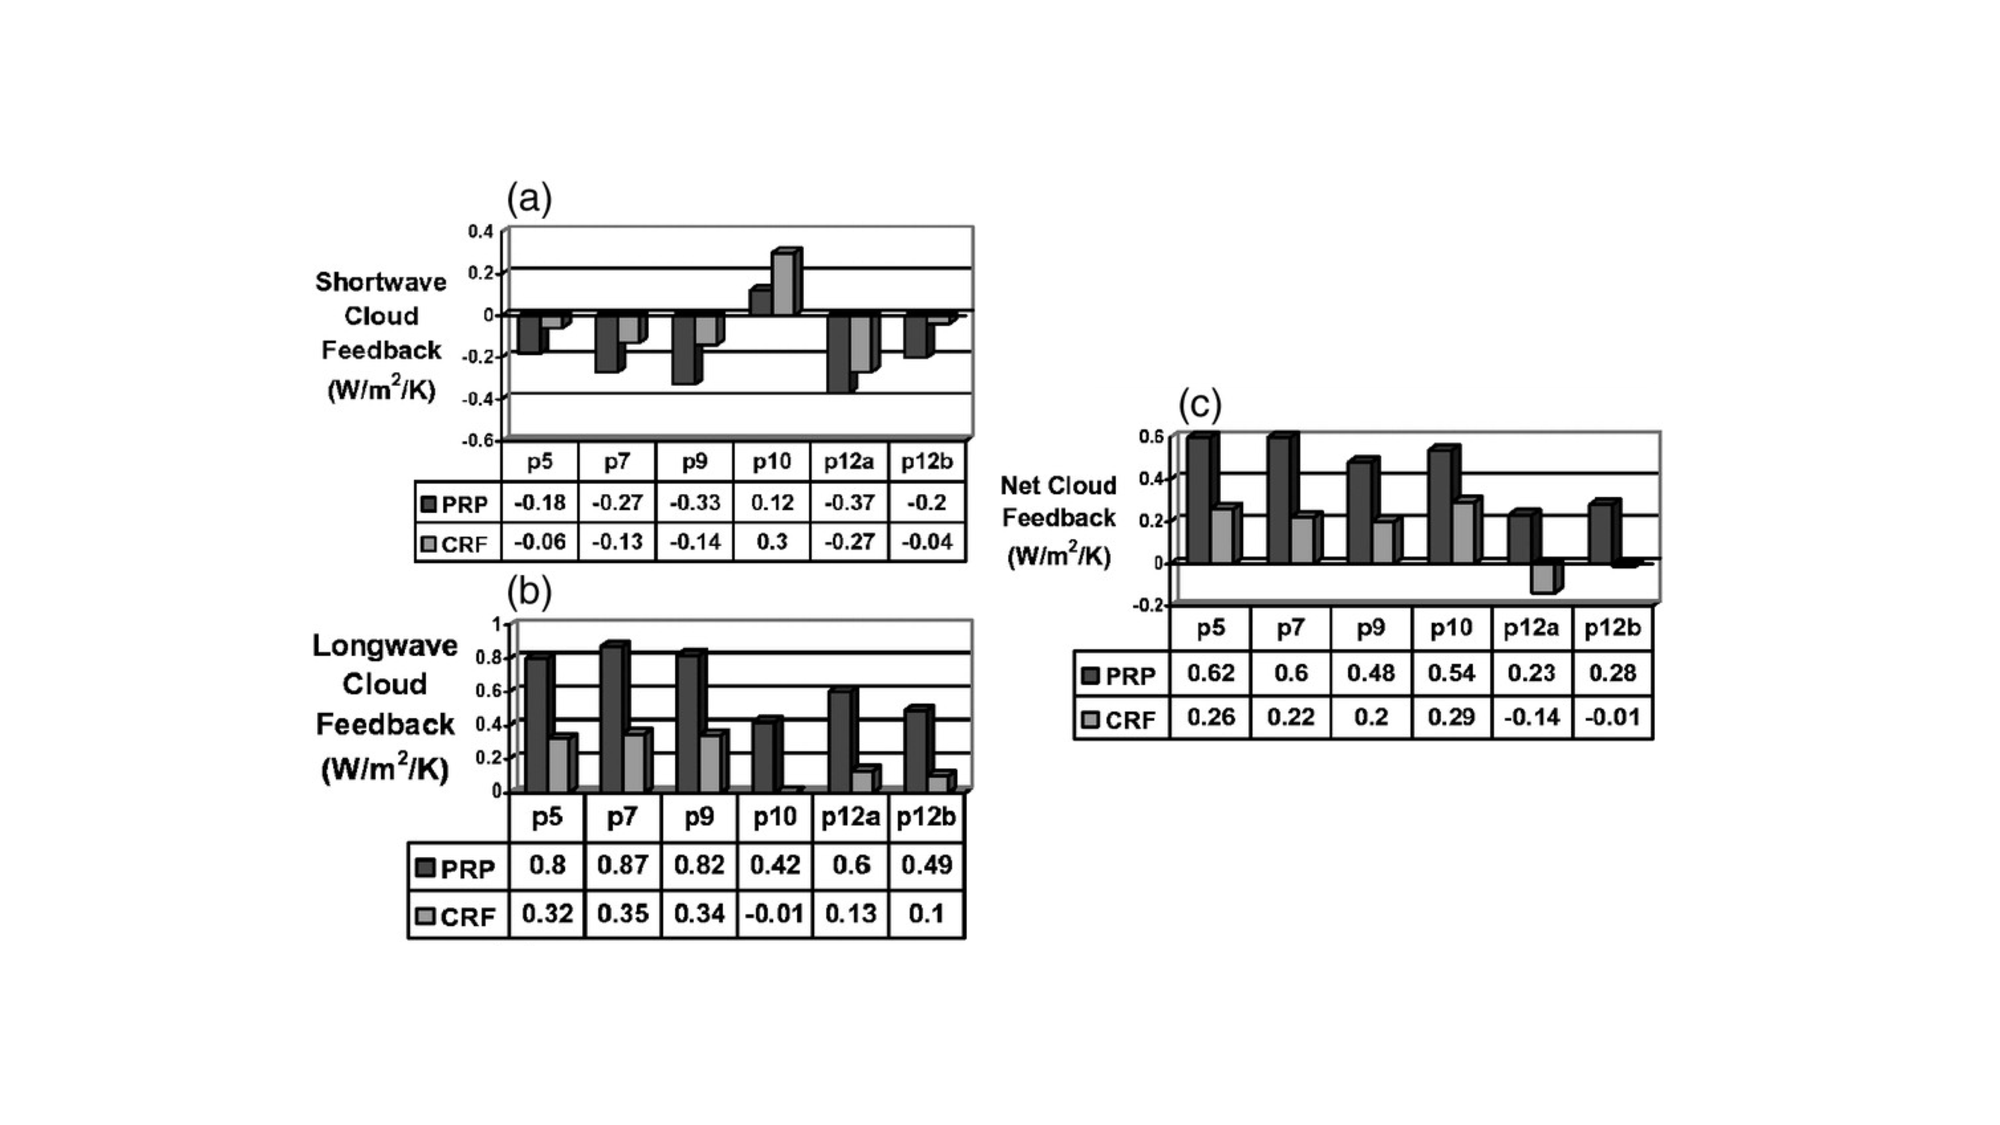
\includegraphics[width=1\linewidth]{{figs/methods/fig2_Soden2004_PRP_CRF_comparison}.pdf}
    \caption{Comparison of the (a) shortwave, (b) longwave, and (c) net cloud feedback parameters from the PRP and $\Delta$CRF (or $\Delta$CRE) methods. Adapted from Fig. 2 of \cite{Soden2004}.}
    \label{fig:cmp_PRP_CRE_Soden}
\end{figure}
If we assume that $\Delta T$, $\Delta w$, and  $\Delta \alpha_s$ are not zero (i.e. $T'\neq T$,  $w'\neq w$, and  $\alpha_s'\neq \alpha_s$), the only way to get $\Delta {CRE}_{net}=0$ would be the changes in total-sky flux (term within first bracket in \eqref{eq:delta_CRE_no_cld_fbk}) and clear-sky flux (term within second bracket in \eqref{eq:delta_CRE_no_cld_fbk}) due to non-cloud feedbacks are equal. However, this is not always the case. An explanation with a simple model is presented in \secref{sec:cld_masking_effect}, but here we provide some simulation results from GCMs first.

Taking the results from \cite{Soden2004} as an example, shortwave (SW), longwave (LW) and net cloud feedback parameters estimated from PRP and $\Delta$CRE mthods from several GFDL AM2 (version numbers denoted as p\#) models are shown in \figref{fig:cmp_PRP_CRE_Soden}. The SW cloud feedback calculated from PRP method is smaller than the ones from $\Delta$CRE method, while the LW cloud feedback from PRP method is larger than that from $\Delta$CRE approach. In total, the magnitude of net cloud feedback from $\Delta$CRE method is underestimated ranges from 0.3 to 0.4 Wm$^{-2}$K$^{-1}$ in AM2 models compared to PRP method. 

\begin{figure}
    \centering
    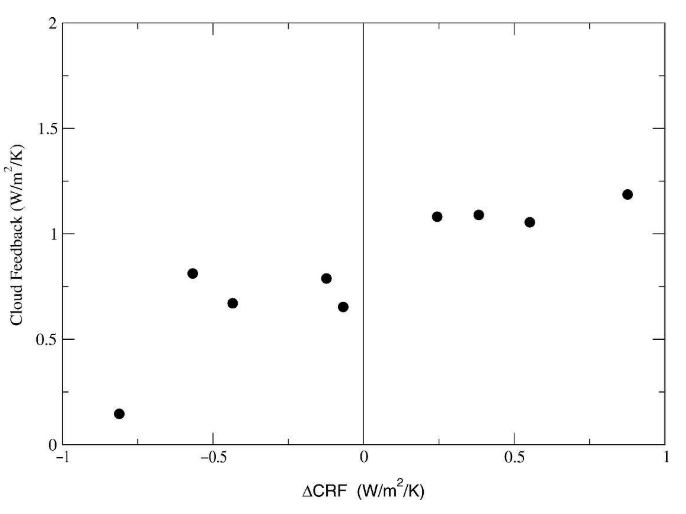
\includegraphics[width=0.65\linewidth]{{figs/methods/Soden_Held_cld_fbk_and_delta_CRF}.png}
    \caption{The cloud feedback parameter plotted as a function of the change in global-mean net cloud radiative forcing per degree change in global surface temperature. Adapted from Fig. 4 of \cite{Soden2006}.}
    \label{fig:cld_fbk_and_CRE_Soden_Held}
\end{figure}

% \begin{figure}
%     \centering
%     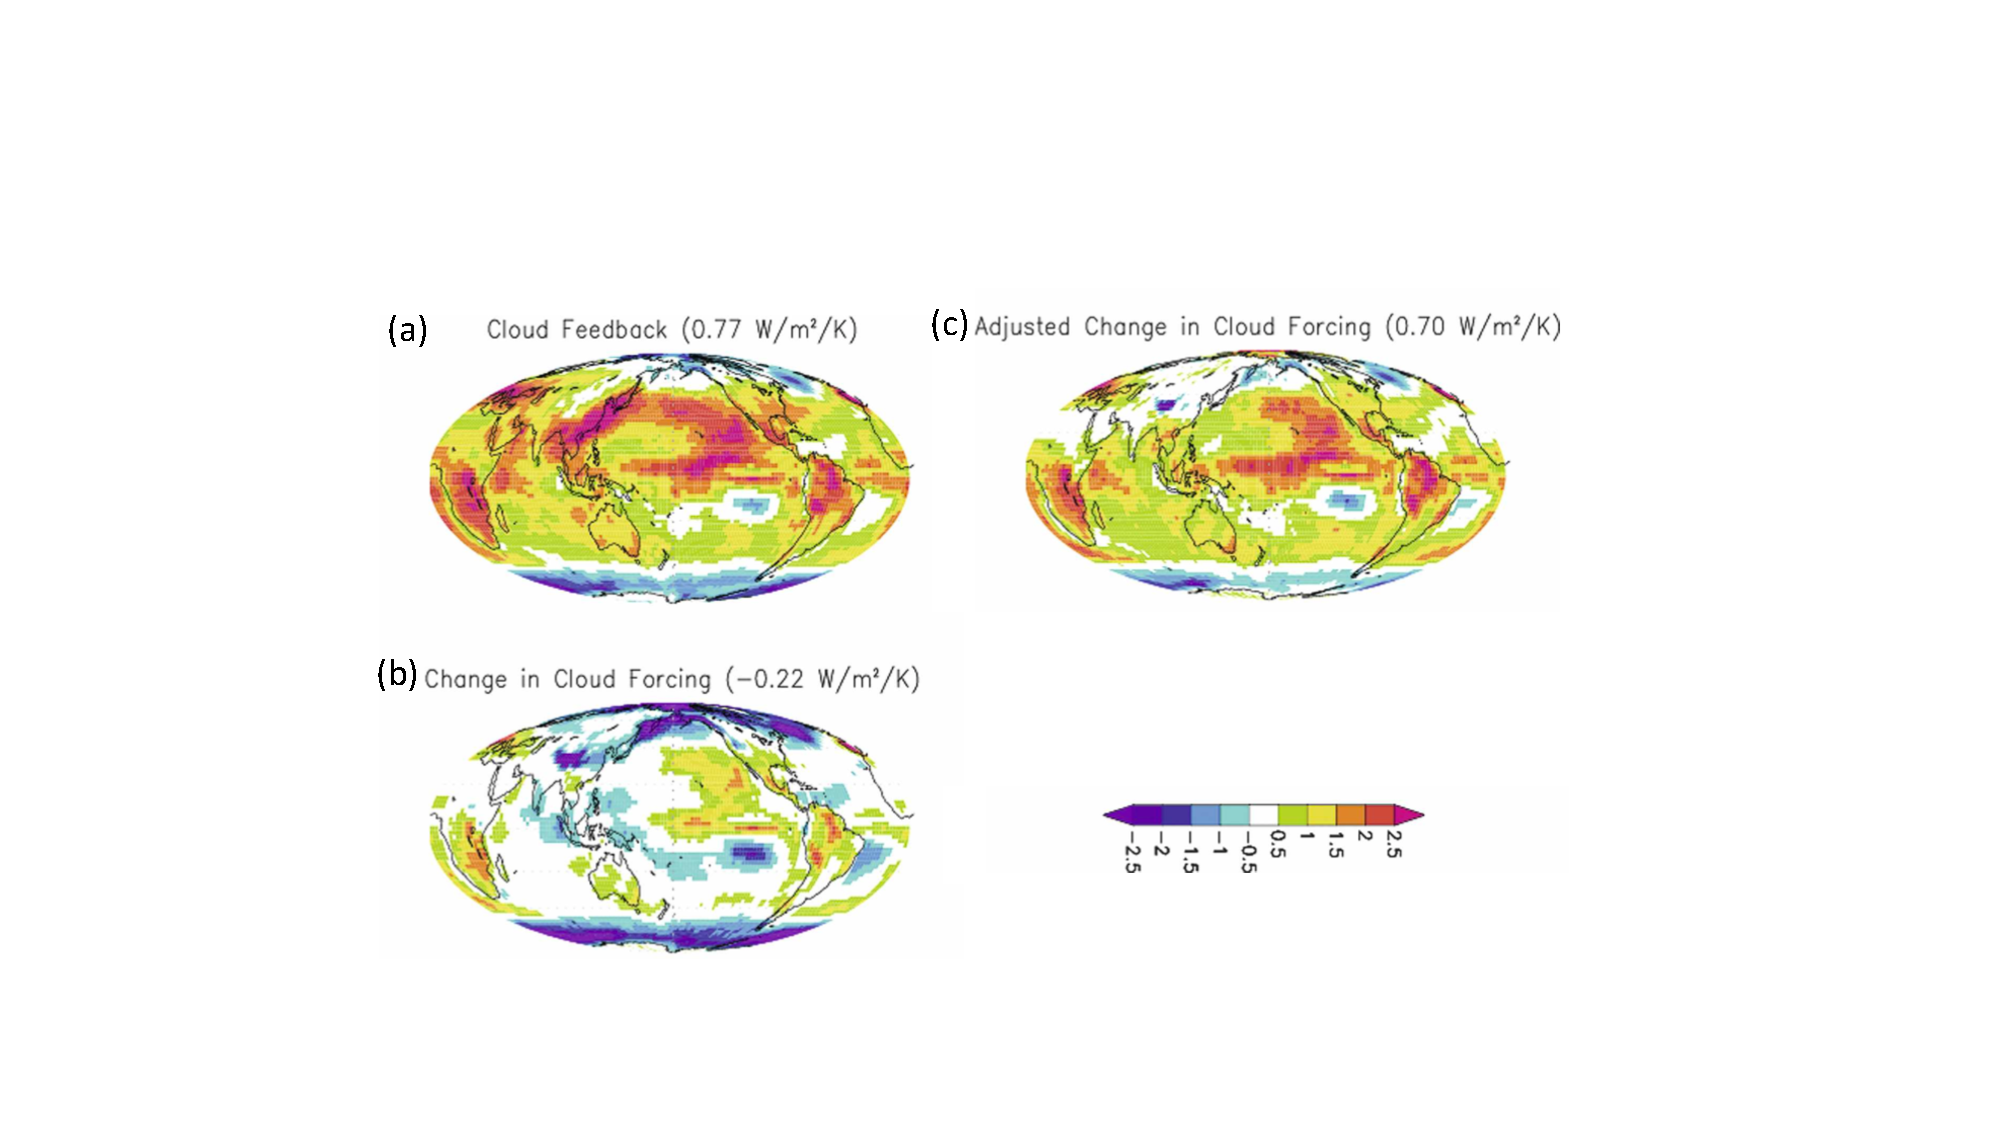
\includegraphics[width=0.9\linewidth]{{figs/methods/cld_fbk_from_kernel_CRF_adjust_forcing}.pdf}
%     \caption{Multimodel ensemble-mean maps of the cloud feedback estimated as (a) the residual of the kernel calculations, (b) the change in cloud forcing, and (c) the change in cloud forcing after adjusting for the effects of cloud masking on noncloud feedbacks and external radiative forcing. Both the cloud feedback and cloud-masking adjustments to the change in cloud forcing are estimated using the GFDL kernel. Adapted from Fig. 11 of \cite{Soden2008}.}
%     %  Only those models for which both the cloud feedback and CRE were available are included in the ensemble mean.
%     \label{fig:cld_fbk_and_CRE_pattern}
% \end{figure}

Similarly, as shown in \figref{fig:cld_fbk_and_CRE_Soden_Held}, \cite{Soden2006} found that all the models from IPCC Fourth Assessment (AR4) have a positive cloud feedback in 21-century climate change experiments, but roughly half the models show a reduction in net CRE (or CRF; and normalized by surface temperature change) in response to climate change. In their study the cloud feedback is estimated by the radiative kernel method. This apparent discrepancy is possibly due to the influence of noncloud feedbacks on the CRE term \citep{Zhang1994,Soden2004}. Therefore, the change of net CRE is not a reliable measure of cloud feedback, as the signs of them are sometimes different (\figref{fig:cmp_PRP_CRE_Soden}c and \figref{fig:cld_fbk_and_CRE_Soden_Held}). However, it is noted that the cloud feedback is correlated with the change in net CRE as displayed in \figref{fig:cld_fbk_and_CRE_Soden_Held}, indicating that intermodel differences in cloud feedback can be estimated by the intermodel differences in the changes of CRE \citep{Soden2006,Bony2006}. %In addition, the spatial patterns of cloud feedback from radiative kernel and $\Delta$CRE approaches are similar, although the magnitude shows large difference (\figsref{fig:cld_fbk_and_CRE_pattern}b and \ref{fig:cld_fbk_and_CRE_pattern}c), implying that the $\Delta$CRE method is still valuable to have a quick look of the cloud feedback pattern.

\subsection{Cloud masking effect}
\label{sec:cld_masking_effect}

A modified simple thought experiment from \cite{Soden2008} is adopted here to explain what cloud masking effect is and why the two right-hand terms in \eqref{eq:delta_CRE_no_cld_fbk} are usually not equal with each other. As illustrated in \figref{fig:cld_masking_effect}, we assume part of the grid is covered by high clouds (cloud fraction is $f$), and the water vapor contents are $q_1$ and $q_2$ for clear and cloudy subgrid regions, respectively. Here we focus on LW radiation only and assume the LW radiation emitted by water vapor is a linear function of its content, that is $\alpha + \beta q$, where $\alpha$ and $\beta$ are assumed linear coefficients and $\beta$ is negative so that the outgoing LW radiation decreases with the increase of water vapor. The outgoing LW radiation emitted from clouds is regarded as a constant $W$.

\begin{figure}
    \centering
    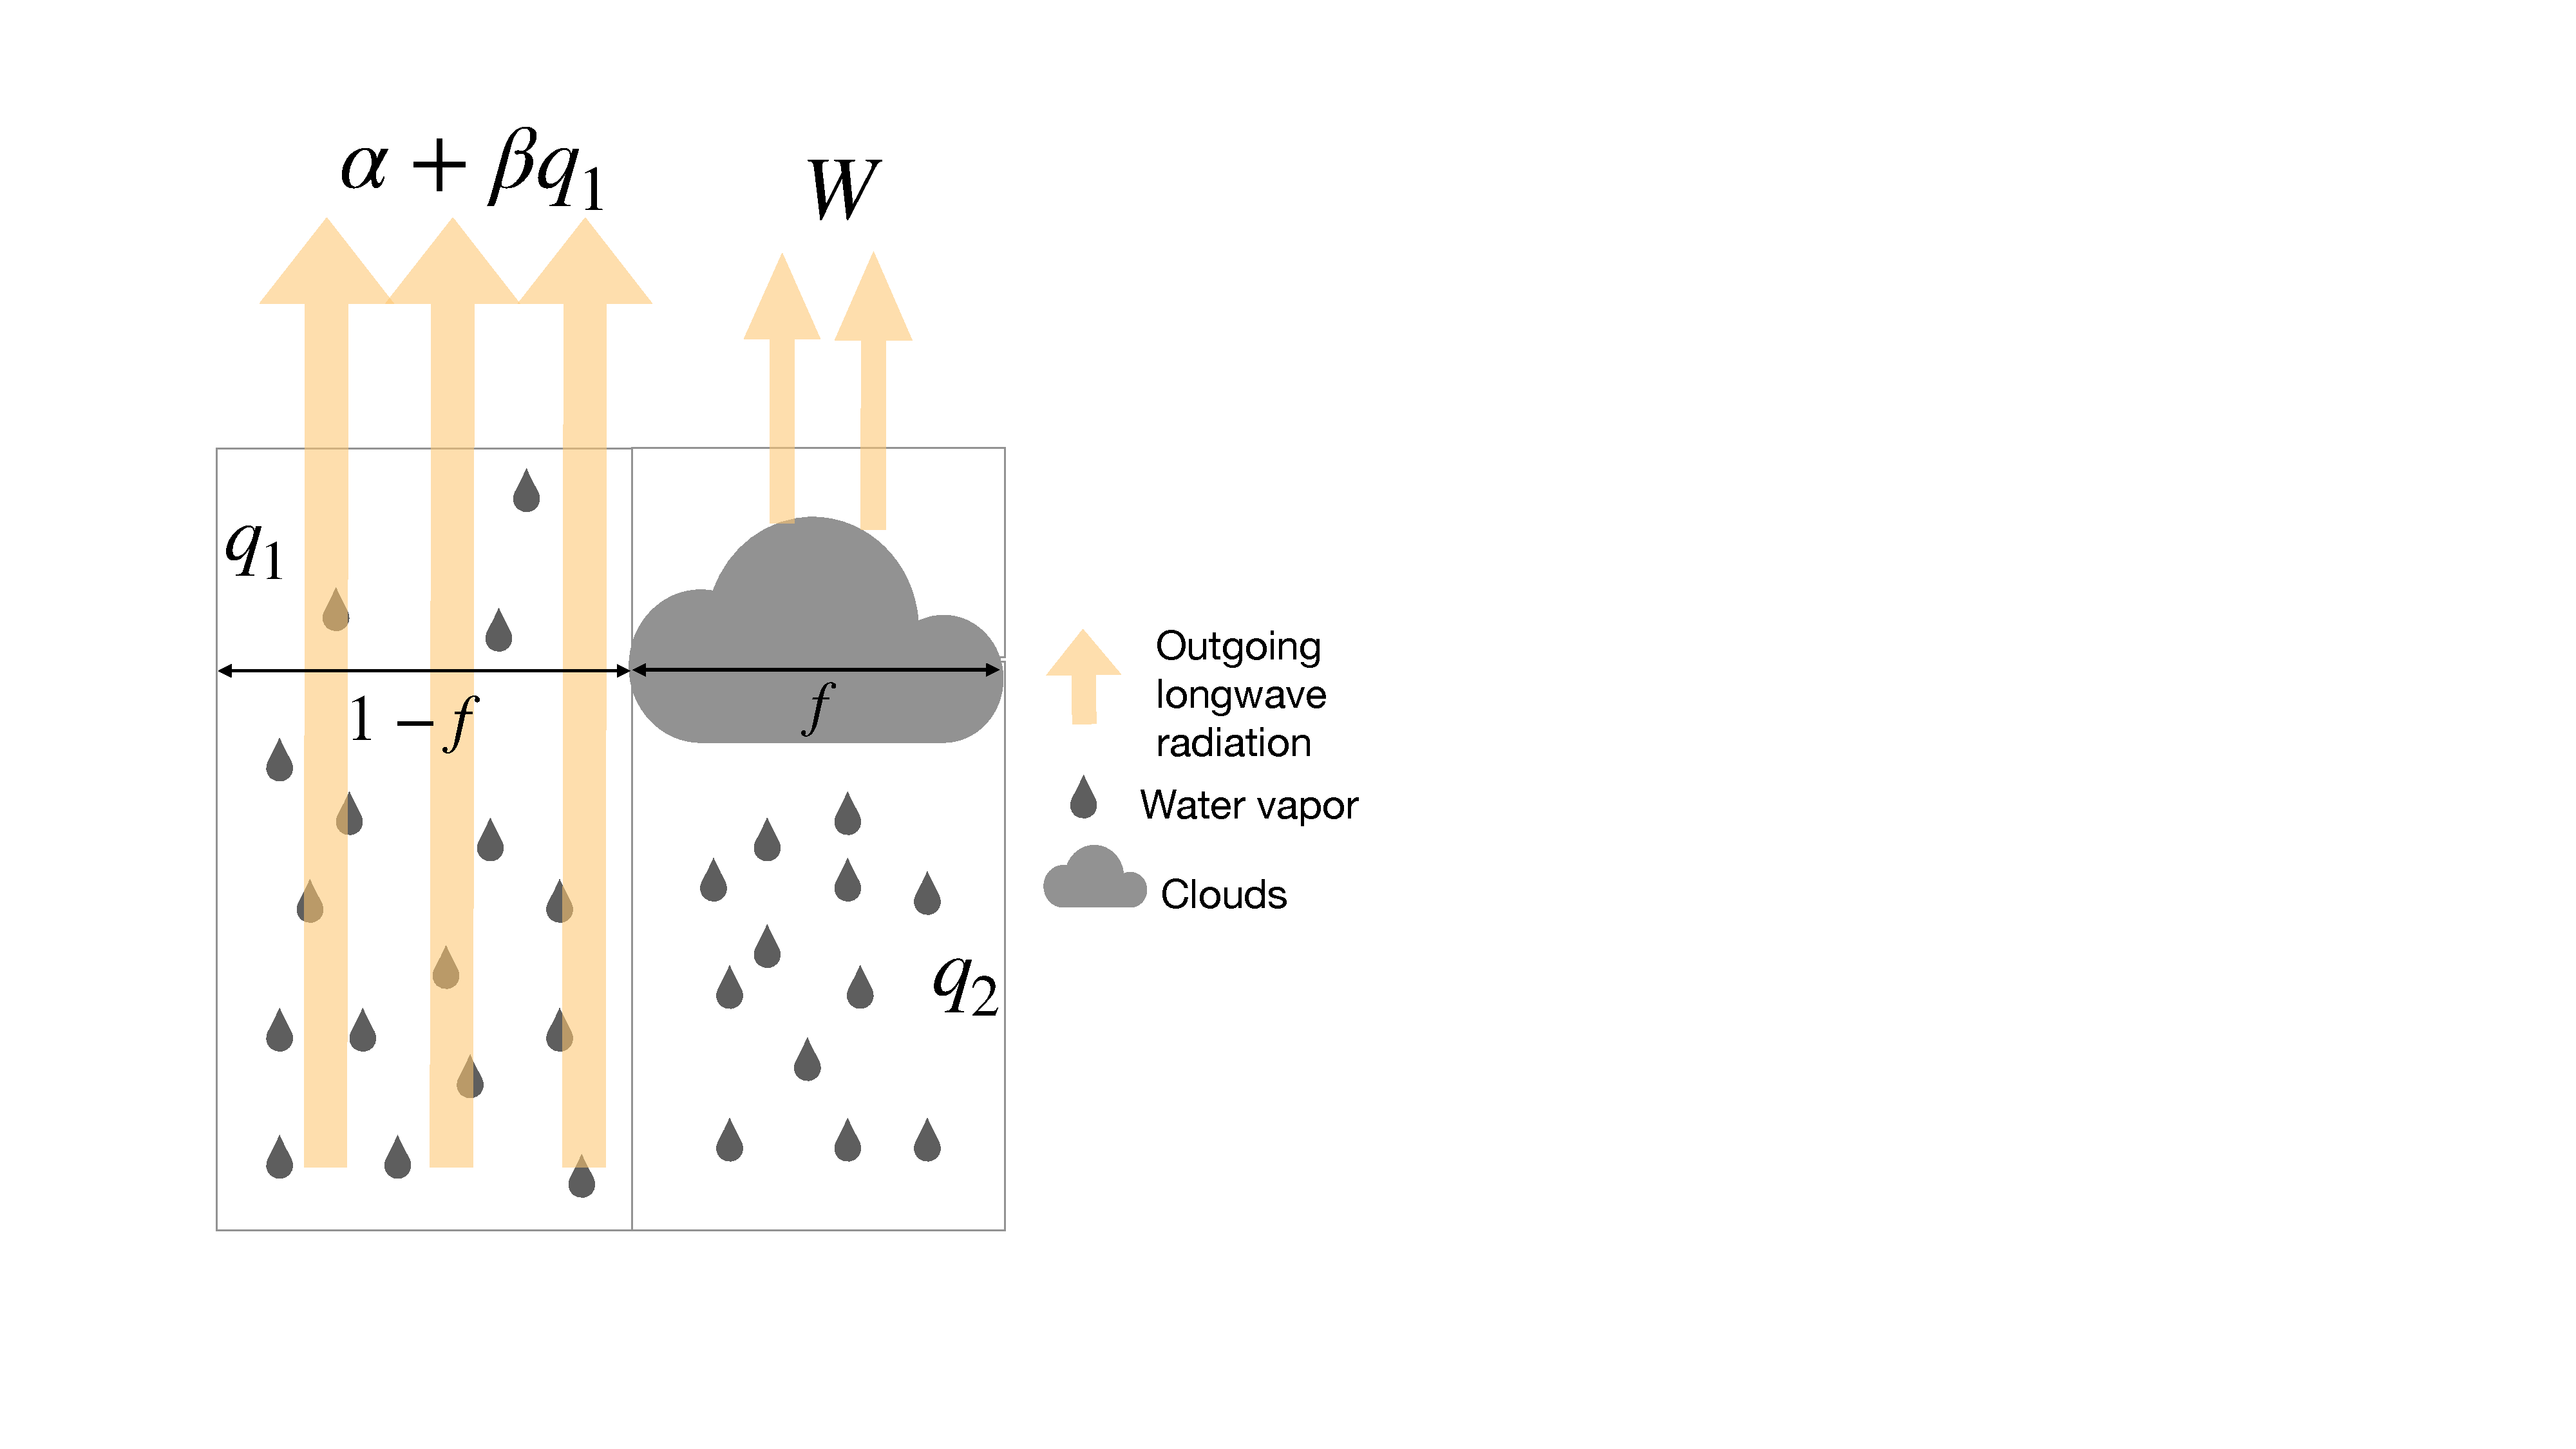
\includegraphics[width=0.65\linewidth]{{figs/methods/cloud_masking_effect}.pdf}
    \caption{Illustration of cloud masking effect on noncloud feedbacks in a grid box.}
    \label{fig:cld_masking_effect}
\end{figure}

If there is no clouds in this grid (i.e. $f=0$), the net LW radiation flux at TOA (downward positive) is $-[\alpha + \beta(q_1+q_2)]$. When clouds are present, the grid averaged net LW flux at TOA becomes
\begin{equation}
    R = - (\alpha + \beta q_1)(1-f)- Wf,
    \label{eq:cld_masking}
\end{equation}
as the LW raditation emitted from water vapor $q_2$ is masked by clouds. Consider a climate change case in which the water vapor and cloud fraction change a bit, and the change in $R$ can be written as follows by differencing \eqref{eq:cld_masking}:
\begin{equation}
    \delta R = \delta R_f + \delta R_q,
\end{equation}
where
\begin{equation}
    \delta R_f = (\alpha + \beta q_1 - W)~\delta f,
    \label{eq:lw_change_due_to_cld}
\end{equation}
and
\begin{equation}
    \delta R_q = -(1-f)\beta~\delta q_1.
    \label{eq:lw_change_due_to_q}
\end{equation}
Now reconsider the situation in \eqref{eq:delta_CRE_no_cld_fbk}, in which there is no cloud feedback ($\delta f=0$), so the LW radiation change at TOA due to clouds is also zero, namely $\delta R_f=0$ in \eqref{eq:lw_change_due_to_cld}. However, as for the  LW radiation flux change due to water vapor perturbation, the cloud fraction $f$ is also included as in \eqref{eq:lw_change_due_to_q}, indicating that clouds have masking effect on the water vapor feedback and the $\delta R_q$ under clear-sky should be different from the one under cloudy condition. 

This simple thought experiment has illustrated that the presence of clouds can have impact on the radiation associated with noncloud variables. That is why the the two right-hand terms in \eqref{eq:delta_CRE_no_cld_fbk} are usually not equal with each other, and it also implies that estimating cloud feedback from changes of cloud radiative effect is probably not a good option due to the cloud masking effect.

\subsection{Cloud radiative kernel method}
\label{sec:Zelinka_method}
In genreal, previous methods introduced in \secref{sec:three_climate_fbk_methods} can give us an estimate of integrated quantity of cloud feedback. Of course, the method such as PRP and radiative kernel can also generate other types of cloud feedbacks by perturbing the corresponding properties, but it is usually hard to do so. To solve this problem, \cite{Zelinka2012computing1,Zelinka2012computing2} propose a new technique based on cloud radiative kernel and the histograms of cloud fraction partitioned by CTP and $\tau$, which can easily attribute the contributions of specific types of cloud changes to cloud feedback.

In this method, the cloud kernel $K$ in each histogram bin of \figref{fig:cld_rad_kernel_Zelinka} is defined as
\begin{equation}
    K = \frac{\partial R}{\partial C},
\end{equation}
which quantifies the sensitivity of TOA radiative flux to cloud fraction changes ($\Delta C$), and is estimated offline from radiation transfer code for each CTP-$\tau$ bin. The process is complicated and detailed description can be found from \cite{Zelinka2012computing1}. The LW, SW and net cloud radiative kernel results are shown in \figref{fig:cld_rad_kernel_Zelinka}, and the major features are:
\begin{enumerate}
    \item The LW cloud radiative kernel is positive for all bins, as the LW CRE is positive. It increases dramatically with cloud top height, and is small near surface as the cloud top temperature contrast with surface is small.
    \item The SW cloud radiative kernel is negative for all bins, as the SW CRE is negative. Its magnitude increases dramatically with optical depth, and almost insensitive to cloud top height.
    \item The net cloud radiative kernels for the lower and thicker clouds are negative, as the SW reflection exceeds LW trapping; while for higher and thinner clouds, the net cloud radiative kenrel are positive, as LW trapping exceeds SW reflection.
\end{enumerate}

\begin{figure}
    \centering
    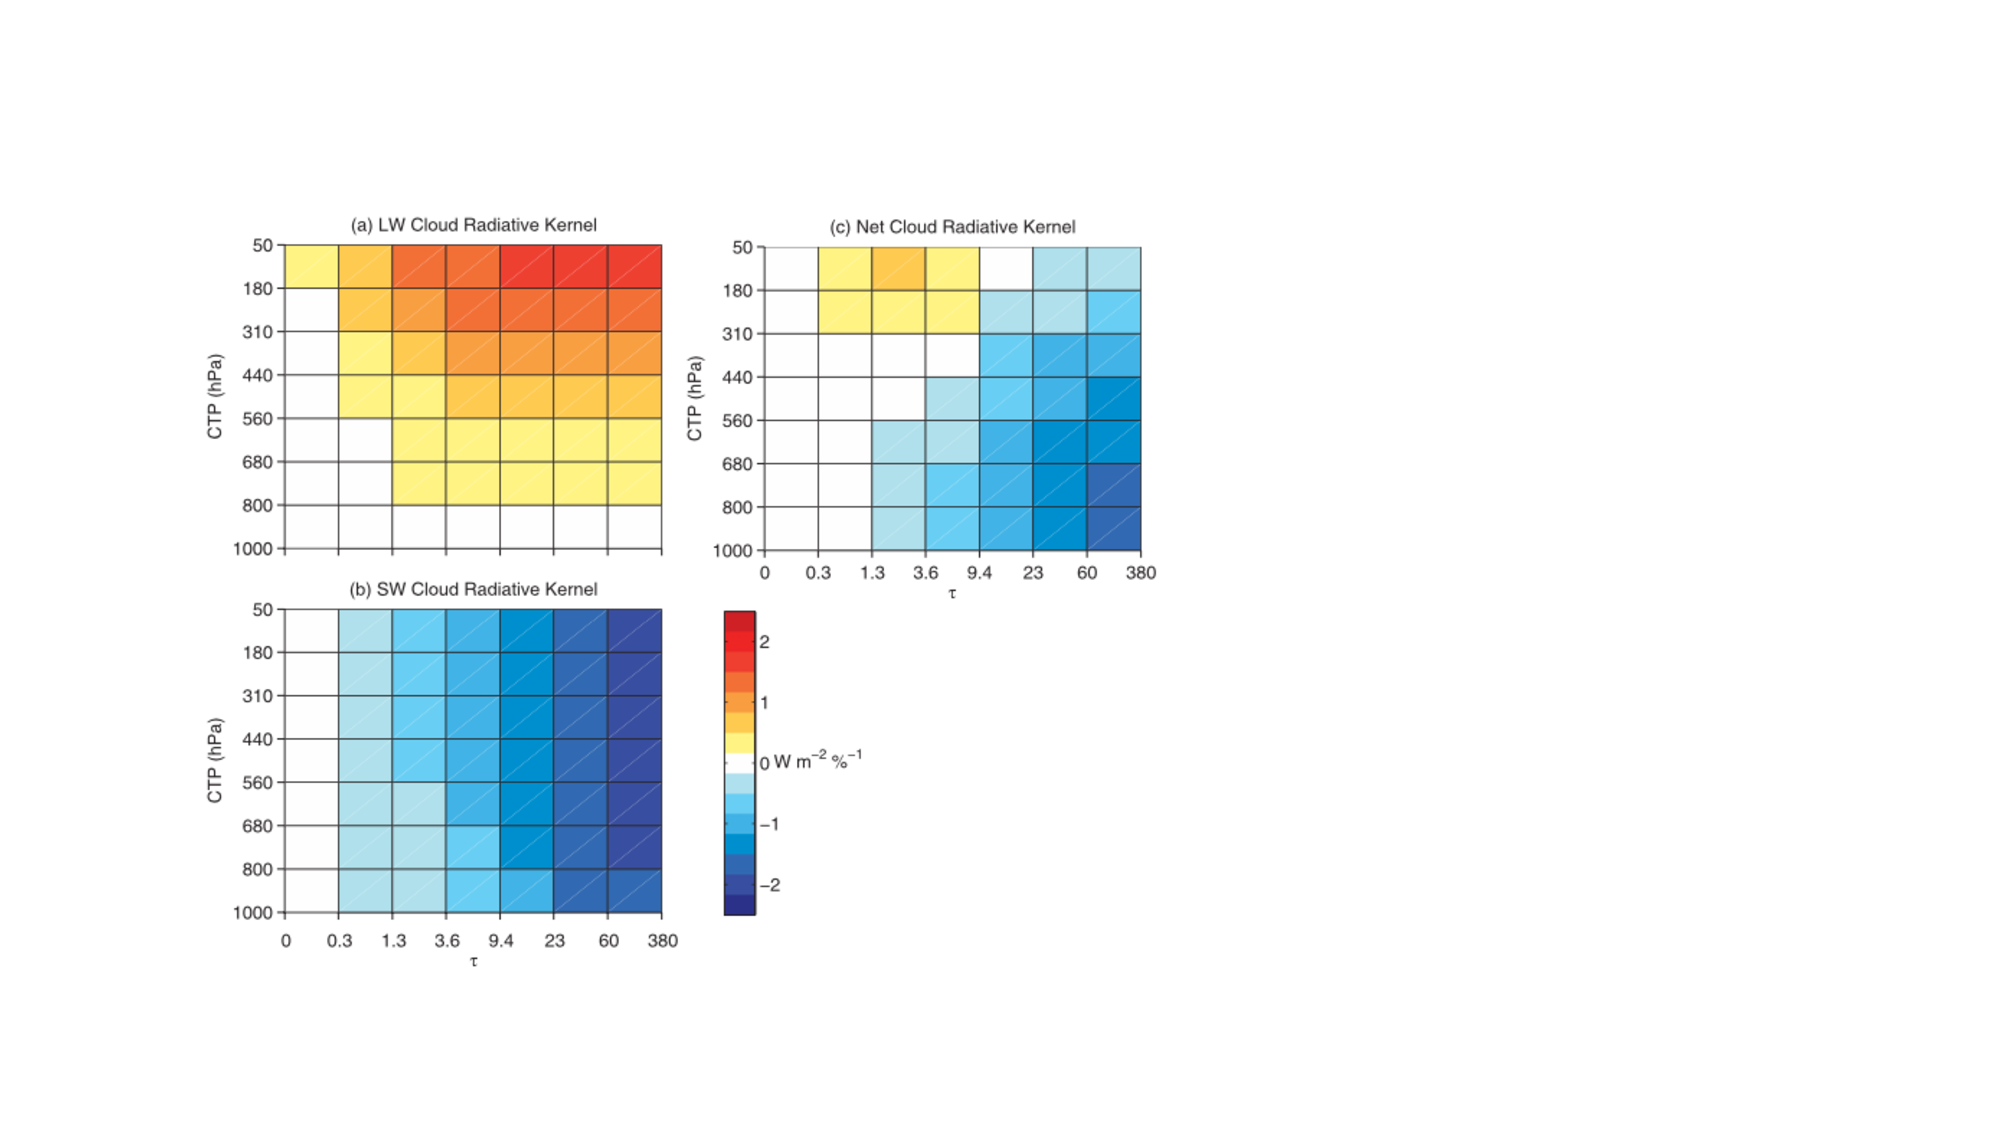
\includegraphics[width=1\linewidth]{{figs/methods/cld_kernel_Zelinka}.pdf}
    \caption{Global, annual, and ensemble mean (a) LW, (b) SW, and (c) net cloud radiative kernels. Adapted from Fig. 1 of \cite{Zelinka2012computing1}}
    % In each model, the kernels have been mapped to the control climate's clear-sky surface albedo distribution before averaging in space; thus, the average kernels are weighted by the actual global distribution of clear-sky surface albedo in each model.
    \label{fig:cld_rad_kernel_Zelinka}
\end{figure}

Multiplying the cloud radiative kernel $K$ by the change in cloud fraction histogram ($\Delta C$, differencing the histogram outputs from cloud simulator) can estimate the contribution of each cloud type to the change in TOA radiation associated with climate change:
\begin{equation}
    \Delta R = K \Delta C
\end{equation}
and hence the cloud feedback is calculated as follows:
\begin{equation}
    \lambda_c = K \frac{\Delta C}{\Delta T_s} = \frac{\Delta R}{\Delta {T}_s}.
\end{equation}
Note that the $\Delta R$ and cloud feedback paramter $\lambda_c$ are function of CTP, $\tau$, latitude, longitude and time, so it can be used to estimate cloud feedback from certain cloud types (according to CTP and $\tau$).


\section{Low cloud amount proxy}

\subsubsection{Low-tropospheric stability}

\cite{Klein1993} studied the seasonal cycle of low stratiform clouds with the data from the Earth Radiation Budget Experiment and found that the low-tropospheric stability (LTS) has a good linear relationship with the low stratus amount, which is applied in Community Atmosphere Model \citep{Collins2004}. In the scheme, LTS can be seen as a measure of the inversion strength and is defined as the potential temperature difference between 700 hPa ($\theta_{700}$) and surface ($\theta_s$),
\begin{equation}
	LTS=\Delta \theta \equiv \theta_{700} - \theta_s.
\end{equation}

\subsubsection{Estimate inversion strength}

\begin{figure}
    \centering
    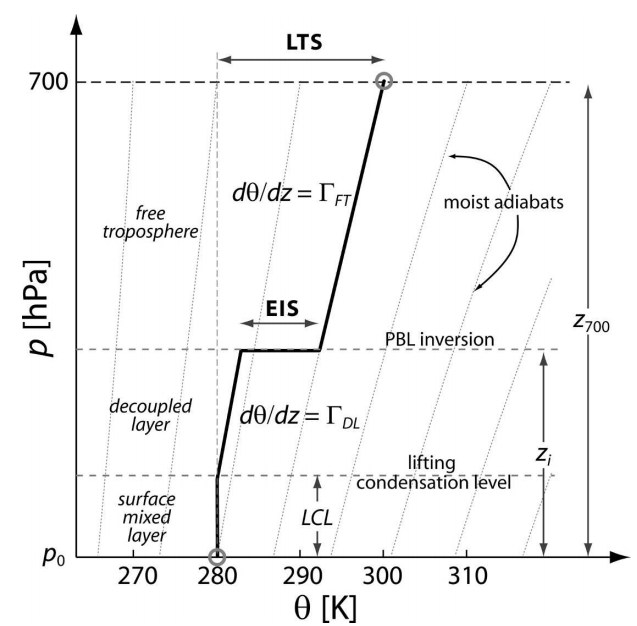
\includegraphics[width=0.8\linewidth]{{figs/methods/Wood_EIS}.png}
    \caption{Idealized profile (thick solid line) of lower-tropospheric structure during periods of undisturbed flow. Moist adiabats are shown as light dotted lines. Adapted from \cite{Wood2006}.}
    \label{fig:wood_eis_atm_profile}
\end{figure}

Despite the widely use of LTS in climate models, \cite{Wood2006} argued that it has yet to be demonstrated
whether the observationally derived LTS-CF relationships will hold in a changed climate. They proposed a new proxy called estimate inversion strength (EIS) to represent the planetary boundary
layer inversion strength and proved that it is better to indicate the low stratiform cloud cover. An idealized profile of lower-tropospheric structure is shown by a thick solid line in Figure \ref{fig:wood_eis_atm_profile}, where the atmospheric conditions roughly follow a dry adiabat below the lifting condensation level (LCL), and then a moist adiabat above. The EIS is defined as
\begin{equation}
    EIS=LTS-\Gamma_{m}^{700} z_{700}+\Gamma_{m}^{LCL} z_{LCL},
    \label{eq:eis}
\end{equation}
or simplified as
\begin{equation}
    EIS=LTS-\Gamma_{m}^{850}\left(z_{700}-z_{LCL}\right),
\end{equation}
where 
\begin{equation}
    \Gamma_{m}(T, p)=\frac{g}{c_{p}}\left[1-\frac{1+L_{v} q_{s}(T, p) / (R_{a} T)}{1+L_{v}^{2} q_{s}(T, p) / (c_{p} R_{v} T^{2})}\right],
    \label{eq:gamma_m}
\end{equation}

\begin{equation}
	z_{700}=\frac{R_{a} T_{0}}{g} \ln \left(\frac{p_{0}}{700~ \mathrm{hPa}}\right).
	\label{eq:z700}
\end{equation}
In \Eqref{eq:eis}, $\Gamma_{m}$ is the moist-adiabatic potential temperature gradient, $z_{700}$ is the height of 700 hPa, $z_{LCL}$ is the height of the lifting condensation level. In \Eqref{eq:gamma_m}, $L_v=2.47\times 10^6$ J kg$^{-1}$ is the latent heat of vaporization. $q_s(T,p)$ is the saturation mixing ratio, and is a function of temperature and pressure derived from the Clausius-Clapeyron equation. $R_a=287.04$ J kg$^{-1}$ K$^{-1}$ and $R_v=461.50$ J kg$^{-1}$ K$^{-1}$ are the gas constants
for dry and water vapor, respectively, $g=9.8$ kg m$^{-2}$ is the gravitational acceleration, and $c_p=1005.0$ J kg$^{-1}$ K$^{-1}$ is the specific heat of air at constant pressure. In \Eqref{eq:z700}, $T_0$ and $p_0$ (in units of hPa) are the surface temperature and pressure respectively.

\subsubsection{Estimated cloud-top entrainment index}

The recent proposed predictors of low cloud amount are also considered in this study: one is the estimated cloud-top entrainment index (ECTEI) by \cite{Kawai2017} and the other is the estimated low-level cloud fraction (ELF) by \cite{Park2019}. 

The ECTEI is a modification of estimated inversion strength (EIS) and takes into account a cloud-top entrainment criterion and is defined as
\begin{equation}
    \mathrm{ECTEI} \equiv \mathrm{EIS} - \beta\left(L_v / c_{p}\right)\left(q_{surf}-q_{700}\right),
    \label{eq:ectei_Kawai}
\end{equation}
where
\begin{equation}
    \beta=(1-k) C_{q\_gap}.
\end{equation}
In \Eqref{eq:ectei_Kawai}, $L_v$ is latent heat of vaporization, and $c_p$ is the specific heat of air at constant pressure. The values of both parameters are the same as the ones in  \Eqref{eq:gamma_m}. $q_{surf}$ and $q_{700}$ are the specific humidity at surface and 700 hPa respectively. The coefficient $C_{q\_gap}$ is the ratio of the total water specific humidity ($q_t$) gap at
the inversion and the $q$ difference between the surface
and 700 hPa. \cite{Kawai2017} estimated the $C_{q\_gap} = 0.76, k=0.70 $ and $\beta = 0.23$ based on radiosonde observation data off the coast of Peru. 
\cite{Park2019} argued that the use of LTS and EIS as a global proxy for low cloud amount is limited
due to their weaker and inconsistent relationship with low cloud amount over land. They kept the calculation of height of inversion, the term with which was neglected in the derivation of EIS \citep{Wood2006}. 
% %\chapter{Simple Experiments Under Isca Framework}
\chapter{The Role of Climate Feedbacks in Polar Amplification}
\label{ch:polaramplification}

%\epigraph{\textit{"Essentially, all models are wrong, but some are useful."}\\ \textit{George Box}, 1987}{}
%\epigraphhead[70]{ \epigraph{\textit{"Essentially, all models are wrong, but some are useful."}}{\textit{George Box}, 1987 } }

\section{Introduction}

% \subsection{Isca model}

% Isca\index{Isca} is an open-source framework for the idealized modeling of global circulation of atmospheres, which provides various options for users to setup experiments for their own interests \citep{Vallis2018}. These options include dry and moist models, various convection and radiation schemes, a variety of land/sea configurations and different parameters for other planetary atmospheres. Taking the radiation scheme in the Isca as an example, the choices include two gray radiation schemes (gray means that radiation in different wavelength is treated equally), which we call Frierson \citep{Frierson2006} and Byrne \& O'Gorman \citep[BOG hereafter;][]{Byrne2013}; an intermediate scheme with two infrared bands and one solar band, similar to \cite{Geen2016}; and a full radiation scheme, the multiband correlated-$k$ Rapid Radiative Transfer Model \citep[RRTM;][]{Clough2005}. In fact, the plentiful options in the Isca offer users an opportunity to explore the models with different levels of complexity under the same framework.

% %\citealp{Clough2005}
% %In addition, the Isca model provides a python wrapper for the model to configure and run the experiments easily. 
% %it is to provide a means whereby a complex system may be easily modelled in different ways, with different levels of complexity, thus providing a nearly continuous pathway from comprehensive numerical modelling to conceptual modelling and theory for Earth and planetary atmospheres (Isca paper)

% However, there are no interactive cloud schemes, dynamical ocean and sophisticated land-surface models in the Isca currently, compared to the comprehensive climate models. In general, clouds associated with weather and climate phenomena are the essential parts of the climate system, but the simulations of clouds and their feedbacks have large uncertainties in current general circulation models (GCMs). For example, as pointed by \cite{Ceppi2017}, cloud feedback\index{cloud feedback} is the largest source of intermodel spread in equilibrium climate sensitivity in the recent Climate Model Intercomparison Project phase 5 (CMIP5). Therefore, it is very important to understand clouds and their feedback to the climate systems. Generally, the models are supposed to be as close to the nature as possible for the real simulation results, which will, however, lead to the situation in which the models sometimes are too complicated to fully understand. In this case, it is of great help to employ the simple models to investigate the key mechanisms behind the various phenomena. In this chapter, we will make use of Isca to design some simple experiments investigating the zonal mean surface temperature change especially polar amplification of surface temperature change in aquaplanet simulations.%polar amplification of surface temperature change.

% %One dilemma situation for models is that they have to be as close to nature as possible to get real simulation results, which, however, results in that the models are sometimes too complicated to fully understand. 

% %In other words, the aim of my PhD project is to investigate the roles of clouds in the climate system by building simple cloud schemes within Isca model. 
 
% \subsection{Polar amplification}

Polar amplification\index{Polar amplification} is the phenomenon where surface temperature in the polar regions rises faster than the global average \citep{IPCC2007Synth,Stocker2013}, which exists not only in observation where Arctic warming is evident \citep{Johannessen2004,Polyakov2002}, but is also confirmed by models at varying levels of complexity \citep[e.g.,][]{Winton2006amplified,Langen2007,Merlis2018,Alexeev2005}.

Many discussions have focused on the sea ice and surface albedo feedback\index{Feedback!surface albedo} when discussing the mechanisms of polar amplification under global warming, as it is obvious that initial warming will melt the sea ice in Arctic region, leading to the decrease of surface albedo, which in turn will lead to the absorption of more solar radiation and cause the further retreat of sea ice cover \citep{Serreze2011}. In fact, diminishing sea ice does play a leading role in recent Arctic temperature amplification \citep{Screen2010}. Nevertheless, polar amplification also occurs in simulations even without sea ice and surface albedo feedbacks \citep[e.g.,][]{Alexeev2005,Langen2012,Cai2005,Cai2006}. Different physical mechanisms have been proposed to explain polar amplification, including increasing northward heat transport \citep{Alexeev2005} and climate feedbacks such as Planck feedback\index{Feedback!Planck}, lapse rate feedback\index{Feedback!lapse rate}, cloud feedback and water vapor feedback\index{Feedback!water vapor} \citep{Pithan2014,Screen2010,Vavrus2004}. In addition, these mechanisms will interact with each other in the climate system, making the quantification of the contributions to polar amplification more complicated. For instance, \cite{Graversen2009} found that an increase of water vapor and total cloud cover is favorable for a stronger greenhouse effect in the Arctic than at lower latitudes with fixed albedo under doubled CO$_2$ forcing. However, \cite{Screen2010} find no evidence of changes in cloud cover contributing to recent near-surface Arctic warming.
 
\cite{Goosse2018} categorized the feedbacks in the polar regions into radiative and non-radiative feedbacks, in which the first is linked the surface temperature change to the perturbation of top of the atmosphere (TOA) energy budget and the latter one is associated with sea ice, the ocean and other components of the climate system. In fact, radiative feedback analysis can provide clear insights into the mechanisms of surface temperature change at high latitudes, and thus we focus on radiative feedback analysis only in this study. Besides surface albedo feedback, various feedback processes in the climate system can also contribute to polar amplification. Compared to regions with higher background temperature, a given increase in emitted radiation requires a larger temperature increase at colder regions according to the Stefan-Boltzman law, indicating that Planck feedback\index{Feedback!Planck} (i.e., feedback related to uniform warming in surface and tropsphere) supports polar amplification naturally \citep{Pithan2014}.

The lapse rate feedback\index{Feedback!lapse rate}, associated with vertically non-uniform warming of the atmosphere, is negative in tropical region as the vertical temperature profile is close to moist adiabatic. It is positive in the polar regions due to the larger static stability, leading to `top-heavy' and `bottom-heavy' warming profiles in tropical and polar regions respectively \citep{Graversen2009, Pithan2014, Manabe1975, Kim2018}. As for the water vapor feedback\index{Feedback!water vapor}, the increased water vapor will amplify the greenhouse effect and cause further warming, and is bigger in tropical regions as the increase of water vapor is greater there \citep{Taylor2013, Pithan2014}. In fact, the quantification of the relative importance of these contributions is difficult. For example, \cite{Pithan2014} pointed out that temperature feedback is the largest contribution and surface albedo feedback is the second main contributor to Arctic amplification, which is, conversely, cited as the largest contributor in some studies \citep[e.g.,][]{Manabe1975,Winton2006amplified,Hall2004}.

%About the role of cloud... \cite{Kim2018} also pointed out that.... 

In this chapter, we will revisit the polar amplification problem with a hierarchy of radiation schemes provided in the Isca model \citep{Vallis2018}, in order to investigate the roles of different climate feedbacks. As introduced in \chapref{ch:methods}, the radiation scheme choices include two gray radiation schemes, Frierson \citep{Frierson2006} and Byrne \& O'Gorman \citep[BOG hereafter;][]{Byrne2013}, and the multiband correlated-$k$ Rapid Radiative Transfer Model \citep[RRTM;][]{Clough2005}. In fact, the plentiful options in the Isca offer users an opportunity to explore the models with different levels of complexity under the same framework. For instance, the role of water vapor can be examined closely, as the Frierson and BOG schemes are similar except there is no water vapor feedback in the first scheme (see details in \secref{sec:wv_fb_setup}).

This chapter is structured as follows. \secref{sec:polar_amiplicaiton_setup} describes the experimental setups and lists the details and differences of the two gray radiation schemes used in the simulations. \secref{sec:method_radiative_kernel} quantifies the Planck, lapse rate and water vapor feedbacks from three radiaiton schemes in the Isca through the radiative kernel method, in which the radiative kernels are derived from the offline calculation of radiation codes. In \secref{sec:polar_amiplification_results}, we investigate the roles of heat transport and various climate feedbacks in polar amplification of surface temperature change in the Isca simulations. The conclusions are summarized and discussed in \secref{sec:polar_amplification_summary}.

%With these choices, we can examine some of the mechanisms such as water vapor feedback associated with the polar amplification so as to understand them in further.

\section{Experimental setup}
\label{sec:polar_amiplicaiton_setup}

\subsection{Basic setup}

The Isca model is employed for the simulations. The configuration has 25 vertical levels and is run with a spectral dynamical core at T42 horizontal resolution, roughly equivalent to 2.8 degrees in latitude and longitude. The atmosphere is coupled to a slab ocean with a depth of 10m. The insolation conditions for all the experiments are perpetual equinox without seasonal change but with diurnal variations, because the perpetual equinox insolation can cause the most evident polar amplification compared to the seasonal and annual-mean insolations \citep{Kim2018}. Three radiation schemes (i.e. BOG, Frierson and RRTM schemes) are applied in our experiments to calculate the radiative transfer, as BOG and Frierson schemes are relatively simple gray radiation schemes and RRTM is a widely used full radiation scheme, which can provide a good reference for the results. The sea ice formation is not enabled in the model even if the surface temperature is below the freezing point. Furthermore, the global uniform albedo is adopted in the model, and thus the surface albedo feedback is disabled. The default CO$_2$ concentration is 360 ppm. All the experiments are run for 20 years following 10 years of spinup.
%  Oceanic heat transport is prescribed with symmetric Q-flux with respect to equator. 

%The albedo ($\alpha$) used in our experiment are 0.27, 0.3, 0.33 and 0.38, where $\alpha =0.3$ is used in the control run.

\subsection{Changing forcing through varying albedos}

The general way to investigate climate sensitivity is to evaluate the degree of warming in response to a doubling of the CO$_2$ concentration in the climate system. Actually, the external forcing can be introduced into the climate system through other ways such as adding a ghost forcing  arbitrarily at the TOA \citep{Hansen1997,Alexeev2005}. Given the fact that there is no sea ice in our experiments, changes of albedo will not introduce albedo feedbacks to the climate system. Instead, it provides an simple way to perturb the radiation balance at the TOA without doubling CO$_2$ concentration. Therefore, we will first examine the zonal mean surface temperature change when varying the albedo. Specifically, four albedos, $\alpha=$0.27, 0.3, 0.33 and 0.38, are selected for each radiation scheme in this study, where $\alpha = 0.3$ is roughly the Earth's global averaged albedo and used in the control run for each radiation scheme. $\alpha=0.27$ (0.33) decreases (increases) $10\%$ from the control run value, which will cause the warming (cooling) response to the climate system. $\alpha=0.38$ increases even more than the albedo in the control run, leading to a much colder climate state. The experiments for the BOG, Frierson and RRTM radiation schemes with different albedos are shown in \tabref{tab:exp_table}.

\begin{table}[ht]
	%\setlength\extrarowheight{-3pt}
	\centering
	\caption{The experiments for the BOG, Frierson and RRTM radiation schemes with four different albedos, where $1\times$ indicates the CO$_2$ concentration is not doubled.} % and 2x for the $CO_2 = 720$ppm
	\vspace{0.5em}
	\renewcommand{\arraystretch}{1.3}
	\small
	%\begin{tabular}{|c|*{4}{c|}}
	\begin{threeparttable}
	%\resizebox{0.8\textwidth}{!}{
	\begin{tabular}{c|*{4}{c}}
		\toprule
		%\diagbox{Scheme}{Albedo} & 0.38 &0.33& 0.3$^*$ & 0.27 \\
		\diagbox{Scheme}{Albedo} &\makebox[3em]{0.38}&\makebox[3em]{0.33}&\makebox[3em]{0.3\tnote{*}}
		&\makebox[3em]{0.27}\\
	    \midrule
		%Byrne \& O'Gorman &  $1\times$, $2$x & $1\times$, $2$x & $1\times$, $2$x & $1\times$, $2$x \\
		Frierson & $1\times$ & $1\times$ & $1\times$ & $1\times$ \\ 
		BOG &  $1\times$ & $1\times$ & $1\times$& $1\times$ \\
		RRTM & $1\times$ & $1\times$ & $1\times$ & $1\times$ \\
		\bottomrule
	\end{tabular}%
	\begin{tablenotes}
      \setstretch{1.3}
      \item[*] indicates the control run for each radiation scheme.
     \end{tablenotes}
	\end{threeparttable}
	\label{tab:exp_table}
\end{table}

To estimate the external forcing after changing the albedos, the fixed sea surface temperature (SST) forcing method is applied in this study \citep{Hansen2005,Andrews2012cloud,Feldl2013,Kim2018}, which has included the adjustment throughout the atmosphere. For each radiation scheme, the radiative forcing for experiments after changing albedos ($\alpha=0.27, ~0.33$ and $0.38$) is calculated from radiation imbalance at TOA when prescribed with the monthly mean SST profiles from control experiment.

%As shown in \tabref{tab:exp_table}, the experiments are also performed for the BOG radiation scheme with CO$_2$ concentration doubled to have a reference.
% \begin{figure}[ht]
% 	\centering
% 	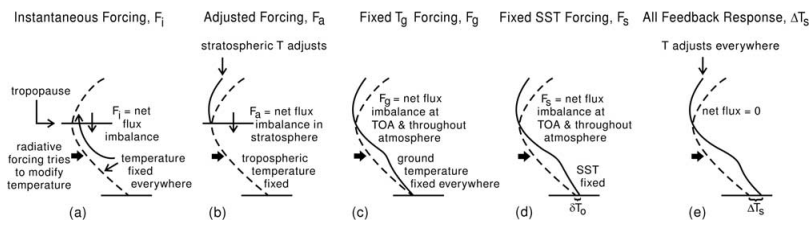
\includegraphics[width=1.0\linewidth]{{figs/polar_amp/Hansen2005_forcings}.png}
% 	\caption{ Cartoon comparing (a) $F_i$, instantaneous forcing, (b) $F_a$, adjusted forcing, which allows stratospheric temperature to adjust, (c) $F_g$, fixed $T_g$ forcing, which allows atmospheric temperature to adjust, (d) $F_s$, fixed SST forcing, which allows atmospheric temperature and land temperature to adjust, and (e) $\Delta T_s$, global surface air temperature calculated by the climate model in response to the climate forcing agent. Adapted from Figure 2 of \cite{Hansen2005}.}
% 	\label{fig:Hansen_forcing}
% \end{figure}

\subsection{Water vapor feedback in radiation scheme}
\label{sec:wv_fb_setup}
%\vspace{-1.6cm}

To examine the roles of water vapor feedback in polar amplification, the BOG and Frierson radiation schemes are employed in this study, as only one of the schemes provides moisture feedback. According to \cite{Byrne2013} and \cite{Frierson2006}, the same shortwave radiation schemes are adopted in both schemes, but the ways to calculate the longwave radiative transfer are different. Specifically, the longwave optical thickness ($\tau$) for the BOG scheme in the Isca is
\begin{equation}\label{eq:bog_tau}
    \frac{\text{d}\tau}{\text{d}\sigma}=a\mu+bq+c~\text{log}(\text{CO}_2/360),
\end{equation}
where $\sigma = p/p_0$, and $p_0$ is $10^3$ hPa; $q$ is the specific humidity and $\mu=1$ is a scaling parameter intended to represent absorption by well-mixed gases; $a=0.1627$, $b=1997.9$ and $c=0.17$ are values recommended in \cite{Vallis2018}. CO$_2=360$ ppm is the default CO$_2$ concentration, which has no effect on changes in longwave optical thickness at this default level. It is evident that water vapor feedback can have an impact on the optical depth in the BOG radiation scheme. However, long-wave optical depth in the Frierson scheme is a function of latitude ($\theta$) and pressure ($p$) \citep{Frierson2006}, which is specified to approximate the effects of atmospheric water vapor. The surface value of optical depth ($\tau_0$) is given in the form of
\begin{equation}\label{eq:frierson_lw_optical_depth1}
\tau_0 = \tau_{0e}+(\tau_{0e}-\tau_{0p})\operatorname{sin}^2\theta,
\end{equation}
where $\tau_{0e}$ and $\tau_{0p}$ are the surface optical depth at equator and pole separately. The vertical structure of optical depth ($\tau$) is a combination of a linear term, which is included to reduce stratospheric relaxation times, and a quartic term, which is used to approximate the structure of water vapor in the atmosphere as it is an absorber with a scale height that is one quarter of the density-scale height, and thus is given by
\begin{equation}\label{eq:frierson_lw_optical_depth2}
\tau=\tau_0\left[f_l\frac{p}{p_s}+(1-f_l)\left(\frac{p}{p_s}\right)^4\right],
\end{equation}
where $p_s$ is sea level pressure and coefficient $f_l$ is set to 0.1 in the equation. Note that moisture is held fixed in the Frierson scheme, which implies that the comparison between simulation results from BOG and Frierson schemes can demonstrate the role of water vapor feedback in polar amplification. To investigate that role in further, we re-run the experiments for the BOG scheme without allowing water vapor feedback by prescribing the annual and zonal mean specific humidity profiles from the control run. In this case, the processes such as water vapor advection and convection will carry on as usual, but the moisture feedback is turned off. All the associated results will be shown in \secref{sec:polar_amiplification_results}.

%where $p_s$ is sea level pressure and the linear term ( $f_l$ is 0.1 in the equation). The quartic term is used to approximate the structure of water vapor in the atmosphere as scale height of water vapor is roughly $1/4$ of the density-scale height, but the optical thickness is fixed for each latitude and pressure level, implying that there is no moisture feedback in the Frierson radiation scheme. Therefore, the comparison between simulation results from BOG and Frierson schemes could show the significance of water vapor feedback in polar amplification. To investigate the role of water vapor feedback in polar amplification in further, we re-run the experiments for the BOG scheme without allowing water vapor feedback by prescribing the annual and zonal mean specific humidity profiles from the control run. Therefore, the processes such as water vapor advection and convection will carry on as usual in the BOG scheme, but the optical depth is fixed and the moisture feedback is turned off. The associated results will be shown in \secref{sec:results}.

%we write out specific humidity ($q$) from experiment where the albedo is 0.3 for the BOG scheme, and then the annual and zonal mean $q$ profile will be read back into the BOG scheme for all the runs with four different albedos. 

%Write the zonally and time averaged specific humidity ($q$) into file from experiment where the albedo is 0.3.
%Read $q$ back into the BOG radiation scheme in all the runs.
%The $q$ only written into the radiation scheme not other parts of the model, which is used to fix the optical depth when altering the albedos. 
%\subsection{Roles of water vapor feedback and CO$_2$}

%%%%%%%%%%% ------------------ Section ------------ %%%%%%%%%%%%%
%\section{Method}
\section{Quantify climate feedbacks in Isca}
\label{sec:method_radiative_kernel}

\subsection{Introduction}

In order to quantify the relative importance of various contributions to polar amplification, the radiative kernel technique \citep{Soden2008,Shell2008} is used to calculate various climate feedbacks (see \secref{sec:rad_kernel_method_for_pa}). In general, climate feedback is used to characterize the response of the climate system to an external radiative forcing, which can either amplify or diminish the effect of the forcings \citep{Hansen1984}. The change of net radiative flux at TOA between two different climate states, $\Delta R$, can be represented by
\begin{equation}
    \Delta R = \Delta F+\lambda \Delta T_s + \mathcal{O}\left( \Delta T_s^2 \right),
\label{eq:delta_R_relation}
\end{equation}
which can be viewed as a Taylor expansion in surface temperature change ($\Delta T_s$) \citep{Feldl2013a}. The first term, $\Delta F$, in \Eqref{eq:delta_R_relation} is the climate forcing, which is estimated by the fixed-SST method \citep{Hansen2005,Feldl2013a,Kim2018}. The second term, $\lambda \Delta T_s$, reflects the radiative flux change that is linearly dependent on the surface temperature change, and $\lambda$ is the total \textit{feedback parameter}. The third term (or residual term) $ \mathcal{O}\left(\Delta T_s^2 \right)$ represents the high-order components, reflecting the non-linear interactions among different processes, which we consider to be neglected in our analysis. It should be pointed out that variables in \Eqref{eq:delta_R_relation} can be a global mean value or a function of the latitude \citep{Feldl2013a}. When neglecting the nonlinearities and interactions among the feedbacks, the feedback parameter $\lambda$ can be decomposed into the sum of different components:
\begin{equation}
\lambda=\lambda_T+\lambda_{w} +\lambda_\alpha+\lambda_C,
\label{eq:fb_decmop}
\end{equation}
where $\lambda_T$, $\lambda_{w}$, $\lambda_\alpha$ and $\lambda_C$ are the feedback parameters related to temperature, water vapor, surface albedo and cloud, respectively. Further, the temperature feedback can be divided into Planck feedback ($\lambda_P$) and lapse rate  feedback ($\lambda_L$) \citep{Soden2006}, that is $\lambda_T=\lambda_P+\lambda_L$, where the Planck feedback assumes that the tropospheric temperature change is vertically uniform and equals the surface temperature change (in other words, there is no vertical temperature change in the troposphere) and the lapse rate feedback is associated with the vertical temperature change in troposphere that deviates from the surface temperature change \citep{Bony2006,Soden2006,Feldl2017coupled}. In our analysis, the surface albedo feedback ($\lambda_\alpha$) and cloud feedback ($\lambda_C$) are automatically neglected as there are no sea ice and cloud schemes in the Isca model currently. The calculation of these feedbacks for Isca model is described in \secref{sec:rad_kernel_method_for_pa} and the analysis of the contributions to polar amplification from these feedbacks will be presented in \secref{sec:polar_amiplification_results}.

\subsection{Radiative kernel method}
\label{sec:rad_kernel_method_for_pa}

In this study, we apply the radiative kernel \index{Radiative kernel} technique \citep{Soden2008,Shell2008} to calculate the climate feedbacks of Isca model. It should be mentioned that the radiative kernel technique is not the only approach to quantify climate feedbacks, other methods such as partial radiative perturbation (PRP) method \citep{Wetherald1988cloud}, regression method of \cite{Gregory2004} are also used by other studies. Nevertheless, the PRP method is time consuming and the calculations have to be repeated for different simulations \citep{Shell2008}. Furthermore, interpretation of results must then take account of the possible problem associated with correlated variables as pointed by \cite{Bony2006}. In contrast, the radiative kernels are calculated from the offline version of radiative codes and can be used for different experiments and models. For instance, \cite{Soden2008} compare the climate feedbacks in 14 different coupled ocean-atmosphere models from the Fourth Assessment of the Intergovernmental Panel on Climate Change (IPCC AR4) with radiative kernels from three different general circulation models (GCMs) respectively, demonstrating that the strength of global feedbacks is relatively insensitive to the choice of kernels.

% \begin{figure}[ht]
% 	\centering
% 	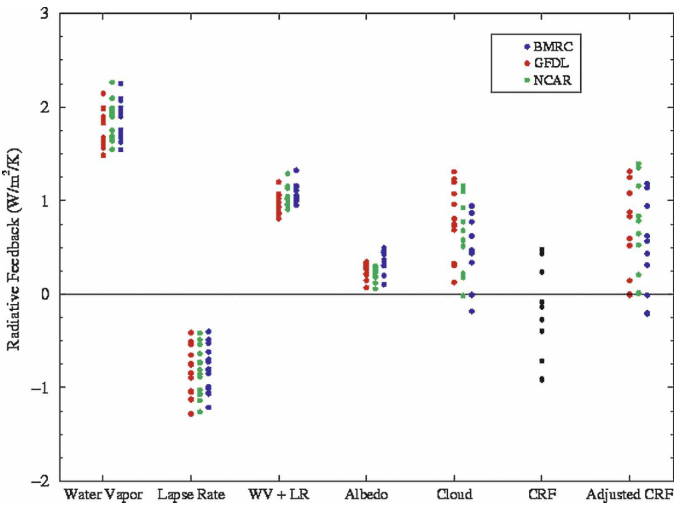
\includegraphics[width=.8\linewidth]{figs/polar_amp/fig7_Soden2008}
% 	\caption{The global-mean water vapor, lapse rate, water vapor$+$lapse rate, surface albedo, and cloud feedbacks computed for 14 coupled ocean–atmosphere models (listed in Table 1 of \cite{Soden2006}) using the GFDL (red), NCAR (green), CAWCR (blue) kernels. Adapted from the Figure 7 of \cite{Soden2008}.}
% 	\label{fig:soden2008_3_kernels}
% \end{figure}
%What's more, the radiative kernel can satisfy the goal to estimate the linearity of different climate feedbacks as the use of small differential changes is close to the "tangent linear" approximation that is the formal basis for the Taylor series expansion in Eq. (1) \citep{Feldl2013a}. 

To get the radiative kernels for one model, the model should produce high-frequency (typically either every time step or every 3 hours) output in order to get the instantaneous fields for the various variables that are needed. Initially, the model run is performed with profiles without perturbation in order to get the original TOA radiation fluxes, then run with profiles where a certain variable is perturbed at each level and each time step (e.g. 3 hours) to obtain the new TOA radiation fluxes corresponding to that perturbation. Specifically, the small perturbations are applied to surface temperature (+1 K), atmospheric temperature (+1 K) and specific humidity (the change amount is determined when temperature increases by 1 K but assuming relative humidity is constant) at each vertical level at each time step (e.g. 3 hours), respectively. In particular, the change of specific humidity $\Delta q$ for one layer is given by
\begin{equation}
\Delta q = q~\left(\frac{e_s(T+1)}{e_s(T)}-1\right),
\end{equation}
where $q, e_s$, and $T$ are specific humidity, saturation pressure of water vapor and temperature, respectively. $e_s$ satisfies Clausius–Clapeyron relation\index{Clausius–Clapeyron relation}, i.e. $\frac {\mathrm{d} e_s} {\mathrm{d} T} = \frac{L_v e_s}{R_v T^2}$,
where $L_v$ is the specific latent heat of evaporation of water, taken to as a constant value of $2.47\times 10^6$ J kg$^{-1}$ K$^{-1}$; $R_v$, with value of $461.5$ J kg$^{-1}$ K$^{-1}$, is the gas constant of water vapor. The simple method used in this study to estimate the saturated water vapor pressure is 
%The empirical equation \citep{Alduchov1996} is used to estimate $e_s$ (units: hPa) in this study:
%\begin{equation}
%e_ s ( T ) = 6.1094 \exp \left( \frac { 17.625 T } { T + 243.04 } \right),
%\end{equation}
\begin{equation}
e_s(T) = e_{s0}\exp\left[\frac{L_v}{R_v}\left(\frac{1}{T_0}-\frac{1}{T} \right)\right],
\end{equation}
where $e_{s0}$ is a reference value of $6.1078$ hPa for this at a reference temperature $T_0=273.16$ K. After each perturbation, the changes of radiation flux at TOA are recorded and then averaged over each month to get the kernels. In fact, the traditional kernels are supposed to compute under total-sky and clear-sky conditions separately so as to obtain the radiative effect of clouds, but only the clear-sky case will be calculated for the Isca model at present due to the lack of cloud schemes.

%\vspace{-0.3cm}
If $\Delta R$ represents the TOA radiation flux change due to the perturbation of variable $x$, then the radiative kernel for each level is defined as $K^i_x = \partial R / \partial x_i$, which is a function of space and time. In general, the resulting kernels are weighted relative to 100-hPa thick layer in order to make it easier to compare with other different kernels, that is $\mathbb{K}^i_x = K^i_x / \Delta p_i \times 100\text{ hPa}$, where $\Delta p_i$ is the thickness of layer $i$ in units of hPa. The total radiation flux change at TOA due to $x$ perturbation is obtained by integrating from the surface to the tropopause, that is
\begin{equation}
\Delta R=\sum_{i=1}^{nlev} \frac{\partial R}{\partial x_i}{\Delta x_i},
\label{eq:delta_R_sum}
\end{equation}
where $nlev$ denotes the number of vertical levels. The tropopause height is determined following the approach developed by \cite{Soden2006}, which defines the tropopause ($H$) at $100$ hPa at the equator and $300$ hPa at the poles and varies by cosine of latitude ($\phi$) in between, that is $H=300-200 \cos\phi$. After getting the radiation response, the climate feedback parameter is defined as

%\begin{equation}
%    \Delta R=\sum_{i=1}^{n} \frac{\partial R}{\partial x_i}{\Delta x_i},
%\end{equation}
%The cliamte feedback parameters are the product of the radiative kernel for relevant variable $x$ and the climate change anomaly normilized by the local surface temperature change
\begin{equation}
%\lambda = \frac{\Delta R}{\Delta T_s} = \sum_{i=1}^{n} \frac{\partial R}{\partial x_i}\frac{\Delta x_i}{\Delta 
\lambda = \frac{\Delta R}{\Delta T_s} = \frac{1}{\Delta T_s} \sum_{i=1}^{n} \frac{\partial R}{\partial x_i}\Delta x_i,
\label{eq:lambda_def}
\end{equation}
where $\Delta T_s$ is the surface temperature change and the units of $\lambda$ is Watt per meter squared per Kelvin (Wm$^{-2}$ K$^{-1}$).
% $\lambda$ can also be depicted in $K$ or $\mathbb{K}$, that is
%\begin{subequations}\label{eq:lambda_def_K}
%	\begin{equation}
%	%\lambda = \sum_{i=1}^{nlev} K^i \frac{\Delta x_i}{\Delta T_s},
%	\lambda =\frac{1}{\Delta T_s} \sum_{i=1}^{nlev} K^i \Delta x_i ,
%	\label{eq:lambda_def_K1}
%	\end{equation} 
%	\begin{equation}
%	% \lambda = \sum_{i=1}^{nlev} \frac{\Delta p_i}{100}\mathbb{K}^i  \frac{\Delta x_i}{\Delta T_s},
%	\lambda =\frac{1}{\Delta T_s}  \sum_{i=1}^{nlev} \frac{\Delta p_i}{100}\mathbb{K}^i  \Delta x_i,
%	\label{eq:lambda_def_K2}
%	\end{equation}
%\end{subequations}
%where $\Delta p_i$ is in units of hPa.
Note that zonal-mean variables, not the global-mean values, will be applied in \Eqref{eq:lambda_def} so we can analyze local or regional feedback, as it offers some advantages such as spatial pattern of changes \citep{Feldl2013,Feldl2017}.

In calculation of different climate feedbacks, different variables ($x$) will be employed in \Eqref{eq:lambda_def}. As for Planck feedback, the temperature change is vertically uniform in atmosphere, meaning that the air temperature change equals to the surface temperature change, so we have $x=T_s$ in \Eqref{eq:lambda_def}. Similarly, the lapse rate feedback is associated with the warming/cooling that deviates from surface temperature change, indicating that $x=T_a-T_s$ ($T_a$ denotes the atmospheric temperature) is utilized in \Eqref{eq:lambda_def}.
%Therefore, the Planck and lapse rate feedbacks can be rewritten as
% indicating that $\Delta x$ should be an array that have same size as atmospheric temperature but all the values are $\Delta T_s$.  , suggesting that $\Delta x$  has same size as atmospheric temperature but all of the values are $\Delta T_a-\Delta T_s$. 
%\begin{equation}
%\lambda_P = \frac{1}{\Delta T_s} \left( K_{T_s}\Delta T_s +\sum_i^{nlev} K_T^i \Delta T_s \right)%  = K_{T_s}+\sum_i^{nlev}K_T^i,
%\label{eq:fb_planck}
%\end{equation}
%and
%\begin{equation}
%\lambda_L =  \frac{1} {\Delta T_s} \sum_i^{nlev} K_T^i \left( \Delta T_{a}^i-\Delta T_s \right),
%\label{eq:fb_lapserate}
%\end{equation}
%respectively.
Regarding the water vapor feedbacks, the natural logarithm of atmospheric specific humidity (i.e. $x=\ln q$) is applied in \Eqref{eq:lambda_def}, since the absorption of radiation by water vapor is approximately proportional to the natural logarithm of water vapor content \citep{Shell2008,Feldl2016,Liu2018}. %However, we find that different equations are used to calculate water vapor feedback with kernel method. For example, \cite{Feldl2016} used the following equation to calculate the water vapor feedback:
%\begin{equation}
%\lambda_w = \sum_i^{nlev} K^i_q\frac{\Delta \ln q_i}{\delta \ln (q_{s}^i)}\frac{1}{\Delta T_s},
%\label{eq:wv_fb_feldl_eq}
%\end{equation}
%where $q_s$ is the saturated specific humidity. 
Similarly, \cite{Huang2017} employ another way to calculate the water vapor feedback:

\begin{equation}
% \lambda_w = \sum_i^{nlev} K^i_q ~\frac{\Delta \ln q_i}{(\delta e_s/ \delta T)_i} \frac{1}{\Delta T_s},
\lambda_w = \sum_i^{nlev} K^i_q ~\frac{\Delta \ln q_i}{(\delta \ln e_s/ \delta T)_i} \frac{1}{\Delta T_s},
\label{eq:fb_wv_YHuang}
\end{equation}
%and $(\delta e_s/ \delta T)_i$ is estimated by $\left(e_s(T_i+1)-e_s(T_i)\right)/ e_s(T_i)$, which is similar to the method that \cite{Pendergrass2018} used to calculate the water vapor kernel (refer to the scripts on \href{https://github.com/apendergrass/cam5-kernels}{https://github.com/apendergrass/cam5-kernels}), and hence we use \Eqref{eq:fb_wv_YHuang} to calculate the water vapor kernel in this study.
and $(\delta \ln e_s)_i$ is estimated by $\left(e_s(T_i+1)-e_s(T_i)\right)/ e_s(T_i)$, which is similar to the method that \cite{Pendergrass2018} used to calculate the water vapor kernel, and hence we use \Eqref{eq:fb_wv_YHuang} to calculate the water vapor kernel in this study.
%(refer to the scripts on https://github.com/apendergrass/cam5-kernels)

% ------------------- sub SECTION ------------------- %
\subsection{Radiative kernels in Isca}
 
To calculate the radiative kernels for Isca \index{Radiative kernel!of Isca|(}, a 10-year control experiment ($\alpha= 0.3$) is re-run for each radiation scheme to get the corresponding model outputs (e.g. temperature, specific humidity) at 3-hour frequency. Then 1-year climatology computed from the last 5-year period is taken as the basic profiles for the offline radiation codes. Then the perturbation procedure will be carried out for different variables such as surface temperature, atmospheric temperature and specific humidity to obtain the surface temperature, temperature and water vapor kernels respectively. The radiative kernel results for each radiation scheme are shown below and the data sets are available at Zenodo (\url{http://doi.org/10.5281/zenodo.4282681}).

\subsubsection{Frierson and BOG scheme}

\begin{figure}[ht]
	\centering
	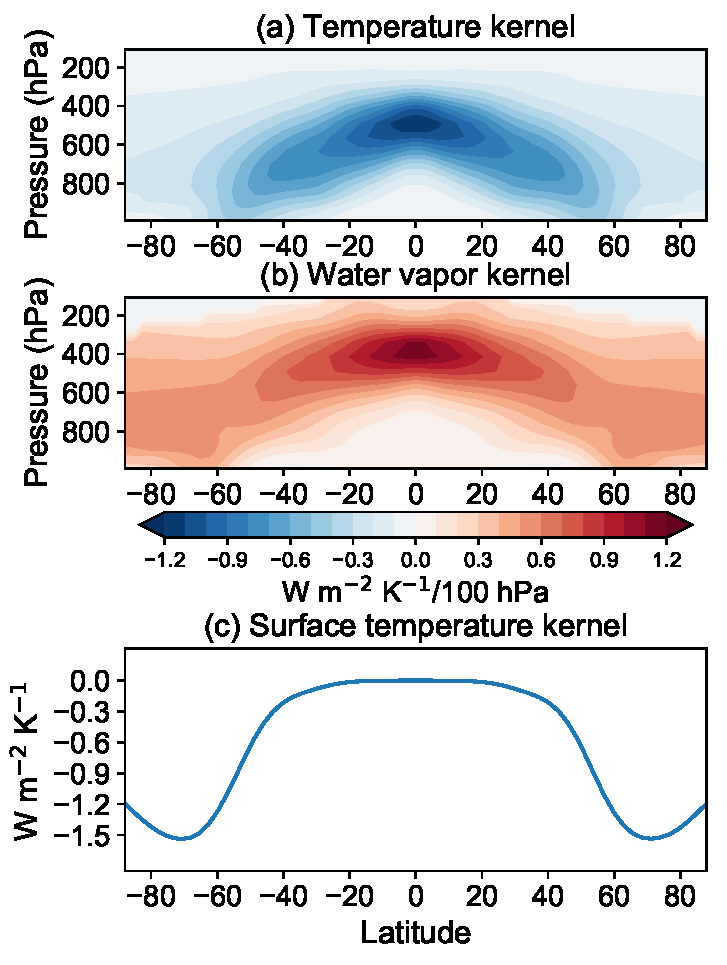
\includegraphics[width=0.45\linewidth]{figs/polar_amp/kernels_byrne}
	\caption[Annual-mean and zonal-mean temperature, water vapor and surface temperature radiative kernels for the BOG radiation scheme]{Annual-mean and zonal-mean radiative kernel for the Byrne and O'Gorman (BOG) radiation scheme: (a) temperature kernel with respect to 1-K increase in atmospheric temperature, (b) water vapor kernel for a specific humidity perturbation corresponding to a 1-K temperature increase with relative humidity unchanged, (c) surface temperature kernel for 1-K perturbation in surface temperature.}
	\label{fig:bog_kernels}
\end{figure}

% \begin{figure}[ht]
%   \begin{minipage}[c]{0.6\textwidth}
%     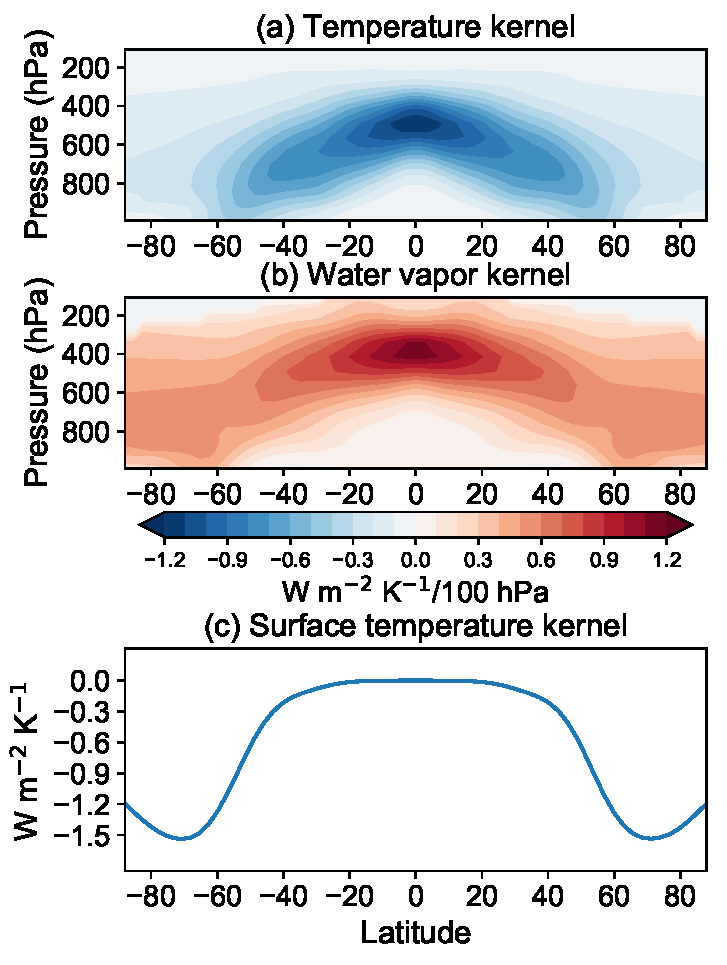
\includegraphics[width=\linewidth]{figs/polar_amp/kernels_byrne}
%   \end{minipage}
%   \hfill
%   \begin{minipage}[c]{0.35\textwidth}
%     \caption[Annual-mean and zonal-mean temperature, water vapor and surface temperature radiative kernels for the BOG radiation scheme]{Annual-mean and zonal-mean radiative kernel for the Byrne and O'Gorman (BOG) radiation scheme: (a) temperature kernel with respect to 1-K increase in atmospheric temperature, (b) water vapor kernel for a specific humidity perturbation corresponding to a 1-K temperature increase with relative humidity unchanged, (c) surface temperature kernel for 1-K perturbation in surface temperature.}
%     \label{fig:bog_kernels}
%   \end{minipage}
% \end{figure}

\begin{figure}[ht]
	\centering
	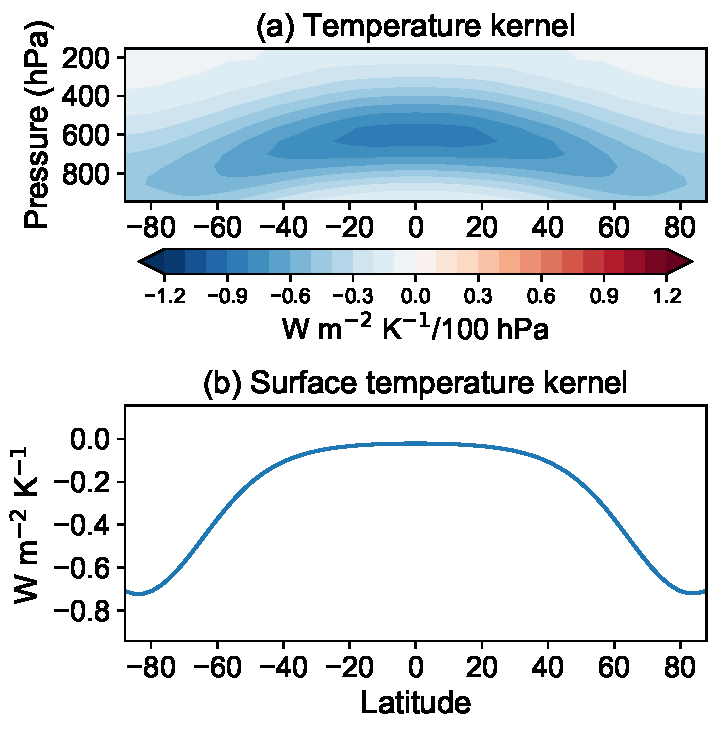
\includegraphics[width=0.45\linewidth]{figs/polar_amp/kernels_frierson}
	\caption[Annual-mean and zonal-mean temperature and surface temperature radiative kernels for Frierson radiation scheme]{As in \figref{fig:bog_kernels}, but only for temperature and surface temperature kernels in the Frierson radiation scheme.}
	\label{fig:frierson_kernels}
\end{figure}

%The shortwave radiation components for Frierson and BOG schemes are the same, where the insolation varies in diurnal cycle in the simulations. The only difference between these two gray radiation schemes lies in whether there is moisture feedback in longwave parts. Specifically, in the Frierson scheme, the optical thickness $\tau$ for longwave is defined as
%\begin{equation}
%\tau = \tau_{0}\left[f_{\text{l}}\left(\frac{p}{p_{\text{s}}}\right)+\left(1-f_{\text{l}}\right)\left(\frac{p}{p_{\text{s}}}\right)^{4}\right], \label{eq:frierson_optd}
%\end{equation}
%where $\tau_0$ is the optical depth at the surface, which is a function of latitude, $p_s$ and $p$ are pressure of surface and other vertical levels and $f_l$ is the coefficient to weight the linear and quartic terms, which is $0.1$ in the Isca. The quartic term approximates the structure of water vapor in atmosphere. The small linear term is included to reduce the stratospheric relaxation time. It is clear that the optical depth is specified in the Frierson scheme and won't change with the contents of water vapor in the model. However, the optical thickness in the BOG scheme vary with specific humidity $q$, as shown in the equation of $\tau$:
%\begin{equation}
%\frac{\text{d}\tau}{\text{d}\sigma}=a{\mu}+b{q}+c~\text{log}(CO_2/360),
%\label{eq:bog_optd}
%\end{equation}
%where $\sigma = p/p_0$, $\mu=1$ is a scaling parameter intended to represent absorption by well-mixed gases and $a$, $b$, $c$ are coefficients for different terms and the suggested values are $a = 0.1627, b = 1997.9$ and $c = 0.17$. 
%Shortwave parts introduce the zenith angles in the insolation...

The radiative kernels for temperature, water vapor and surface temperature in the BOG schemes are shown in \figref{fig:bog_kernels}. There is no water vapor kernel in the Frierson scheme (\figref{fig:frierson_kernels}). The temperature kernel illustrates the contribution of different latitudes and levels to the change of TOA longwave fluxes. The numerical values are generally negative, indicating that an increase in temperature increases the outgoing longwave radiation (negative feedback). As shown in \figref{fig:bog_kernels}a and \figref{fig:frierson_kernels}a, the values of temperature kernels are more negative in tropical atmosphere owing to the larger sensitivity according to the Stefan-Boltzmann law, but the location of largest sensitivity is somewhat different from the temperature kernel in the RRTM scheme (\figref{fig:rrtm_kernels}a), where the largest sensitivity appears near the surface in tropical regions. Low sensitivity occurs near the tropopause and polar region in the BOG's and Frierson's temperature kernel, reflecting the regional differences in lapse rate and emissivity \citep{Soden2008}. The vertically integrated global, annual mean of temperature kernel for the BOG and Frierson radiation schemes are -3.45 and -3.65 W m$^{-2}$ K$^{-1}$ respectively, which are similar to clear-sky temperature kernel for Geophysical Fluid Dynamics Laboratory (GFDL) atmospheric model (version AM2p12b), which is 3.6 W m$^{-2}$ K$^{-1}$ estimated by \cite{Soden2008}.

The water vapor kernel for the BOG scheme (\figref{fig:bog_kernels}b) demonstrates the relative importance of different level and latitudes to the strength of longwave water vapor feedback when temperature increases uniformly but the relative humidity keeps unchanged. In contrast, the values for water vapor feedback are positive almost everywhere, as the increase in the content of water vapor in atmosphere can help to increase the net incoming longwave radiation at TOA. Clearly, the water vapor kernel is largest in the deep tropics and decreases in the poleward direction. The vertically integrated global and annual mean for water vapor kernel in the BOG scheme is 3.61 W m$^{-2}$ K$^{-1}$, which is more than twice the clear-sky water vapor kernel (1.62 W m$^{-2}$ K$^{-1}$) of GFDL AM2p12b \citep{Soden2008}, suggesting that the water vapor feedback is much stronger in the BOG scheme.

The surface temperature kernel also contributes partially to the temperature feedback (the Planck feedback), and the warming of surface temperature increases the outgoing longwave radiation, so the surface temperature kernel is negative in all the latitudes as displayed in \figref{fig:bog_kernels}c and \figref{fig:frierson_kernels}b. But the scales of surface temperature kernel in the BOG and Frierson radiation schemes are different, and the possible reason for that is the surface temperature came from their own control runs rather than the same ones.

\begin{figure}[ht]
	\centering
	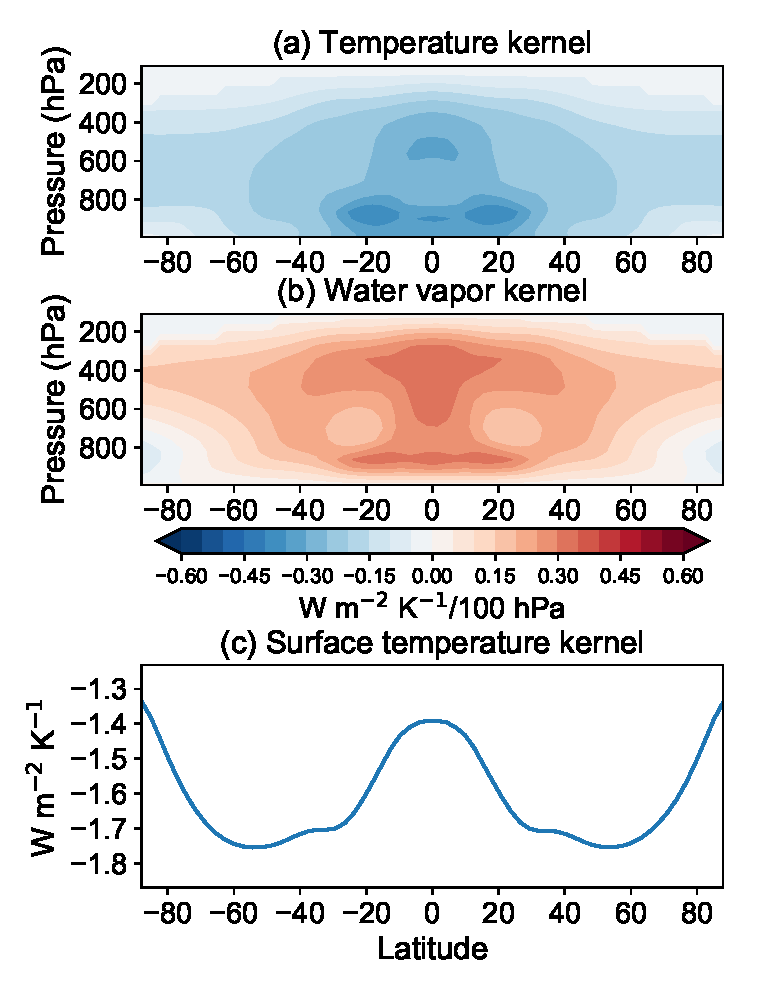
\includegraphics[width=0.45\linewidth]{figs/polar_amp/kernels_rrtm}
	\caption[Annual-mean and zonal-mean temperature, water vapor and surface temperature radiative kernels for the RRTM radiation scheme]{As in \figref{fig:bog_kernels}, but for the RRTM radiation scheme.}
	\label{fig:rrtm_kernels}
\end{figure}

\subsubsection{RRTM scheme} The offline version of RRTM code is from \textit{pyrrtm} (\url{https://github.com/tomflannaghan/pyrrtm}), which provides a user-friendly python wrapper for the single-column version of RRTM scheme. The input profiles for \textit{pyrrtm} are from the Isca outputs in which the albedo is 0.3. Nevertheless, one frustrating fact is that the single-column version of RRTM will consume too much time if we perturb each level and each position every 3 hours. In order to get over this drawback, we employ zonal-mean and monthly mean profiles as the input for the \textit{pyrrtm} to calculate the radiative kernels. As shown in \figref{fig:rrtm_kernels}a, the temperature kernel for the RRTM is weaker compared to the results of GFDL AM2.1 \citep[see their Fig. A1 of][]{Feldl2017coupled}, and the vertical integration of global and annual mean result is -1.79 W m$^{-2}$ K$^{-1}$, which is almost a half of the clear-sky results (-3.6 W m$^{-2}$ K$^{-1}$) of GFDL AM2p12b \citep{Soden2008}, suggesting that the feedbacks depending on this kernel would be small than other GCM's. However, the RRTM surface temperature kernel makes the situation different. It has a similar shape but the strength is much stronger compared to the surface temperature kernel of GFDL AM2.1 \citep[see their Fig. A1 of][]{Feldl2017coupled}, making the Planck feedback for the RRTM comparable (\figref{fig:all_feedbacks}c). With respect to the water vapor kernel for the RRTM, the vertical integration of global and annual mean value is 1.65 W m$^{-2}$ K$^{-1}$, which is close to the longwave water vapor kernel results (1.62 W m$^{-2}$ K$^{-1}$) of GFDL AM2p12b, meaning that the water vapor kernel is similar to other models. Although the positive values dominate the water vapor kernels, some negative values appear in the polar regions, as there are temperature inversions near the surface at high latitudes, which will decrease, rather than increase, the net longwave flux in response an increase of water vapor \citep{Soden2008}. However, this does not occur in water vapor kernel for the BOG radiation scheme (\figref{fig:bog_kernels}b).

% \begin{figure}[ht]
% 	\centering
% 	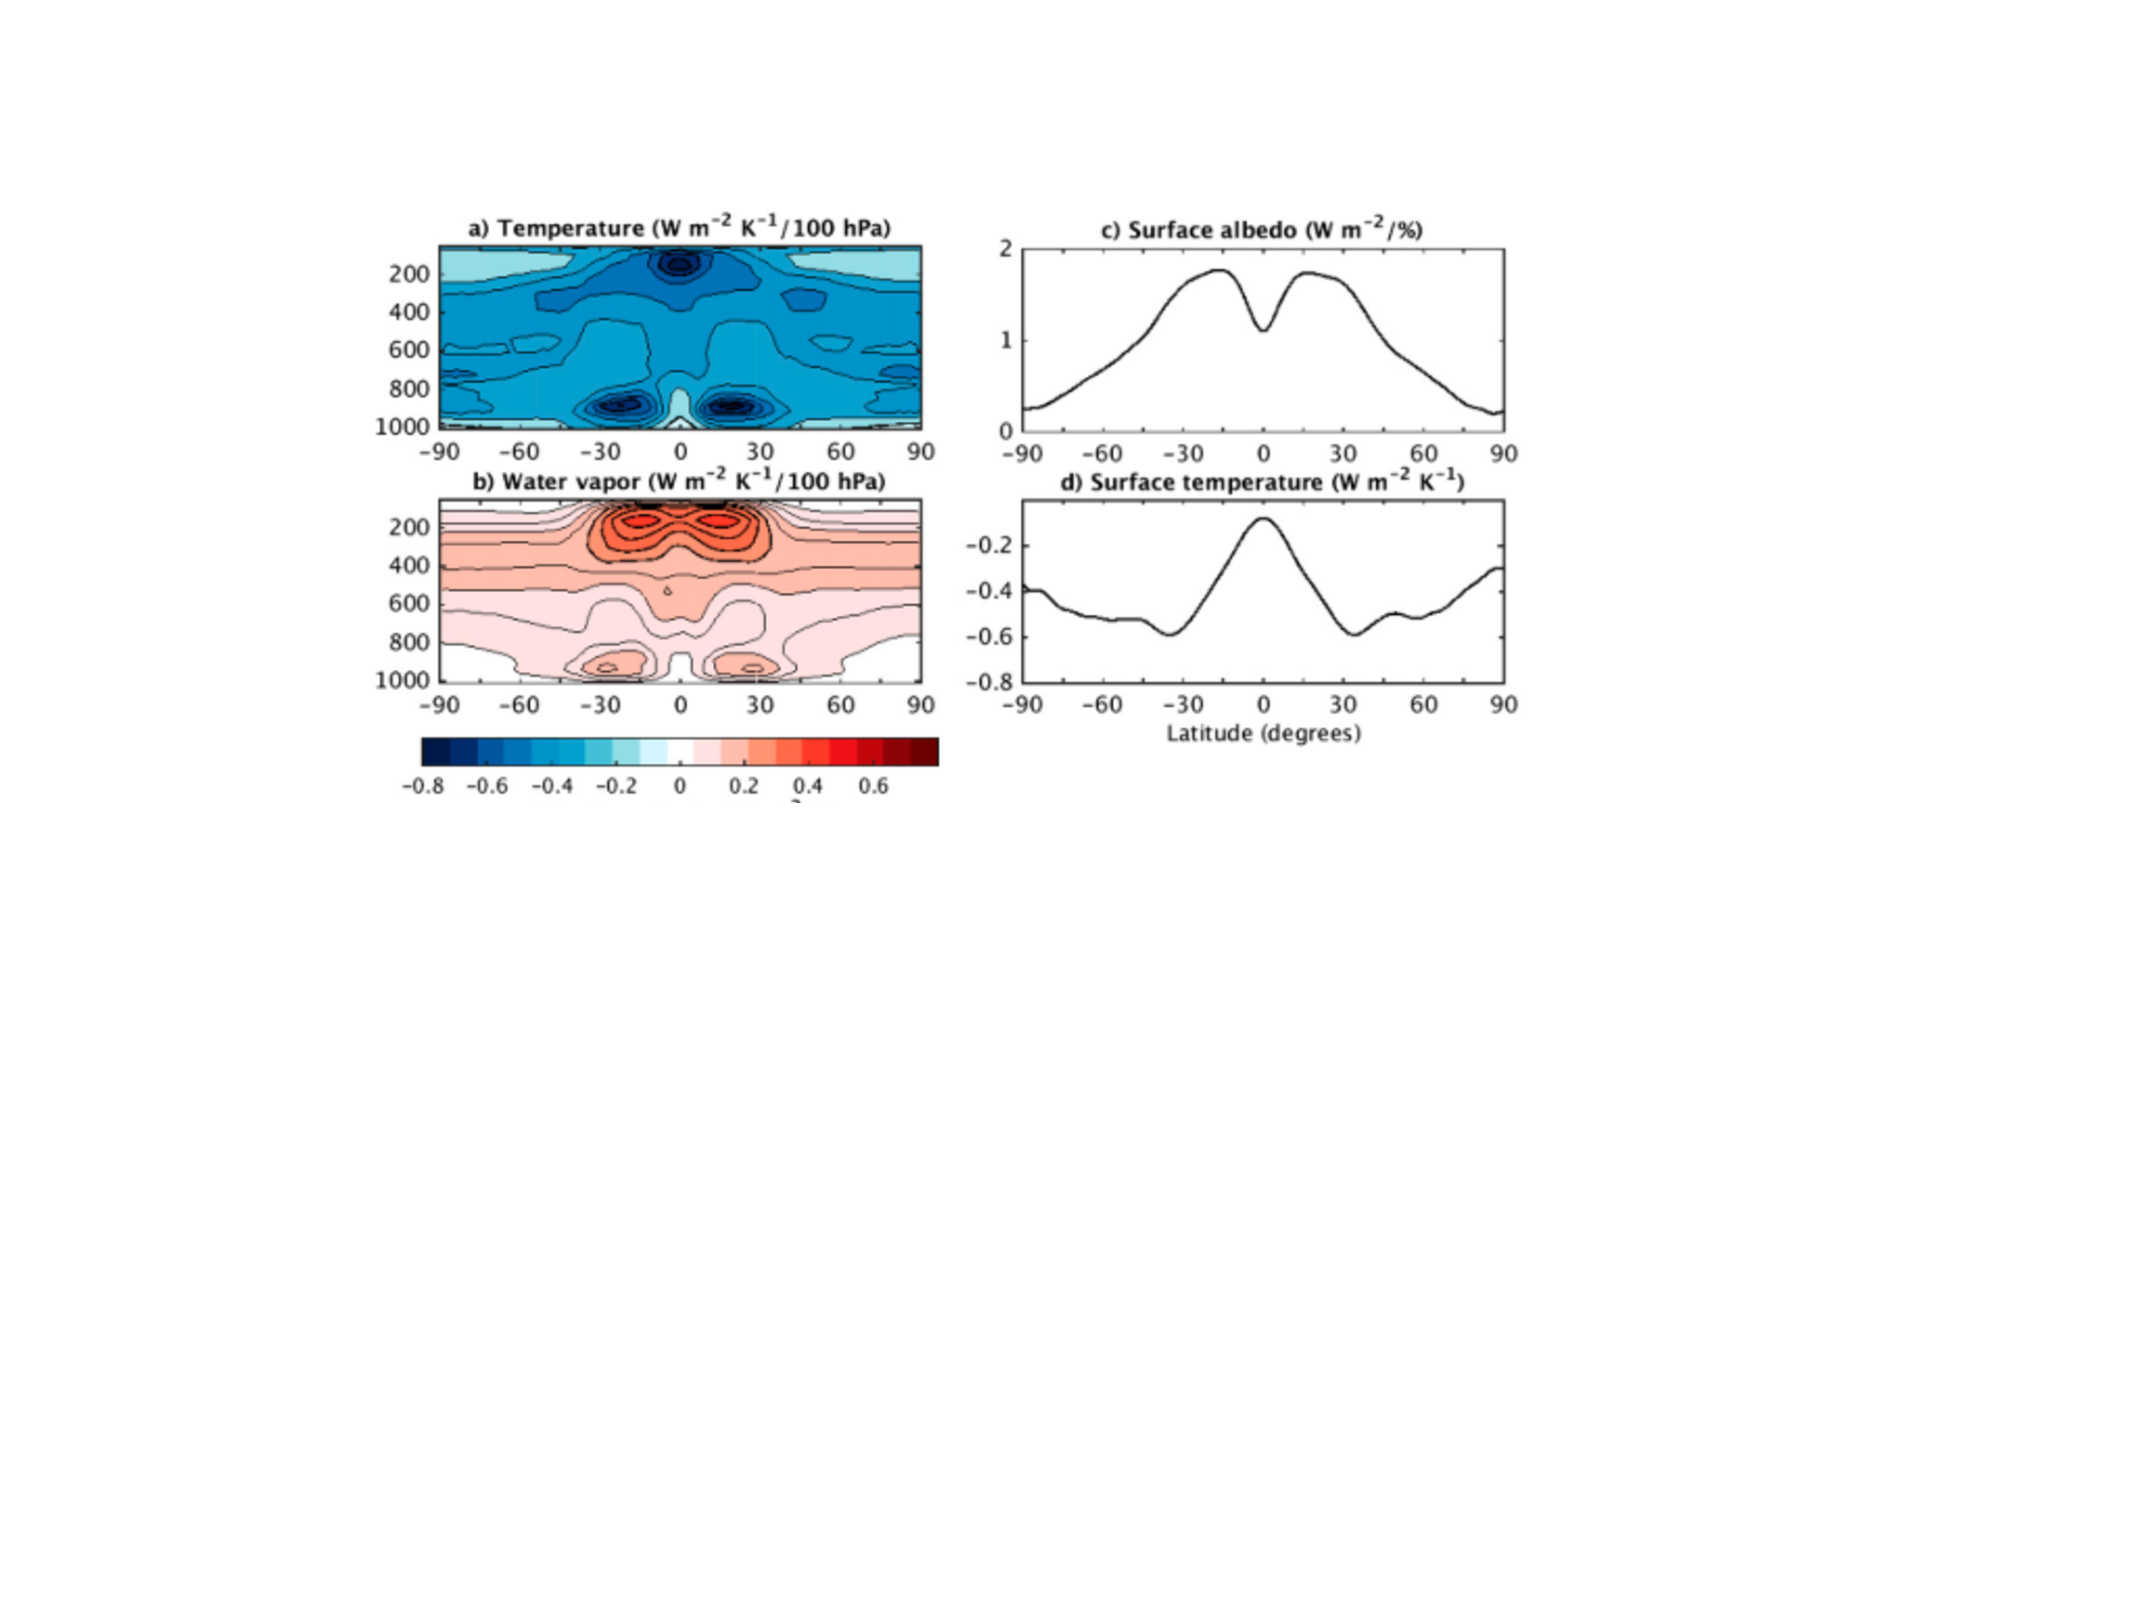
\includegraphics[width=.8\linewidth]{figs/polar_amp/Feldl2017}
% 	\caption[Annual-mean, zonal-mean radiative kernels for the GFDL AM2.1]{Annual-mean, zonal-mean radiative kernels for the GFDL AM2.1 aquaplanet based on a $4\times$ CO$_2$ simulation with daily mean solar zenith angle: (a) temperature kernel [W m$^{-2}$ K$^{-1}$ / 100 hPa], (b) water vapor kernel for a specific humidity perturbation corresponding to a 1-K temperature increase and fixed relative humidity, (c) surface albedo kernel, and (d) surface component of the temperature kernel. Adapted from Figure A1 of \cite{Feldl2017coupled}.}
% 	\label{fig:feldl_gfdl_am2.1_kernel}
% \end{figure}

\begin{figure}[ht]
	\centering
	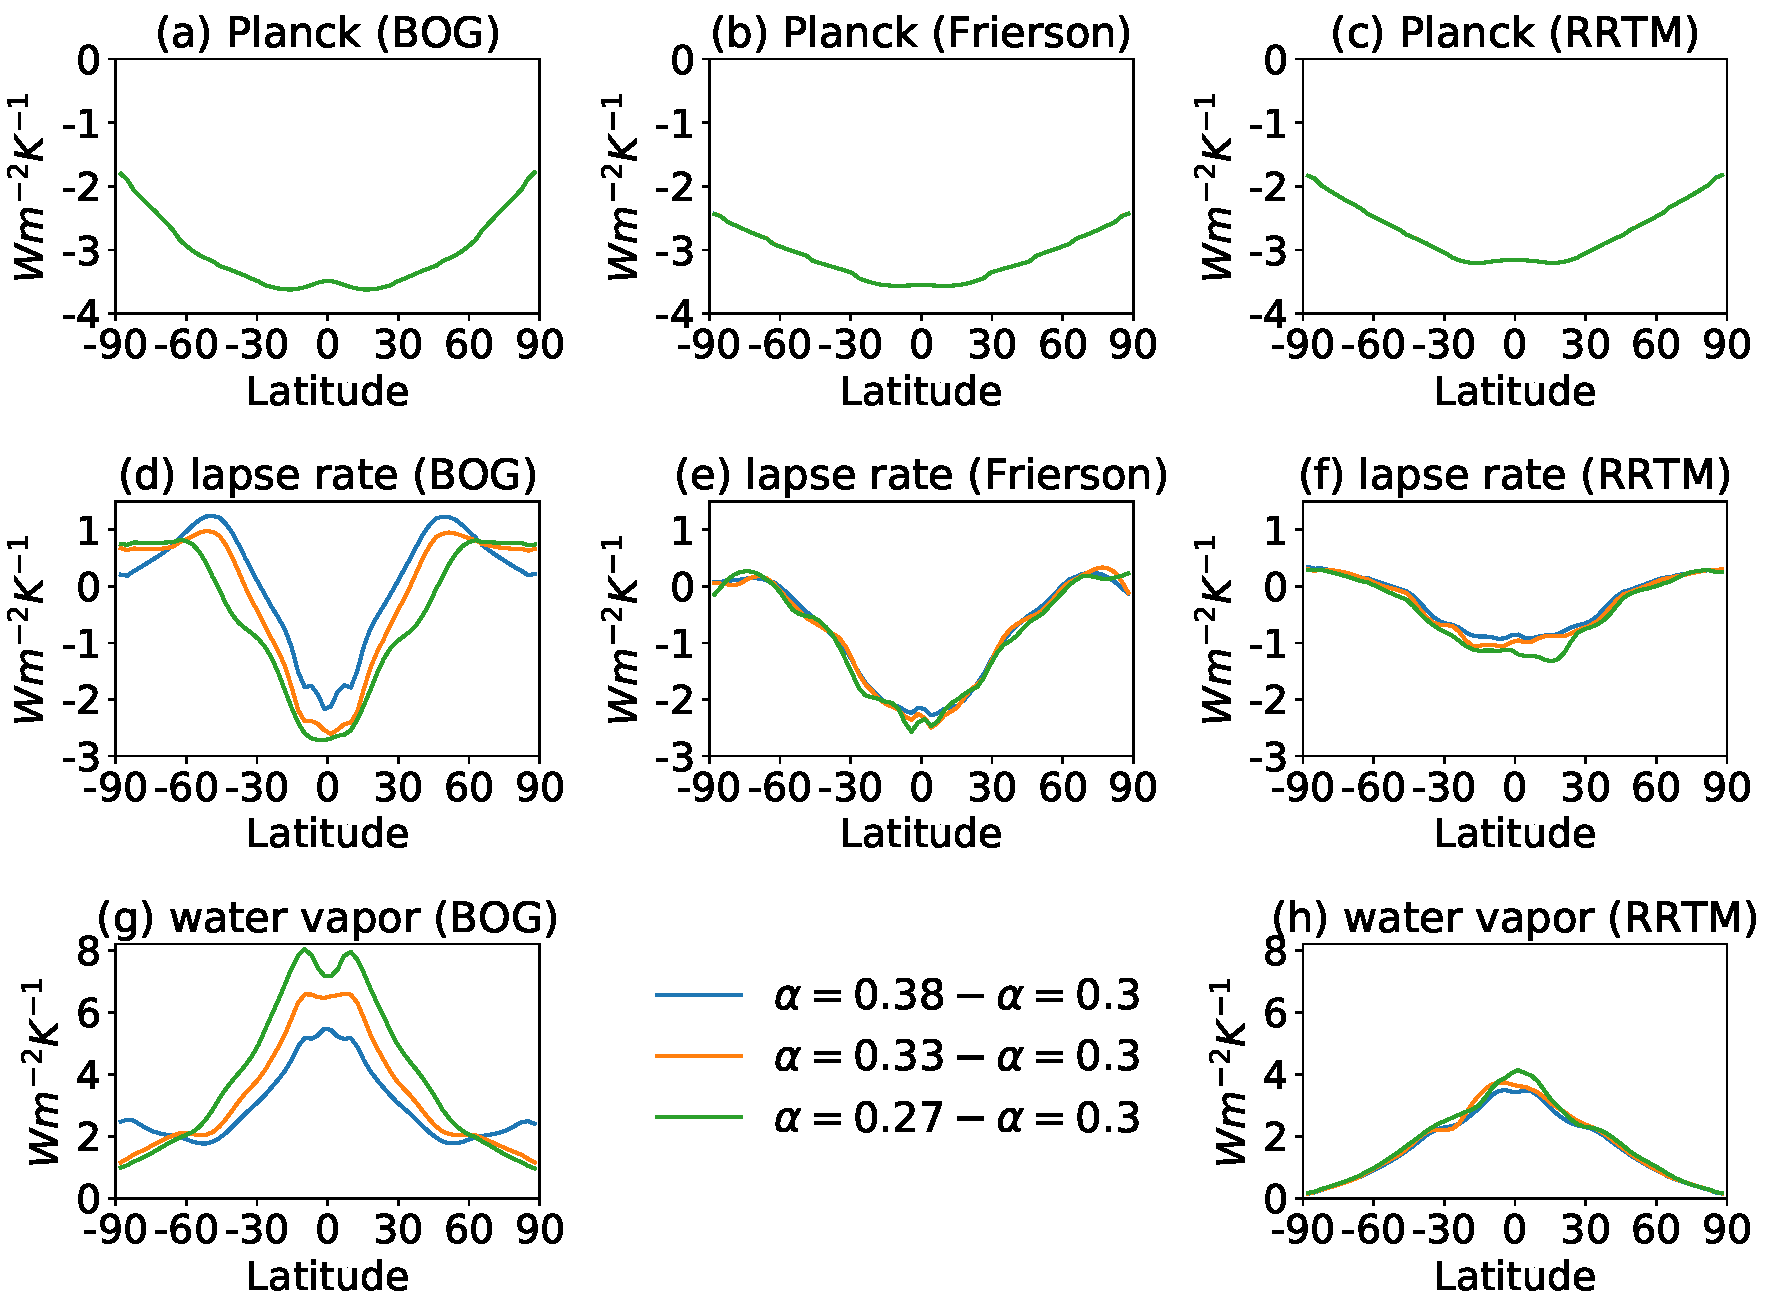
\includegraphics[width=0.8\textwidth]{figs/polar_amp/all_zonalmean_feedbacks}
	\caption[The zonal and annual mean climate feedback parameters for all the experiments in the BOG, Frierson and RRTM radiation schemes]{The zonal and annual mean climate feedback parameters for all the experiments in the BOG, Frierson and RRTM radiation schemes, where (a)-(c) are for the Planck feedbacks, (d)-(f) for the lapse rate feedbacks and (g)-(h) for the water vapor feedbacks. Blue, orange and green lines represent the experiments when albedo ($\alpha$) is changed from 0.3 to 0.38, 0.33 and 0.27 respectively.}
	\label{fig:all_feedbacks}
\end{figure}

\index{Radiative kernel!of Isca|)}

\subsection{Climate feedbacks in the Isca}
For each radiation scheme, the albedo parameter is changed from 0.3 to 0.27, 0.33 and 0.38 to provide an external forcing to the simulation respectively, leading to different degree of climate responses in the experiments. Thus in this section, we will use the radiative kernel technique to analyze the feedbacks for these experiments when changing albedos. The resulting Planck feedback, lapse rate feedback and water vapor feedback for each experiment are displayed in \figref{fig:all_feedbacks}.

% \begin{table}[ht]
% 	\centering
% 	\small
% 	\caption{Global mean lapse rate feedback parameters (Units: W m$^{-2}$ K$^{-1}$).}
% 	\vspace{0.5em}
% 	\label{tab:lapserate_fb}
% 	\begin{tabular}{cccc}
% 		\toprule
% 		Experiment & BOG & Frierson & RRTM \\
% 		\midrule
% 		$\alpha=$0.38 $-$ $\alpha=$0.3 & -0.33 & -1.23 & -0.51 \\
% 		$\alpha=$0.33 $-$ $\alpha=$0.3 & -0.84 & -1.28 & -0.61 \\
% 		$\alpha=$0.27 $-$ $\alpha=$0.3 & -1.15 & -1.32 & -0.72\\
% 		\bottomrule
% 	\end{tabular}
% \end{table}

% \begin{table}[ht]
% 	\centering
% 	\small
% 	\caption{Global mean water vapor feedback parameters (Units: W m$^{-2}$ K$^{-1}$).}
% 	\vspace{0.5em}
% 	\label{tab:wv_fb}
% 	\begin{tabular}{ccc}
% 		\toprule
% 		Experiment & BOG & RRTM \\
% 		\midrule
% 		$\alpha=$0.38 $-$ $\alpha=$0.3 & 3.38 & 2.14\\
% 		$\alpha=$0.33 $-$ $\alpha=$0.3 & 4.21 & 2.23 \\
% 		$\alpha=$0.27 $-$ $\alpha=$0.3 & 5.03 & 2.41\\
% 		\bottomrule
% 	\end{tabular}
% \end{table}

\begin{table}[ht]
	\centering
	\small
	\caption{Global mean lapse rate and water vapor feedback parameters (Units: W m$^{-2}$ K$^{-1}$).}
	\vspace{0.5em}
	\label{tab:lapserate_and_wv_fb}
	\begin{tabular}{cccccc}
		\toprule
		\multirow{2}{*}{Experiment} & \multicolumn{3}{c}{Lapse rate} & \multicolumn{2}{c}{Water vapor} \\
		\cline{2-4}\cline{5-6}
		{} & BOG & Frierson & RRTM & BOG & RRTM\\
		\midrule
		$\alpha=0.38 -\alpha=0.3$ & -0.33 & -1.23 & -0.51 & 3.38 & 2.14 \\
		$\alpha=0.33 - \alpha=0.3$ & -0.84 & -1.28 & -0.61 & 4.21 & 2.23 \\
		$\alpha=0.27-\alpha=0.3$ & -1.15 & -1.32 & -0.72 & 5.03 & 2.41 \\
		\bottomrule
	\end{tabular}
\end{table}

The Planck feedback \index{Feedback!Planck} is negative at all latitudes (\figsref{fig:all_feedbacks}a-c), meaning that an increase in temperature can increase the outgoing longwave radiation. In addition, the strength of the Planck feedback in the polar regions is weaker than the tropical region due to smaller blackbody emissions per unit warming at lower temperatures according to the Stefan-Boltzmann law \citep{Goosse2018}. The global mean Planck feedback parameters are -3.82, -3.79 and -3.41 W m$^{-2}$ K$^{-1}$ for the BOG, Frierson and RRTM radiation schemes respectively, showing that the differences of the Planck feedbacks in different radiation schemes are small. Regarding the lapse rate feedbacks, they are negative in low latitudes but positive in high latitudes, which is due to the different vertical distribution of temperature change in the polar regions compared to the tropics, as the temperature change is bottom heavy in the polar regions \citep{Pithan2014}. The global mean lapse rate feedback parameters for all experiments and all radiation schemes are listed in \tabref{tab:lapserate_and_wv_fb}. It is clear that the difference of global mean lapse rate feedbacks among different radiation schemes is large, but is small within the experiments with the same radiation schemes, except the one where the albedo is 0.38 in the BOG radiation scheme. As for water vapor feedback, it is positive in all experiments, implying that the net incoming longwave radiation increases in response to temperature warming. However, the spatial distribution of water vapor feedback is nonuniform, with high feedback in the tropics and small values in the polar regions (\figsref{fig:all_feedbacks}g and \ref{fig:all_feedbacks}h). This is because of the nonlinear effect of water vapor in response to warming. In addition, the global mean water vapor feedback parameters are displayed in \tabref{tab:lapserate_and_wv_fb}, where the water vapor feedback in the BOG schemes is almost twice of feedbacks in the RRTM scheme and the later is close to the water vapor feedback (2.01 W m$^{-2}$ K$^{-1}$) estimated by \cite{Soden2008} in GFDL AM2p12b, indicating that the water vapor feedback is much stronger in the BOG radiation scheme.

%%%%%%%%%%%%%%%%%%%%%% New section %%%%%%%%%%%%%%%%%%%%%%

\section{Results}
\label{sec:polar_amiplification_results}

%\subsection{Climate response}
\subsection{Surface temperature response}
\begin{figure}[ht]
	\centering
	%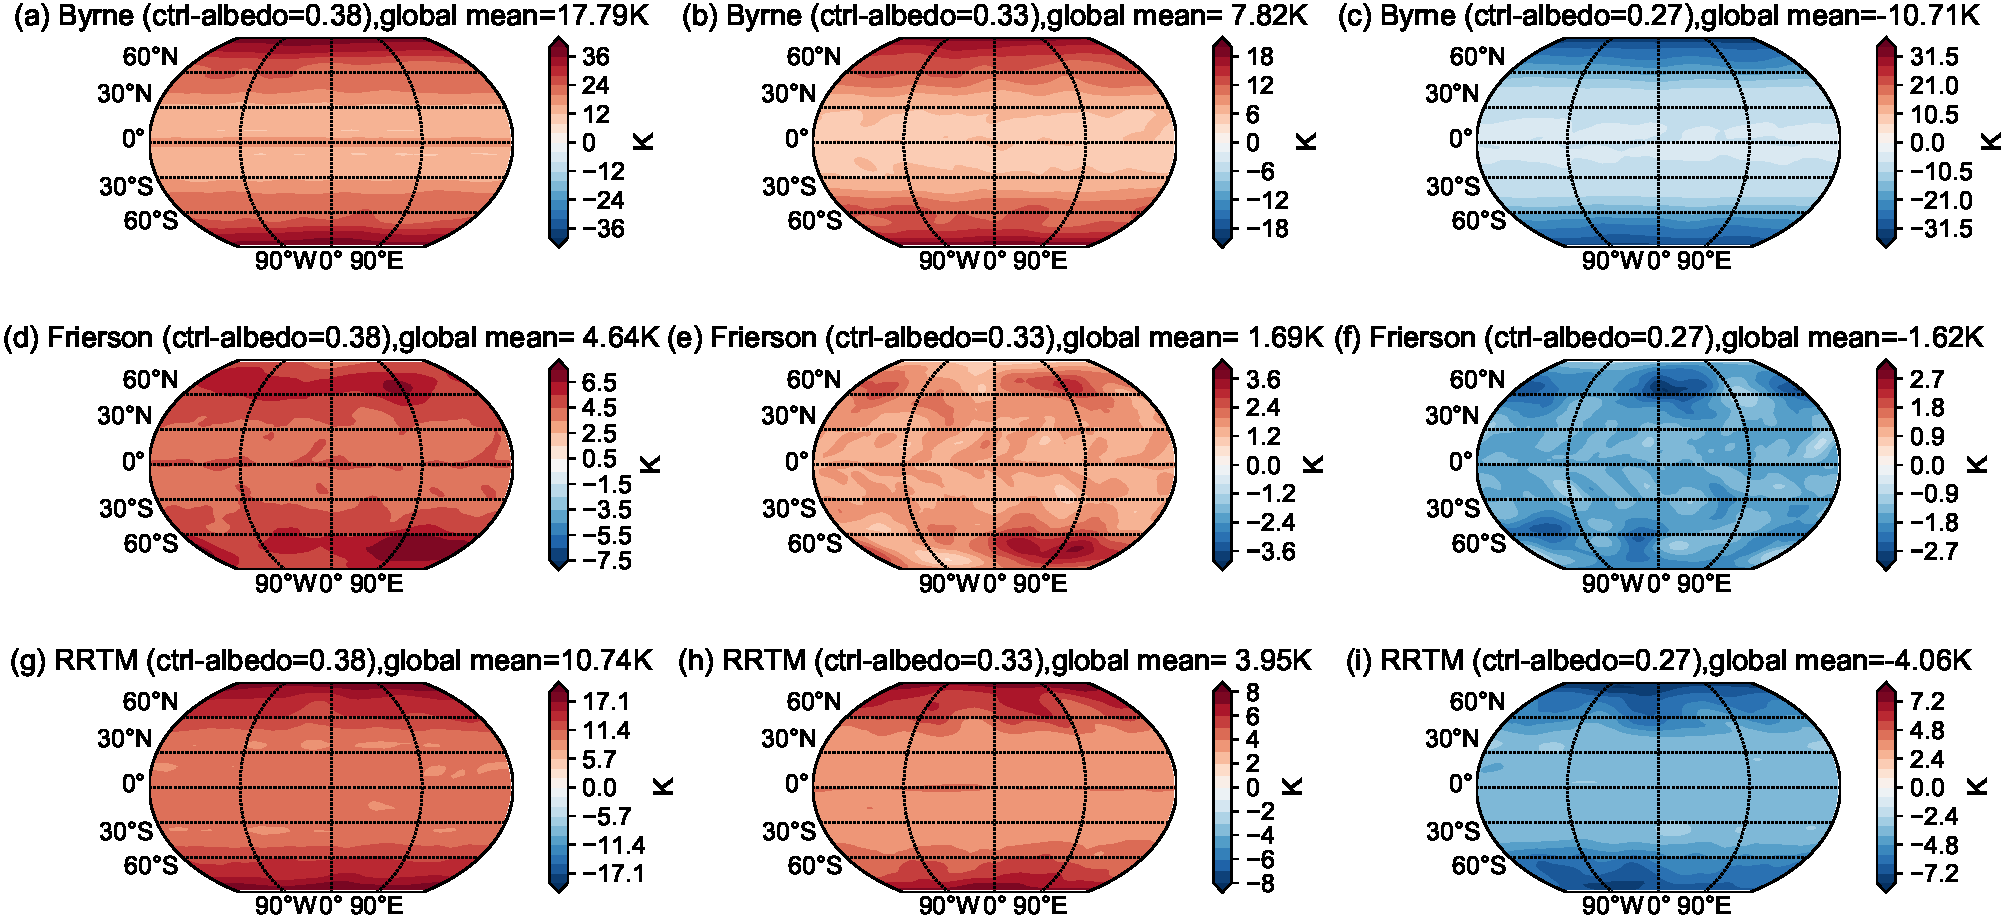
\includegraphics[width=1.0\linewidth]{{figs/polar_amp/tsurf_diff_ctrl_m_others_RdBu_kav7}.pdf}
	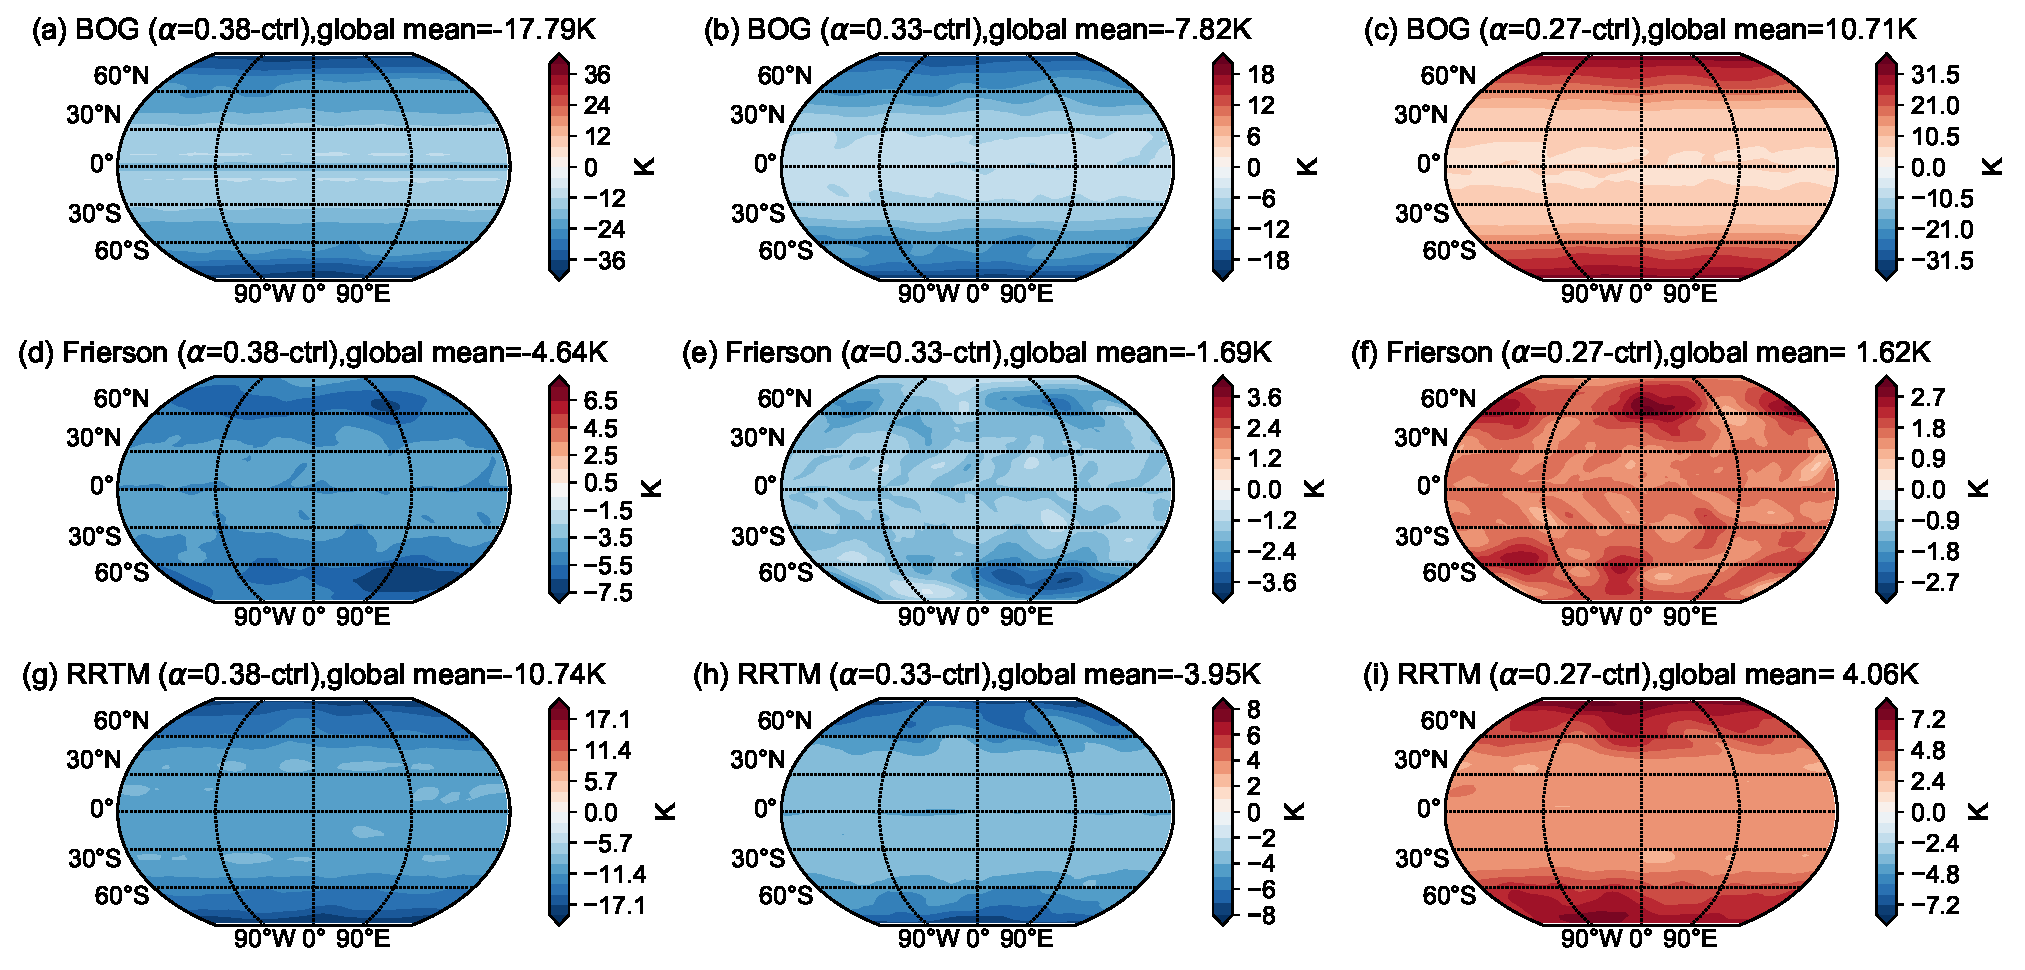
\includegraphics[width=1.0\linewidth]{{figs/polar_amp/tsurf_diff_others_m_ctrl_RdBu_kav7_2}.pdf}
	\caption[The spatial patterns of annual-mean surface temperature changes]{The global patterns of annual-mean surface temperature differences between the runs after changing albedos and the control run (i.e. $\alpha=0.3$) for the (a-c) BOG, (d-f) Frierson and (g-i) RRTM radiation schemes respectively, where the (a, d, g) left, (b, e, h) middle and (c, f, i) right panels represent the runs in which albedos are changed from 0.3 to 0.38, 0.33 and 0.27 respectively.}
	\label{fig:tsurf_diff}
\end{figure}

The global patterns of annual mean surface temperature differences after changing albedos for the BOG, Frierson and RRTM radiation schemes are displayed in \figref{fig:tsurf_diff}. The BOG scheme produces the largest surface temperate changes compared to the other two radiation schemes and Frierson scheme produces the weakest responses. For example, the annual and global mean surface temperature difference is 10.71K in the experiment where the albedo decreased 10\% from control run (i.e. from 0.3 to 0.27) for the BOG scheme. Global mean values are only 4.06K and 1.62K for the RRTM and Frierson schemes. Despite the fact that the responses are in relatively wide ranges, all simulation results from the three radiation schemes show polar amplified patterns either in the cooling or warming situations, which are clearly shown in the  annual and zonal mean patterns (\figsref{fig:delta_ts}a-c). The striking feature is that the strongest polar amplification pattern appears in the BOG scheme. However, the zonal mean surface temperature change in the Frierson scheme is almost flat with slight amplified cooling or warming at high latitudes but not exactly at the poles. Like the global mean surface temperature changes, the zonal mean patterns and the polar amplification are also moderate in the RRTM scheme among the three schemes.

To make the feature more evident, the zonal mean surface temperature responses are also normalized by the change in global mean surface temperature (\figsref{fig:delta_ts}d-f), showing that results from the Frierson scheme also have a slight polar amplification. Generally, the Arctic warming is almost twice as large as the global average in recent decades \citep{Serreze2006}. For example, the Arctic has a warming 1.9 times that of the globe on average in twelve IPCC AR4 models in CO$_2$ doubling experiments \citep{Winton2006surface}. As for the observed Arctic warming in the last half century, the zonal-mean Arctic warming is roughly 3 times greater than the tropical warming \citep{Merlis2018}. All results suggest that the ratios between polar and global temperature response seem a little surprising due to the lack of some feedback mechanisms such as surface albedo feedback in our experiments.

%% This weired behavior is due to the Q-flux, ocean heat transport...
% One strange thing in the BOG scheme is that annual and zonal mean surface temperature change in equator exhibits larger cooling relative to elsewhere in the tropics, for which the reasons will be investigated later. 
% 
%  and strongest polar amplification  showing various amplitudes in the surface temperature change

% Although the forcing changes by altering albedo differ from the way to double CO$_2$, the experiments illustrate that polar amplification can exist even in aquaplanet models.
% The zonal-mean and annual-mean surface temperature changes for each radiation scheme and albedo are presented in the,
%These results can also be quantified by the ratio between the surface temperature change in Arctic region and the globe or tropical region. 

%\begin{figure}[ht] %[ht]
%	\centering
%	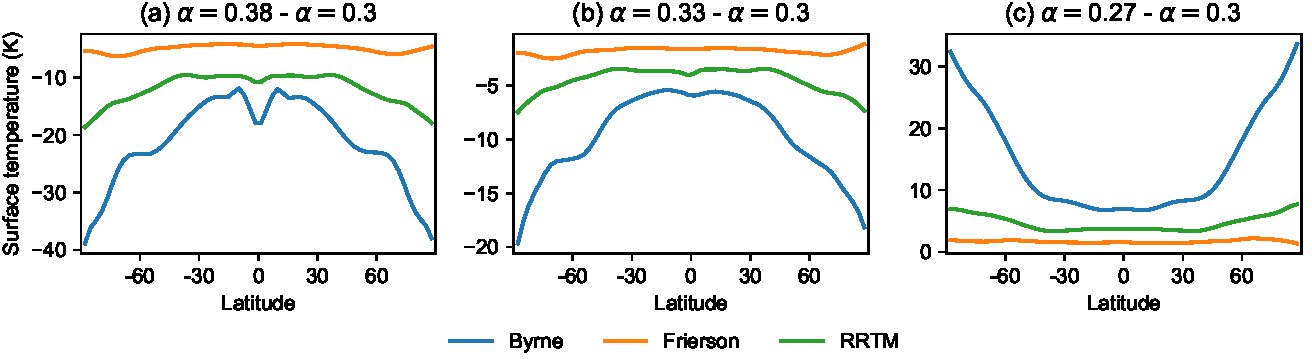
\includegraphics[width=1.0\linewidth]{{figs/polar_amp/tsurf_diff_zonal_mean_others_m_ctrl}.pdf}
%	\captionof{figure}{Temperatue difference when changing the global mean albedos (Annual and Zonal mean).}
%	\label{fig:tsuf_diff_zonal}
%\end{figure}

\begin{figure}[ht] % [ht]
	\centering
	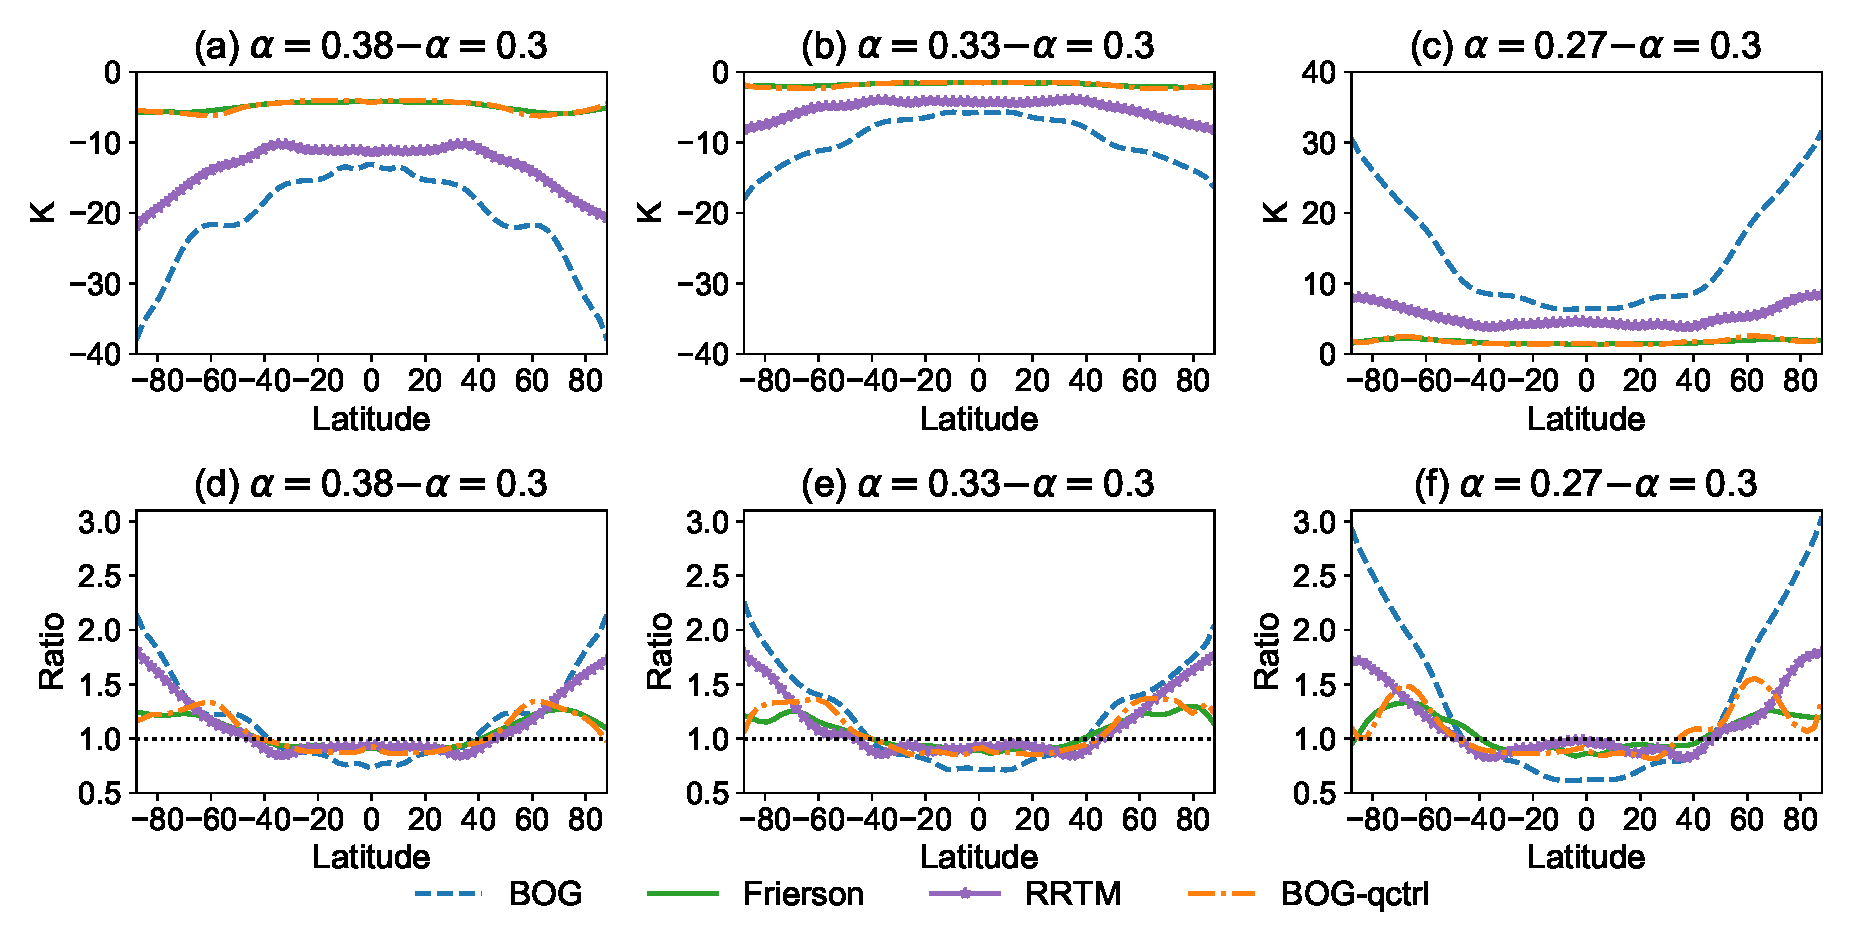
\includegraphics[width=1.0\linewidth]{figs/polar_amp/ts_diff.pdf}
	\caption[The zonal and annual mean surface temperature changes (top) and the change ratios with respect to global mean surface temperature change (bottom)]{The zonal mean and annual mean surface temperature changes for experiments where the albedo is changed from 0.3 to (a) 0.38, (b) 0.33 and (c) 0.3 respectively. Correspondingly, (d)-(f) show the ratios of surface temperature change at each latitude to the global mean surface temperature change for different simulations. Each experiment has been run in the BOG (blue dashed line), Frierson (green solid line) and RRTM (purple solid-starred line) radiation schemes respectively. The orange dash-dotted lines denote the experiments in the BOG scheme without moisture feedback.}
	\label{fig:delta_ts}
\end{figure}

\begin{figure}[ht] 
	\centering
	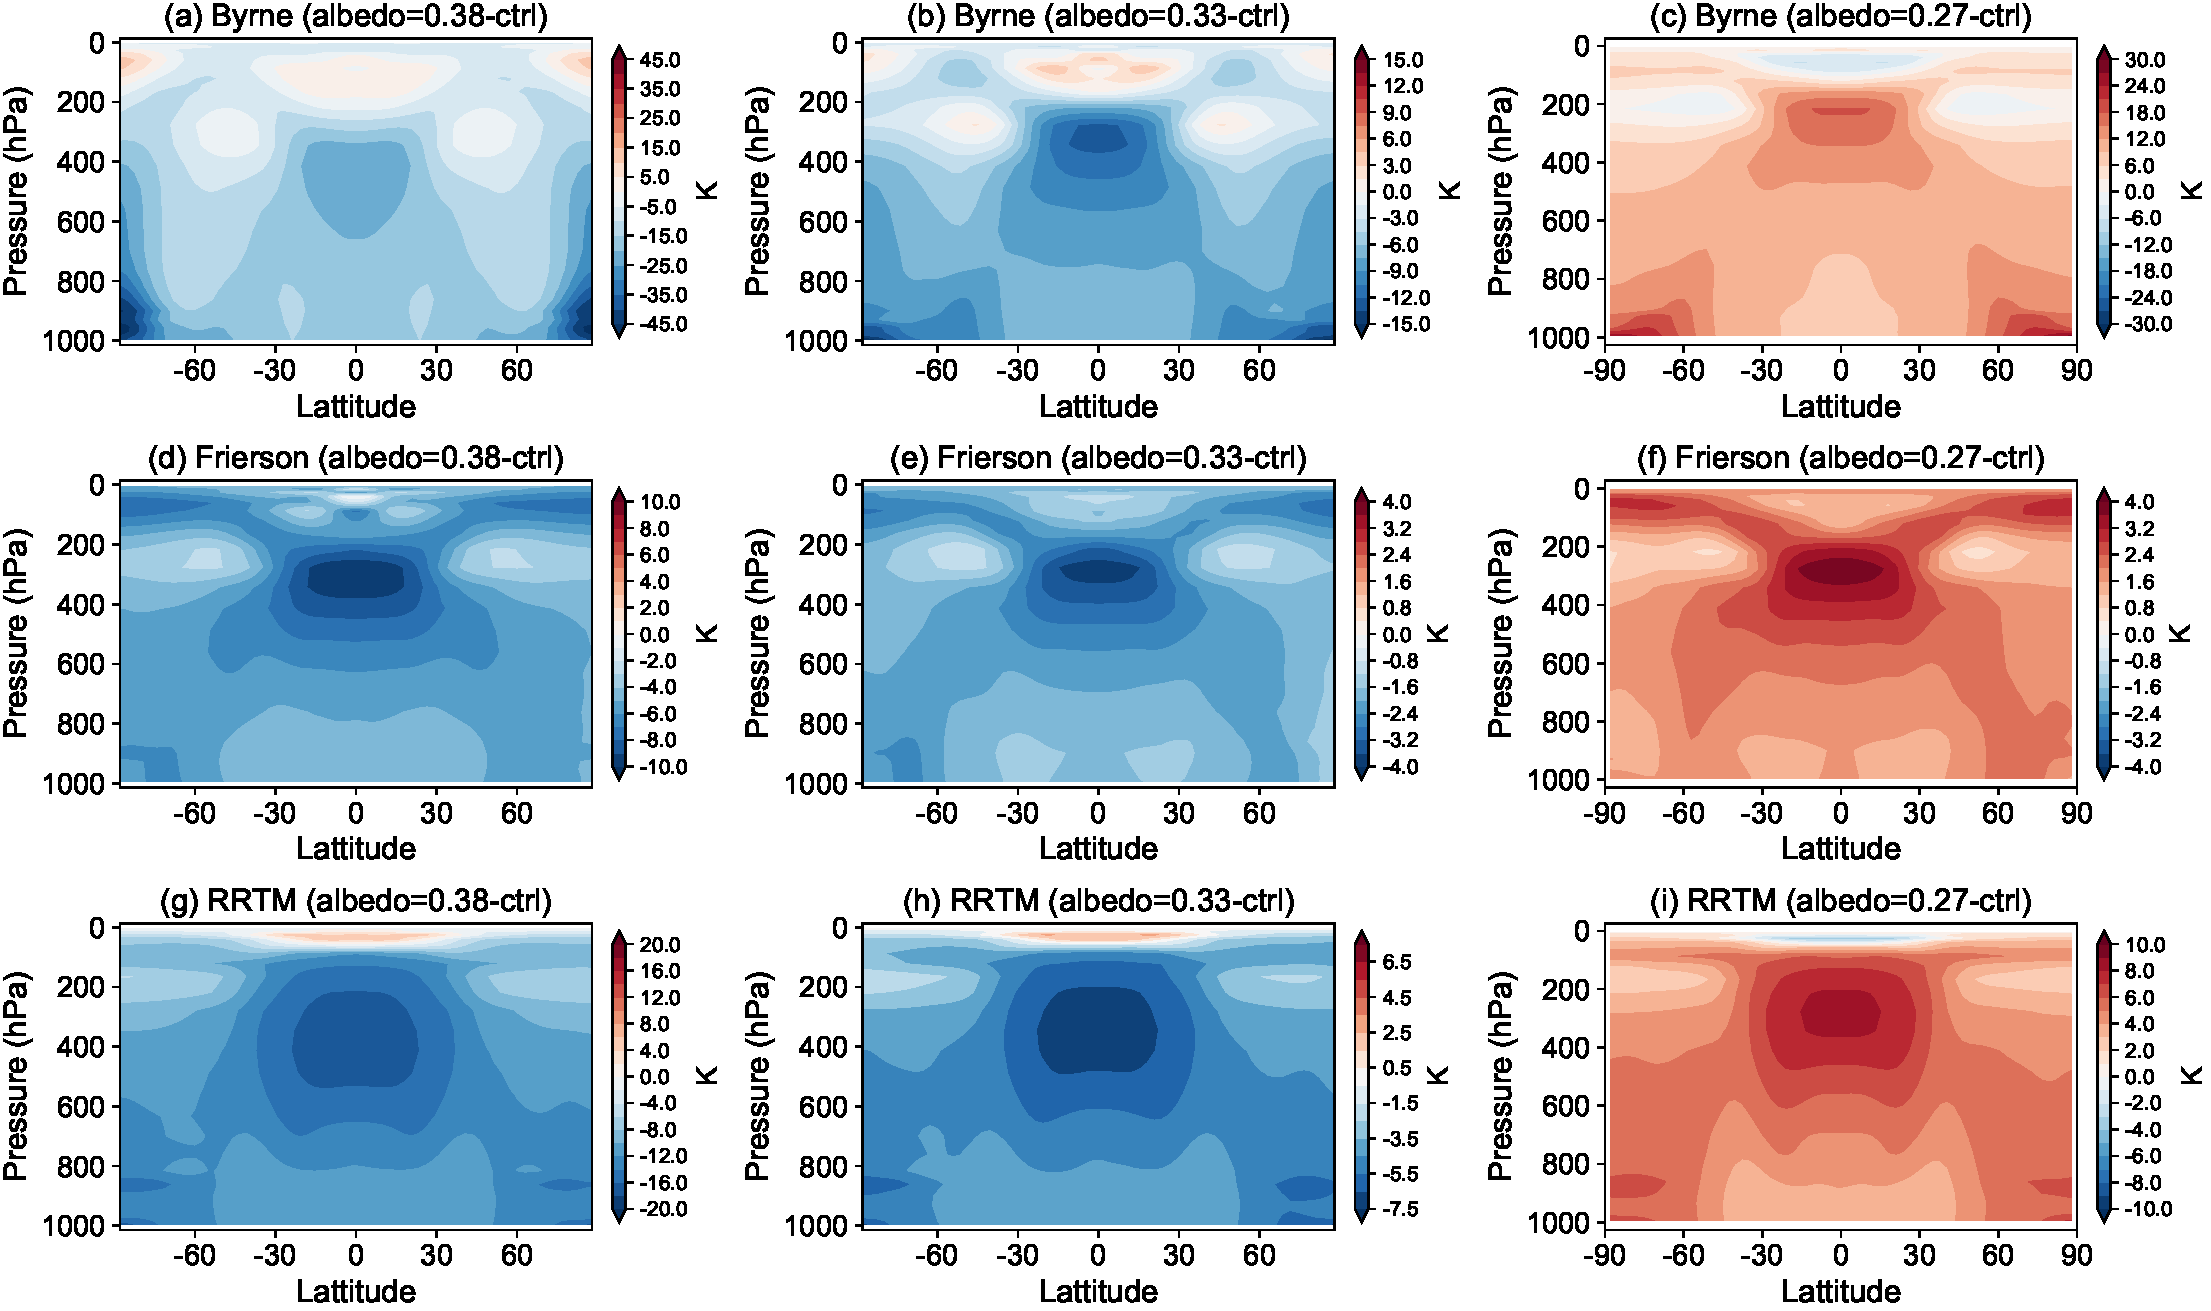
\includegraphics[width=1.0\linewidth]{{figs/polar_amp/temp_vert_profile_diff_others_m_ctrl_RdBu_symmetric}.pdf}
	\caption[The annual and zonal mean profiles of atmospheric temperature change]{The annual mean atmospheric temperature change profiles for experiments in (a)-(c) BOG, (d)-(f) Frierson and (g)-(i) RRTM radiation schemes. The (a, d, g) left, (b, e, h) middle and (c, f, i) right panels are for the experiments where albedos are altered from	 0.3 (control run) to 0.38, 0.33 and 0.27 respectively.}
	\label{fig:vert_temp_diff}
\end{figure}

%\caption{The annual and regional mean temperature differences in Arcitc and tropical regions and their warming (or cooling) ratio when changing the global mean albedos.}
% \begin{table}[ht]
	% \centering
	% \caption{The annual and regional mean temperature differences in  Arcitc and tropical regions and their warming (or cooling) ratio when changing the global mean % albedos.}
	% \begin{adjustbox}{width=1.0\textwidth,center=\textwidth}
	% \begin{tabular}{l c c c c c c c c c}
		% \toprule
		% \multirow{2}{*}{Region} & \multicolumn{3}{c}{Byrne(albedo=$x$-ctrl)} & \multicolumn{3}{c}{Frierson(albedo=$x$-ctrl)} & \multicolumn{3}{c}{RRTM(albedo=$x$-ctrl)}%  \\
		% \cline{2-4}  \cline{5-7} \cline{8-10}
		% & $x$=0.38 & $x$=0.33 & $x$=0.27 & $x$=0.38 & $x$=0.33 & $x$=0.27 & $x$=0.38 & $x$=0.33 & $x$=0.27\\
		% \midrule
		% Arctic & -30.53 & -14.47 & 26.70 & -5.52 & -1.87 & 1.94 & -15.13 & -5.99 & 6.36\\
		% Tropics & -14.64 & -5.69 & 6.86 & -4.35 & -1.58 & 1.52 & -10.12 & -3.72 & 3.71\\
		% Ratio & 2.09 & 2.54 & 3.89 & 1.27 & 1.19 & 1.27 & 1.50 & 1.61 & 1.72\\
		% \bottomrule
	% \end{tabular}
	% \end{adjustbox}
% \end{table}

To better understand the surface temperature responses, the structures of vertical atmospheric temperature changes are also investigated. As shown in \figref{fig:vert_temp_diff}, it is obvious that bottom-heavy cooling or warming profiles appear in the polar regions (\figsref{fig:delta_t_profile}a-c) in all the experiments, but top-heavy cooling or warming profiles appear in tropical upper troposphere (\figsref{fig:delta_t_profile}d-f). Many studies have found that this bottom-heavy structure is associated with polar amplification \citep{Screen2012, Pithan2014, Kim2018, Park2018}, as the stability in the polar region can trap more heat at the surface in the warming case, which hence leads to the positive lapse rate feedback in the polar region (\figsref{fig:all_feedbacks}d-f). In contrast, the lapse rate feedback is negative in the tropics, which means that in a warming climate, more latent heat will be released in the upper troposphere and thus cause greater warming in the upper troposphere than at the surface \citep{Pithan2014}.

It is worth noted that sea ice is responsible for the stable atmospheric structure in the polar region in the real world, but the stability of the polar region in our study is due to the equinox solar radiation. \cite{Kim2018} studied the sensitivity of polar amplification to insolation conditions and found that the equinox insolation brings larger static stability than seasonal or annual mean conditions due to the year-round near zero solar radiation reaching the polar region. Taking the warming case as an example, the active convection in the tropics induces a tight coupling between surface and upper troposphere, and a rising air parcel in warming climate will release more latent heat in the upper troposphere, decreasing the moist lapse rate \citep{Graversen2014}. Instead, the polar region is more stable and mixing with air aloft is harder than in the tropics, so that more heat is trapped near the surface, leaving a bottom heavy temperature structure and positive lapse rate feedback \citep{Pithan2014}. What is more, if we check closely the bottom heavy profile in the Frierson scheme, the largest warming or cooling near the surface occurs at about 70 degree not the poles (\figsref{fig:vert_temp_diff}d-f), which explains largest value of the zonal mean surface temperature change in the Frierson scheme in \figref{fig:delta_ts}.


In summary, polar amplification can exist in the aquaplanet model even without the sea ice and surface albedo feedback. Regarding the three radiation schemes we used in this study, the polar amplification of surface temperature is strongest in the BOG scheme, moderate in the RRTM and weakest in the Frierson scheme. As mentioned in \secref{sec:wv_fb_setup}, the crucial distinction between BOG and Frierson is whether there is moisture feedback in their longwave radiation schemes, which will be discussed further in \secref{sec:wv_feedback}. On the mechanisms about polar amplification, the bottom heavy structure of temperature difference provides some reasonable explanations for the polar amplification via lapse rate feedback, which will be investigated further in \secref{sec:climate_feedbacks_temp_decomp}.

\begin{figure}[ht]
	\centering
	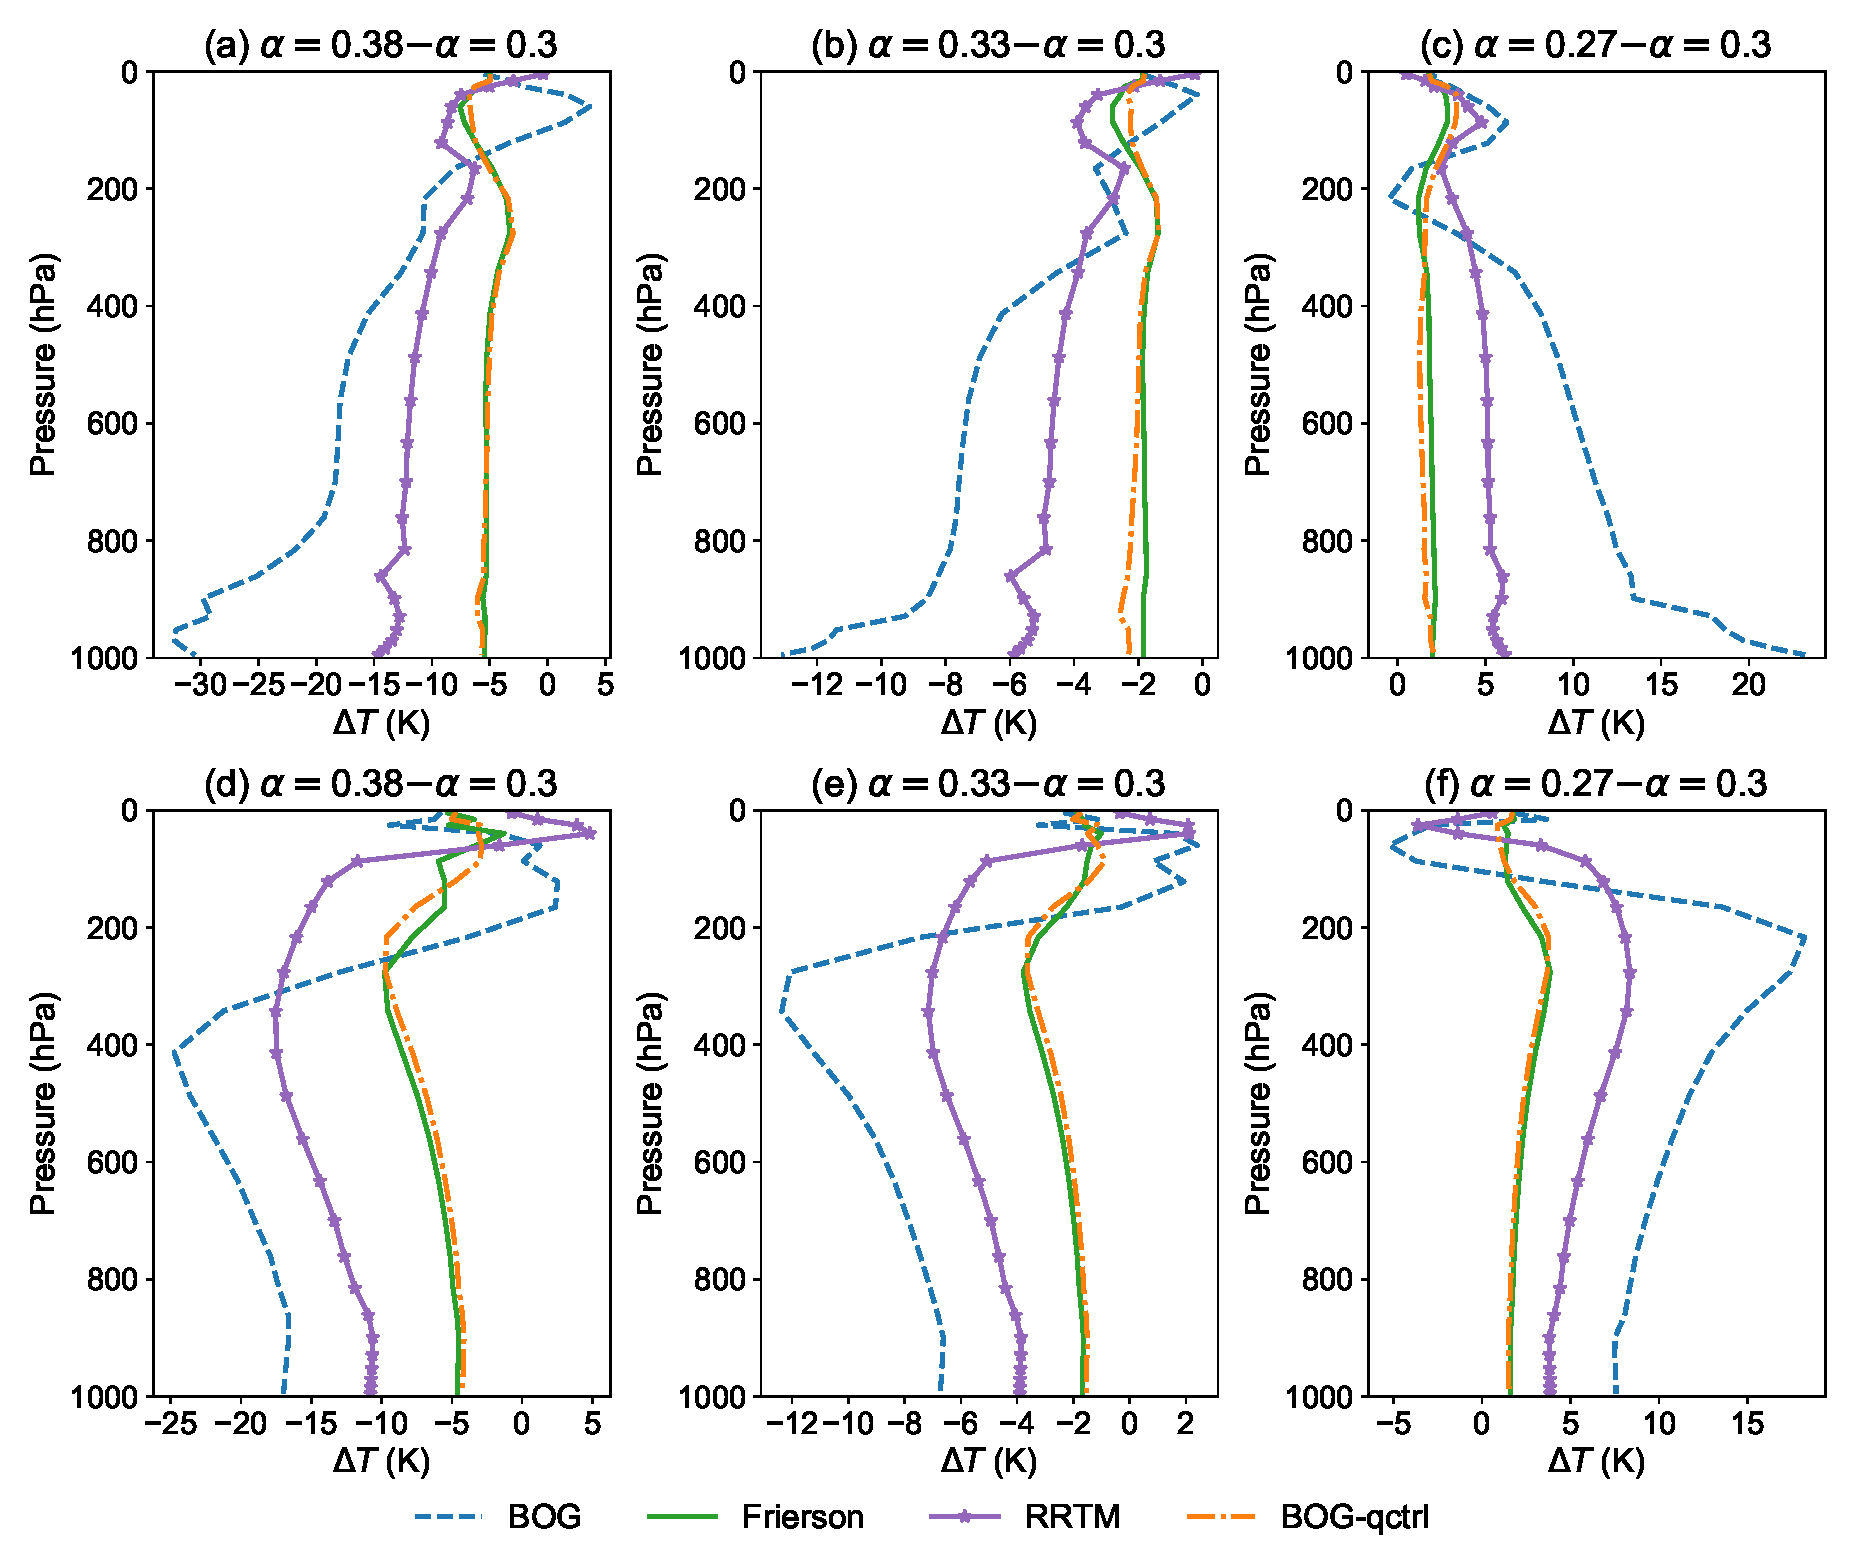
\includegraphics[width=0.8\linewidth]{figs/polar_amp/temp_profile}
	\caption[The annual mean profiles of atmospheric temperature change in polar (60$^\circ$N northward) and tropical (10$^\circ$S-10$^\circ$N) regions]{The annual mean profiles of atmospheric temperature change in (a-c) polar (60$^\circ$N northward) and (d-f) tropical (10$^\circ$S-10$^\circ$N) regions, where the left (a and d), middle (b and e) and right (c and f) panels are for the experiments where albedo is changed from 0.3 to 0.38, 0.33 and 0.27 respectively. The blue dashed, green solid and purple solid-starred lines denote BOG, Frierson and RRTM radiation schemes respectively. The orange dash-dotted lines denote the experiments in the BOG scheme without moisture feedback.}
	\label{fig:delta_t_profile}
\end{figure}


\subsection{Water vapor feedback}
\label{sec:wv_feedback}

\begin{figure}[ht]
	\centering
	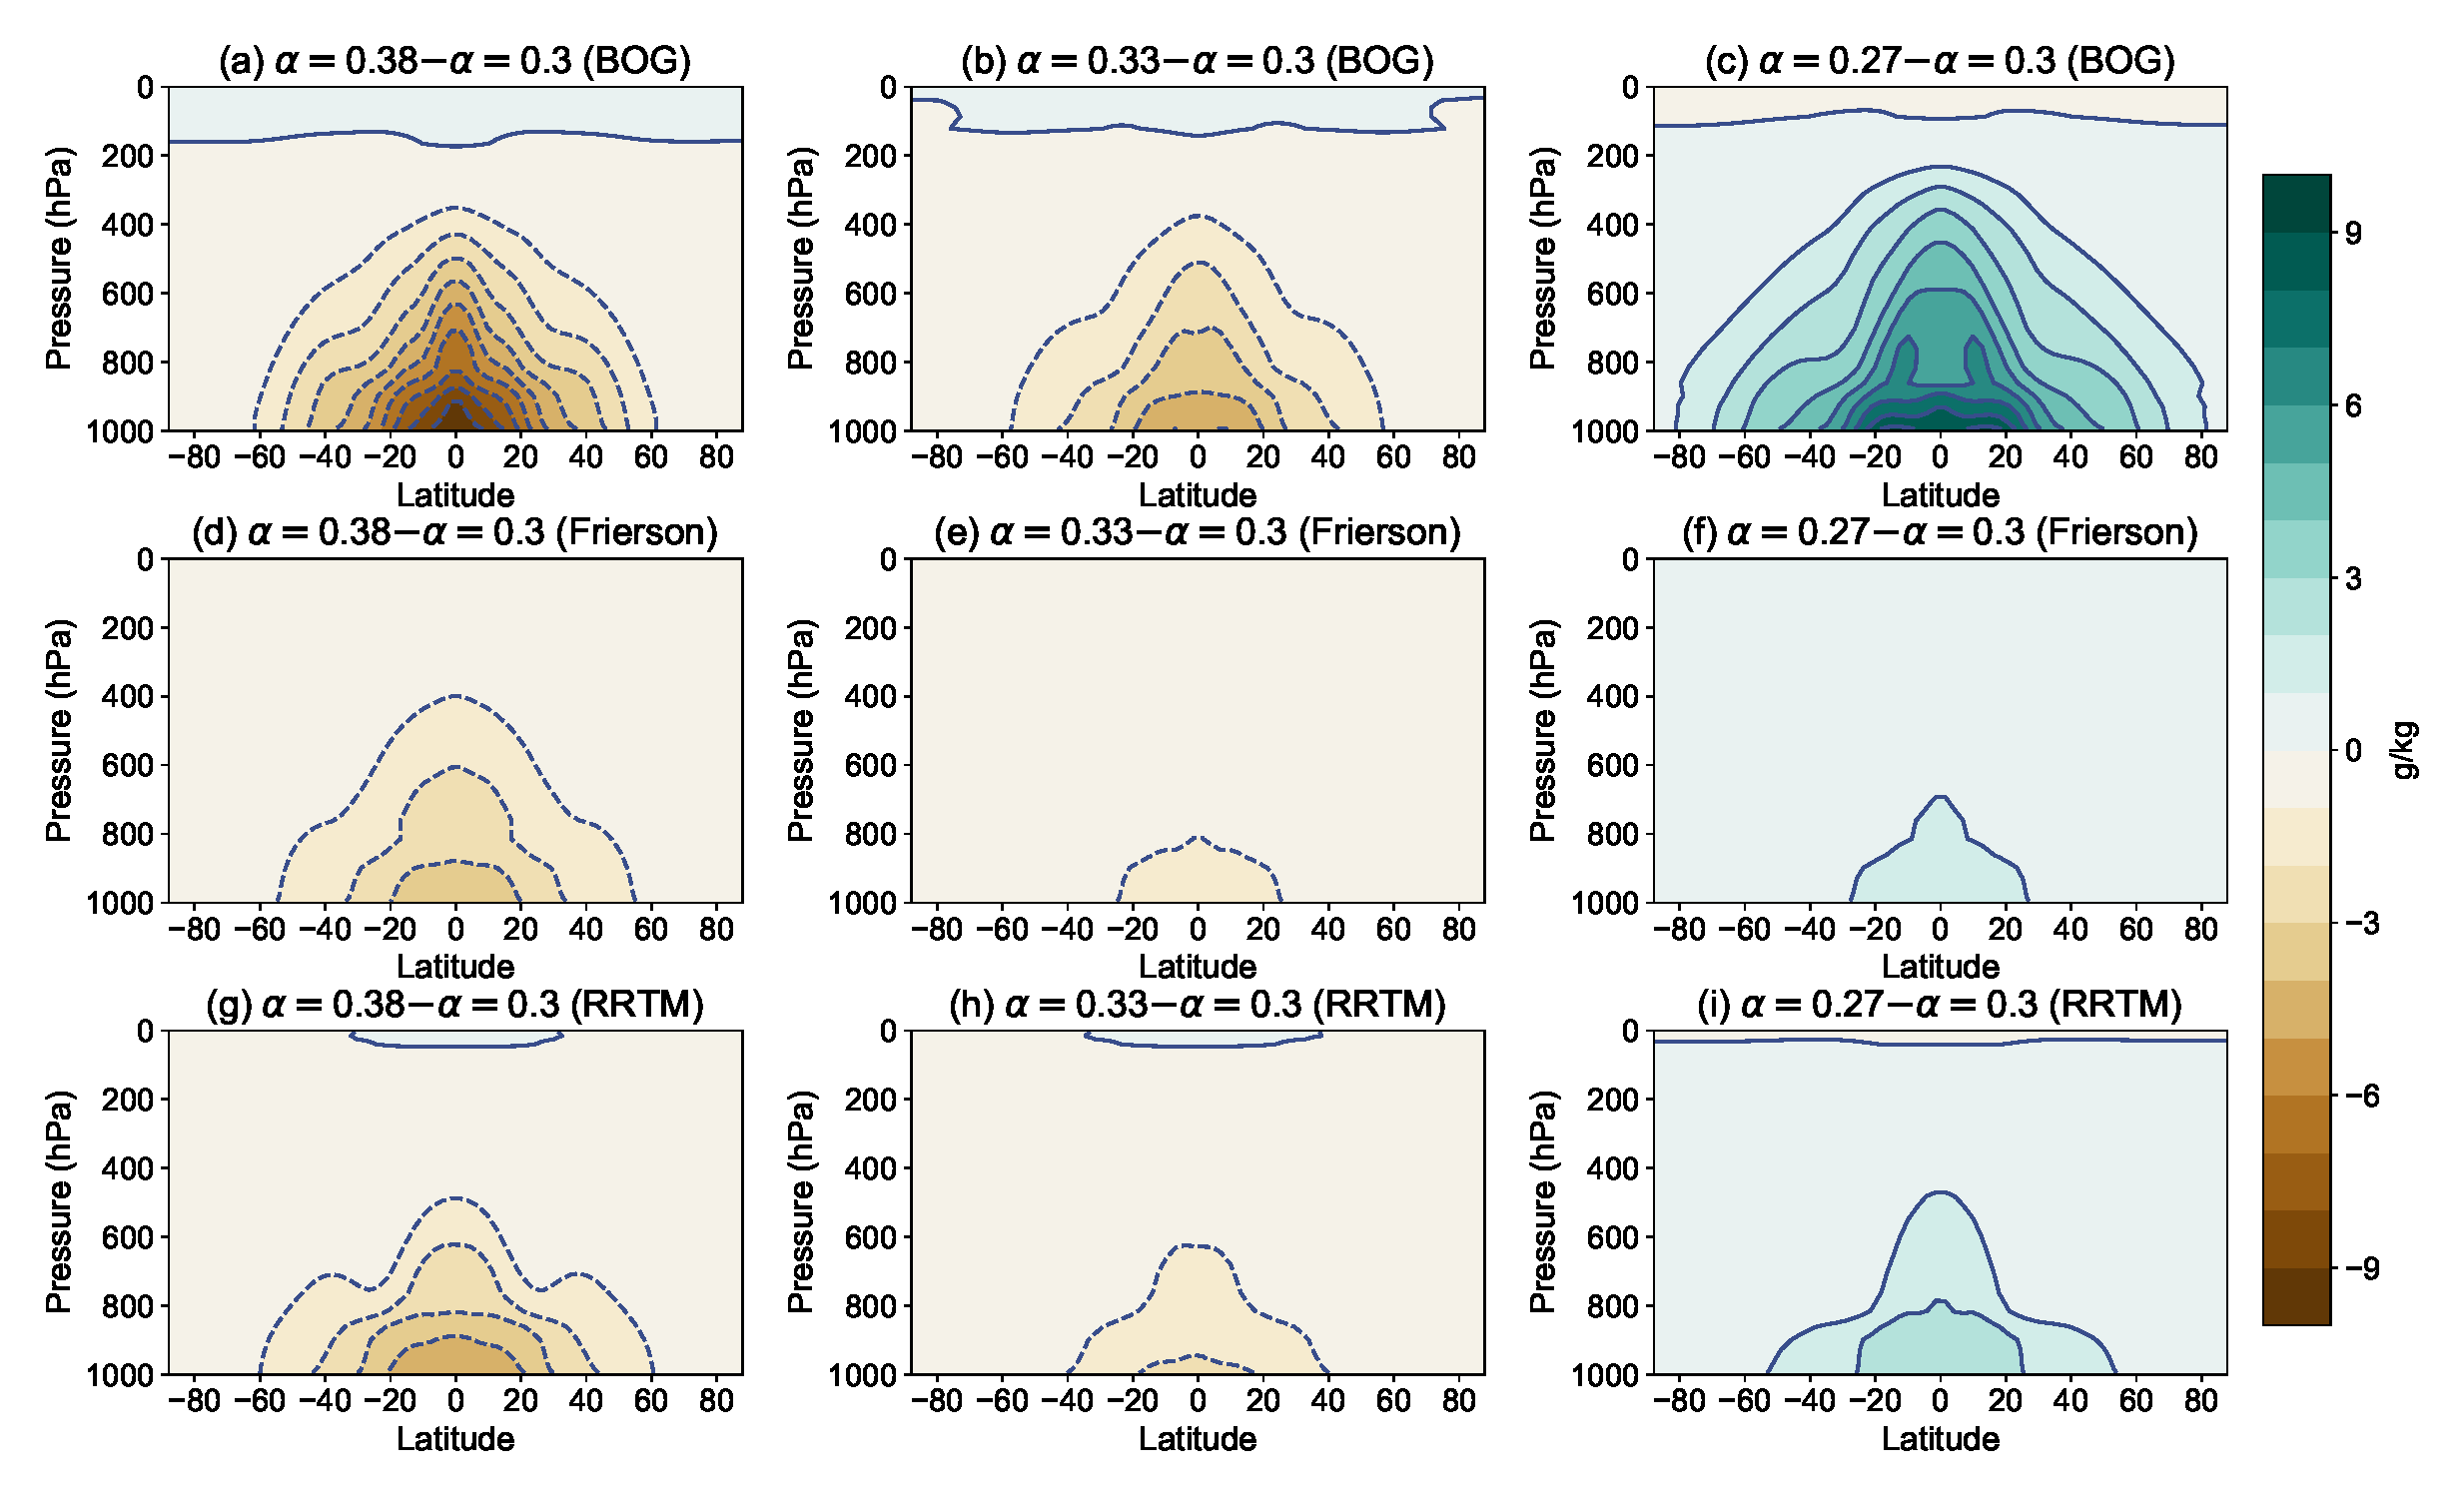
\includegraphics[width=1.0\linewidth]{figs/polar_amp/sphum_diff}
	\caption[The annual and zonal mean profiles of specific humidity changes]{As \figref{fig:vert_temp_diff}, but for the specific humidity change in the experiments with the BOG, Frierson and RRTM radiation schemes.}
	\label{fig:vert_q_diff}
\end{figure}

The annual and zonal mean changes in moisture profiles from different radiation schemes are shown in \figref{fig:vert_q_diff}. It is clear that the change of specific humidity profile is strongest in the BOG scheme and weakest in the Frierson scheme, both in the cooling and warming cases. Note that the specific humidity increases (decreases) in the warming (cooling) cases almost everywhere but most strongly near the surface at low latitudes, this indicates that the radiative effect of water vapor is strongly amplified at low latitudes \citep{Langen2012, Pithan2014}. However, the previous results show that even if the only difference between the BOG and Frierson radiation schemes lies in whether moisture feedback exists in longwave radiation transfer, the polar amplification of surface temperature change is evident in the BOG scheme rather than in the Frierson scheme (\figsref{fig:delta_ts} and \ref{fig:vert_temp_diff}), which implies that water vapor feedback is possibly associated with the contrast of surface temperature responses. As demonstrated in previous studies \citep[e.g.][]{Schneider1999}, the variability of clouds and water vapor fields is significant in the simulation of the radiation field. It is for this reason that we perform the runs without moisture feedback in the BOG scheme.
% Although there is a weak polar amplified effect in the Frierson scheme

%which provide us a good chance to investigate the role of water vapor feedback in further. % suggesting that the radiation conditio
%is possible that the stark contrast between surface temperature responses in these two gray radiation schemes could be attributed to the distinct water vapor fields ().
%In our study, the reason why the responses from BOG and Frierson schemes are totally different
%and therefore we perform the experiments by reading the water vapor from control run into radiation schemes.

%As shown in previous sections, various aspects in the BOG scheme, including the change of zonal mean surface temperature, the degree of polar amplification, and the northward heat transport, are all distinct from that from the Frierson scheme and one possible reason is that moisture feedback exists in the BOG scheme rather than Frierson scheme. 

\begin{figure}[ht]
	\centering
	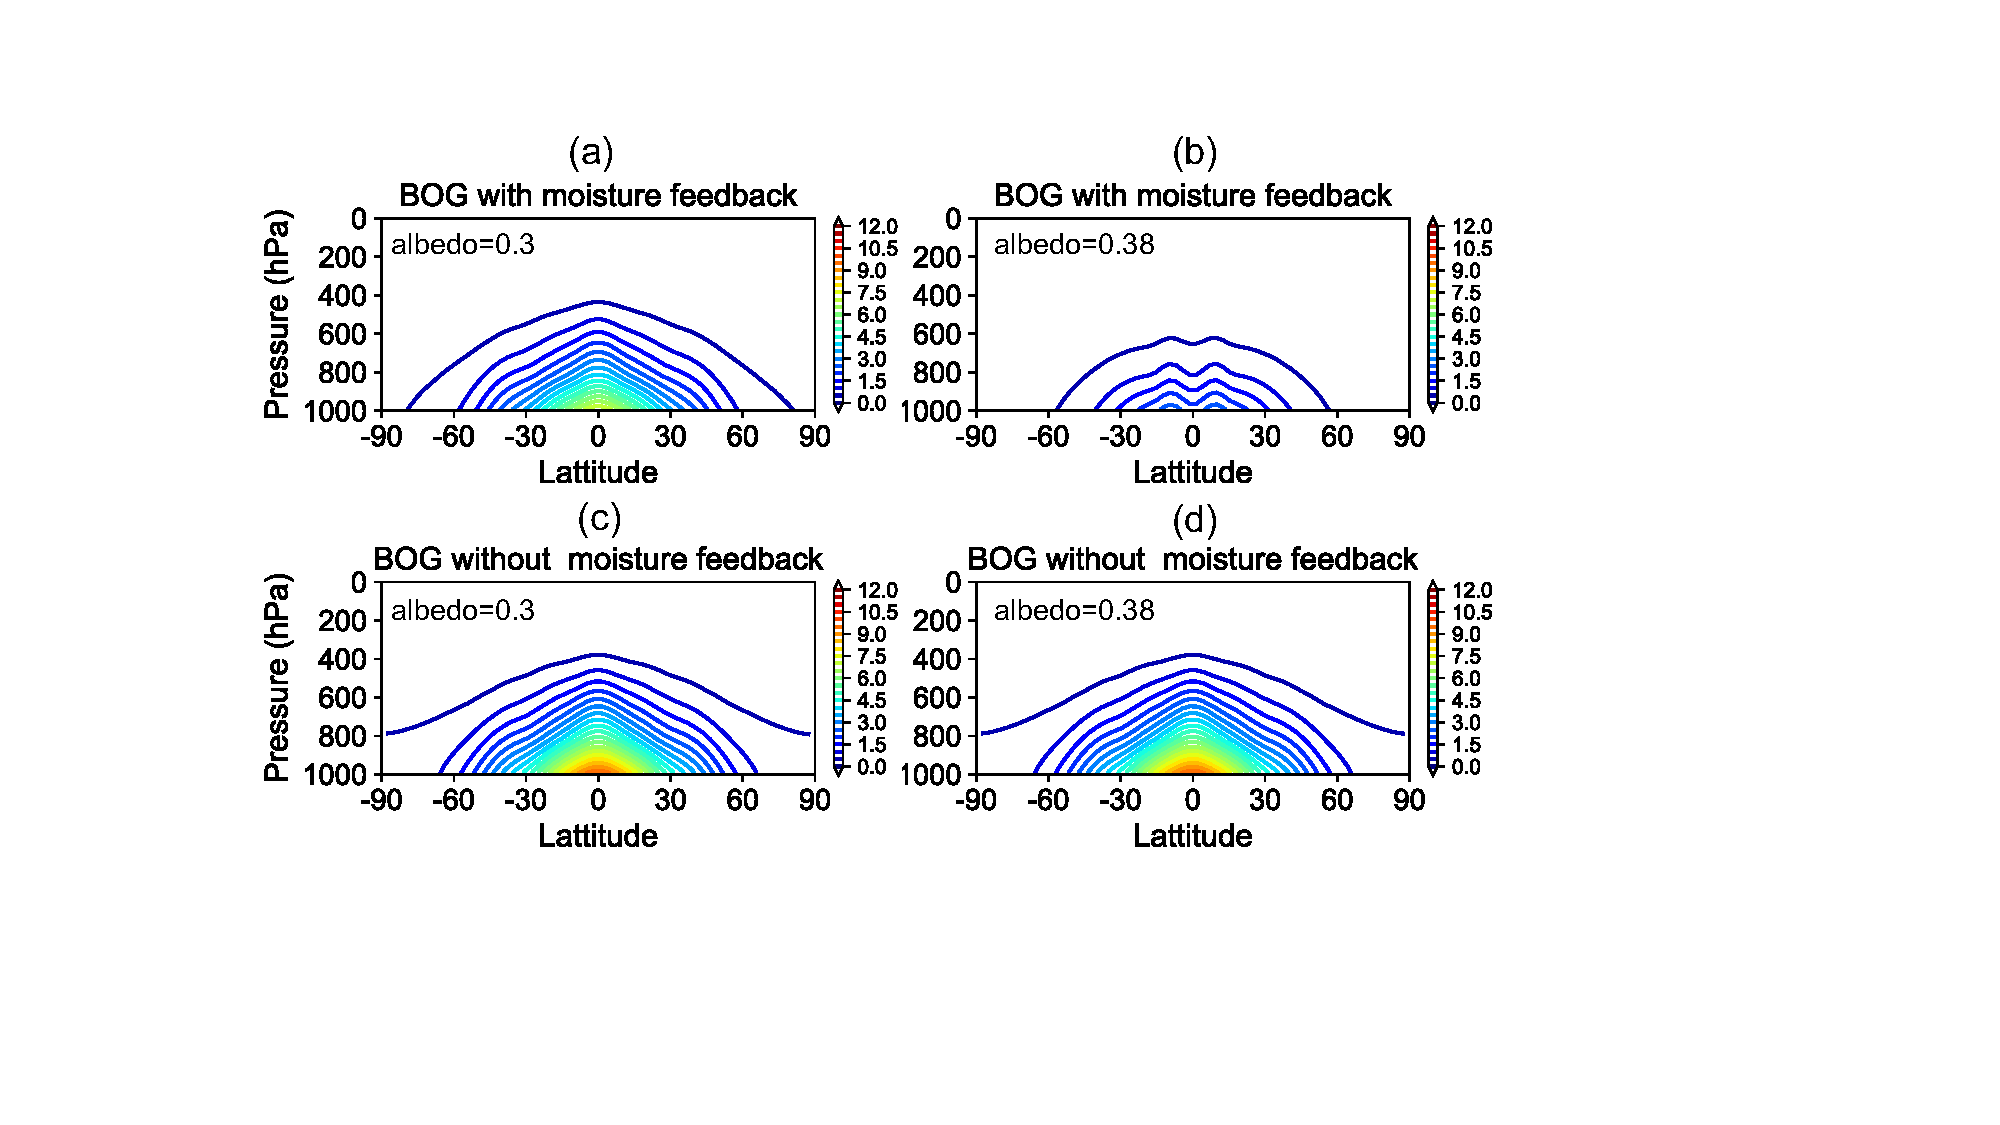
\includegraphics[width=0.8\textwidth]{{figs/polar_amp/lw_optical_depth}.pdf}
	\caption[Annual and zonal mean longwave optical depth in the BOG radiation scheme before and after reading the $q$ profile.]{Annual and zonal mean longwave optical depth in the BOG radiation scheme before and after reading the $q$ profile. (a) and (b) are the averaged longwave optical depth from the experiments with moisture feedback where albedo is 0.3 and 0.38. (c) and (d) are similar to (a) and (b), but the $q$ profiles are fixed by reading annual and zonal mean $q$ profile from control experiment (aledo is 0.3), so (c) and (d) are identical with each other.}
	\label{fig:optical_depth}
\end{figure}

To identify the role of moisture feedback in the BOG radiation scheme, we read the specific humidity ($q$) profile from the control run (i.e. $\alpha=0.3$) into other experiments (i.e. $\alpha=0.38$, $0.33$ and $0.27$) to make the moisture feedback fixed in the longwave radiation transfer. The longwave optical depths are examined first before analyzing the simulation results. For instance, the original optical depth profiles from the two runs where albedos are 0.3 (\figref{fig:optical_depth}a) and 0.38 (\figref{fig:optical_depth}b) show great differences when the moisture feedback is freely performed in radiation schemes, but they are almost identical to each other after the specific humidity profile for the run where albedo is 0.38 has been specified by the profile from control experiment (\figref{fig:optical_depth}c and \ref{fig:optical_depth}d). Compared to the original optical depths, the runs with increased albedos (e.g. $\alpha=0.38$) have thicker optical depths as they have been prescribed with specific humidity profiles from a warmer control state ($\alpha=0.3$), where the atmospheric water vapor content is much larger due to the non-linear effect of saturation water vapor pressure with respect to temperature according to Clausius-Clapeyron relation. Similarly, the runs with decreased albedos will have a thinner optical depth as they are specified with moisture profiles from relative cold control state.

%Normally, temperature increases when albedo is changed from 0.38 to 0.3, and thus , meaning that the longwave optical depth becomes larger as albedo declines. In regard to the case where albedo is 0.3, the optical depth increasing slightly, which is normal because the water vapor content has to increase gradually with the temperature going up, but the moisture content is always high when the experiment is prescribed with the annually averaged specific humidity profile.
%as they are prescribed with the same specific humidity profile. 
%of experiment where albedo is 0.38 has been specified by the optical thickness from control experiment (\figref{fig:optical_depth}), where the optical depths in \figref{fig:optical_depth}c and \figref{fig:optical_depth}d are almost identical as they are prescribed with the same specific humidity profile. 
% SURFACE TEMPERATURE AND THIR CHANGE when no moisture feedback in the BOG
% while the optical depth for control experiment doesn't change too much.

%\begin{table}[ht]
%	\centering
%	\caption{there is no moisture feedback in the BOG radiation scheme.}
%	\begin{adjustbox}{center=\textwidth}
%		\begin{tabular}{l c c c}
%			\toprule
%			\multirow{2}{*}{Region} & \multicolumn{3}{c}{Byrne(albedo=$x$-ctrl)}  \\
%			\cline{2-4}  
%			& $x$=0.38 & $x$=0.33 & $x$=0.27\\
%			\midrule
%			Arctic & -5.62 & -2.23 & 2.03 \\
%			Globe & -4.64 & -1.71 & 1.67 \\
%			$\Delta T_A/\Delta T_G$ & 1.21 & 1.31 & 1.22\\
%			\bottomrule
%		\end{tabular}
%	\end{adjustbox}
%	\label{tab:arctic_global_warming_ratio_no_wv}
%\end{table}

The surface temperature change for the BOG radiation scheme without moisture feedback (BOG-qctrl, orange dash-dotted lines in \figref{fig:delta_ts}) shows different behaviors from the runs with water vapor feedback, where the zonal mean surface temperature changes are much smaller and polar amplification becomes much weaker compared to the original runs. This indicates that the moisture feedback plays an important role in the surface temperature change as well as polar amplification at least in the BOG scheme. Note that the surface temperature changes in the runs without moisture feedback in the BOG scheme are close to those in the Frierson scheme, which is reasonable as the moisture feedback is also missing in the Frierson scheme. In addition, the vertical temperature profiles in polar and tropical regions also change a lot when there is no water vapor feedback in the BOG scheme. Specifically, the bottom-heavy cooling or warming profiles become less evident in polar region (see the orange dash-dotted lines in \figsref{fig:delta_t_profile}a-c) and the top-heavy cooling or warming profiles get weaker in tropical region (orange dash-dotted lines in \figsref{fig:delta_t_profile}d-f), implying the positive lapse rate feedback is weakened in polar region.

%To find out the outcome in the BOG radaition scheme without moisture feedback, we turn to the changes of surface temperature with various albedos. As shown in \tabref{tab:arctic_global_warming_ratio_no_wv}, the changes of Arctic and global mean surface temperature when changing albedos have decreased drastically compared to the ones in the experiments with allowing moisture feedback. In addition, the polar amplification of surface temperature in the BOG scheme without moisture feedback is no longer evident, and the ratios of surface temperature changes in Arctic and globe become close to the ones from the Frierson scheme (shown in \tabref{tab:arctic_global_warming_ratio}). 

%Whta's more, the northward heat transports resemble to each other (\figref{fig:ht_bog_no_wv_fb}) and the abnormal behaviours, such as reversals in latent heat transport and Hadley cell circulation (\figref{fig:hadleycell_no_moisture}), in the experiment where albedo is 0.38 also disappear when there is no moisture feedback in the BOG radiation scheme. All the facts above indicate that the moisture feedback plays an important role in the change of surface temperature as well as polar amplification when adopting different albedos in the BOG scheme. 

%\begin{figure}[ht]
%	\centering
%	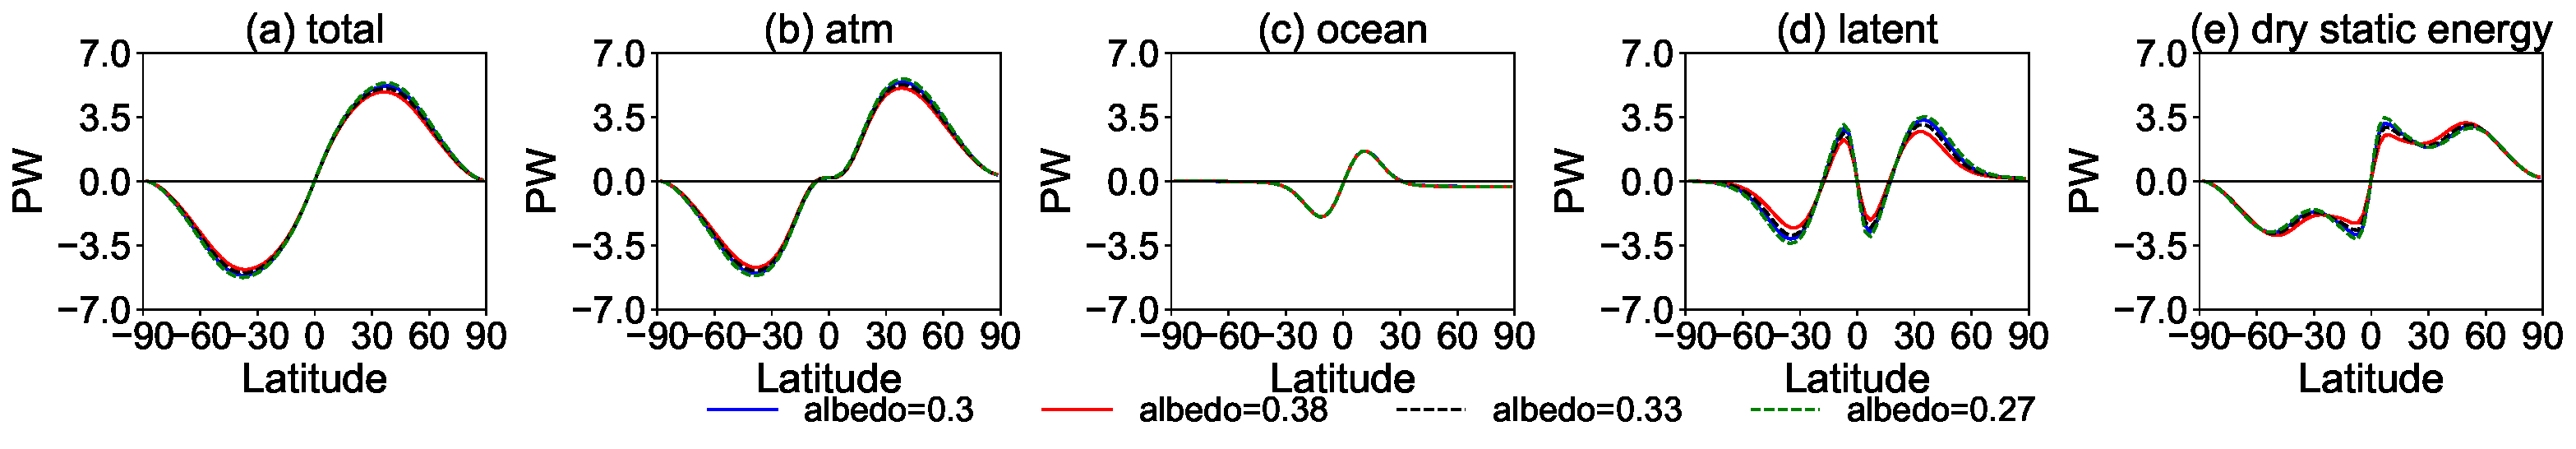
\includegraphics[width=1.0\textwidth]{figs/polar_amp/ht_bog_no_moisture.pdf}
%	\caption{As the transport for the BOG scheme in \figref{fig:ht_transport}, but no moisture feedback there.}
%	\label{fig:ht_bog_no_wv_fb}
%\end{figure}
%
%\begin{figure}[ht]
%	\centering
%	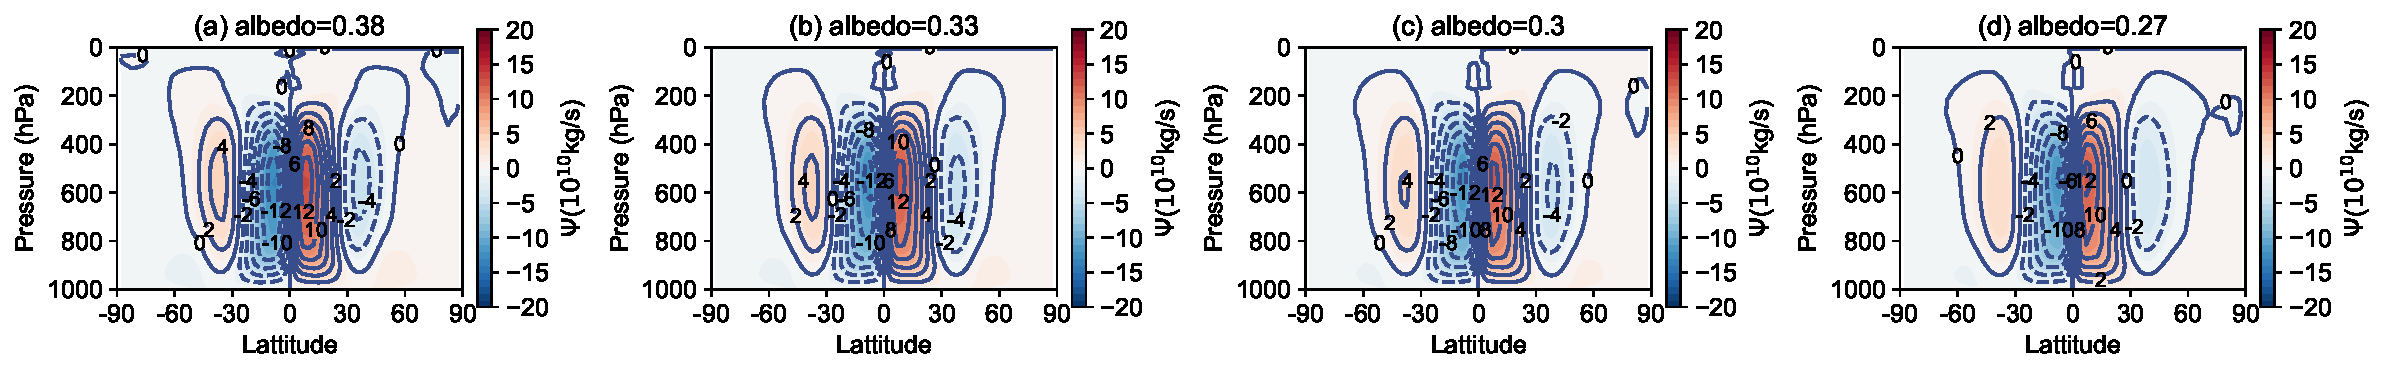
\includegraphics[width=1.0\textwidth]{figs/polar_amp/compare_bog_moisture_feedback/hadley_cell_bog_without_moisture_feedback.pdf}
%	\caption{As in \figref{fig:haleycell_bog}, but there is no moisture feedback in the BOG radiation scheme.}
%	\label{fig:hadleycell_no_moisture}
%\end{figure}
%
%However, there is still slight polar amplification even when there is no moisture feedback in the BOG radiation scheme when changing albedos as shown by $\Delta T_A/\Delta T_G$ in \tabref{tab:arctic_global_warming_ratio_no_wv}. Recall that the relationship between northward heat transport and surface temperature changes in Arctic and global areas has been discussed in \secref{sec:ht_hadley}, here the linkage is affirmed again. \figref{fig:ht_diff_bog_no_wv_fb} displays the differences of heat transport when changing albedos in the BOG radiation scheme without moisture feedback. Similarly, the differences of regional mean surface temperature both in Arctic and globe are approximately proportional to the differences of maximum of northward latent heat transport (\figref{fig:deltaT_lht_no_wv_fb}), which can be used to explain the slight polar amplification when changing albedos in the BOG radiation scheme even without moisture feedback.
%
%\begin{figure}[ht]
%	\centering
%	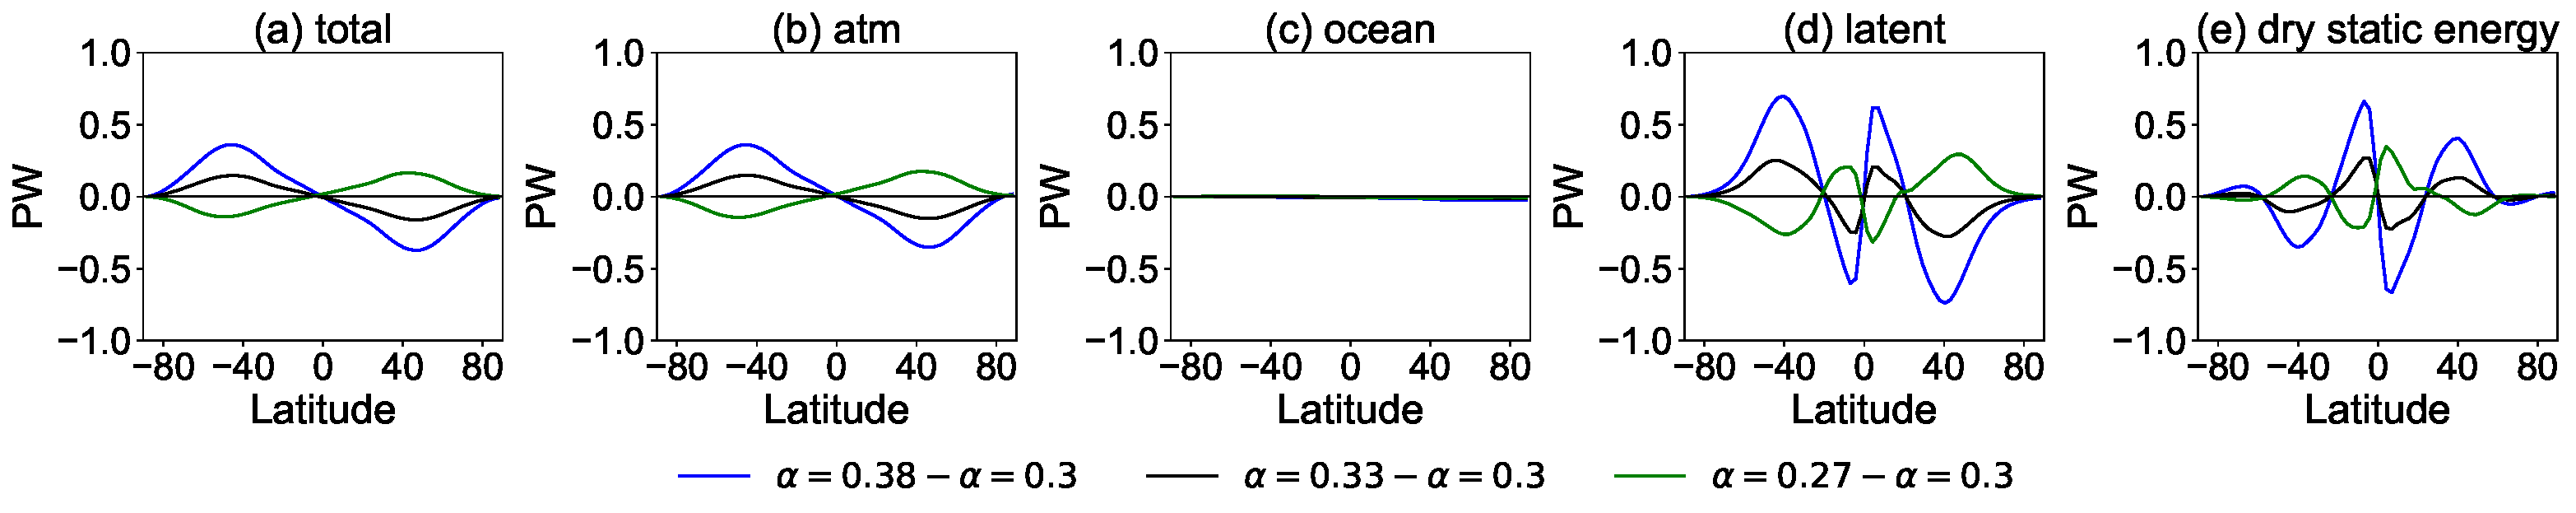
\includegraphics[width=1.0\textwidth]{figs/polar_amp/compare_bog_moisture_feedback/ht_diff_bog_no_moisture.pdf}
%	\caption{As the difference of heat transport for the BOG scheme in \figref{fig:ht_transport_diff}, but no moisture feedback in these experiments.}
%	\label{fig:ht_diff_bog_no_wv_fb}
%\end{figure}
%
%\begin{figure}[ht]
%	\centering
%	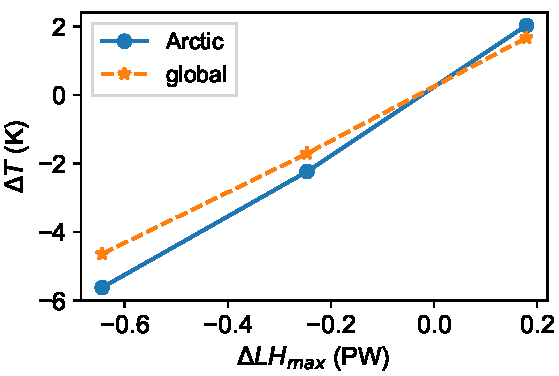
\includegraphics[width=0.5\textwidth]{figs/polar_amp/linear_relation_Delta_T_ht_no_moisture_bog.pdf}
%	\caption{The relationship between the differences of regional mean surface temperature and the differences of maximum of northward latent heat transport in the BOG radiation scheme without moisture feedback.}
%	\label{fig:deltaT_lht_no_wv_fb}
%\end{figure}
%

\begin{figure}[ht]
	\centering
	\makebox[\linewidth]{
	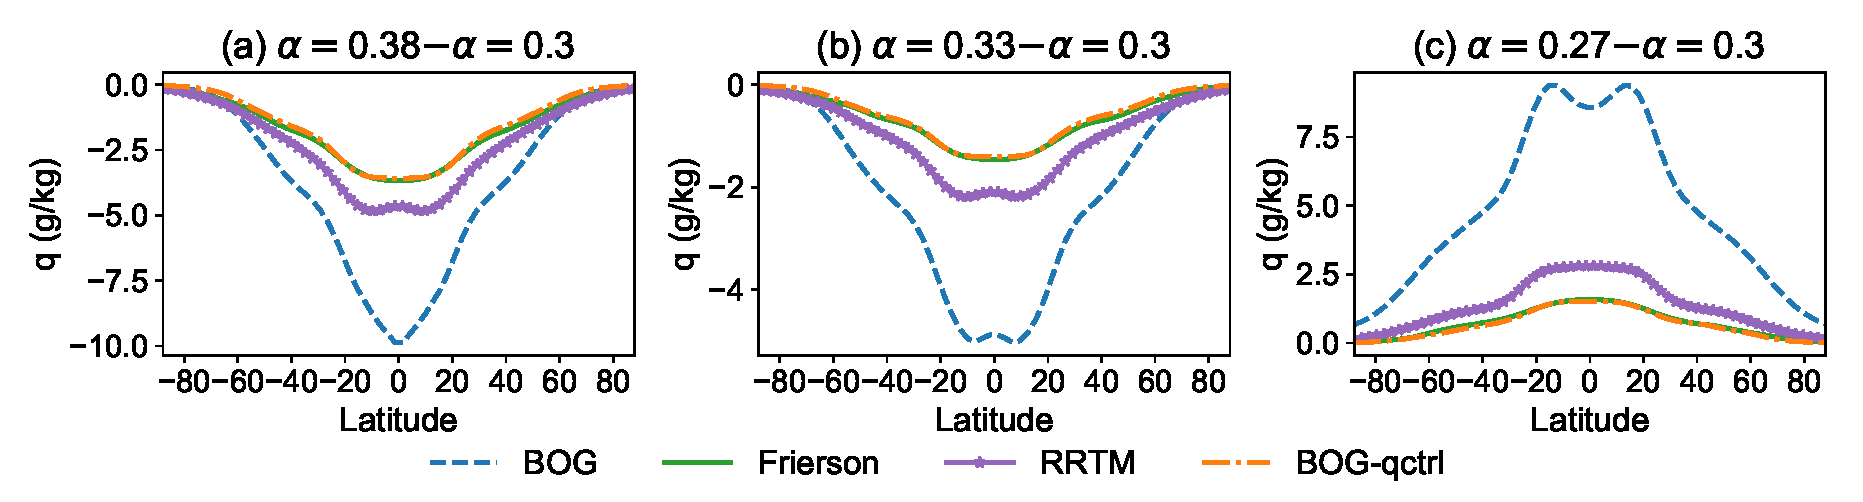
\includegraphics[width=1.1\textwidth]{figs/polar_amp/sfc_q_diff_gradient}}
	\caption[The zonal and annual mean specific humidity changes]{As in \figref{fig:delta_ts}, but for the specific humidity at surface. }
	\label{fig:sfc_q_zonal}
\end{figure}

As remarked by \cite{Pithan2014}, the water vapor feedback contributes more to the tropical warming than to polar warming, which corresponds to our findings for the BOG radiation scheme (\secref{sec:climate_feedbacks_temp_decomp}). But we should also notice that while water vapor feedback does not result in polar amplification by itself, it could approximately double the climate sensitivity both at low and high latitudes \citep{Langen2012}. However, we find the polar amplification of surface temperature decreases remarkably after turning off the water vapor feedback, which as illustrated in \figref{fig:sfc_q_zonal} (blue dashed and orange dash-dotted lines). This is due to the water vapor content and its meridional gradient, which have both changed when the moisture feedback is turned off. In addition, the zonal mean profile from BOG scheme with moisture feedback is quite different from the RRTM scheme, suggesting that the moisture feedback prescribed in the BOG radiation scheme is possibly too strong compared to a more realistic radiation scheme. Although the water vapor is only specified in radiation code, other processes associated with the advection and latent heat release are still retained in the BOG experiment, that is why the runs without moisture feedback (BOG-qctrl) behave so similarly to Frierson scheme. As illustrated in \figref{fig:tsurf_diff}, there is still slight amplified surface temperature change at high latitudes even if no moisture feedback is included in radiation schemes, and therefore other mechanisms need to be investigated.

% However, it is the unreasonable meridional water vapor gradient from tropics to pole that amplify the surface temperature change in high latitudes.

%But we found at least in the BOG radiation scheme, the moisture feedback plays a significant role in the surface temperature changes, where the polar amplification decreases largely without moisture feedback, which gives the causes to the differences between BOG and Frierson radiation scheme. In addition, there is 

%% --------------- Heat Transport ----------------- %%
\subsection{Heat transport}
\label{sec:heat_transport}

%The heat transports in all experiments will be analyzed to discern the roles of different components.
%For instance, considering the difference in the BOG and Frierson radiation schemes, the latent heat transport will be focused on in particular as water vapor is related to the latent heat release. 
 
The total northward energy transport $H$ across each latitude ($\varphi$) is calculated by the energy budget balance in an atmospheric column,
\begin{equation}
	H(\varphi) =  \int_{-\frac{\pi}{2}}^{\varphi}2\pi a^2(\text{ASR}-\text{OLR})\operatorname{cos}\varphi \operatorname{d}\varphi,
\end{equation}  
where $a$ is the radius of Earth, $\text{ASR}$ is the absorbed solar radiation flux and $\text{OLR}$ is outward longwave radiation flux at latitude band, and hence $\text{ASR}-\text{OLR}$ is the net TOA radiation. The total northward energy transport can be decomposed into energy transport by atmosphere and ocean. In our aquaplanet experiments, there is no Q-flux to represent the ocean heat transport, so the total energy transport is contributed from atmospheric energy transport ($H_{a}$, AET) only:
\begin{equation}
	H_a(\varphi) = H(\varphi).
\end{equation}
%In our aquaplanet experiments, a Q-flux is added as the oceanic heat transport, which is the same in all experiments and thus has no effect to the temperature responses after changing abledos. 

%Therefore, the northward oceanic energy transport $H_o$ is
%\begin{equation}
%H_o(\varphi)= -2\pi a^2\int_{-\frac{\pi}{2}}^{\varphi}\operatorname{cos}\varphi F_s\operatorname{d}\varphi,
%\end{equation}  and atmospheric energy transport $H_a$ is 
%\begin{equation}
%	H_a(\varphi)= 2\pi a^2\int_{-\frac{\pi}{2}}^{\varphi}\operatorname{cos}\varphi  (ASR-OLR+F_s)\operatorname{d}\varphi,
%\end{equation}  
%where $F_s$ represents the surface energy budget and is given by 
%\begin{equation}
%	Fs=SW+LW-SH-LH+\nabla \cdot \bm Q,
%\end{equation}
%in which $SW$ and $LW$ are the net shortwave and longwave radiation flux at surface, $SH$ is the sensible heat flux, $LH$ is the latent heat flux and $\bm Q$ is the Q-flux. 
In addition, the northward AET can be decomposed further into latent heat transport ($H_{LH}$), which is related to latent heat release, and dry static energy transport ($H_{dry}$) associated with the motion of dry air, which are given by 
\begin{equation}
	H_{LH}(\varphi)= 2\pi a^2\int_{-\frac{\pi}{2}}^{\varphi}\operatorname{cos}\varphi  L_v(E-P)\operatorname{d}\varphi,
\end{equation}
and 
\begin{equation}
H_{dry}=H_a-H_{LH},
\end{equation}
where $E$ and $P$ denote evaporation and precipitation respectively, and $L_v$ is the specific latent heat capacity. The meridional energy transports mentioned above in all experiments for the BOG, Frierson and RRTM radiation schemes are shown in the \figref{fig:ht_transport} and the changes of energy transport after changing albedos are displayed in \figref{fig:ht_transport_diff}.

\begin{figure}[ht]
	\centering
	\makebox[\linewidth]{
	%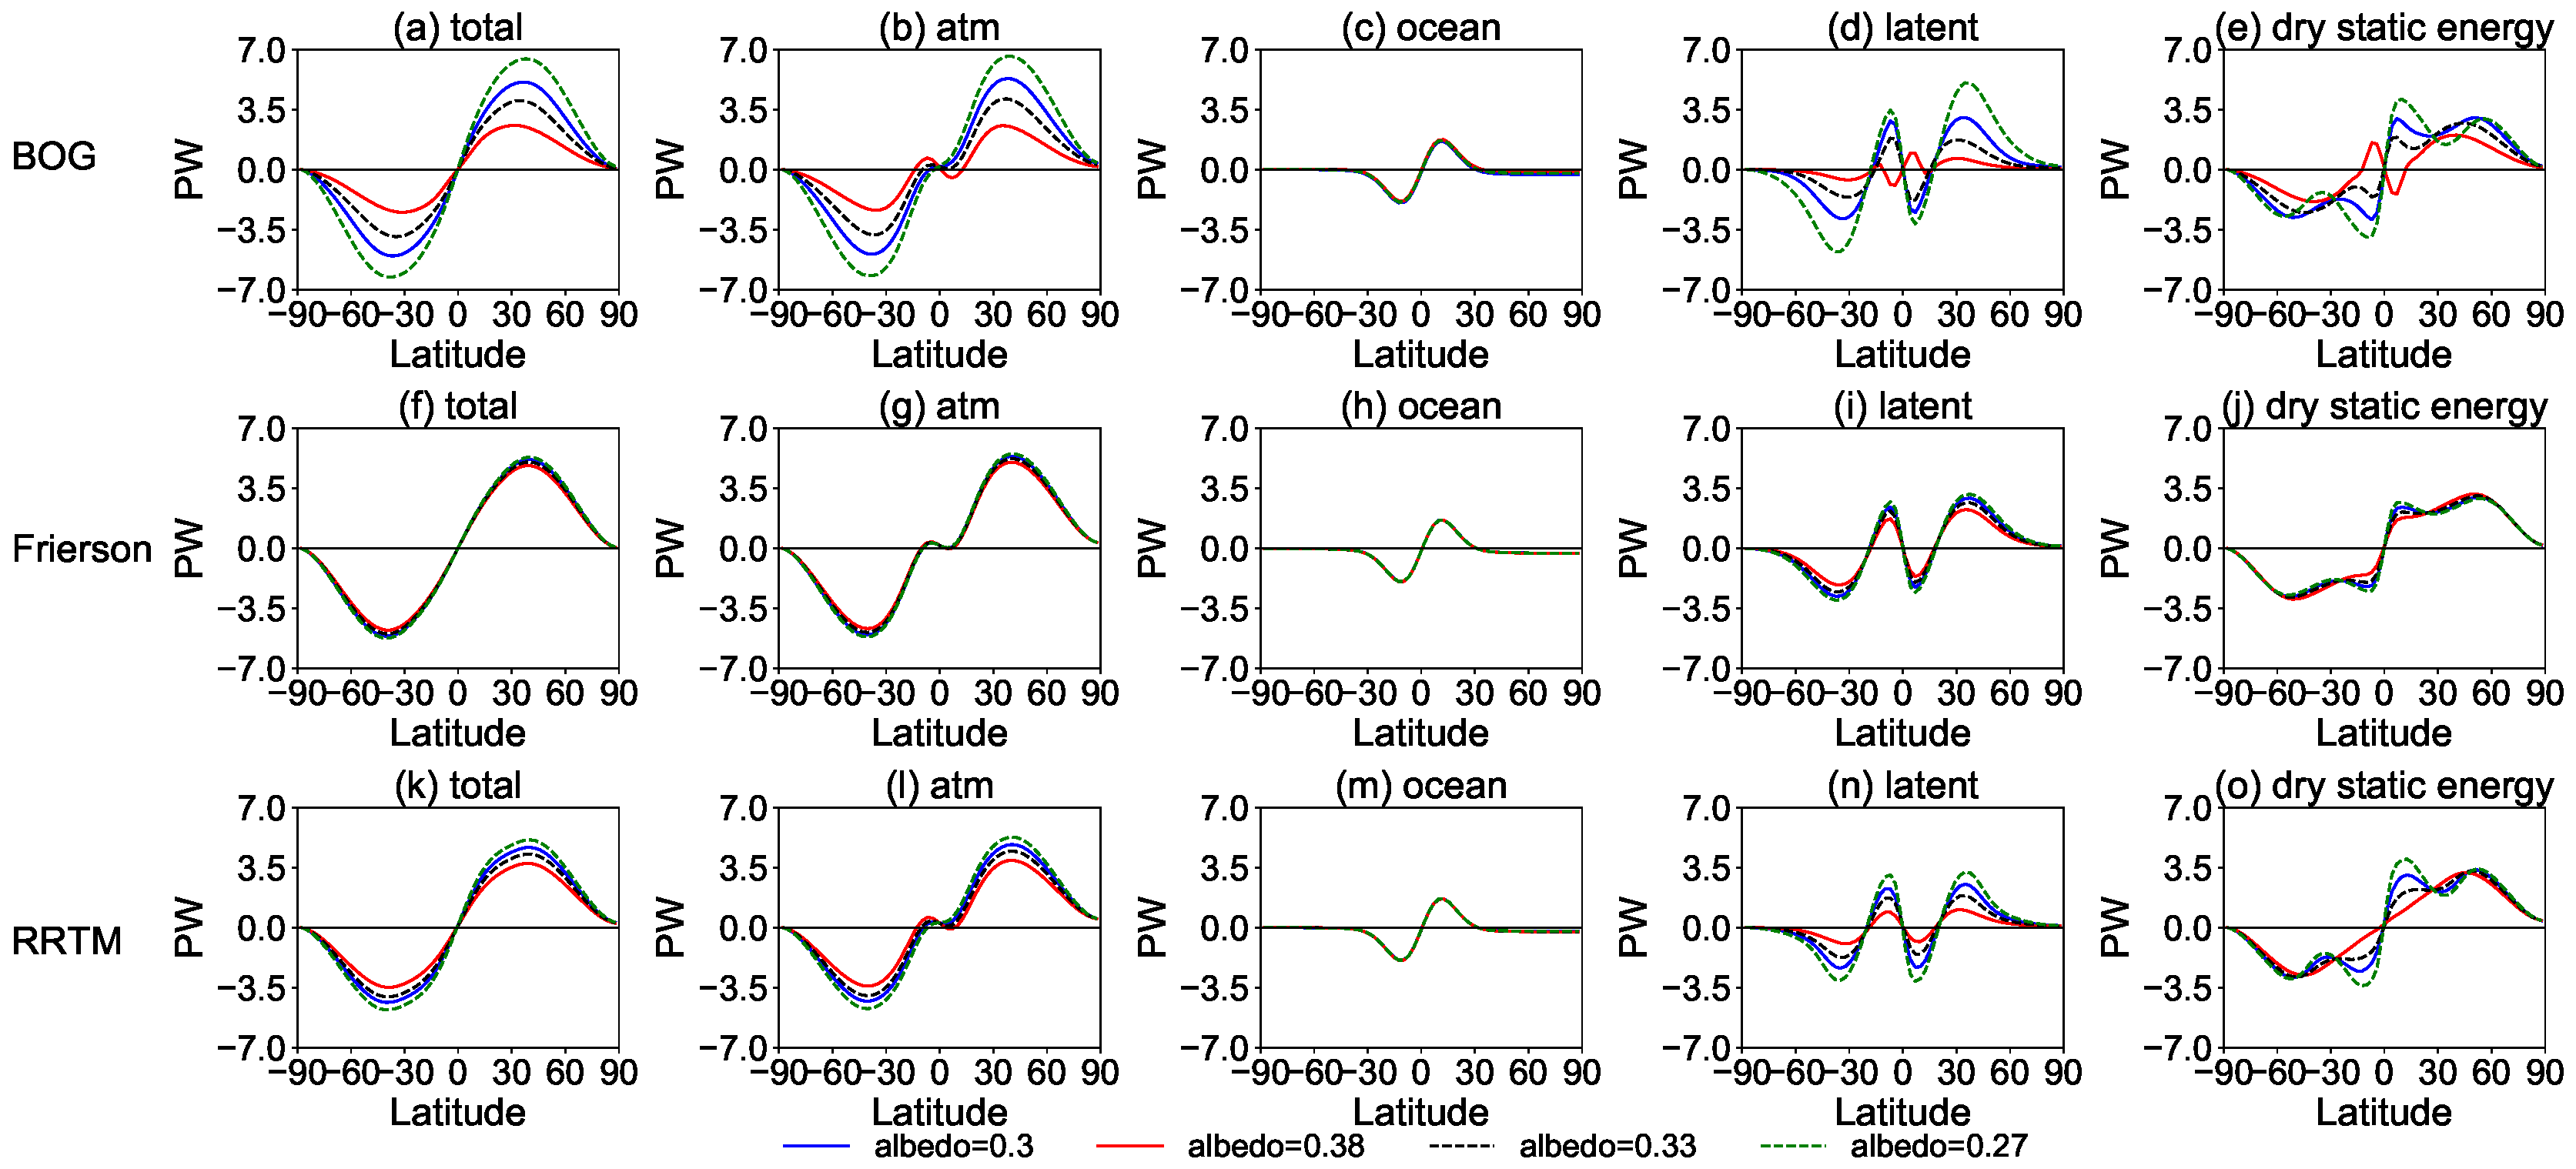
\includegraphics[width=1.1\linewidth]{{figs/polar_amp/poleward_ht_diff_compnts_diff_schemes_0.3_0.38_0.33_0.27}.pdf}}
	% \caption{Heat transport in the experiments with different radiation schemes and various albedos. The top, middle and bottom panels are for the BOG, Frierson and RRTM radiation schemes respectively. Total northward heat transports are shown in (a), (f) and (k), the atmospheric heat transports are presented in (b), (g) and (l), the oceanic heat transport related to Q-flux are listed in (c), (h) and (m), the latent heat transport are illustrated in (d), (i) and (n), and the dry static energy transport are depicted in (e), (j) and (o). Blue solid, red solid, blue dash and green dash lines indicate the experiments where albedos are 0.3, 0.38, 0.33 and 0.27 respectively.}
	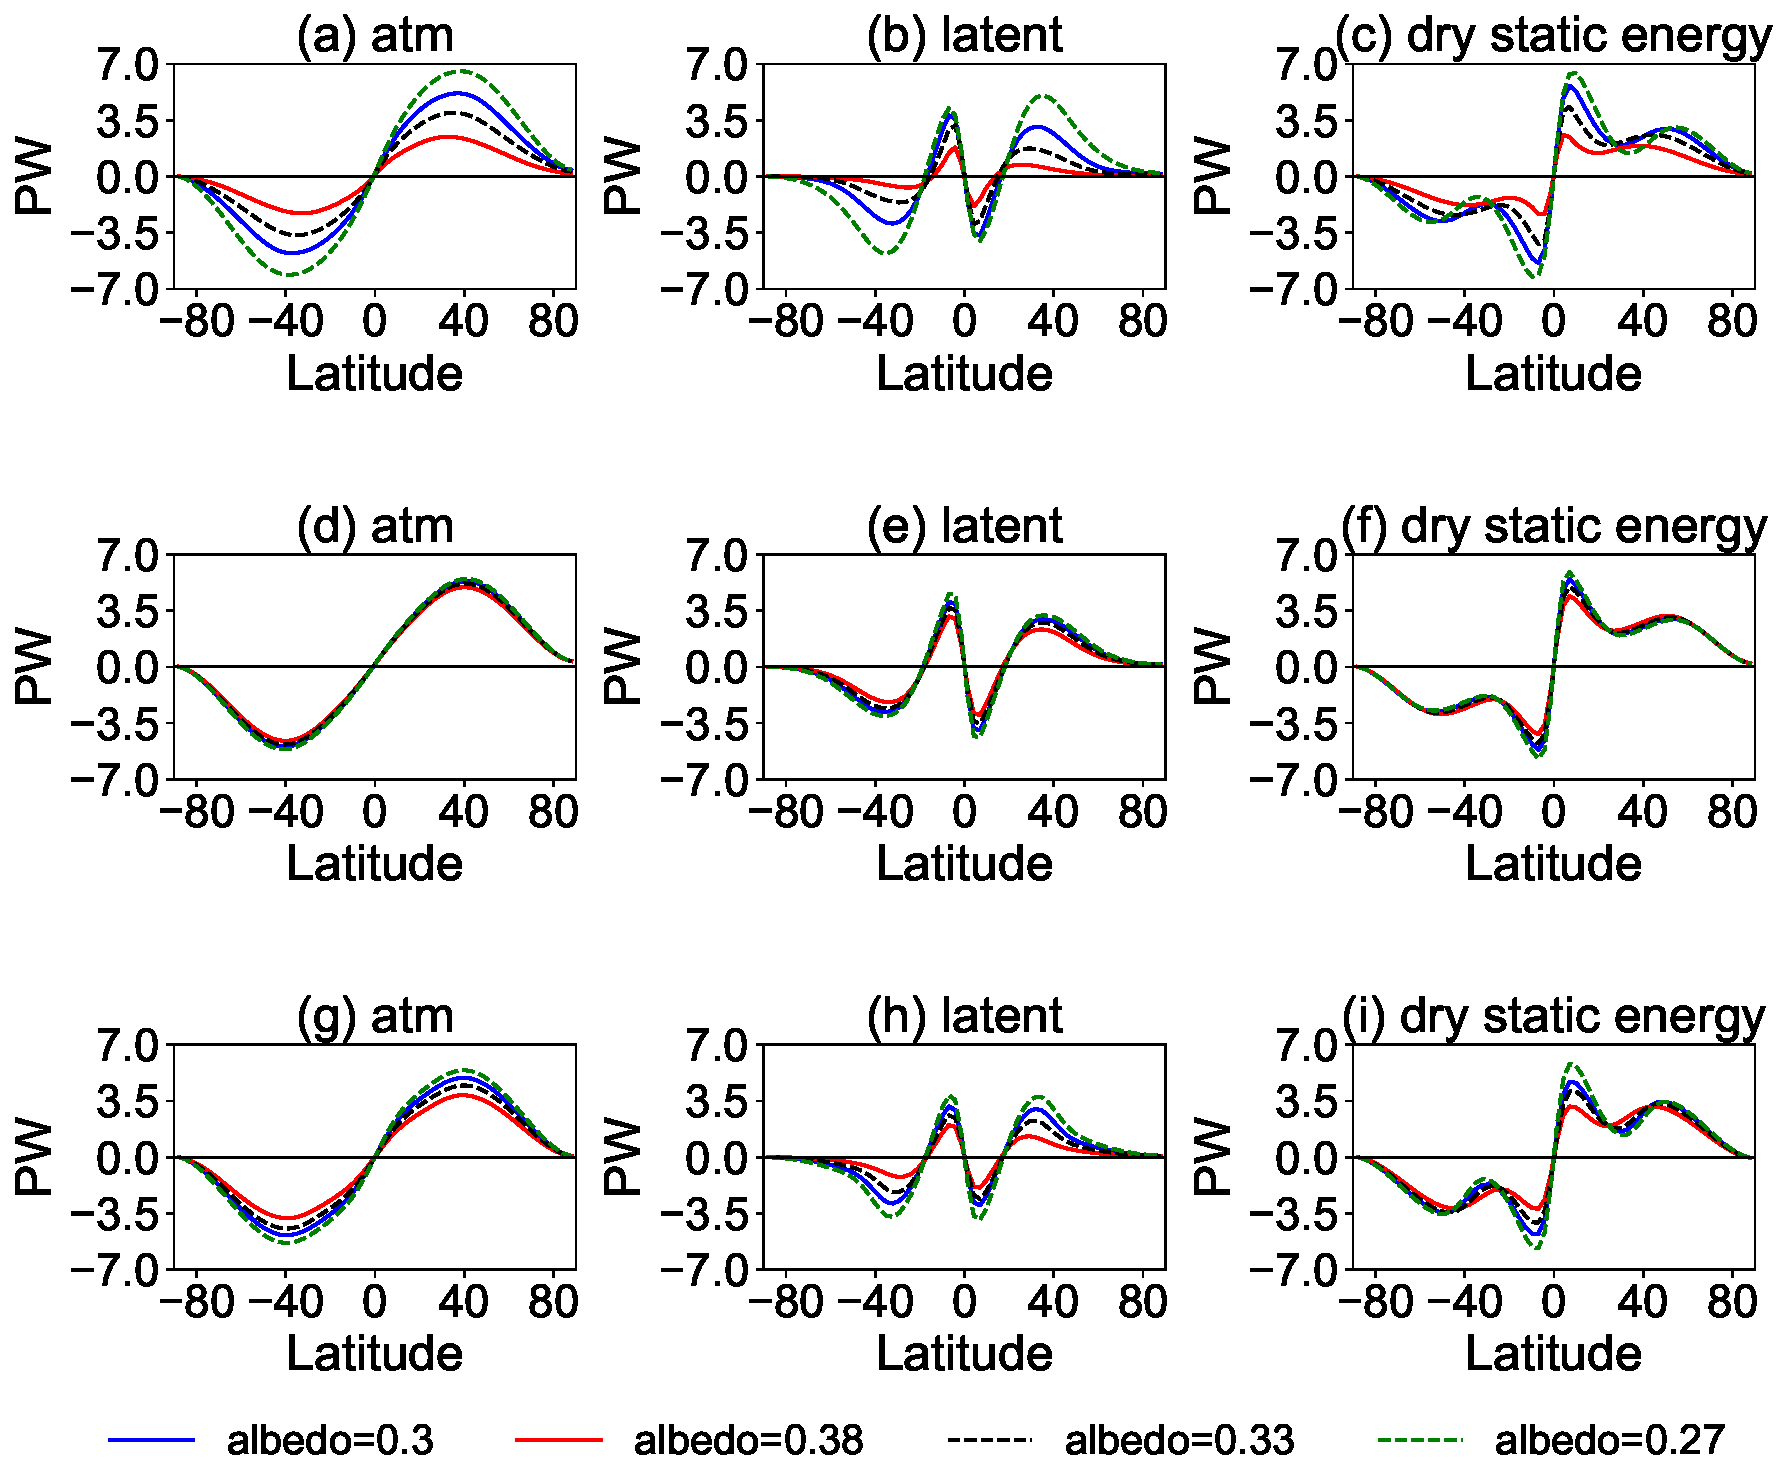
\includegraphics[width=0.9\linewidth]{{figs/polar_amp/poleward_ht_diff_compnts_diff_schemes}.pdf}}
    \caption[Heat transport in the experiments with different radiation schemes and various albedos]{Heat transport in the experiments with different radiation schemes and various albedos. The top, middle and bottom panels are for the BOG, Frierson and RRTM radiation schemes respectively. The atmospheric heat transports are presented in (a), (d) and (g), the latent heat transport are illustrated in (b), (e) and (h), and the dry static energy transport are depicted in (c), (f) and (i). Blue solid, red solid, blue dash and green dash lines indicate the experiments where albedos are 0.3, 0.38, 0.33 and 0.27 respectively.}
	\label{fig:ht_transport}
\end{figure}

%$$\frac{\partial E_o}{\partial t} = -F_s- \frac{1}{2\pi a^2\operatorname{cos}\varphi}\frac{\partial H_o(\varphi)}{\partial \varphi}$$
%$$\frac{\partial E_a}{\partial t} = R_{TOA}+F_s- \frac{1}{2\pi a^2\operatorname{cos}\varphi}\frac{\partial H_a(\varphi)}{\partial \varphi}$$
%$$L_v\frac{\partial Q}{\partial t} = L_v(Evap-Precip)- \frac{1}{2\pi a^2\operatorname{cos}\varphi}\frac{\partial H_{LH}(\varphi)}{\partial \varphi}$$

%For the simulations with the BOG's radiation scheme, the TET shows large differences between the runs where the albedos are 0.38 and 0.3. The TET is composed of atmospheric and oceanic energy transport, and the oceanic energy transports are nearly the same (\figref{fig:ht_transport}c), so the main differences of TET are from the atmospheric energy transport (\figref{fig:ht_transport}b), most of which are contributed from latent heat transport (\figref{fig:ht_transport}d). However, all the energy transport for the simulations with Frierson's scheme are almost equal when changing the albedos, indicating that it is the moisture in the radiation scheme that leads to polar amplification in the experiments with the BOG's radiation scheme.


% In the aquaplanet setups, the mixed layer is prescribed with same Q-flux symmetric to the equator in the experiments, and thus the northward ocean heat transports in all experiments resemble to each other (\figsref{fig:ht_transport}c, h, m) and the differences when changing the albedos are nearly zero (\figsref{fig:ht_transport_diff}c, h, m). Therefore, the difference in total energy transport are from the atmospheric sources rather than from oceanic ones. 

The changes of the surface albedo do have influence on the atmopspheric energy transports in these experiments, although the degree of influence is different. The experiments performed with the BOG radiation scheme have the largest changes after varying the albedo, the runs with the RRTM radiation schemes have moderate changes, while the ones with Frierson schemes have the least effect (\figsref{fig:ht_transport}a, d and g), which are much clearer when checking the differences of the experiments in \figsref{fig:ht_transport_diff}. Compared to the dry static energy transport, the latent heat transport contributes a larger portion to the total atmospheric at 40$^\circ$ poleward (\figsref{fig:ht_transport} and \ref{fig:ht_transport_diff}). Previous studies have shown that an increase in atmospheric heat transport can cause midtropospheric warming in polar region \citep[e.g.,][]{Screen2012}, which can explain indirectly the polar amplification in the experiments under seasonal or annual mean insolations \citep{Kim2018}.  Here we also examined the temperature change in polar region ($70^\circ$ northward) both at surface and mid-troposphere (450-700hPa) (\figref{fig:delta_ht_ts}). The results show strong linear relationships between the total AET change across $70^\circ$ and either the surface temperature change and ($R^2=0.97$, \figref{fig:delta_ht_ts}a) or mid-troposphere temperature change ($R^2=0.90$, \figref{fig:delta_ht_ts}b), implying that the heat transport is associated with the polar amplification both at surface and mid-troposphere under insolation conditions.

% The results show strong linear relationships between the surface temperature change and the total AET change across $70^\circ$ ($R^2=0.98$, \figref{fig:delta_ht_ts}a) and between mid-troposphere temperature change and poleward AET at $70^\circ$ ($R^2=0.93$, \figref{fig:delta_ht_ts}b), implying that the heat transport is much possible associated with the polar amplification at surface.

%\cite{Feldl2017}
%because in the two cases the polar warming is largest in mid-troposphere rather than at surface.

%Furthermore, the differences of total or latent heat transport are largest in the BOG scheme, moderate in the RRTM scheme and least in the Frierson scheme, which seems to explain the varying levels of polar amplification in the three radiation schemes. In order to link the surface temperature change and polar amplification with the latent heat transport, the change of surface temperature after increasing or decreasing albedos are compared with the difference of maximum of northward latent heat transport, used as a proxy to represent the change of northward latent heat transport, in all the three radiations (\figref{fig:delta_ht_ts}). Strikingly, both the changes of Arctic and global mean of surface temperature due to various albedos have good linear relationships with changes of maximum of latent heat transport for all three radiation schemes, indicating that the changes of latent heat transport may explain the differences of global mean surface temperature as well as the polar amplification.

\begin{figure}[ht]
	\centering
	%\hspace{-1cm}
	%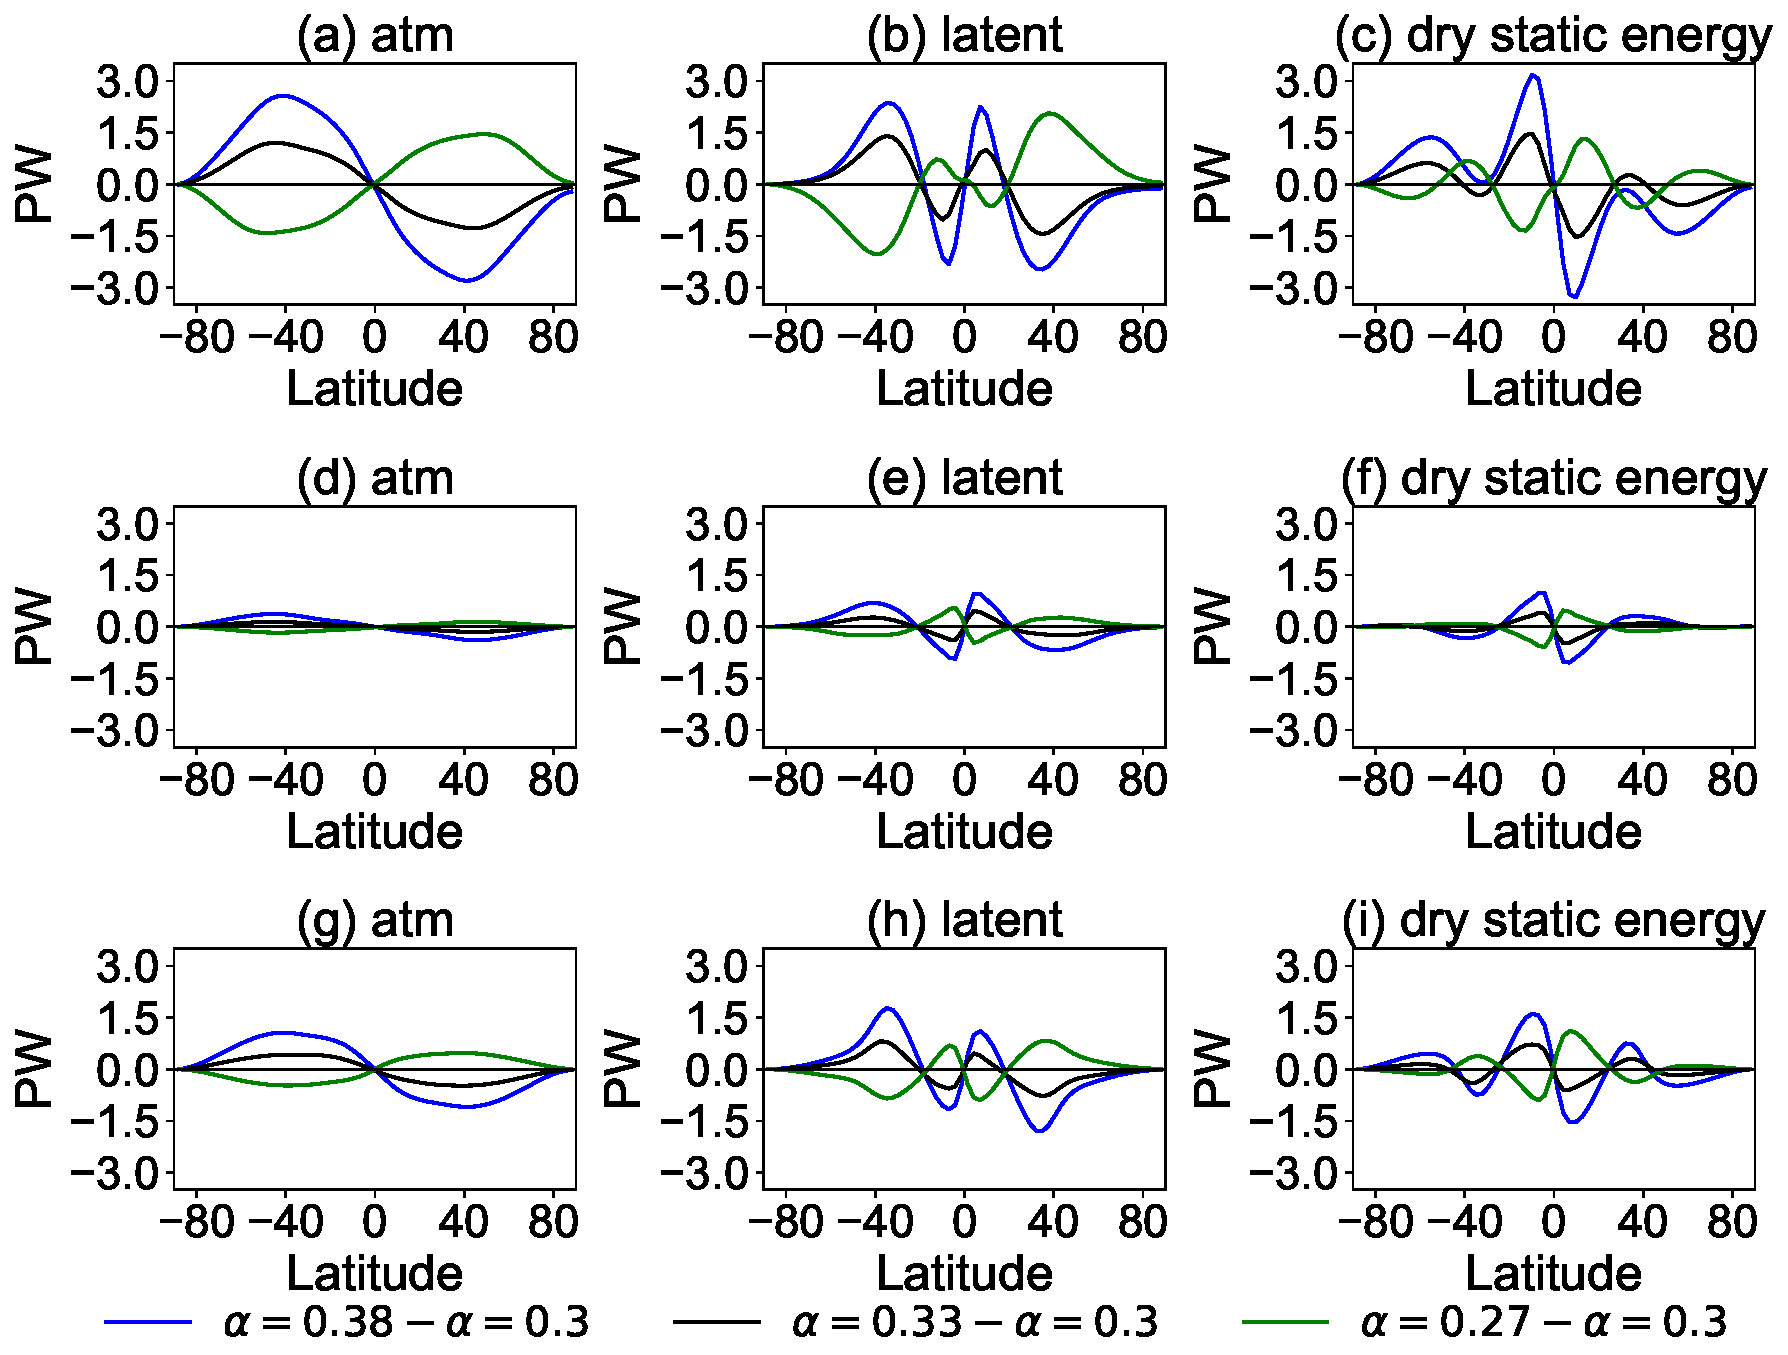
\includegraphics[width=1.\linewidth]{{figs/polar_amp/heat_transport_bog_frierson_components_diff_test}.pdf}
	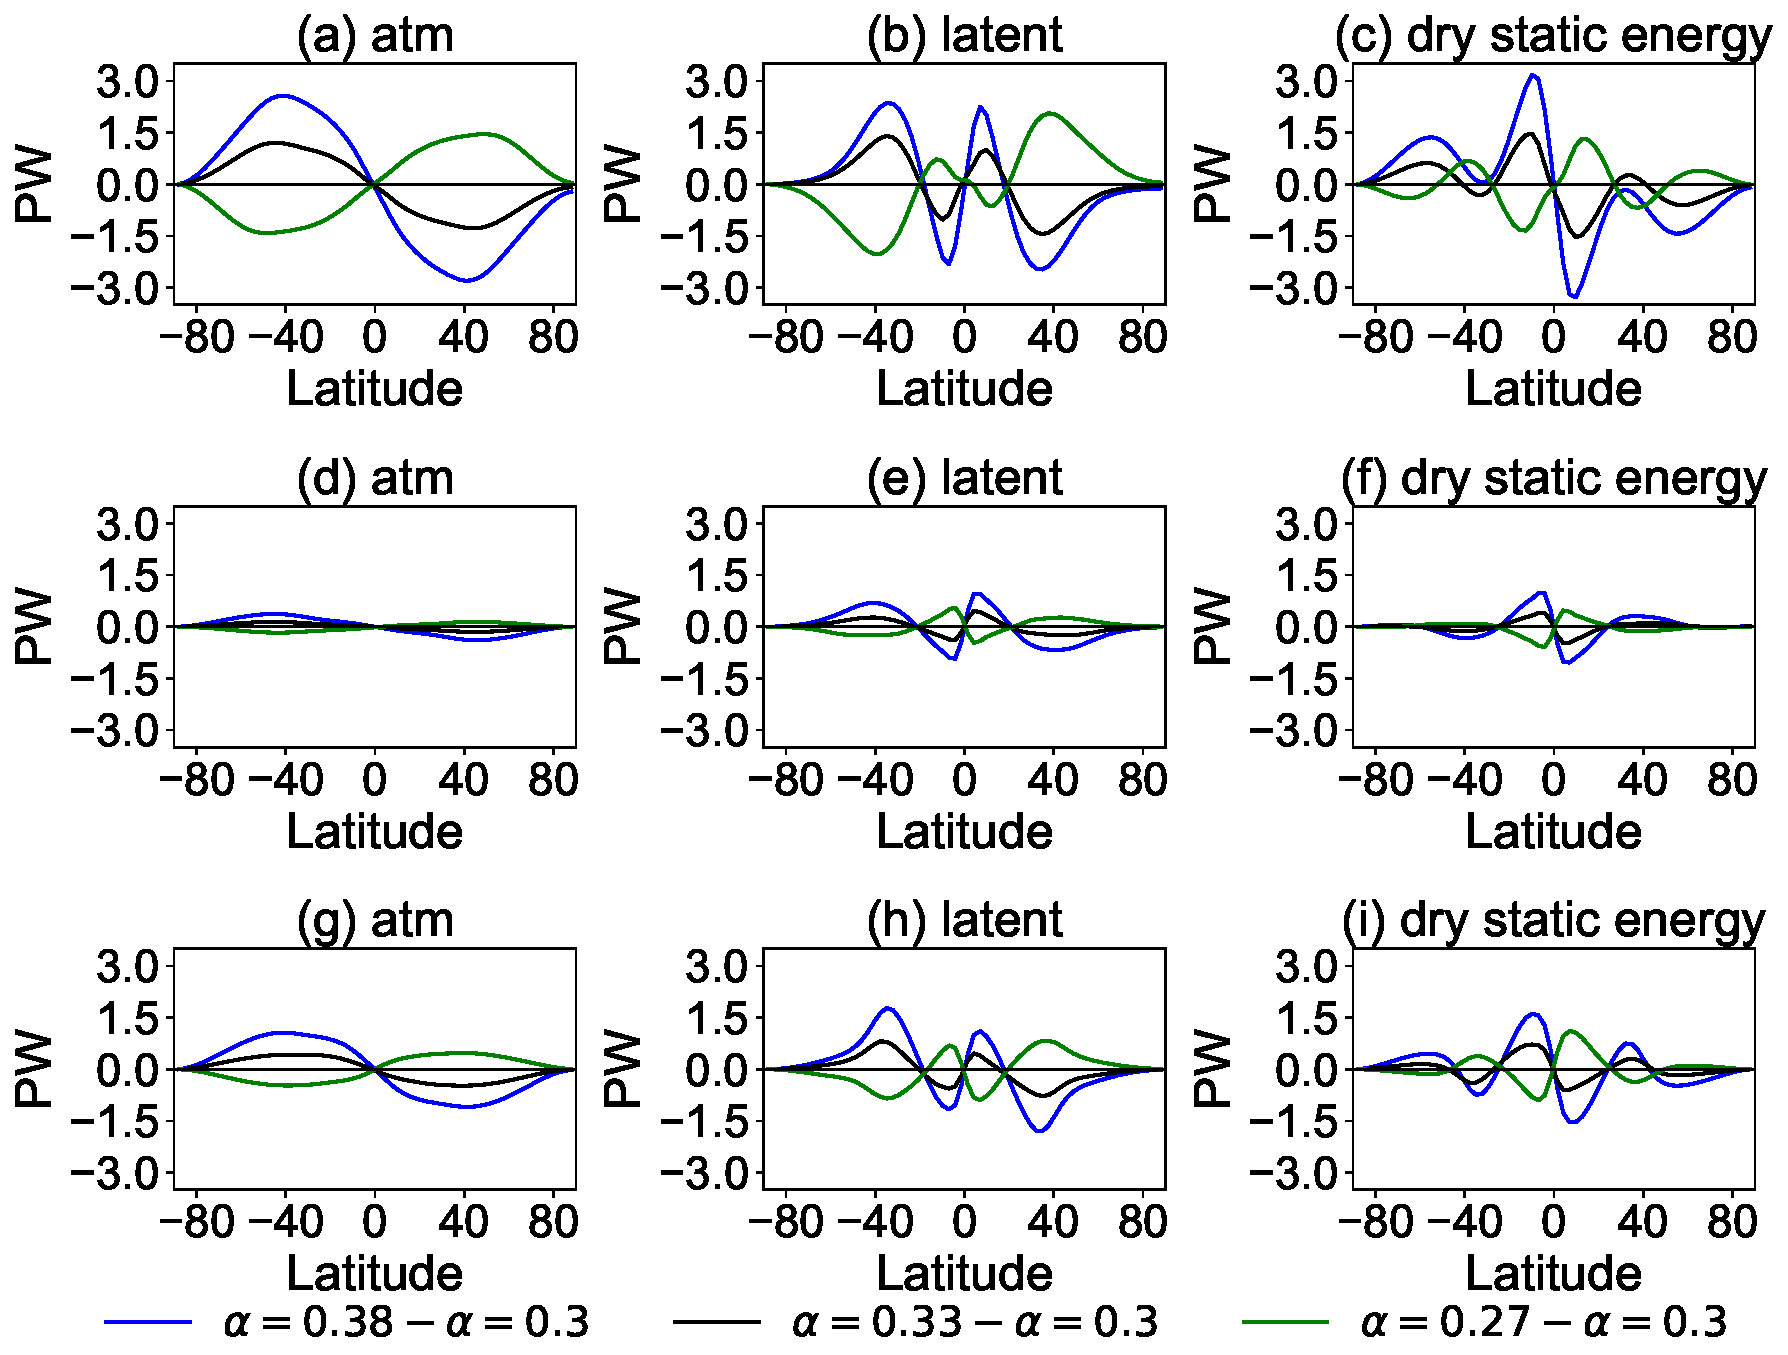
\includegraphics[width=0.9\linewidth]{{figs/polar_amp/heat_transport_bog_frierson_components_diff_test}.pdf}
	\caption[Changes in heat transport after varying the albedos]{As in \figref{fig:ht_transport}, but for the difference in heat transport between the experiments with different radiation schemes and various albedos. Blue, black and green solid lines indicates the difference between experiments where albedo is 0.38, 0.33 and 0.27 and the control experiment respectively.}
	\label{fig:ht_transport_diff}
\end{figure}

\begin{figure}[ht]
	\centering
	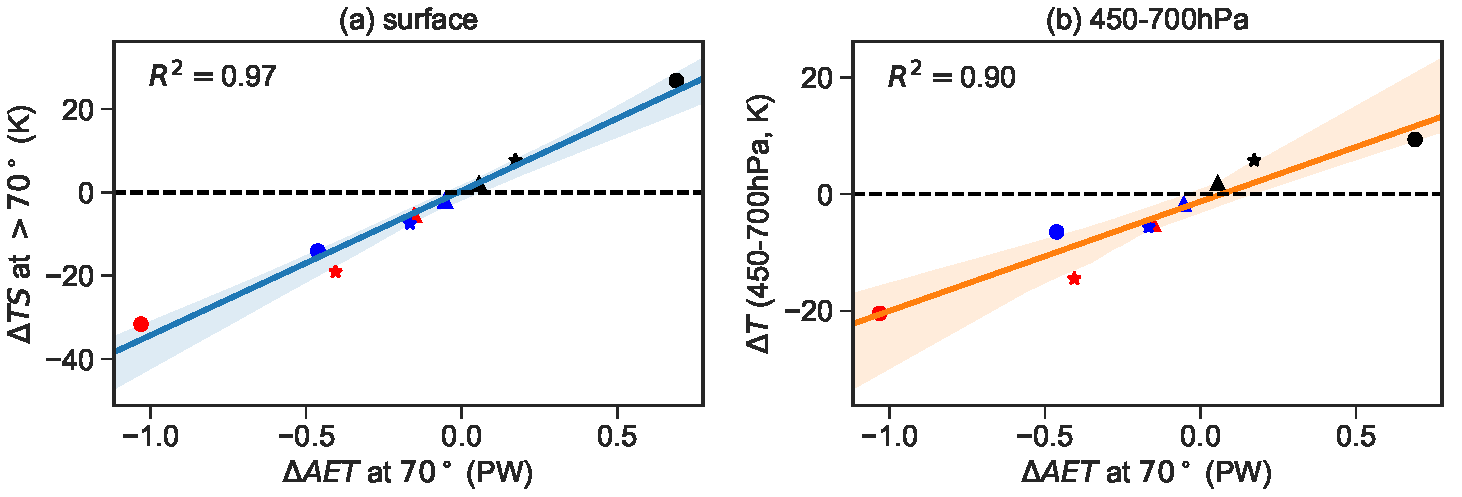
\includegraphics[width=0.8\linewidth]{figs/polar_amp/heat_transport_delta_ts.pdf}
	\caption[Changes of (a) surface temperature and (b) temperature at middle troposphere in polar region versus changes in atmospheric energy transport at $70^\circ$.]{(a) Changes of surface temperature poleward of $70^\circ$ versus changes in atmospheric energy transport (AET) at $70^\circ$ and the blue line is the linear regression of the two variables with the shading area indicating the 95\% confidence interval. The solid circles, stars and triangles denote the BOG, Frierson and RRTM schemes respectively, and red, blue and black markers represent the runs in which the albedos are changed from 0.3 to 0.38, 0.33 and 0.27 respectively. (b) Same as (a), but for temperature change in middle troposphere (450--700 hPa).}
	\label{fig:delta_ht_ts}
\end{figure}


%\begin{figure}[ht]
%	\centering
%	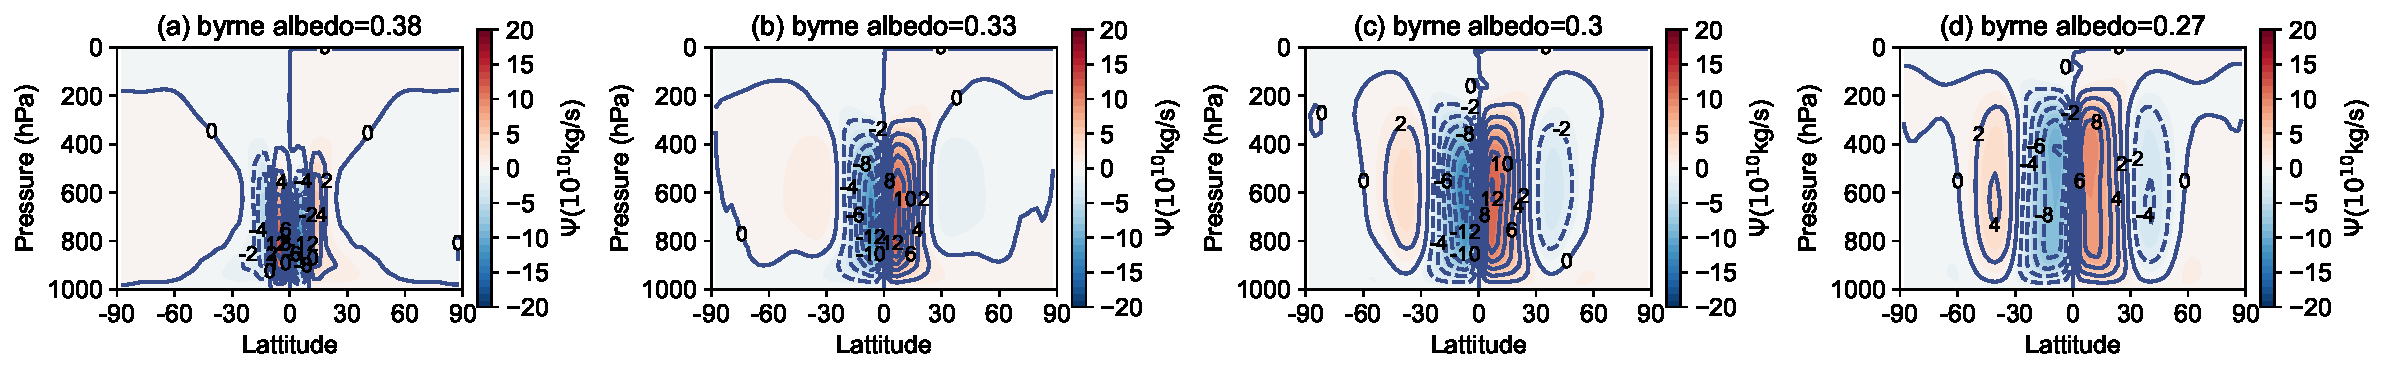
\includegraphics[width=1.0\linewidth]{{figs/polar_amp/fig_three_rad_scheme_coolwarm_4_albedos/hadley_cell_byrne}.pdf}
%	\caption{Zonally averaged meridional
%		overturning circulation of the
%		atmosphere ($kg\cdot  s^{-1}$) in the BOG radiation scheme with four different albedos, where streamfunction $\Psi$ is shown in contour.}
%	\label{fig:haleycell_bog}
%\end{figure}

%One remaining question about BOG radiation scheme is the strange behaviour when the albedo is 0.38, e.g. the concave in the difference of zonal mean surface temperature near the equator, and the reversal of latent heat transport near equator illustrated in red line in \figref{fig:ht_transport}d. Given the fact of the reversal of latent heat transport, it is helpful to check the Hadley cell circulation in low latitudes. As depicted in \figref{fig:haleycell_bog}, the Hadley circulation is reversed when albedo is 0.38 in the BOG radiation scheme, and the overturning circulation is weak compared to other experiments where albedo is 0.27, 0.3 and 0.33, implying that the meridional velocity may be reversed in the experiment (\figref{fig:v_zonal}a). Therefore, the reversal of meridional velocity in the tropical region explains the opposite direction of latent heat transport ($H_{LH} = \int_0^{2\pi} \int_{\text{bottom}}^{\text{top}} \rho v L_vq\text{d}z ~ a \cos\phi ~ \text{d}\lambda$). As for the concave in the difference of zonal mean  surface temprature, the reversal of the latent heat transport also provide some insights, that is the latent energy is transported off the equator when albedo is 0.38, while it is transported equatorward in other experiments from BOG radiation scheme.  In addition, the difference of latent heat transport between albedo is 0.38 and the control run is extremely larger than others (\figref{fig:ht_transport_diff}d) also proves that point.

%\begin{figure}[ht]
%	\centering
%	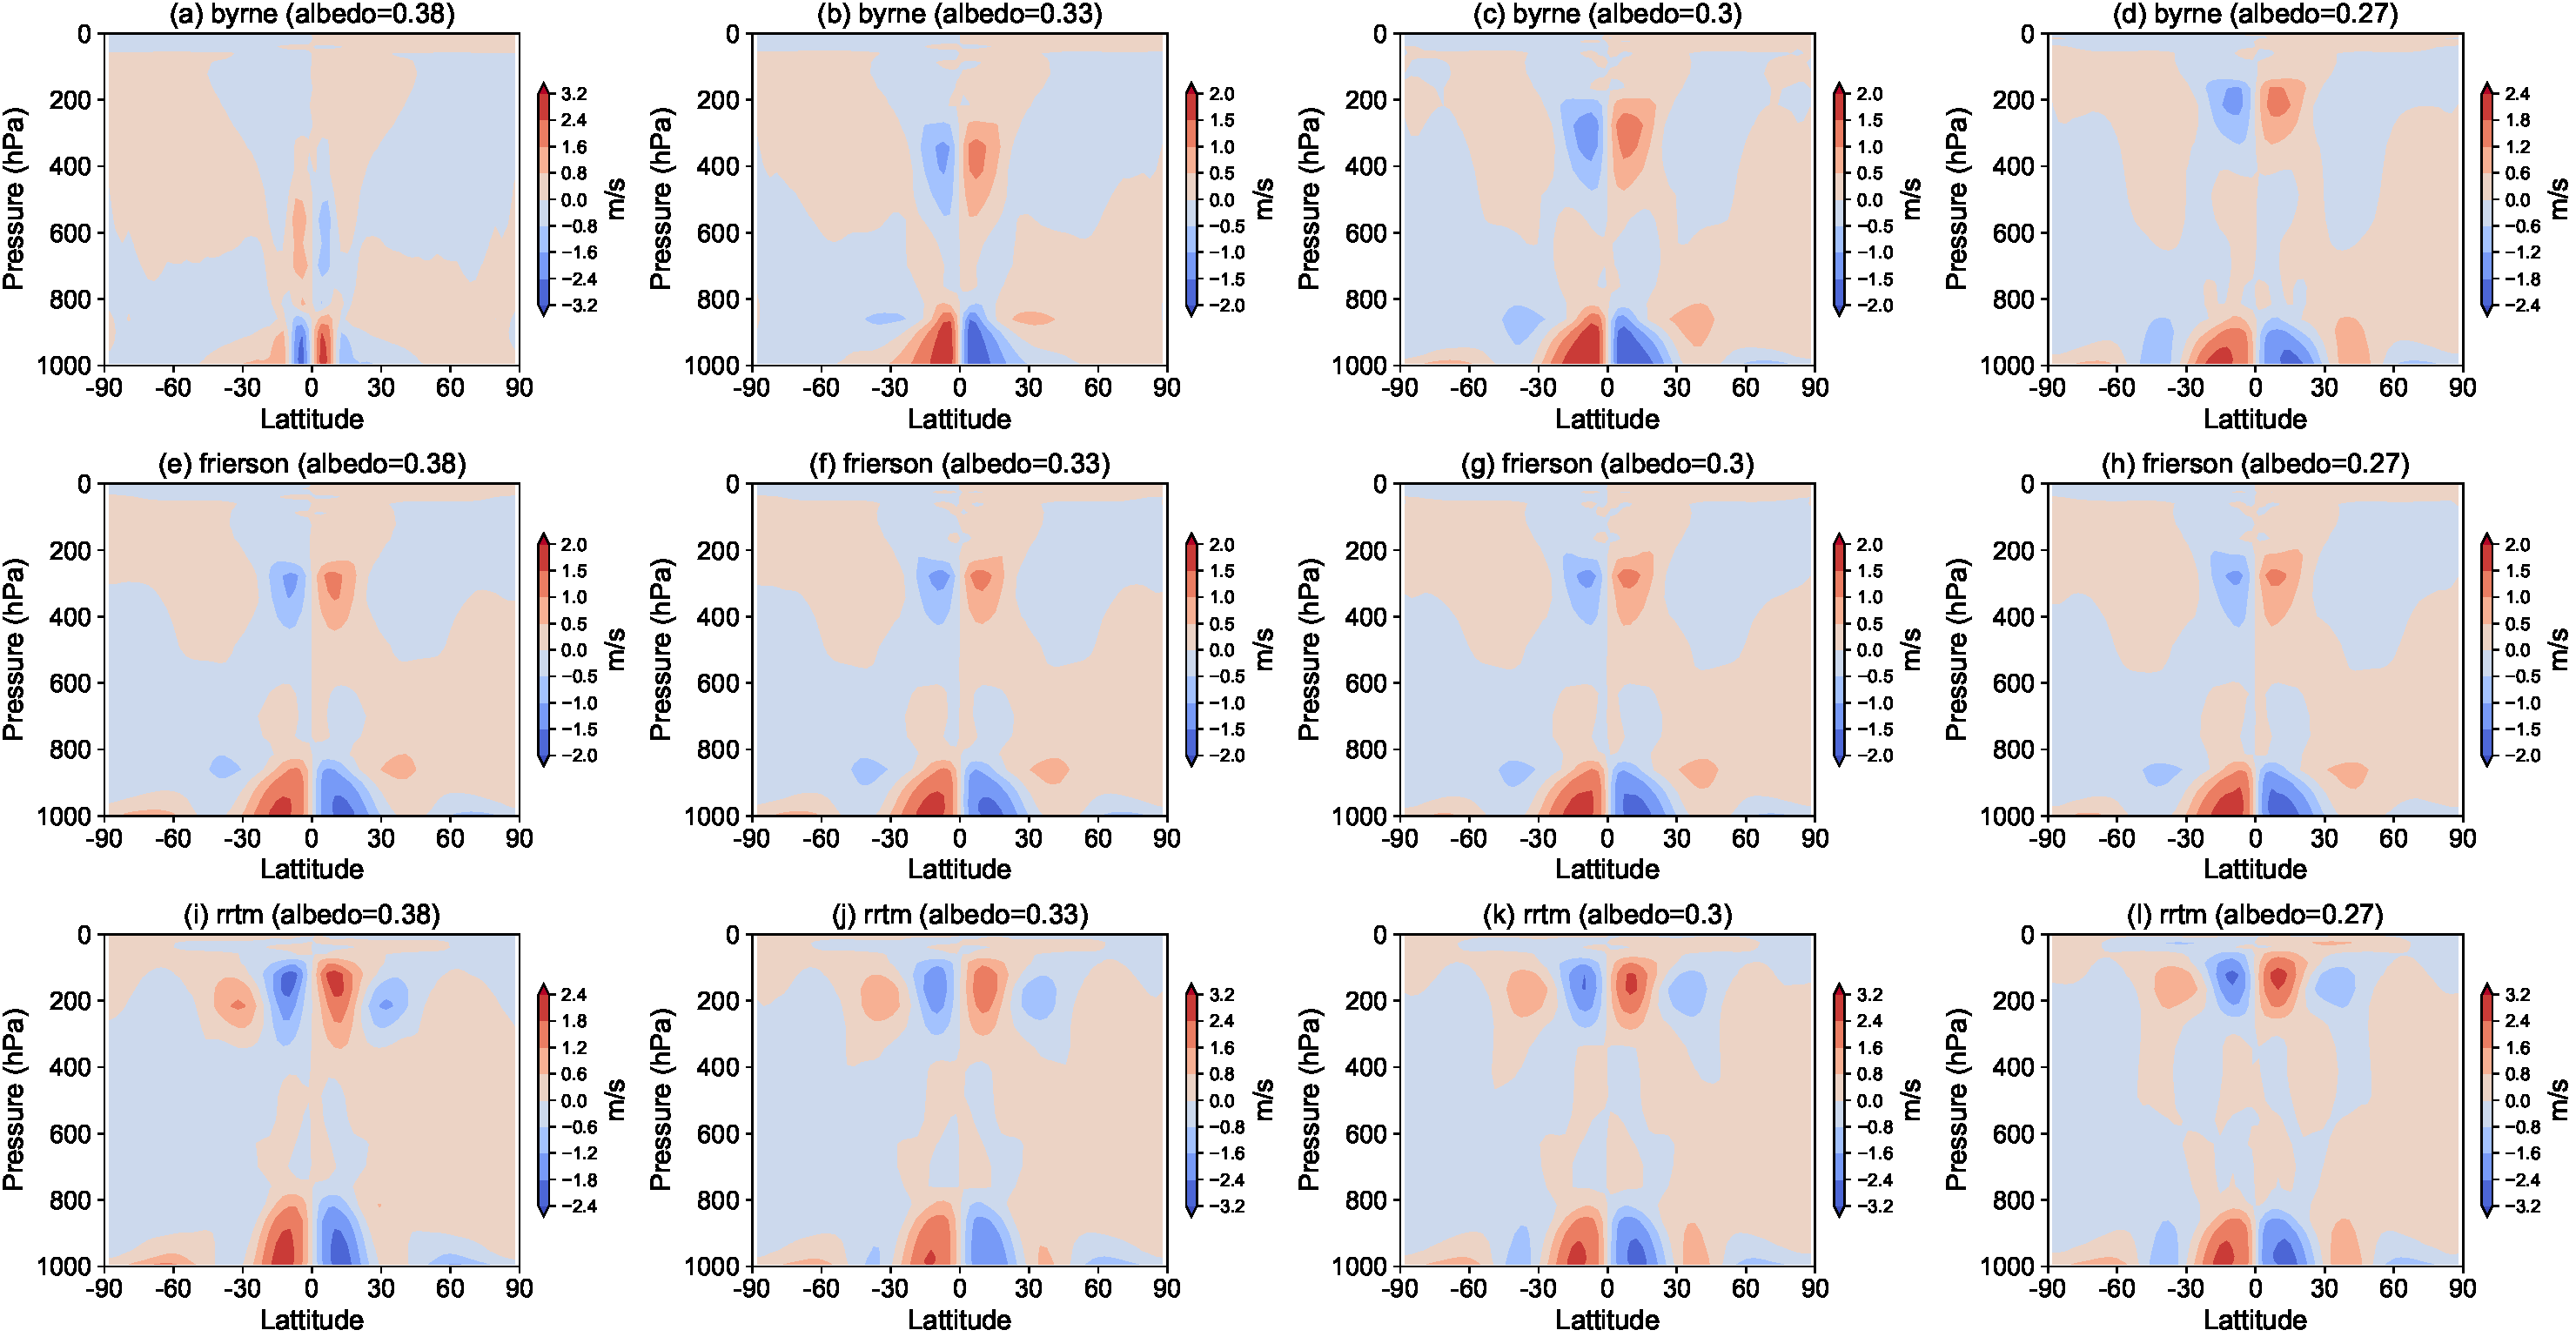
\includegraphics[width=1.0\linewidth]{{figs/polar_amp/fig_three_rad_scheme_coolwarm_4_albedos/vcomp_vert_profile_all_three_albedos}.pdf}
%	\caption{Annual mean and zonally averaged meridional velocity vertical profiles for the experiments with different radiation schemes and albedos.}
%	\label{fig:v_zonal}
%\end{figure}

%In summary, the change of latent heat transport with different albedos may be related to the zonal mean surface temperature change so as to polar amplification. What's more, the reversal of meridional velocity and the ensuing reversals of Hadley cell circulation and latent heat transport give an explanation for the abnormal behaviours of the experiment with albedo is 0.38 in the BOG radiation scheme.


%\subsection{Effect of climate feedbacks}
\subsection{Decomposition of surface temperature response}
\label{sec:climate_feedbacks_temp_decomp}

%\subsubsection{Decomposition of surface temperature response}

In \secref{sec:method_radiative_kernel}, with the aid of the radiative kernel method, we have obtained the zonal mean radiative feedback parameters for the BOG, Frierson and RRTM radiation schemes in the Isca model (\figref{fig:all_feedbacks}), which enables us to investigate the relative importance of each feedback to zonal mean surface temperature change. Following \cite{Feldl2013} and \cite{Kim2018}, we decompose the surface temperature change into various components after rearranging the \Eqref{eq:delta_R_relation}:

% we have decomposed the climate feedbacks into Planck feedback, lapse rate feedback, water vapor feedback but without cloud feedback, which is different from 

\begin{equation}
	\Delta T_s = \frac{1}{\overline{\lambda_P}}\left[\Delta R -\left(\lambda'_P+\sum_{i}\lambda_{NP_i}\right)\Delta T_s-\Delta F\right],
	\label{eq:decomp_Ts}
\end{equation}
where $\overline{\lambda_P}$ designates the global mean Planck feedback, by which all the feedbacks will be normalized, including the local deviation of the Planck feedback ($\lambda'_P$) from its global mean and all the other non-Planck feedbacks ($\lambda_{NP_i}$). As mentioned earlier, the cloud feedback and albedo feedback are not included in the experiments and thus lapse rate and water vapor feedback are the only two non-Planck feedbacks in \Eqref{eq:decomp_Ts}. $\Delta R$ is the net TOA radiative flux and it should be equal to the change in the convergence of horizontal atmospheric heat flux, referred to as the heat transport term. $\Delta F$ is the forcing after changing albedos estimated by fixed-SST method.


The contributions to the zonal mean surface temperature change in the BOG, Frierson and RRTM radiation schemes are displayed in \figref{fig:delta_ts_decomp}. We first look at the results from the RRTM radiation scheme as it provides a more realistic radiation scheme. As shown in \figsref{fig:delta_ts_decomp}g-i, the sum of the different components (red thick dash-dotted line) reproduces the actual surface temperature change (blue thick solid line) in the RRTM scheme either in the cooling (\figsref{fig:delta_ts_decomp}g, h) or warming (\figref{fig:delta_ts_decomp}i) cases, which implies we can analyze the relative importance of various components. As analyzed by \cite{Pithan2014}, the Planck feedback itself will automatically cause greater temperature change in high latitudes. In fact, according to the Stefan-Boltzmann law, the longwave radiation emitted by the Earth's surface ($R_s$) is
\begin{equation}
	R_s = \epsilon\sigma T^4,
\end{equation}
where $\epsilon$ is surface emissivity, which is close to 1, and $\sigma$ the Stefan-Boltzmann constant with value of $5.67\times 10^{-8}$ Wm$^{-2}$K$^{-4}$. Assuming there is a uniform radiation disturbance ($\Delta R$) at TOA, the surface temperature has to change by $\Delta T$ to balance $\Delta R$, and $\Delta T$ given by

\begin{equation}
\Delta T =\frac{\Delta R_s}{4\epsilon\sigma T^3}=\frac{\Delta R}{4\epsilon\sigma T^3},
\end{equation}
in which $\Delta R_s$ is the radiation change at the surface. It is clear that the temperature response ($\Delta T$) is large when the temperature ($T$) is low (e.g. polar region) and $\Delta T$ is small when T is relative high (e.g. tropical region). Therefore, the temperature response from Planck feedbacks (orange lines in \figsref{fig:delta_ts_decomp}g-i) is large at high latitudes and small at low latitudes. It should be pointed out that the Planck feedback is a negative feedback, but here \figref{fig:delta_ts_decomp} shows the local deviation of the Planck feedback from its global mean value and that is why the temperature response is negative in \figsref{fig:delta_ts_decomp}g, h, and positive in \figref{fig:delta_ts_decomp}i. For the temperature response caused by lapse rate feedback (green solid lines in \figsref{fig:delta_ts_decomp}g-i), it is positive in the polar region and negative in tropical region in the warming case and the signs are opposite in the cooling case, indicating that the lapse rate feedback will amplify the temperature response in high latitudes. The positive lapse rate feedback in the polar region is due to the bottom-heavy warming/cooling vertical structure (\figref{fig:vert_temp_diff}). Our finding in the warming case is consistent with the result under equinox insolation in \cite{Kim2018}, but they show that things are different under seasonal and annual mean insolation conditions in which the lapse rate feedback is globally negative \citep[see Fig. S1 of][]{Kim2018}. This is because the induced temperature change is not enough to form an inversion layer near the surface \citep{Kim2018}. %\figref{fig:kim2018_lapserate}

% different from the results of \cite{Kim2018}, where the lapse rate feedback is globally negative under seasonal insolation.

%The stable atmospheric structure in the polar region making the lapse rate feedback positive

\begin{figure}[ht]
	\centering
	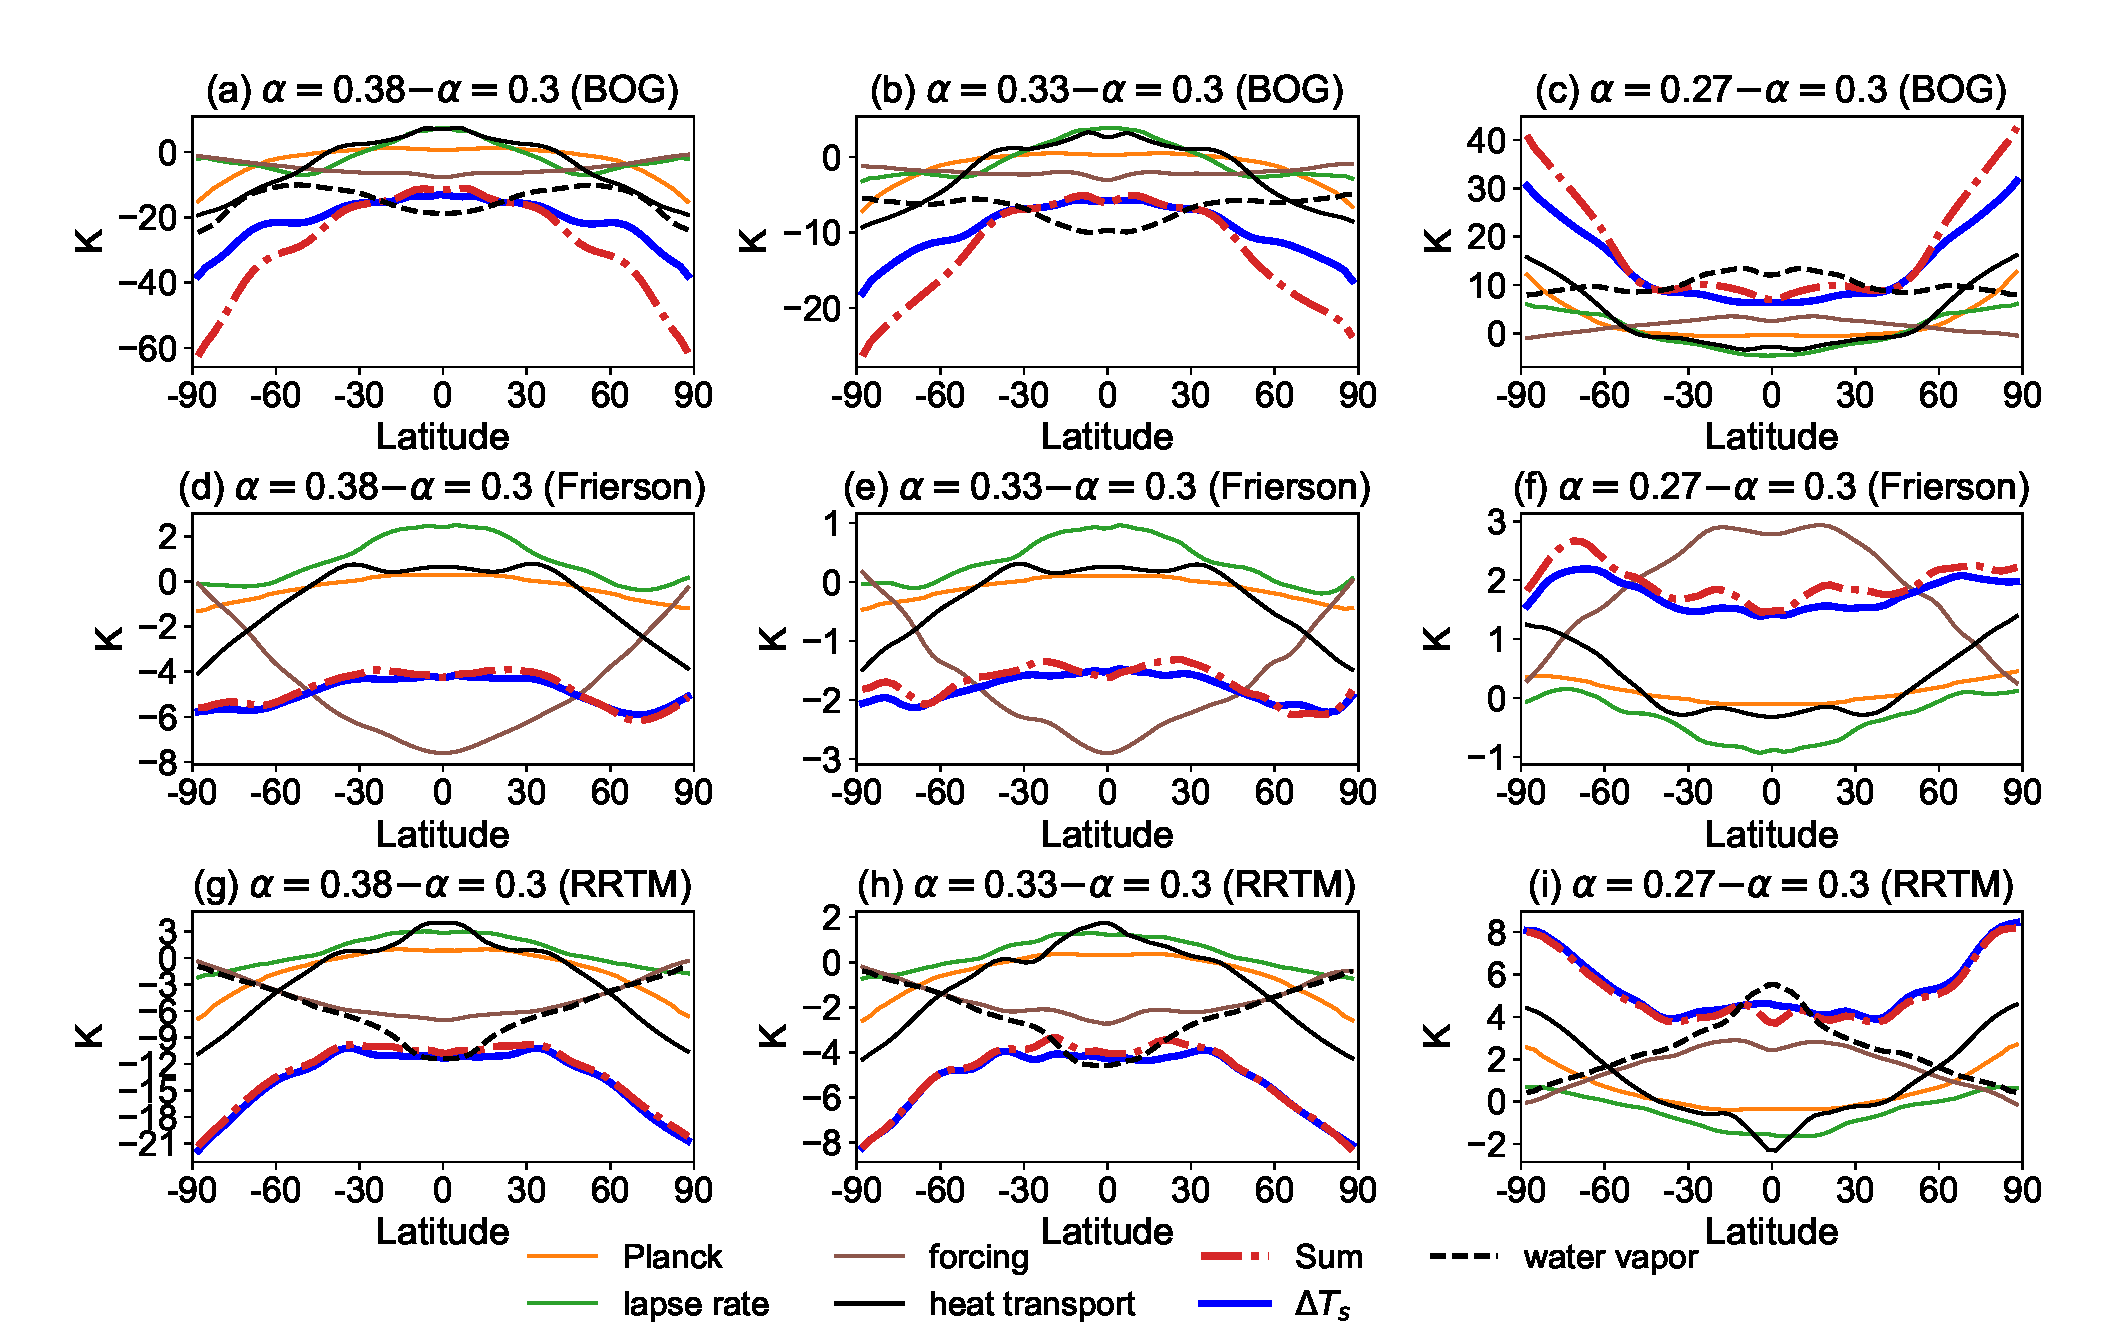
\includegraphics[width=1.0\linewidth]{figs/polar_amp/delta_ts_decomp}
	%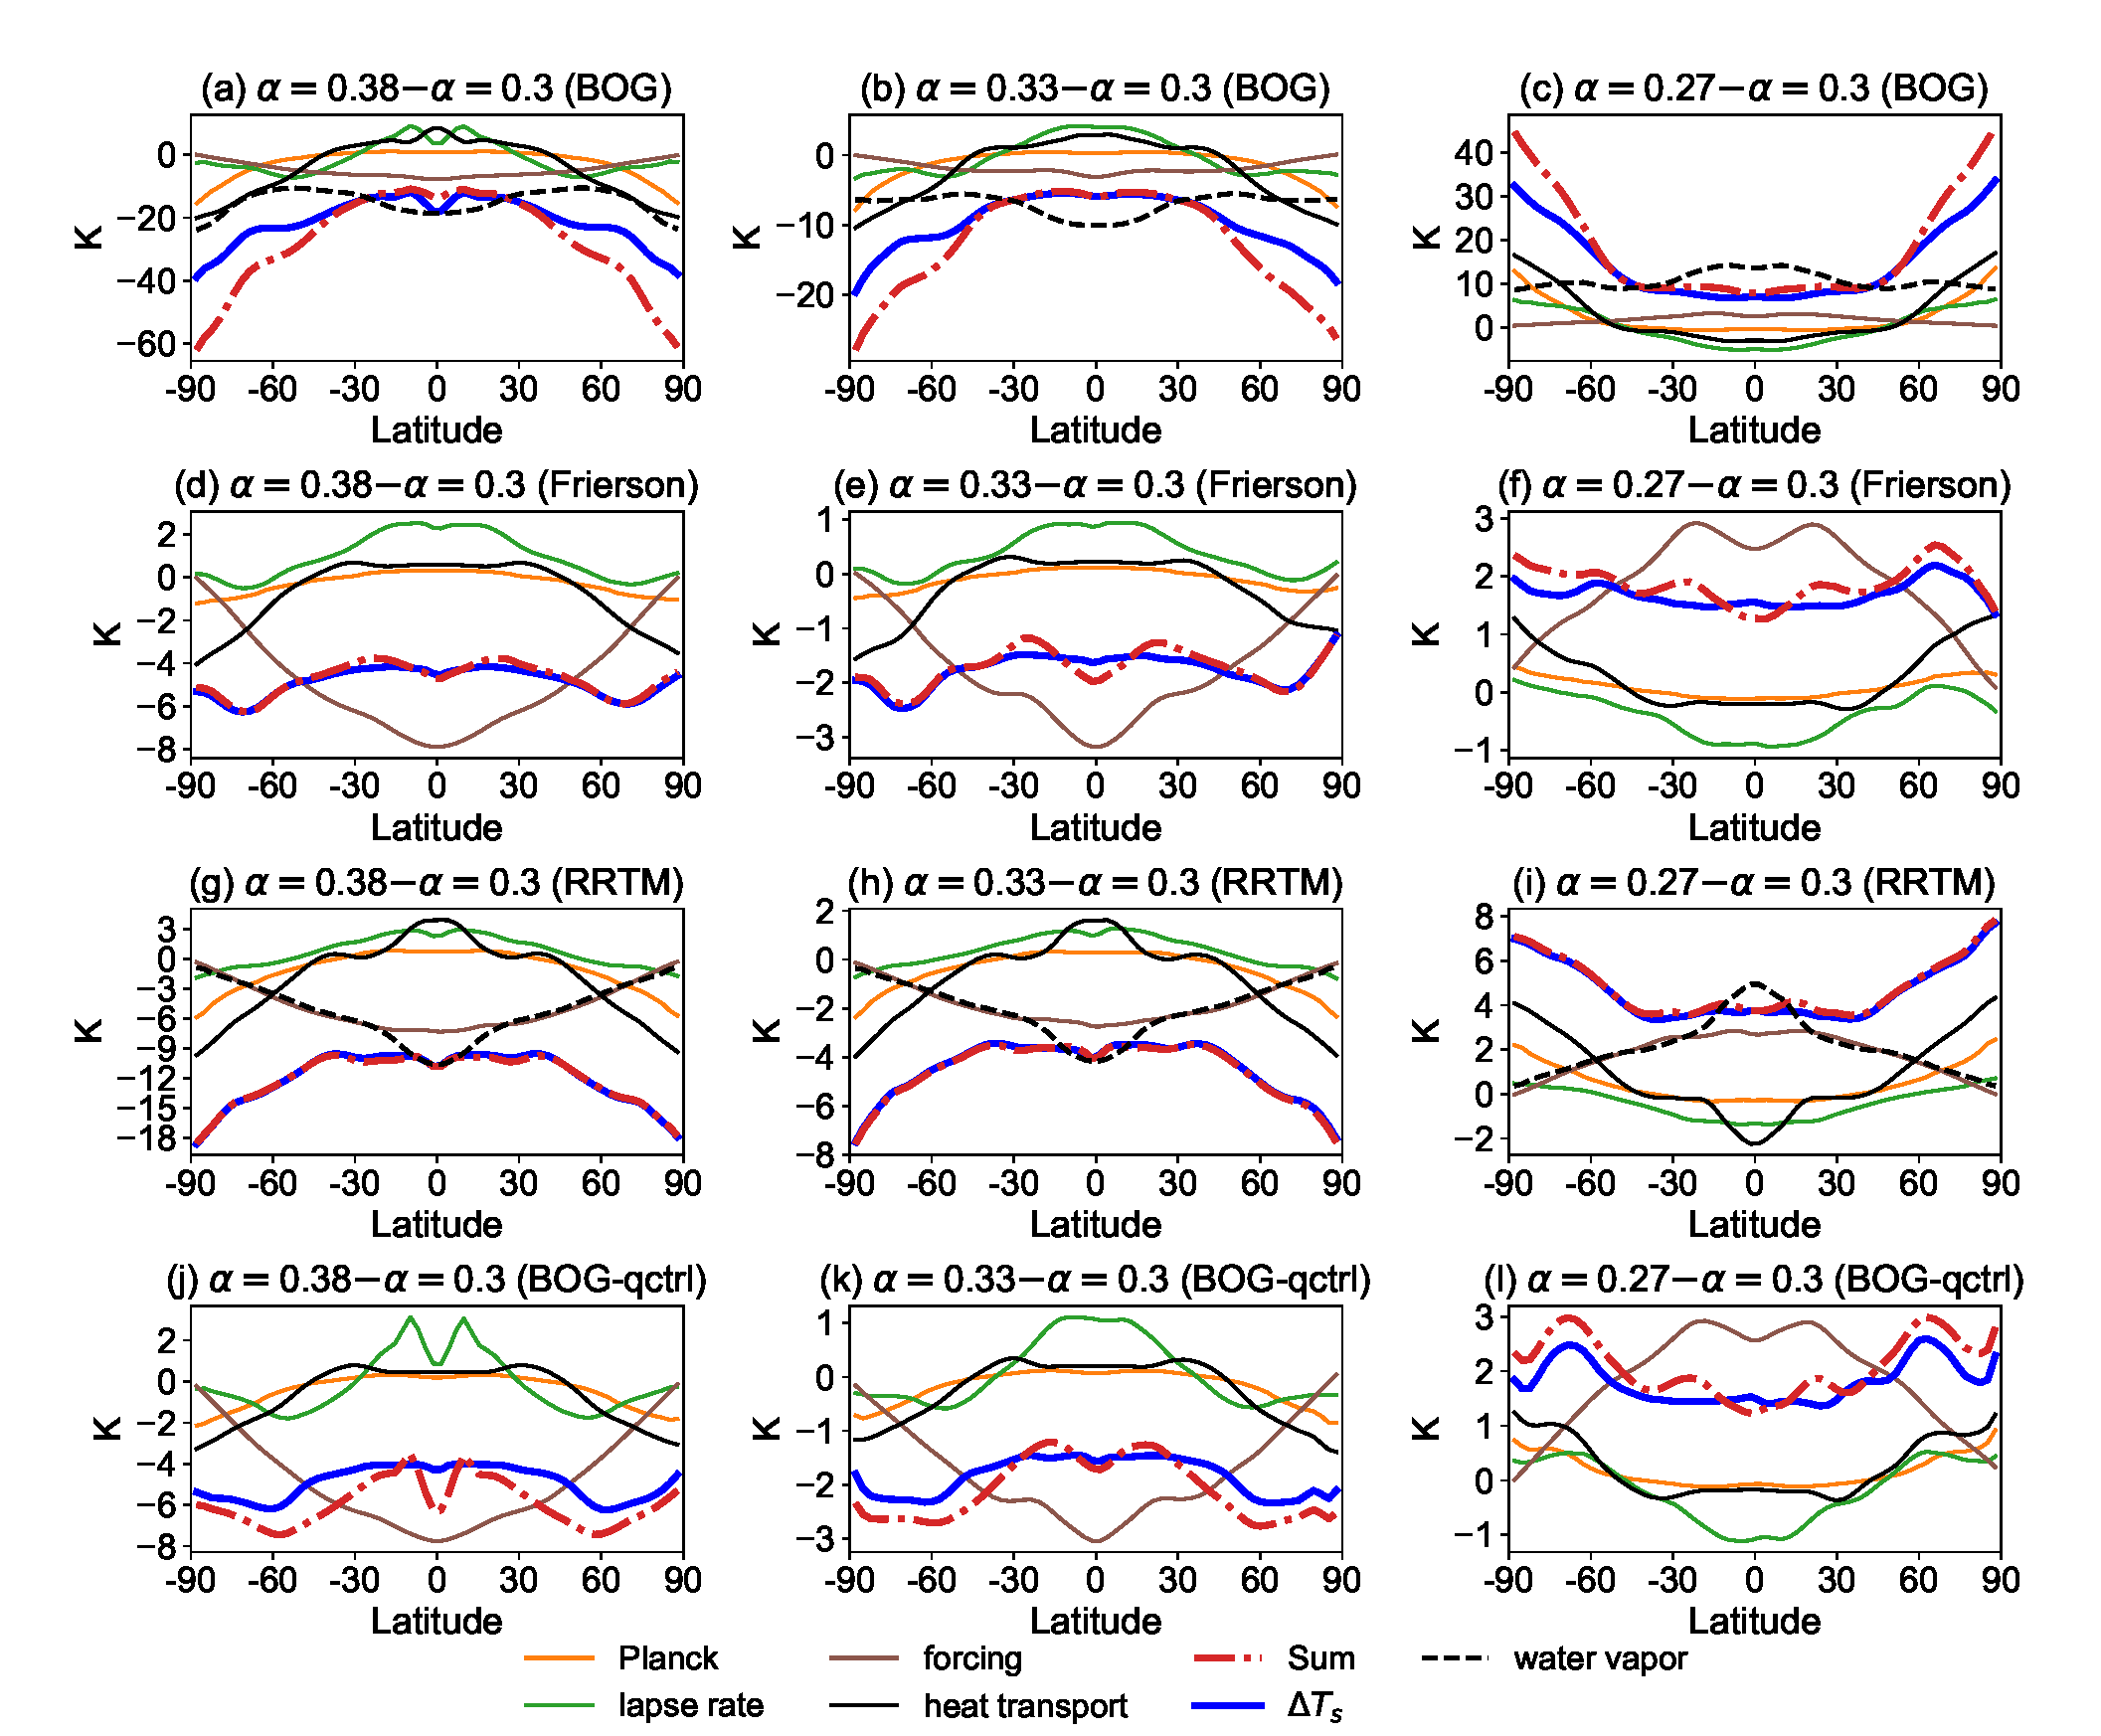
\includegraphics[width=1.0\linewidth]{figs/polar_amp/delta_ts_decomp_q.pdf}
	\caption[Zonal and annual mean contributions of surface temperature changes from forcing, heat transport and climate feedbacks]{Zonal and annual mean contributions of surface temperature changes for (a)-(c) BOG scheme, (d)-(f) Frierson scheme, (g)-(i) RRTM schemes and (j)-(l) BOG scheme without moisture feedback respectively. The components include Planck feedback (orange), lapse rate feedback (green), forcing (brown), water vapor feedback (black dashed) and heat transport (black solid), all of which are weighted by global and annual mean of the Planck feedback following \cite{Feldl2013a} and \cite{Kim2018}. The sum of the different components is shown in thick red dash-dotted lines and the surface temperature change in the experiments is indicated by thick blue lines. The first, second and third columns are for experiments when albedo is changed from 0.3 to 0.38, 0.33 and 0.27 respectively.}
	\label{fig:delta_ts_decomp} 
\end{figure}

% \begin{figure}[ht] %
% 	\centering
% 	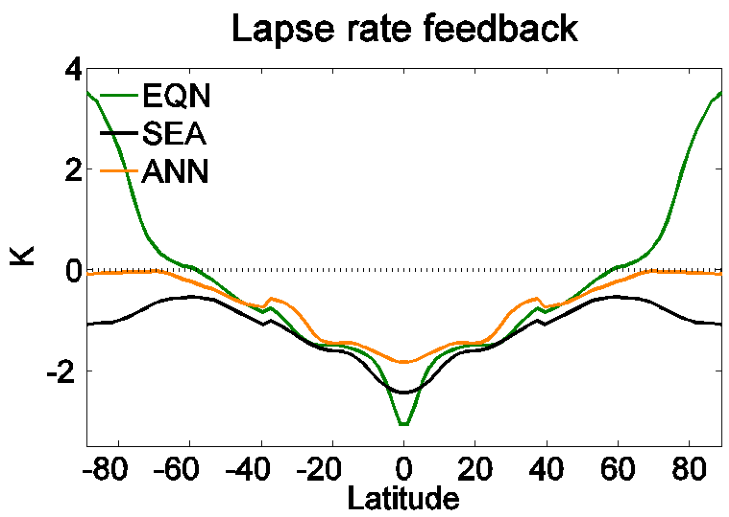
\includegraphics[width=.6\linewidth]{figs/polar_amp/Kim2018_lapserate}
% 	\caption{Zonal- and time-mean partial temperature changes (K) attributed to lapse rate feedback in GFDL AM2 under equinox (EQN, green), seasonal (SEA, black), and annual mean (ANN, orange) insolation. Adapted from Figure S1 of \cite{Kim2018}.}
% 	\label{fig:kim2018_lapserate}
% \end{figure}

The heat transport contributes most to the surface temperature change in the polar region both in the cooling and warming cases in our study, but it is different from the calculation of \cite{Pithan2014}, where they find that the temperature related feedbacks contribute most to the Arctic warming when there is a surface albedo feedback. When there is a lack of surface albedo feedback, the heat transport is also the largest contributor to polar amplification under seasonal solar radiation according to \cite{Kim2018}. In the warming case (\figref{fig:delta_ts_decomp}i), the heat transport cools the low latitudes and warms the high latitudes, which decreases the large meridional temperature and energy imbalance gradients. As illustrated in \figsref{fig:delta_ts_decomp}g-i, the water vapor feedbacks contribute more to the tropical warming or cooling rather than to polar regions, which is consistent with the conclusion of \cite{Pithan2014}. But water vapor does have an effect on the temperature change due to the enlarged climate sensitivity \citep{Langen2012}. In fact, the temperature responses due to water vapor feedbacks in the BOG scheme (black dashed lines in \figsref{fig:delta_ts_decomp}a-c) are different from that in the RRTM schemes. They do not tend to zero as latitude increases. Instead, they are relative flat at high latitudes, which could possibly be used to explain the abnormal surface temperature response in the BOG scheme. Regarding the forcing (brown lines in \figsref{fig:delta_ts_decomp}g-i) due to the change of albedos, it is larger in low latitudes than in high latitudes as the solar radiation is strong at low latitudes, and hence it will amplify the temperature change at low latitudes.

 \begin{figure}[ht]
    \centering
	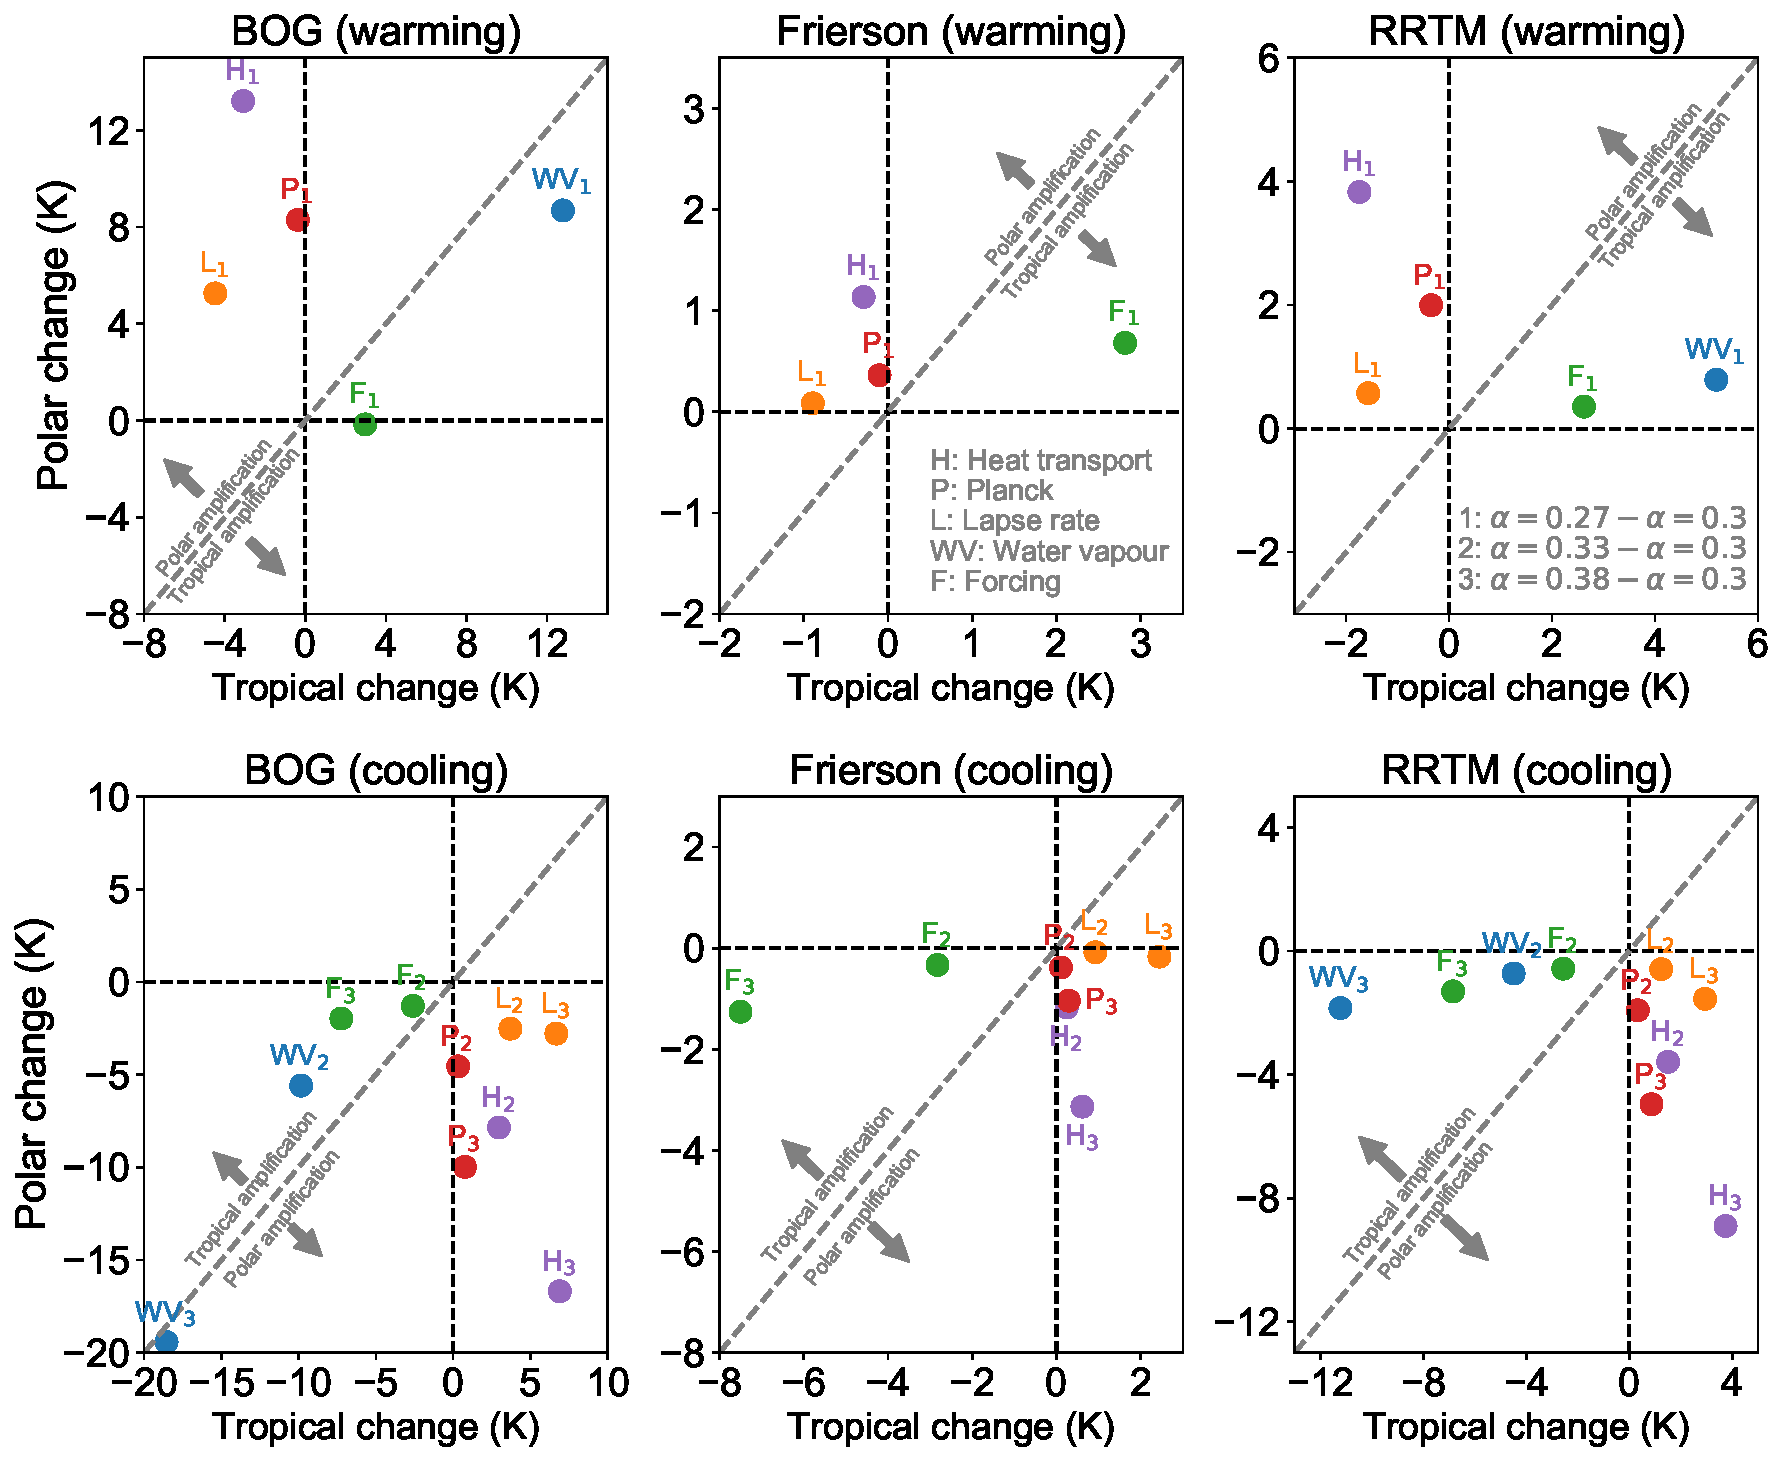
\includegraphics[width=0.9\textwidth]{figs/polar_amp/contributions_to_polar_amplification.pdf}
	\caption[The contributions of various factors to polar versus tropical temperature changes from a TOA perspective]{The contributions of various factors to polar versus tropical temperature changes from a TOA perspective. The factors are shown in the legend, and those above the 1:1 line contribute to polar amplification, whereas feedbacks below the line oppose polar amplification. The upper and bottom panels are for the warming (subscript 1) and cooling (subscripts 2 and 3) cases respectively. The titles of each figure indicate the radiation schemes used in the runs.}
	\label{fig:contribution_pole_vs_tropic}
\end{figure}

The roles of lapse rate feedback, Planck feedback and heat transport in the BOG (\figsref{fig:delta_ts_decomp}a-c) and Frierson (\figsref{fig:delta_ts_decomp}d-f) schemes are similar to those in the RRTM scheme, except the role of water vapor feedback in the BOG scheme, which is much larger at high latitudes compared to others. One strange thing is the sum of these contributions is greater than the actual temperature response at high latitude in the BOG scheme, for which a possible reason is that the decomposition of the surface temperature change is linear and some non-linear factors may have an influence at high latitudes. We can see that after the water vapor feedback is disabled in the BOG scheme, the sum of these various components is close to $\Delta T_s$ (\figsref{fig:delta_ts_decomp}j-l), indicating that the non-linear effect is possibly associated with water vapor. 

%\begin{figure}[ht] %[ht]
%	\centering
%	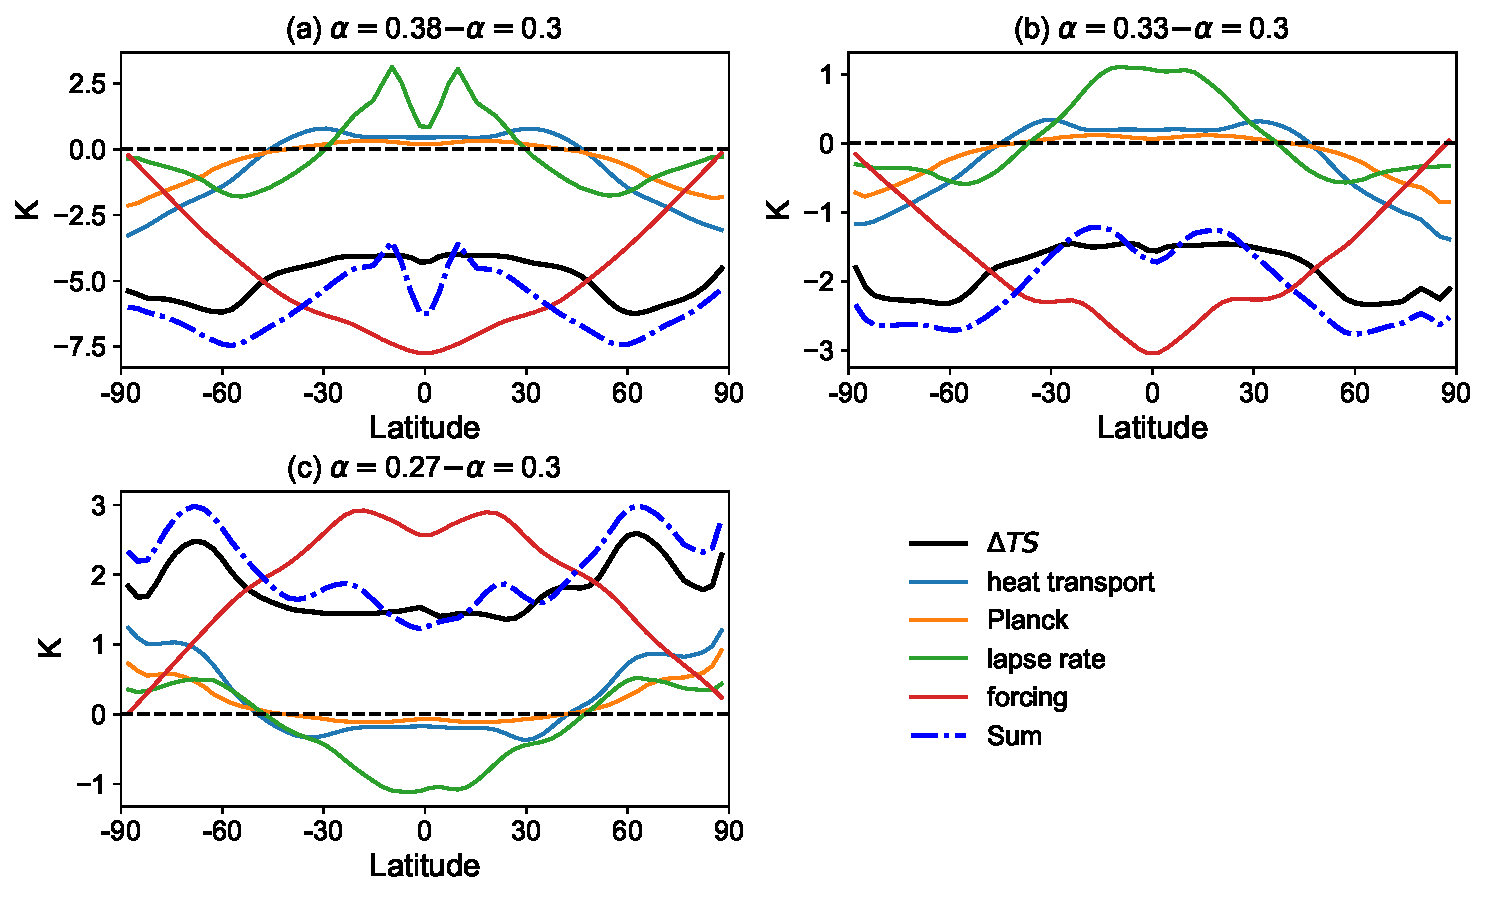
\includegraphics[width=0.8\linewidth]{figs/polar_amp/ts_decomp/delta_ts_decomp_fixed_q_byrne}
%	\caption{Zonal and annual mean contributions of surface temperature changes for (a)-(c) BOG radiation scheme without moisture feedbacks.}
%	\label{fig:delta_ts_decomp_bog_no_q_fb}
%\end{figure}

\section{Discussion and summary}
\label{sec:polar_amplification_summary}

In this chapter, we employ the Isca model to study the surface temperature changes in aquaplanet simulations with various radiation schemes and albedos in order to quantify the different mechanisms that could lead to polar amplification under equinox insolation. Two gray radiation schemes, BOG and Frierson, and one full radiation scheme, RRTM, are used in the simulations. The BOG scheme shows the largest surface temperature change and polar amplification, while the Frierson scheme shows the weakest surface temperature change when changing albedos. %, which is a way to disturb the radiation balance at TOA.

\begin{figure}[ht]
    \centering
	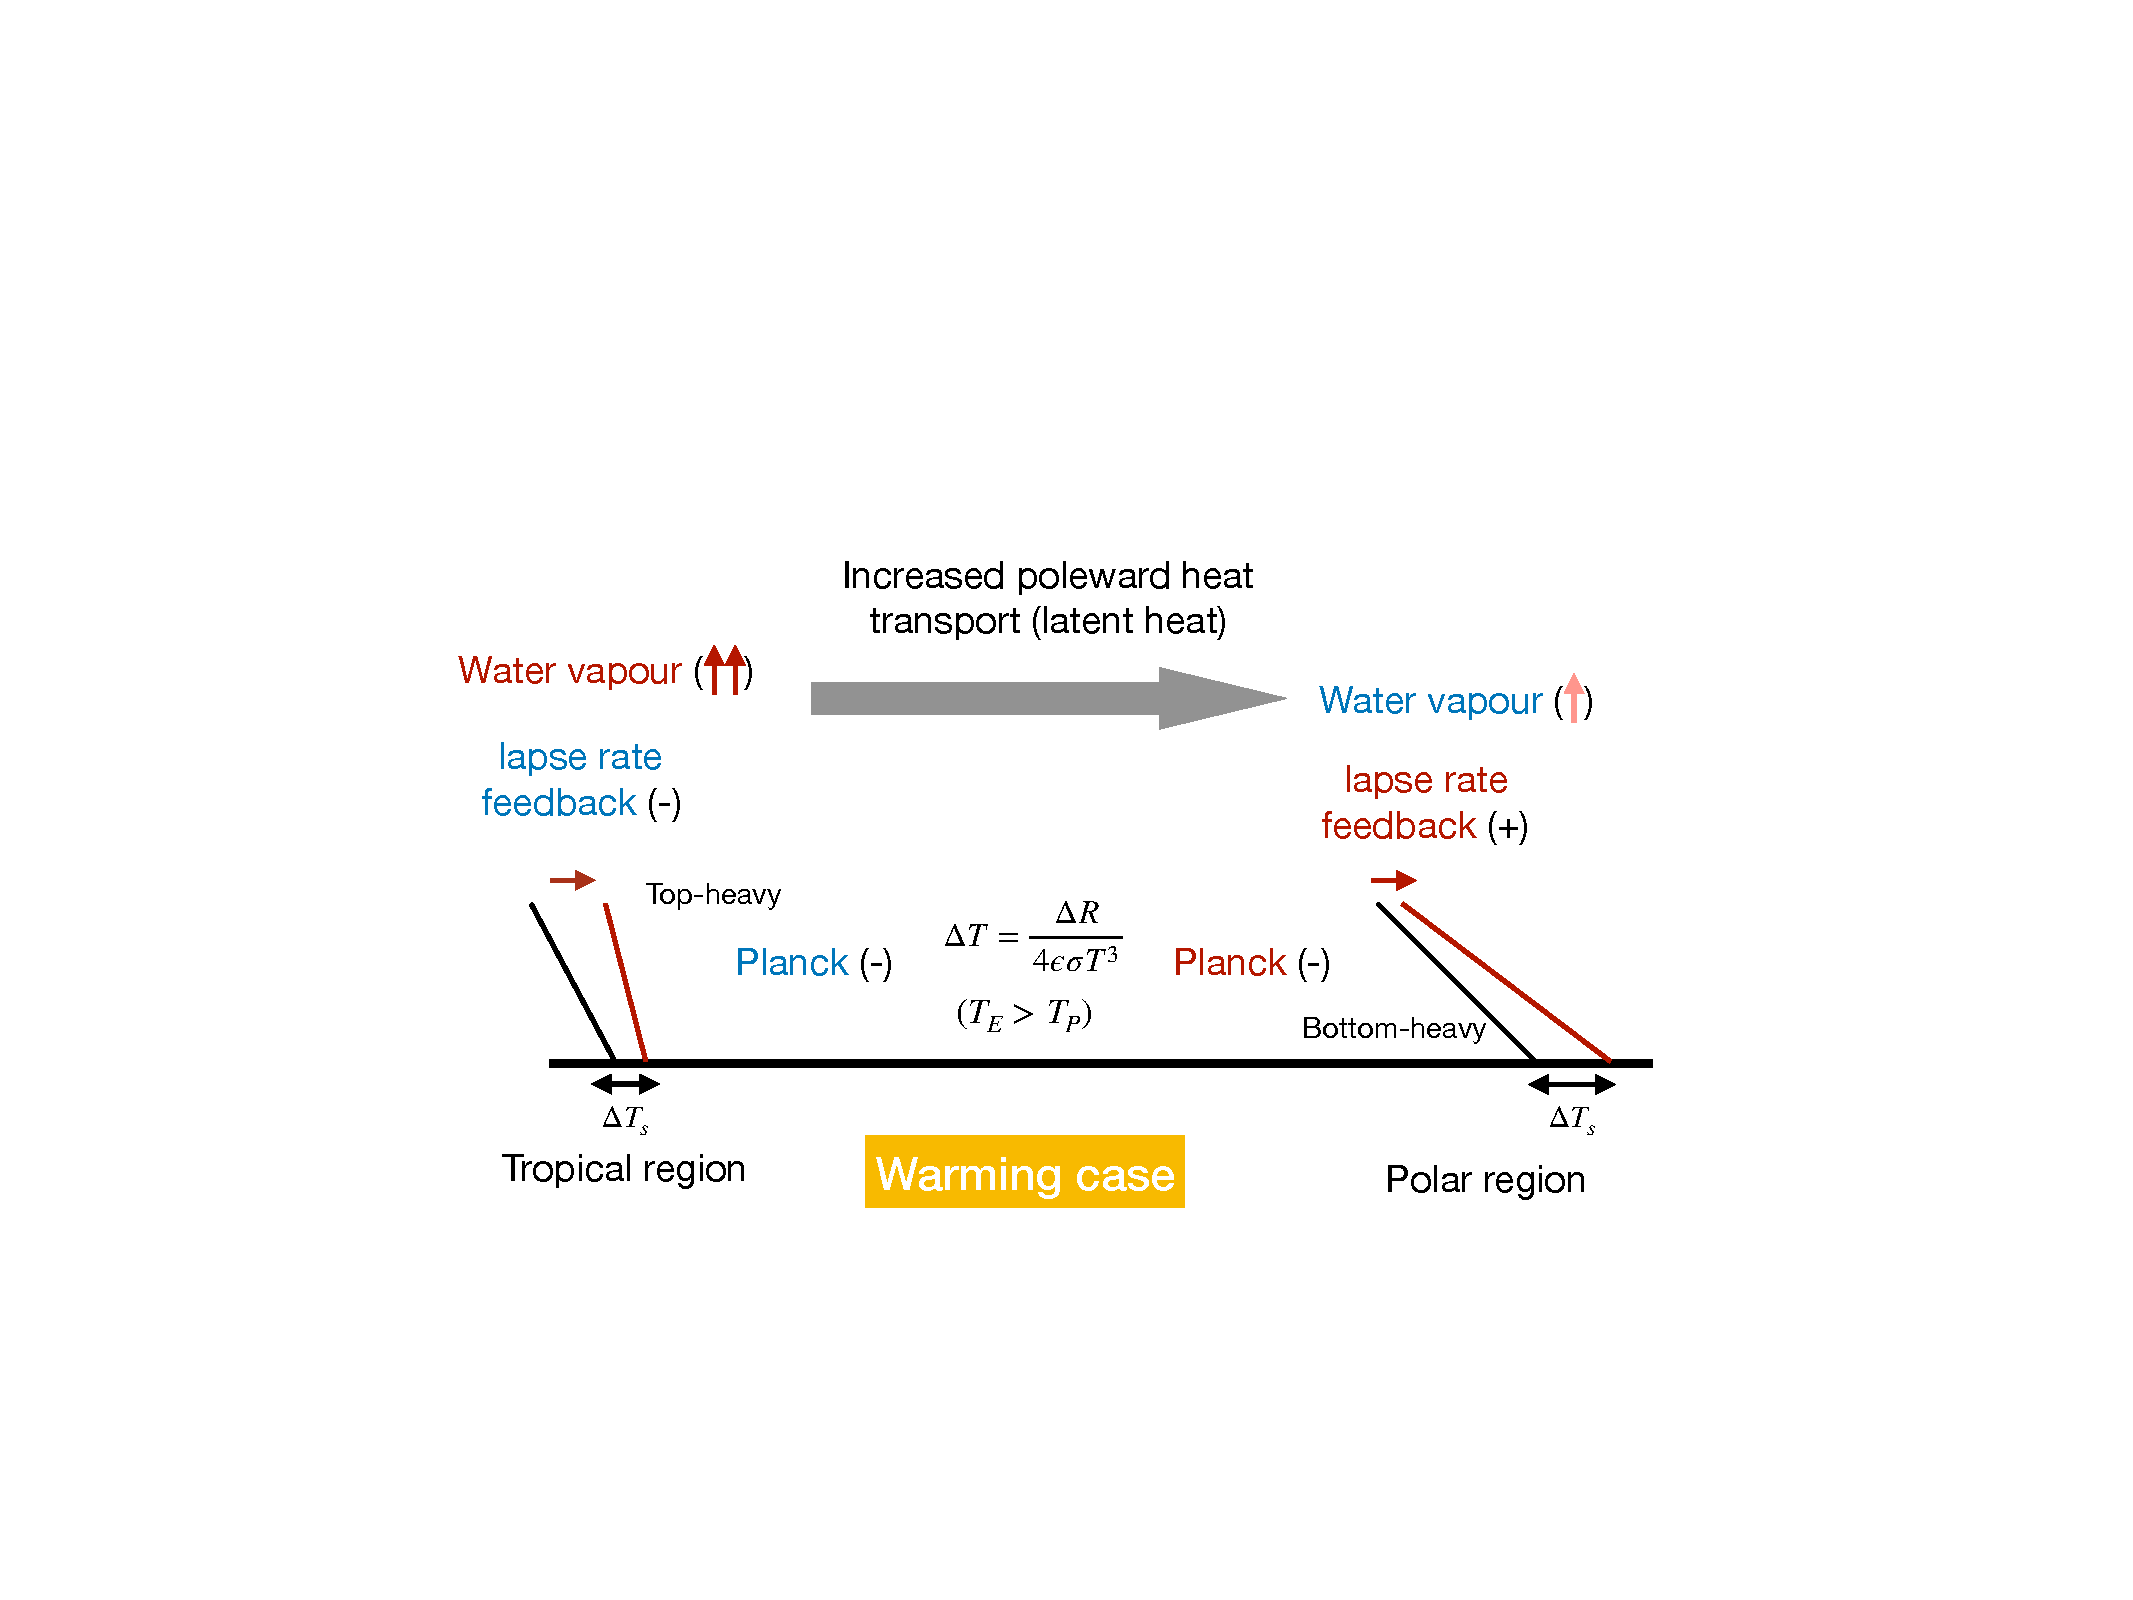
\includegraphics[width=0.8\textwidth]{figs/polar_amp/pa_dynamic.pdf}
	\caption{A schematic diagram to illustrate the various factors that contribute to polar amplification.}
	\label{fig:pa_mechanism_schematic}
\end{figure}

To examine why the temperature responses in the three radiation schemes (Frierson, BOG and RRTM) of Isca are different, the climate feedback processes within these three radiation schemes are analyzed. The feedbacks for each radiation scheme of Isca are computed from the radiative method \citep{Soden2008,Shell2008}, with the kernels derived from the offline calculation of the radiative transfer codes. The radiative kernels can be used among different simulations, which provides a solid basis for the feedback analysis.

The comparison of results from BOG and Frierson gives us some insights about the role of water vapor feedback in surface temperature change. After turning off the water vapor feedback in the BOG scheme, the surface temperature responses are much smaller and become close to the simulation results from the Frierson scheme. However, there is still the amplified surface temperature change at high latitudes, which is associated with the poleward atmospheric energy transport. Following \cite{Feldl2013} and \cite{Kim2018}, the decomposition of the surface temperature change illustrates the relative importance of various contributions to surface temperature change at high latitudes. Specifically, heat transport, Planck feedback and the positive lapse rate feedback at polar region are all supportive to polar amplification. However, water vapor feedback and the forcing induced by altering albedo contribute more to the surface temperature change at low latitudes than at high latitudes (\figref{fig:contribution_pole_vs_tropic}). In spite of that, the water vapor feedback is very strong at high latitudes in the BOG scheme, which could explain the large temperature response in the experiments. A schematic of the mechanisms that contribute to polar temperature changes is illustrated in \figref{fig:pa_mechanism_schematic}, which uses the warming case as an example. Due to the nonlinearity of the Planck feedback, the temperature change in response to the same radiative imbalance at TOA is larger in polar regions than in the tropical region, as the mean temperature is lower at high latitudes ($T_P<T_E$). That is to say, the Planck feedback supports polar amplification naturally. In addition, as illustrated in \figref{fig:pa_mechanism_schematic}, the polar region exhibits a bottom-heavy warming profile because of the stability at the lower troposphere, leading to a positive lapse rate feedback and less infrared radiation to be emitted to space. In contrast, deep convection is active in the tropical region, releasing more latent heat in the upper troposphere and thus favoring a top-heavy warming profile. Such a top-heavy profile brings a negative lapse rate feedback at low latitudes, which is more efficient at emitting the longwave radiation to space. Therefore, lapse rate feedback is favorable to polar amplification as well. However, the water vapor increases more in tropical regions than over polar regions in the warming case, and thus this positive feedback favors tropical warming.

In summary, our findings have confirmed that polar amplification could exist even without sea ice and surface albedo feedback in aquaplanet simulations, which is consistent with previous results \citep{Langen2007,Kim2018,Alexeev2005}. However, we have not explored the role of surface albedo feedback and cloud feedback in polar amplification, due to lack of sea ice and cloud schemes in the Isca model currently.

% As assessed by \cite{Kim2018}, the cloud radiative effects are negative in high latitudes due to an increase of low-level cloud amount and positive in low latitudes due to a decrease of overall cloud amount, which could explain in part why the polar amplification of surface temperature is large in our simulations. 

% But this will be studied in further chapters.

%Some studies also analyzed the effect of clouds radiative feedback to polar amplification \citep[e.g.][]{Kim2018}, where they found that polar clouds will have a cooling effect under global warming. Which could be

% \chapter{The Simple Diagnostic Cloud Scheme}

\section{Overview}

In order to have a cloud scheme that interacts with the radiation, we need to predict not only the cloud amount but also its radiative properties. We focus mainly on the former, for the latter we require effective radius of the cloud droplets, and in-cloud liquid water content. In the following subsections we describe how these are specified; an encapsulation of the cloud scheme is also given in \figref{fig:cld_scheme_summary}. 

\begin{figure}[t]
	\centering
	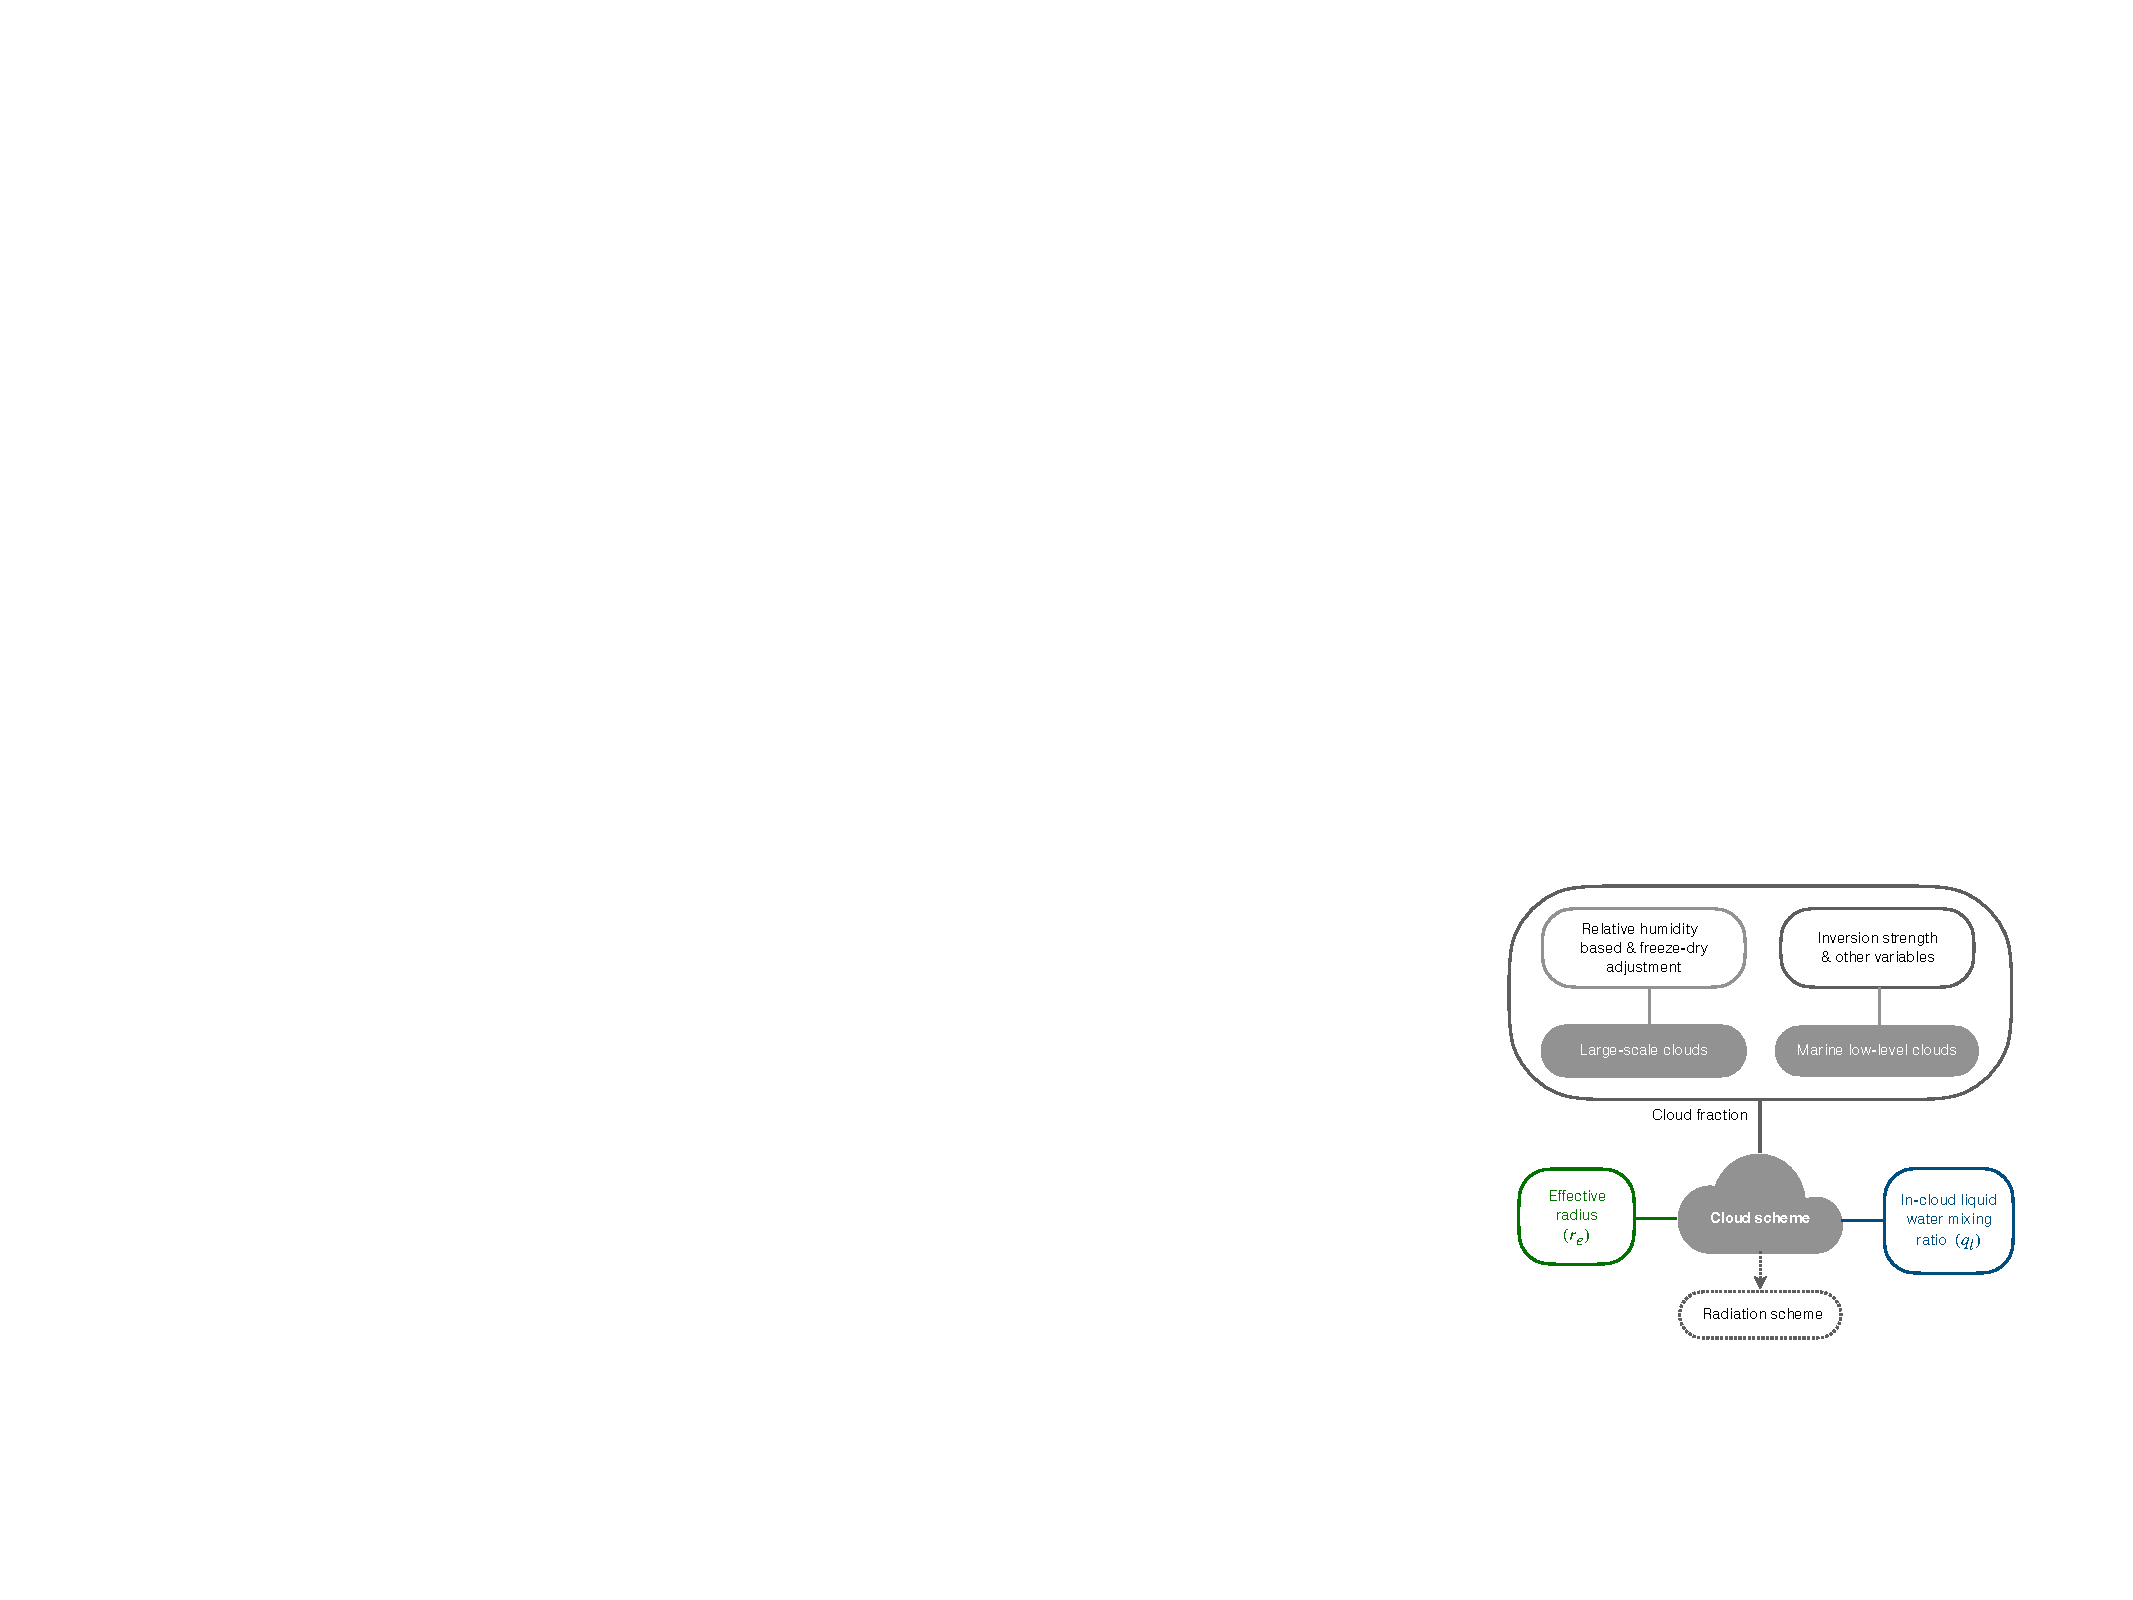
\includegraphics[width=0.7\linewidth]{figs/simple_cld_scheme/diag_cld_scheme_summary.pdf}
	\caption{A sketch of the simple cloud scheme components, which include the cloud fraction, effective radius of cloud droplet and in-cloud liquid water mixing ratio. At any given location, the maximum of the cloud fractions from large-scale cloud scheme and marine low stratocumulus cloud scheme is applied if both of them are used.} 
	\label{fig:cld_scheme_summary}
\end{figure}

%Clouds are represented in two ways in the scheme, `large-scale' clouds and low clouds. 
As noted in the introduction, large-scale clouds are parameterized as a function of relative humidity and this provides the majority of the cloud cover. However, as discussed in XXXXXXXXXXXXXXXXXX, this scheme alone is found to be inadequate and two additional effects are needed. First, a `freeze-dry' method based on the specific humidity is used to reduce the large-scale cloud cover over polar regions to more realistic levels. Second, a separate marine low stratus cloud scheme is used to represent the stratiform clouds (which have a large shortwave radiative effect), and this has a particularly large effect in subtropical regions off the west coast of continents. These two additional components are optional and users can decide whether to use according to their research interest. Although these clouds have different physical properties (e.g., cloud top temperature), all of them are treated essentially as liquid clouds in our scheme. The effective radius of the cloud droplets is allowed to change with temperature, and this affects the radiative transfer. Some tuning of the clouds scheme is performed in order to fit the observations. Nevertheless, the values of certain parameters used in the scheme are not necessarily definitive and may be varied in order to examine the sensitivity of clouds to perturbations such as CO$_2$ increase. 

The present version does not include a separate scheme for convective clouds, and the convection scheme in the model has no effect on cloudiness except in so far as it may change the relative humidity or, possibly, the low-level inversion.
%An alternative way to proceed would be to diagnose the convective clouds based on precipitation \citep[e.g.,][]{Gordon1992,Hack1998}, including that predicted by the convection scheme. 
We find that the vertical structure of clouds can be simulated relatively well without explicit diagnosis of convective clouds (see Figure..... \ref{fig:cld_fraction_profile}), and we leave the possible explicit representation of convective clouds to a future study. 


\section{Cloud fraction}

\subsection{Relative humidity-based cloud fraction}
\label{sec:rh_cloud}

The use of a relative humidity scheme is based on the notion that over a grid box the humidity varies, and that condensation will occur and clouds will form even when the grid cell is not saturated \citep{Tompkins2005, Quaas2012}, and one such scheme is that of \citet{Sundqvist1989}, discussed more below. Such schemes do not account for variations in dynamical conditions except in so far as they are reflected in the relative humidity field, but they form a simple rational basis for cloud prediction. Here we implement a large-scale cloud scheme in which the cloud fraction ($C_{s}$) is a piecewise linear function of grid-mean relative humidity ($H$), namely
\begin{equation}
	C_{s}=\min\left(1, ~\max \left(0, ~ a \cdot (H -1) + 1 \right)\right).
	\label{eq:linear_cf_rh} 
\end{equation}
The diagnosed cloud fraction is therefore unity when the mean relative humidity equal to one (i.e. grid-box is saturated). The value of $a$ determines the critical value of relative humidity, $H_c$, above which clouds form, so that $a=1/\left(1-H_{c}\right)$ and $H_c = (a -1)/a$. The coefficient $a$ (and hence $H_{c}$) is taken to be a function of height (or pressure) but not latitude or longitude.  We also have implemented the \citet{Sundqvist1989} scheme, and that is available for users, but we do not describe it here. 

We derive the coefficient profile, the vertical values of the coefficient $a$, of the linear relationship between $C_s$ and relative humidity based on reanalysis data sets. Specifically, the hourly relative humidity and cloud fraction data sets in year 2017 from the European Centre for Medium-Range Weather Forecasts (ECMWF) Reanalysis version 5 (ERA5) \citep{era5} are used to derive the coefficient profile. The ERA5 has $1^{\circ}\times 1^{\circ}$ horizontal resolution and 37 vertical levels. For each vertical level, the piecewise linear relationship (as cloud fraction is not allowed to be smaller than 0 or larger than 1) is used to fit the cloud fraction against relative humidity with a least squares method, then the coefficient $a$ of that level is obtained. In addition, data sets with three different horizontal resolutions, including $0.75^{\circ}\times 0.75^{\circ}$, $1.4^{\circ}\times 1.4^{\circ}$ (T85) and $2.8^{\circ}\times 2.8^{\circ}$ (T42), are used to test whether the derived coefficient profile is sensitive to horizontal resolution. The derived profiles with different resolutions are shown in \figref{fig:linear_coeff_profile}a, and the corresponding critical relative humidity ($H_c$) profiles are shown in \figref{fig:linear_coeff_profile}b for reference. At very high resolution we would expect the humidity distribution in a given grid box to be narrower, and hence the critical value of relative humidity to increase, however we find that the horizontal resolution has a relatively small influence on the coefficient profiles at the resolutions we consider here. 

To apply the coefficient profile of $a$ in the model, a profile similar to the Equation (3) from \citet{Quaas2012} is used: %In addition, the global and regional data are also used to check whether the coefficient profiles would be different in various regions.
\begin{equation}
	a = a_t + (a_s-a_t)\exp{\left[1-\left( \frac{p_s}{p} \right)^{n} \right]},
	\label{eq:linear_coeff_a}
\end{equation}
where $p$ is the pressure, $p_s$ is the surface pressure, $a_s$ and $a_t$ are the values of coefficient $a$ at surface and free troposphere respectively. Such a functional form fits the observations fairly well with only a small number of tunable parameters. We use $a_s=36$, $a_t=13$ and $n=12$, which determines shape of the profile. The fitted profile for $a$, as indicated by the solid pale blue line in \figref{fig:linear_coeff_profile}, follows the reanalysis (dashed/dotted lines) quite well at low and middle levels but with some discrepancies at higher levels. The actual cloud fraction for each level is determined by Equation (\ref{eq:linear_cf_rh}) with the coefficient for that level determined by Equation \eqref{eq:linear_coeff_a}.

\begin{figure}
	\centering
	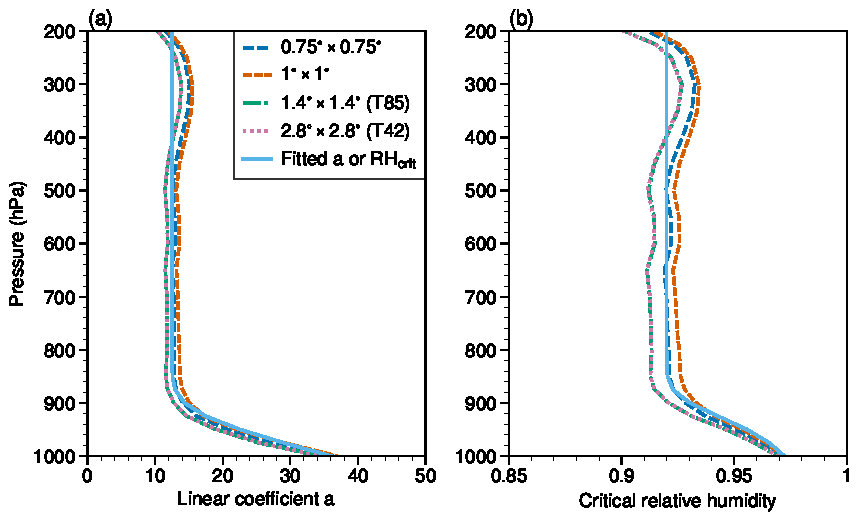
\includegraphics[width=0.8\textwidth]{{figs/simple_cld_scheme/fit_linear_coeff_profile}.pdf}
	\caption{(a) Vertical profiles of the linear coefficient for the relative humidity-based cloud diagnostic scheme, with cloud fraction as a piecewise linear function of relative humidity as shown in Equation \eqref{eq:linear_cf_rh}. The dashed lines with different colors are profiles of $a$ obtained from ERA5 data with various horizontal resolutions. The solid pale blue line denotes the fitted profile used in the model based on the form of Equation \eqref{eq:linear_coeff_a}. (b) is the same as (a), but for the critical relative humidity ($H_{c}$) profiles.}
	\label{fig:linear_coeff_profile}
\end{figure}

%To test the performance of this linear scheme, we also compare it with two other relative-humidity schemes. 
We also provide the \citet{Sundqvist1989} scheme as another option for the relative-humidity schemes, namely
\begin{equation}
	C_s = 1-\sqrt{\frac{1-H}{1-H_{c}}},
	\label{eq:sundqvist}
\end{equation}
where the $H_{c}$ is the critical relative humidity. Here we specify $H_{c}$ as a simple function of height, which is determined by critical relative humidity at three different levels: 0.95 at the surface, 0.85 at 700 hPa, and 0.99 at 200 hPa. Between these levels, the critical relative humidity is linearly interpolated with height. To test the performance of the aforementioned schemes, we compare them with another linear scheme with different form from Equation \eqref{eq:linear_cf_rh}, which is defined as
% Second, we use another linear scheme with different form from Equation \eqref{eq:linear_cf_rh},
\begin{equation}
	C_s = \min\left(1, ~\max \left(0, ~ a \cdot H + b \right)\right),
	\label{eq:linear2}
\end{equation}
where $a$ and $b$ are determined from the least squares fitting of hourly cloud fraction and relative humidity data from ERA5 reanalysis. The cloud fraction in \figref{fig:offline_cld_fraction_test}a is from ERA5 reanalysis at 450 hPa on 12:00 January 01, 2017, while the cloud fractions from three schemes (\figsref{fig:offline_cld_fraction_test}b-\ref{fig:offline_cld_fraction_test}d) are diagnosed from the ERA5 relative humidity field at the same time and level. The linear scheme defined in Equation \eqref{eq:linear2} has two tunable parameters, so one might expect it to perform better than the others. However, the cloud cover can not reach 1 when the grid box is saturated (\figref{fig:offline_cld_fraction_test}c), even though the spatial pattern of cloud cover resembles the ERA5 reanalysis and the global mean value is much closer to the ERA5 compared to the other two schemes. In contrast, the diagnosed cloud amount patterns from Sundqvist scheme (\figref{fig:offline_cld_fraction_test}b) and the linear scheme in the form of Equation \eqref{eq:linear_cf_rh} (\figref{fig:offline_cld_fraction_test}d) are quite similar to the reanalysis (\figref{fig:offline_cld_fraction_test}a), although the cloud cover is a little overestimated in these two schemes. The offline test suggests that the linear scheme in the form of Equation \eqref{eq:linear_cf_rh} is promising to be applied in GCMs.

\begin{figure}
	\centering
	\includegraphics[width=1\linewidth]{{figs/simple_cld_scheme/cmp_sundqvist_linear_with_ecmwf_cc_t_12_lev_20}.png}
	\caption{(a) A snapshot of cloud fraction from ERA5 reanalysis at 450 hPa on 12:00 January 01, 2017. Diagnosed cloud fraction from ERA5 relative humidity field at the same time and level based on the (b) Sundqvist formula, and two linear formulas (c) using Equation \eqref{eq:linear2} and (d) using Equation \eqref{eq:linear_cf_rh}. Note that Equation \eqref{eq:linear_cf_rh} is the form used to determine the large-scale clouds in this study. The global mean cloud fractions are given in the titles.} 
	% [$\min\left(1, ~\max \left(0, ~ a \cdot H + b \right)\right)$],  [i.e., $\min\left(1, ~\max \left(0, ~ a \cdot (H -1) + 1 \right)\right)$]
	\label{fig:offline_cld_fraction_test}
\end{figure}

\subsection{Freeze-dry adjustment}
\label{sec:freezedry}

As we will show in XXXXXXXXXXXXXXXXXXXXXXXXXXXXXX, there are biases in the cloud fraction and cloud radiative effect from the large scale cloud scheme in the polar regions, especially during winter. While it is common for the relative humidity to be near saturation in the Arctic, especially during winter, \citet{Jones2004} showed that there is little subgrid-scale heterogeneity of relative humidity in these stable environments. The small quantity of condensation nuclei in this region further limits the formation of clouds. To alleviate this problem, the `freeze-dry' adjustment, a simple adjustment formula based on specific humidity as indicated by the Equation (2) from \citet{Vavrus2008}, is applied to reduce the cloud fraction under very dry conditions in polar regions. Specifically, if grid mean specific humidity ($q$) is below a threshold ($q_v$), the cloud fraction ($C$) decreases linearly according to the water vapor content:
\begin{equation}
	C= C\cdot f=C \times \max \left(0.15, \min \left(1.0, ~\frac{q}{q_{v}}\right)\right),
	\label{eq:freeze-dry}
\end{equation}
in which the second term is called the freeze-dry factor ($f$). Although the formula is applied globally, the threshold value in Equation \eqref{eq:freeze-dry} ensures that only polar regions will be affected and even there the cloud fraction is adjusted only under very dry conditions.

\begin{figure}[ht]
	\centering
	\includegraphics[width=1\linewidth]{{figs/simple_cld_scheme/feezedry_with_various_qv}.pdf}
	\caption{The $q_v$ vertical profiles with different $n$ and $q_0$. The thick solid and dashed black lines are specific humidity profiles averaged over latitude circles, 60N and 60S, as boundary values of polar regions in Northern and Southern hemispheres, respectively. The thin dashed blue and orange lines are averaged specific humidity profiles over subtropical (30$^\circ$-60$^\circ$N) and tropical (30$^\circ$S-30$^\circ$N) regions in Isca simulation. The other thin solid lines are from Equation \eqref{eq:qv_freeze-dry} with different parameters. In the left, $q_0$ in Equation \eqref{eq:qv_freeze-dry} is 0.006 kg kg$^{-1}$ but $n$ varies from 2 to 4. In the right, $n=2.5$ but $q_0$ varies from 0.003 to 0.006 kg kg$^{-1}$.} 
	% The thick solid and dashed black lines, and the thin dashed blue and orange lines are averaged specific humidity profiles from different regions in Isca simulation. 
	\label{fig:freeze-dry}
\end{figure}

In the original freeze-dry method, Equation \eqref{eq:freeze-dry} was only applied in the lower troposphere \citep{Vavrus2008}. In this study, the freeze-dry formula is applied through the whole atmospheric column, finding that the cloud radiative effect in polar regions is thereby improved. In order to do so, we prescribe the specific humidity threshold $q_v$ in Equation \eqref{eq:freeze-dry} to be a function of pressure with the threshold decreasing exponentially with height as
\begin{equation}
	q_{v} = q_0\left(\frac{p}{p_s}\right)^n.
	\label{eq:qv_freeze-dry}
\end{equation}
Here $q_0$ is the surface specific humidity, $p_s=1000$ hPa is the sea level pressure and $n$ is the power to describe how quickly the specific humidity decreases with height. In \figref{fig:freeze-dry}, different profiles of $q_v$ are shown for the two tunable parameters $n$ and $q_0$. These two parameters are selected to ensure that the freeze-dry adjustment only has effects on polar regions when the $q_v$ profile is applied in Equation \eqref{eq:freeze-dry}. In doing so, the specific humidity profiles from several different regions are plotted in \figref{fig:freeze-dry}. In particular, the profiles of $60^{\circ}$N and $60^{\circ}$S are used to show the specific humidity boundary values of polar regions, and thus the two parameters $q_0$ and $n$ are tuned to follow the boundary profiles. As shown in \figref{fig:freeze-dry}, the $q_v$ profile follows $60^{\circ}$N profile well when the $q_0=0.006$ kg kg$^{-1}$ and $n=2.5$, which can also cover the specific humidity range poleward of $60^{\circ}$S. Therefore in this study the parameters $q_0$ and $n$ are chosen as 0.006 kg kg$^{-1}$ and 2.5, respectively. This threshold works well in current climate setup (see \secref{sec:cld_amt}), but whether it holds under global warming situation still needs further investigation.



\subsection{Low cloud fraction}

Low clouds, especially the subtropical marine stratocumulus clouds, are characterized by high albedo and a cooling effect on climate \citep{Hartmann1992}. Because these clouds cover about 20\% of the subtropical regions even a small change in stratocumulus cloud amount can exert a large radiative forcing at the top of the atmosphere (TOA) \citep{Slingo1990}. However, marine stratocumulus amounts off the west coast of continents have commonly been underestimated and the been an issue in climate models for some time \citep[e.g.,][]{Nam2012, Lauer2013, Dolinar2015}. 

Several proxies or indices for low cloud fraction have been used as predictors for the stratocumulus clouds to try to remedy this \citep[e.g.,][]{Kawai2006, Joshi2015, Collins2004, Guo2014, Kawai2019}, including potential temperature lapse rate ($d\theta/dp$) of the most stable layer below 750hPa \citep{Slingo1987}; lower tropospheric stability \citep[LTS;][]{Klein1993}; estimated inversion strength \citep[EIS;][]{Wood2006}; and the estimated cloud-top entrainment index \citep[ECTEI;][]{Kawai2017}. Recently, \citet{Park2019} proposed a new index, the estimated low-level cloud fraction (ELF), as a predictor for low cloud fraction. ELF (which is a proxy and not necessarily a cloud amount itself) is defined as
%, denoted $\ELF$
\begin{equation}
	\text{ELF} \equiv f \cdot\left[1-\frac{\sqrt{z_{inv} \cdot z_{LCL}}}{\Delta z_{s}}\right],
	\label{eq:ELF}
\end{equation}
where $f$ is the freeze-dry factor defined in \eqref{eq:freeze-dry} with $q_v=0.003$ kg kg$^{-1}$ and $q$ is the surface water vapor specific humidity,  $z_{inv}$ is the inversion height, $z_{LCL}$ is the lifting condensation level of near-surface air, and $\Delta z_{s}= 2750$ m is a constant scale height. As pointed by \citet{Park2019},
$\sqrt{z_{inv} \cdot z_{LCL}}/\Delta z_{s}$ can be rewritten as $z_{LCL}/\Delta z_{s}\cdot \sqrt{1+(z_{inv} -z_{LCL})/z_{LCL}}$, in which $z_{LCL}/\Delta z_{s}$ is a simple but practical proxy of surface moisture, and $(z_{inv}-z_{LCL})/z_{LCL}$ quantifies the strength of the vertical decoupling of the inversion base air from the surface. The ELF predicts that low-level cloud fraction increases as the near-surface air gets more wet (smaller $z_{LCL}$) and as the planetary boundary layer becomes more vertically coupled (smaller $z_{inv}$).

\begin{figure}[ht]
	\centering
	\includegraphics[width=1\linewidth]{{figs/simple_cld_scheme/low_cld_frac_vs_diff_vars_season}.pdf}
	\caption{The relationship between low-level cloud amount and (a) minimum $d\theta/dp$ below 750 hPa, (b) lower tropospheric stability (LTS), (c) estimated inversion strength (EIS), (d) estimated cloud-top entrainment index (ECTEI) and (e) estimated low cloud fraction (ELF) over stratiform cloud regions, including Peru (20$^\circ$S-5$^\circ$N, 80$^\circ$-90$^\circ$W), Namibia (10$^\circ$-30$^\circ$S, 0$^\circ$-15$^\circ$E), California (15$^\circ$-30$^\circ$N, 110$^\circ$-150$^\circ$W), Australia (15$^\circ$-35$^\circ$S, 90$^\circ$-110$^\circ$E), Canary (15$^\circ$-25$^\circ$N, 25$^\circ$-35$^\circ$W), North Pacific (40$^\circ$-5$^\circ$0N, 170$^\circ$-180$^\circ$E), North Atlantic (50$^\circ$-60$^\circ$N, 35$^\circ$-45$^\circ$W) and China (20$^\circ$-30$^\circ$N, 105$^\circ$-120$^\circ$E), which are selected based on \citet{Klein1993}. The data sets are from ERA-Interim reanalysis covering the period from 2013 to 2017. The four points in each region denote the average for different seasons. Linear regression lines and the corresponding fraction of variance ($R^2$) explained by the equation are shown at the top of each plot.}
	\label{fig:fit_low_cld_proxy}
\end{figure}

We have examined the relationship between the seasonal mean low cloud fraction and the various proxies (i.e., $d\theta/dp$, LTS, EIS, ECTEI and ELF) using the ERA-Interim reanalysis data set \citep{Dee2011}. These proxies are derived from the five-year monthly data from 2013 to 2017, including air temperature, surface pressure, surface temperature and low cloud fraction. As shown in \figref{fig:fit_low_cld_proxy}, the regions with typical stratus clouds are selected for the calculation \citep{Klein1993}. The results indicate that the low cloud fraction is linearly related to each indicator in stratus clouds regions, and the ELF tends to have very high correlation with the low-level cloud cover, judging from the fraction of variance ($R^2$) explained by the regression equation. We thus choose to use ELF to construct the diagnostic low cloud fraction formula, that is:
\begin{equation}
	C_{sc} = \min(1, ~\max(0, ~b\times \text{ELF} + c)),
	\label{eq:sc_ELF}
\end{equation}
where $C_{sc}$ is the low stratus cloud fraction, and the two coefficients $b$ and $c$ are treated as tunable parameters. The linear regression formula displayed in \figref{fig:fit_low_cld_proxy}e provides a good starting point for tuning $b$ and $c$ in Equation \eqref{eq:sc_ELF}. After a sensitivity test performed with Isca (the setups will be introduced in \secref{sec:exp_and_data}), we find that if $c$ is specified as the value shown in \figref{fig:fit_low_cld_proxy}e, the shortwave cloud radiative effect is still weak compared to observations. Therefore the parameters $b$ and $c$ are chosen as 1.3 and -0.1 respectively.

In addition, the stratocumulus clouds usually form at the top of planetary boundary layer \citep{Wood2012}, where a strong inversion layer usually exists \citep{Wood2006,Park2019}. However, it is hard for a global model to capture the exact position of the inversion layer due to the limitation of vertical resolution  \citep{Kawai2019}. Care thus needs to be taken to diagnose the marine stratocumulus clouds. First we find the most stable layer below 750 hPa, which is determined by the most negative $d\theta/dp$ \citep{Slingo1987}. Then within the most stable layer, if the lapse rate and vertical velocity satisfy $d\theta/dp<-0.08$ K/hPa and $\omega<0$ hPa/s respectively, then we diagnose stratocumulus clouds at that location. Note that the $d\theta/dp$ threshold is tuneable in our scheme, and it is $-0.125$ K/hPa, as in \citet{Collins2004}.


\subsection{Cloud fraction diagnosis}
\label{sec:cld_amt_diag}
The cloud fraction of a grid box ($C_\mathrm{total}$) is simply defined as the largest fraction of all the clouds within that grid box for simplicity, without separate consideration of their different optical properties:
\begin{equation}
	C_\mathrm{total}=\max(C_s, ~C_{sc}),
	\label{eq:CF_total}
\end{equation}
assuming a horizontal maximum overlap hypothesis \citep[e.g.,][]{Collins2004, Roehrig2020}. $C_s$ and $C_{sc}$ in Equation \eqref{eq:CF_total} are determined by Equations \eqref{eq:linear_cf_rh} and \eqref{eq:sc_ELF} respectively. To assess the performance of the cloud scheme, it is useful to evaluate the total cloud amount and cloud amounts at different levels. In our scheme, the cloud height is determined by cloud top pressures, where those located above 400 hPa are treated as high clouds, those below 700 hPa are defined as low clouds, and in between are middle clouds \citep{Collins2004}. Then, the total, high, middle or low cloud amounts are diagnosed from the maximum-random overlap assumption \citep{Morcrette2000}, which assumes maximum overlap for consecutive cloudy model levels and random overlap for cloud layers that are separated by clear-sky levels.


\section{Effective radius and in-cloud water mixing ratio}

Cloud particles, including liquid droplets and ice crystals, usually have different sizes, shapes and optical properties. In order not to introduce complicated microphysical processes, we do not distinguish them and assume that all particles seen by the radiation scheme are spherical liquid droplets, and ice clouds have a different effective radius from the liquid ones. In this study, the liquid cloud fraction varies with temperature, which only has an influence on the effective radius. %and ice clouds have a different effective radius from liquid ones.

Following \citet{Ose1993} and \citet{Boville2006}, a very simple approach is used to represent the liquid cloud fraction ($f_l$) within a grid box. Specifically, all clouds are assumed to be in liquid form if temperature is warmer than $T_{max}$, and all the condensate is considered as ice if temperature is colder than $T_{min}$. The cloud droplets are in mixed-phase at temperatures between $T_{min}$ and $T_{max}$, and the proportion of liquid cloud in a grid box is defined as a linear function of temperature:
\begin{equation}
	f_{l} =\max\left(0, ~\min\left(1, ~\frac{T-T_{min}}{T_{max}-T_{min}} \right)\right).
	\label{eq:liquid_frac}
\end{equation}
The bounds $T_{min}$ and $T_{max}$ are different in different models. For example, the lower bound ($T_{min}$) is $-40^{\circ}$C in \citet{Ose1993} and \citet{Boville2006}, while it is $-15^{\circ}$C  in \citet{Smith1990}. Observation have shown that cloud liquid water can exist at temperature as low as $-40^{\circ}$C \citep{Heymsfield1993}, although the incidence of liquid water in stratiform clouds is quite low at temperatures below $-15^{\circ}$C \citep{Ryan1996}. The upper bounds ($T_{max}$) are $-5^{\circ}$C for stratiform clouds in \citet{Ose1993}, $-10^{\circ}$C in \citet{Boville2006}, and $0^{\circ}$C in \citet{Smith1990}. Based on the choices in previous studies, $T_{min}$ and $T_{max}$ in Equation \eqref{eq:liquid_frac} are chosen to be $-40^{\circ}$C and $-5^{\circ}$C respectively in this study, but they are to be regarded as adjustable parameters.

The effective radius ($r_{e}$) of droplets within a grid box is defined as a weighted mean of liquid and ice particle radii, with the weights given by the liquid and ice cloud fraction respectively. The radii of liquid and ice particles are selected based on observations. \citet{Stubenrauch2013} assessed cloud properties derived from various satellite data sets, finding that the global mean effective particle radii are about $14$ ($\pm1$) and $25$ ($\pm2$) $\mu m$ for the tops of liquid clouds and for high-level ice clouds, respectively. Therefore these two values are selected to calculate $r_e$,
\begin{equation}
	r_e = 14f_l + 25(1-f_l),
	\label{eq:Reff}
\end{equation}
which is applied globally in the model, although the effective radius of cloud droplets is found a little larger over ocean than over continents in observations \citep{Stubenrauch2013}.

The in-cloud liquid water mixing ratio ($q_l$) is specified as a linear function of the atmospheric temperature, with values of $3\times 10^{-4}$ g kg$^{-1}$ at $220$ K and $q_{l0}=0.18$ g kg$^{-1}$ at $280$ K:
\begin{equation}
	q_l = \max\left(3\times 10^{-4}, ~q_{l0}\times  \min\left(1, ~\frac{T-220}{280-220}\right)\right),
	\label{eq:qcl}
\end{equation}
where the atmospheric temperature $T$ is in units of K. The temperature thresholds, 280 and 220 K,  are selected close to the global averages of liquid and ice cloud top temperature in observations, respectively \citep[Fig. 4 in][]{Stubenrauch2013}. Then the grid mean liquid water specific humidity can be obtained from the product of $q_l$ and cloud fraction. For reference, the equations and parameters used in the cloud scheme are summarized in Table \ref{tab:cld_scheme_summary}. 

\begin{sidewaystable}
	\caption{Summary of the diagnostic cloud scheme.}
	\centering
	\renewcommand{\arraystretch}{1.5}
	\begin{tabular}{c c p{6cm} p{7cm} l} 
		\hline
		%Symbol & Range /Units & Definition & Diagnostic formula & Tunable parameters \\
		\multirow{2}{*}{Symbol} & Range  & \multirow{2}{*}{Definition} & \multirow{2}{*}{Diagnostic formula} & \multirow{2}{*}{Tunable parameters} \\
		& /Units & & & \\
		\hline % \multirow{3}{*}{
		\multirow{3}{*}{$C_s$} & \multirow{3}{*}{[0, 1]} & \multirow{3}{*}{Large-scale cloud fraction} & $\min\left(1, ~\max \left(0, ~a \cdot (H-1) + 1 \right)\right)$,&  \multirow{2}{*}{$a_s=36$, $a_t=13$, $n=12$} \\
		& &  &	$a=a_t + (a_s-a_t)\exp{\left[1-\left( \frac{p_s}{p} \right)^{n} \right]}$& \\ \cline{4-5}
		& &  &	$\min\left(1, ~\max \left(0, ~1-\sqrt{\frac{1-H}{1-H_{c}}} \right)\right)$ & $H_c$: function of height  \\
		\hline
		\multirow{2}{*}{$f$}  & \multirow{2}{*}{[0.15, 1]} & \multirow{2}{*}{Freeze-dry adjustment factor} & $\max \left(0.15, \min \left(1.0, ~\frac{q}{q_{v}}\right)\right)$, & \multirow{2}{*}{$q_0=6 ~g~kg^{-1}$, $n=2.5$} \\
		& & & $q_{v}= q_0\left(\frac{p}{p_s}\right)^n$ & \\
		\hline 
		\multirow{2}{*}{$C_{sc}$} & \multirow{2}{*}{[0, 1]} & \multirow{2}{*}{Low cloud fraction} & $\min(1, ~\max(0, ~b\times \text{ELF} +c))$, & $b=1.3$, $c= -0.1$  \\
		& & &  $\text{ELF}=f \cdot\left[1-\sqrt{z_{inv} \cdot z_{LCL}}/{\Delta z_{s}}\right]$  & $q_v=3~g~kg^{-1}$ in $f$ \\
		\hline 
		\multirow{2}{*}{$f_l$} & \multirow{2}{*}{[0, 1]}  & \multirow{2}{*}{Liquid cloud fraction} & $\max\left(0, ~\min\left(1, ~\frac{T-T_{min}}{T_{max}-T_{min}} \right)\right)$, & \multirow{2}{*}{$T_{min}=-40$, $T_{max}=-5^\circ C$} \\
		& & & ($T$ in units of $^\circ C$) & \\
		$r_e$ & $\mu$m &	Effective radius & $r_{e\_liq}f_l + r_{e\_ice}(1-f_l)$ & $r_{e\_liq}=14$, $r_{e\_ice}=25$ $\mu m$ \\
		\hline
		\multirow{2}{*}{$q_l$} & \multirow{2}{*}{g kg$^{-1}$} & \multirow{2}{*}{In-cloud liquid water mixing ratio} & $\max\left(3\times 10^{-4}, ~q_{l0}\times \min\left(1, ~\frac{T-220}{280-220}\right)\right)$, &
		\multirow{2}{*}{$q_{l0}=0.18~g~kg^{-1}$} \\
		& & & ($T$ in units of $K$) & \\
		\hline
	\end{tabular}
	\label{tab:cld_scheme_summary}
\end{sidewaystable}

\section{Radiation}
\label{sec:radiation}

Radiative transfer is handled by the SOCRATES (Suite of Community Radiation Codes based on Edwards \& Slingo) radiation scheme \citep{Edwards1996, Manners2015}. Spectral files with 9 longwave bands and 6 shortwave bands are used to calculate the radiation transfer, which are those used in the Unified Model's Global Atmosphere version 7 \citep{Walters2019}. The cloud fraction, effective radius of cloud particle and liquid water mixing ratio in each grid are passed to it, then the radiation fluxes under all-sky and clear-sky conditions are obtained, which are used to analyze the energy balance and to calculate the cloud radiative effect \citep{Ramanathan1989, Li2017} at the top of the atmosphere. 



\section{Data sets}

To evaluate the performance of the cloud scheme, several observations and reanalysis data sets are employed. Specifically, the 10-year monthly data (1995 to 2014) of International Satellite Cloud Climatology Project (ISCCP) H-series products \citep{Young2018} is used to evaluate the simulated cloud amounts. The cloud fraction from Isca simulations is compared to retrieved cloud fraction from GCM-Oriented Cloud-Aerosol Lidar and Infrared Pathfinder Satellite Observations (CALIPSO) Cloud Observations product (GOCCP) \citep{Chepfer2010}. To examine the radiative flux simulated in Isca, monthly data from January 2001 to December 2018 from Clouds and Earth's Radiant Energy System (CERES) Energy Balanced and Filled (EBAF) Edition 4.1 product \citep[CERES-EBAF hereafter;][]{Loeb2018} are used for comparison. The cloud water path is from the CloudSat 2B-CWC-RO Release P1\_R05 data product \citep{Austin2009} from 2012 to 2016, which can better represent cloud liquid and ice water path over high latitudes than CERES-EBAF data set, owing to its explicit determination of cloud phase \citep{Lenaerts2017}. In addition, monthly vertical pressure velocity from ERA-Interim reanalysis and radiative flux data from CERES-EBAF data sets covering the period 2008-2017 are also adopted to quantify the LW CRE over the tropics.

In order to demonstrate how this cloud scheme performs with respect to more comprehensive models, the monthly mean radiative fluxes at clear-sky and all-sky conditions in historical simulation (1996 to 2005) from various CMIP5 models are also shown for the names of models). All the data sets are remapped to T42 resolution when necessary for a direct comparison with Isca simulations.

% %\chapter{Evaluation of the Cloud Scheme}

\section{Introduction}

In this chapter, the simulated climatology from the simple cloud scheme described in \chapref{chp:simple_cld_scheme} is presented here. \secref{sec:exp_setup_and_dataset} introduces the experiment setup and data sets used in this chapter. The evaluation will focus on features of cloud fraction, cloud water path and cloud radiative effects, including their vertical profile (if any), spatial pattern, zonal mean structure and seasonal cycles.

\section{Data and methods}
\label{sec:exp_setup_and_dataset}

\subsection{Experiment setup}

Our simulations are AMIP-type, that is they follow those used in the Atmospheric Model Intercomparison Project. They are performed with a realistic Earth-continental configuration following \citet{Thomson2018} (which is derived from the ERA-Interim land mask and topography \citep{Dee2011}) and at a horizontal resolution of T42 (roughly 2.8$^\circ$ $\times$ 2.8$^\circ$) with 25 vertical levels. The sea surface temperature is fixed at AMIP climatology \citep{Taylor2000sea}, which is annually repeating but seasonally varying. The sea ice data is also from AMIP, but is averaged over all years and months to obtain an annual mean distribution, as in \citet{Thomson2018}. The albedo in sea ice regions increases linearly with the sea ice concentration with the maximum of 0.7. The surface albedo of the other parts except the sea ice is fixed as 0.11. The insolation includes a seasonal and diurnal cycle, with a solar constant of 1360 Wm$^{-2}$. The convection parameterization used in this study is the simplified Betts--Miller scheme from \citet{Frierson2007}. 

The SOCRATES (Suite of Community Radiation Codes based on Edwards \& Slingo) radiation scheme \citep{Edwards1996, Manners2015} is employed for the radiation transfer calculation as in \citet{Thomson2019}. Spectral files with 9 longwave bands and 6 shortwave bands are used, which are those used in the Unified Model's Global Atmosphere version 7 \citep{Walters2019}. The cloud fraction, effective radius of cloud particle and liquid water mixing ratio in each grid are passed to it, then the radiation fluxes under all-sky and clear-sky conditions are obtained, which are used to analyze the energy balance and to calculate the cloud radiative effect \citep{Ramanathan1989, Li2017} at the TOA.

In order to compare the roles of different cloud parameterization schemes, simulations are performed with the combination of different clouds or different adjustment methods as shown in Table \ref{tab:exps}. The simulation with large-scale clouds only is denoted as the LS simulation. The run with large-scale clouds and freeze-dry adjustment is called the FD simulation. The run performed with large-scale clouds, freeze-dry adjustment and marine low stratiform clouds is referred as the ALL simulation. The simulations are all run for 20 years, with the first 10 years treated as spin-up and discarded.

\begin{table}
	\caption{Summary of the Isca fixed-SST simulations}
	\vspace{0.5em}
	\centering
	\renewcommand{\arraystretch}{1.3}
	\begin{tabular}{ll}
		\hline
		Experiment & Description \\
		\hline
		LS  & Run with large-scale clouds only. \\ 
		FD  & Based on the LS run, with freeze-dry adjustment also applied. \\ 
		\multirow{2}{*}{ALL} & The marine low-level clouds are also included on top of the \\
		    & FD run.  \\
		\multirow{3}{*}{Linear\_X} 	&  X is one of the LS, FD and ALL runs, in which the large-scale \\
		& clouds are diagnosed from a linear function of RH as defined\\
		& in \eqref{eq:linear_cf_rh}. \\
		\multirow{2}{*}{Sundqvist\_X} & Same as Linear\_X, but with \citet{Sundqvist1989} scheme\\ 
		& as defined in \eqref{eq:sundqvist}.\\
		\hline
	\end{tabular}
	\label{tab:exps}
\end{table}

\subsection{Data sets}
To evaluate the performance of the cloud scheme, several observations and reanalysis data sets are employed. Specifically, the 10-year monthly data (1995 to 2014) of International Satellite Cloud Climatology Project (ISCCP) H-series products \citep{Young2018} is used to evaluate the simulated cloud amounts. The cloud fraction from Isca simulations is compared to retrieved cloud fraction from GCM-Oriented Cloud-Aerosol Lidar and Infrared Pathfinder Satellite Observations (CALIPSO) Cloud Observations product (GOCCP) \citep{Chepfer2010}. To examine the radiative flux simulated in Isca, monthly data from January 2001 to December 2018 from Clouds and Earth's Radiant Energy System (CERES) Energy Balanced and Filled (EBAF) Edition 4.1 product \citep[CERES-EBAF hereafter;][]{Loeb2018} are used for comparison. The cloud water path is from the CloudSat 2B-CWC-RO Release P1\_R05 data product \citep{Austin2009} from 2012 to 2016, which can better represent cloud liquid and ice water path over high latitudes than CERES-EBAF data set, owing to its explicit determination of cloud phase \citep{Lenaerts2017}. In addition, monthly vertical pressure velocity from ERA-Interim reanalysis and radiative flux data from CERES-EBAF data sets covering the period 2008-2017 are also adopted to quantify the longwave CRE over the tropics.

In order to demonstrate how this cloud scheme performs with respect to more comprehensive models, the monthly mean radiative fluxes at clear-sky and all-sky conditions in historical simulation (1996 to 2005) from various CMIP5 models are also shown for the names of models). All the data sets are remapped to T42 resolution when necessary for a direct comparison with Isca simulations.

\section{Simulated cloud amount}
\label{sec:cld_amt}

The global mean cloud amount and radiative components for the observations and Isca simulations are summarized in Table \ref{tab:global_mean_climate}. 

\begin{sidewaystable}
	\caption{Global and annual mean climatological properties of observations and different Isca simulations, which are summarized in Table \ref{tab:exps}. The net fluxes in the table are positive downward. }
	\vspace{0.5em}
	\centering
	\renewcommand{\arraystretch}{1.5}
	% https://tex.stackexchange.com/questions/209802/footnote-in-table-environment
	% use this package for footnote
	\begin{threeparttable}
	%\begin{tabular}{lrrrrrrr}
	\begin{tabular}{lccccccc}
    	\hline
    	{} &   Obs &  Linear\_LS &  Linear\_FD &  Linear\_ALL &  Sundqvist\_LS &  Sundqvist\_FD &  Sundqvist\_ALL \\
    	\hline
    	Low cloud amount (\%)      &  28.0\tnote{a} &       54.6 &       49.3 &        48.6 &          53.8 &          48.3 &           47.5 \\
    	Middle cloud amount (\%)   &  20.8\tnote{a} &       25.9 &       20.8 &        20.6 &          25.3 &          20.2 &           20.0 \\
    	High cloud amount (\%)     &  12.8\tnote{a} &       42.3 &       30.4 &        30.4 &          35.9 &          25.5 &           25.5 \\
    	Total cloud amount (\%)    &  65.3\tnote{a} &       75.6 &       66.4 &        66.0 &          72.4 &          63.3 &           62.6 \\
    	TOA net SW flux (Wm$^{-2}$)  & 241.3\tnote{b} &      226.8 &      229.2 &       229.6 &         228.7 &         231.2 &          231.5 \\
    	TOA net LW flux (Wm$^{-2}$)  & 240.3\tnote{b} &      220.4 &      224.8 &       224.9 &         223.3 &         227.6 &          227.4 \\
    	TOA net flux (Wm$^{-2}$)     &   1.0\tnote{b} &        6.4 &        4.5 &         4.7 &           5.4 &           3.6 &            4.0 \\
    	TOA SW CRE (Wm$^{-2}$)       & -45.8\tnote{b} &      -58.8 &      -56.3 &       -56.0 &         -56.9 &         -54.3 &          -54.1 \\
    	TOA LW CRE (Wm$^{-2}$)       &  28.0\tnote{b} &       36.4 &       31.3 &        31.0 &          33.3 &          28.5 &           28.3 \\
    	TOA net CRE (Wm$^{-2}$)      & -17.8\tnote{b} &      -22.4 &      -25.0 &       -24.9 &         -23.5 &         -25.8 &          -25.8 \\
    	Cloud water path (gm$^{-2}$) & 119.3\tnote{c} &      147.0 &      129.7 &       130.4 &         144.1 &         127.1 &          126.8 \\
    	\hline
    \end{tabular}
    
    \begin{tablenotes}
      \item[a] The observed cloud amounts are from ISCCP H-series \citep{Young2018} product (1995--2014)
      \item[b] The radiative fluxes and cloud radiative effects (CREs) at the TOA are from CERES-EBAF \citep{Loeb2018} data set (2001--2018)
      \item[c] The cloud water path is from CloudSat 2B-CWC-RO Release P1\_R05 \citep{Austin2009} data product (2012--2016)
     \end{tablenotes}
     
    \end{threeparttable}
    \label{tab:global_mean_climate}
\end{sidewaystable}

The global mean cloud fraction profiles from CALIPSO-GOCCP, ERA-Interim reanalysis and Isca simulations are displayed in \figref{fig:cld_fraction_profile}a. The cloud fractions from all the Isca simulations are higher than observations, especially in the middle and high levels. The FD simulations are closer to observations than the LS simulations, which is true for both the linear and Sundqvist schemes. Regarding the annual and zonal mean profiles, a striking feature is that the LS simulations from both linear and Sundqvist schemes overestimate the cloud fraction at high latitudes (\figsref{fig:cld_fraction_profile}d and \ref{fig:cld_fraction_profile}g) compared to the observation (\figref{fig:cld_fraction_profile}b) and reanalysis (\figref{fig:cld_fraction_profile}c). These biases are mitigated in the FD simulations (\figsref{fig:cld_fraction_profile}e and \ref{fig:cld_fraction_profile}h), as the cloud fractions are limited due to insufficient water vapor content at high latitudes. Despite more clouds being diagnosed at low levels over the eastern subtropical ocean regions, the zonal mean cloud fraction profiles in the ALL simulations (\figsref{fig:cld_fraction_profile}f and \ref{fig:cld_fraction_profile}i) are generally similar to those from the FD simulations. In summary, the cloud fraction profiles have been improved from the LS to ALL simulations due to the freeze-dry adjustment and the extra low clouds. However, the cloud fractions are still overestimated in high levels over the subtropics, which could possibly explain the CRE biases over these regions.

\begin{figure}[ht]
	\centering
	\includegraphics[width=1.\linewidth]{{figs/evaluation_of_cld_scheme/cloud_zonal_mean_vert_profiles}.pdf}
	\caption{(a) The annual and global mean of cloud fraction profiles from the CALIPSO-GOCCP (thick blue solid line), ERA-Interim reanalysis (thick orange solid line) and different Isca simulations, including linear\_LS (blue dotted), linear\_FD (orange dash-dotted), linear\_ALL (green dashed), Sundqvist\_LS (pink dotted), Sundqvist\_FD (yellow dash-dotted) and Sundqvist\_ALL (azure dashed). (b-i) Same as in (a), but for annual and zonal mean of cloud fraction profiles.}
	\label{fig:cld_fraction_profile}
\end{figure}

In addition to the cloud fraction profiles, the geographic patterns of cloud amount, diagnosed from the random-maximum overlap assumption (\secref{sec:cld_amt_diag}), are also compared with observations. For example, the annual mean spatial patterns of low cloud amount from three different simulations (LS, FD and ALL) with linear RH cloud scheme, ISCCP-H data set, and the differences between them are shown in \figref{fig:low_cld_amt}. It should be pointed out that the simulated cloud amounts are compared to the satellite retrievals directly in this study, because the cloud simulator \citep[e.g.,][]{Bodas2011} has not been implemented in Isca. This may bring in some inconsistencies, but it does provide a useful first look of the cloud amount diagnosis.

\begin{figure}[ht]
	\centering
	\includegraphics[width=1\linewidth]{{figs/evaluation_of_cld_scheme/low_cld_amt_isca_obs}.pdf}
	\caption{The annual mean geographic patterns of low cloud amount (\%) from the (a) LS, (b) FD, (c) ALL simulations with the linear scheme as well as (d) observation (ISCCP-H), and the differences between the (e) FD and LS, (f) ALL and FD, (g) LS and observation, (h) FD and observation, and (i) ALL and observation. Note that (a-d) use the upper color scale, (e-f) use the middle one, and (g-i) use the one at the bottom.}
	\label{fig:low_cld_amt}
\end{figure}

One evident feature of the low cloud amount in observations is that marine stratocumulus clouds dominate the areas off the west coast of continents (\figref{fig:low_cld_amt}d), related to the subsidence branch of the Hadley Cell \citep{Wood2012}. The predominantly downward motion in these regions generally suppresses cloud formation in the middle and upper troposphere, but due to the abundance of water vapor near the ocean surface, clouds form at the top of convective boundary layers. However, these marine low clouds are too far from the coasts in the LS simulation compared to the observations (\figref{fig:low_cld_amt}a). Looking at the differences between LS simulation and observations (\figref{fig:low_cld_amt}g), the low cloud amount is underestimated by about 20\% off the west coast of Peru. In fact, these are well-known biases in CMIP5 models \citep{Dolinar2015}. Another problem of the LS simulation is the overproduction of low cloud amount in polar regions (\figref{fig:low_cld_amt}g). For example, LS simulation produces more than 40\% low cloud over Arctic region. %which is a similar but less severe bias in mid-latitudes.

In contrast, the cloud fractions in the FD and ALL simulations are adjusted by the freeze-dry method (see \secref{sec:freezedry}), which is mainly designed to reduce the unrealistic cloud amount in polar regions. Thus there is a reduction of low cloud amount over high latitudes in these two simulations (\figsref{fig:low_cld_amt}h and \ref{fig:low_cld_amt}i), although some positive biases still exist there. Compared with the LS simulation directly, the FD simulation can reduce the low cloud amount by more than 20\% over polar regions (\figref{fig:low_cld_amt}e), showing a better agreement with the observations. The ALL simulation can further diagnose the marine stratus clouds off the west coast of continents through the predictor ELF, making the low clouds distribution closer to the observation (\figref{fig:low_cld_amt}c). It is noted that pronounced changes occur off the west coasts of Peru, California and Namibia in the ALL simulation, where the cloud fraction increases over 20\% (\figref{fig:low_cld_amt}f) than the FD run. As shown in Table \ref{tab:global_mean_climate}, the global mean low cloud amount decreases from 54.6\% to 48.6\% from the LS to ALL simulations with the linear RH scheme, which is closer to the observed value (28\%). The changes of total cloud amount in these simulations (not shown here) are similar, and the global mean value decreases from 75.6\% (the LS run) to 66.0\% (the ALL run) for the linear RH scheme (Table \ref{tab:global_mean_climate}).

\begin{figure}[ht]
	\centering
	\includegraphics[width=1.0\linewidth]{{figs/evaluation_of_cld_scheme/cloud_amount_in_arctic_region}.pdf}
	\caption{The seasonal cycle of (a) low and (b) total cloud amount (\%) over the Arctic region ($60^\circ$-$90^\circ$N) from the LS (solid lines) and FD (dashed lines) simulations, where the freeze-dry adjustment method is applied in the FD simulations. The green and pink colors denote the experiments performed with the linear and Sundqvist cloud schemes respectively.}
	\label{fig:cld_amt_freeze-dry}
\end{figure}

The above analyses have shown that the freeze-dry method can improve the spatial patterns of annual mean cloud amount, with these changes being especially pronounced  during winter time \citep[as also noted by][]{Vavrus2008}. Figure \ref{fig:cld_amt_freeze-dry} illustrates the annual cycle of low and total cloud amounts over Arctic region from both linear RH and Sundqvist schemes. In the LS simulations, both the low and total cloud amounts are nearly at the same level throughout the year. However, a striking feature in the FD simulations is that the cloudiness declines rapidly during boreal winter but remains almost unchanged in warm and moist summer, which in fact is more realistic compared to observations as pointed by \citet{Vavrus2008}.


\section{Simulated cloud water path}
\label{sec:cwp}

\begin{figure}[ht]
	\centering
	\includegraphics[width=1\linewidth]{{figs/evaluation_of_cld_scheme/cwp_isca_obs}.pdf}
	\caption{Same as \figref{fig:low_cld_amt}, but for the spatial patterns of total cloud water path (CWP; gm$^{-2}$). The observed climatology of CWP is derived from the CloudSat data set.}
	\label{fig:cwp}
\end{figure}

The cloud water path (CWP) measures the total amount of cloud water within a column and is defined as the integral of cloud water content from surface ($p=p_s$) to TOA ($p=0$) \citep[Eq. 9.30 in][]{Stensrud2009}, and it can be expressed as follows if the hydrostatic equilibrium is assumed:
\begin{equation}
	CWP = \int_{p=0}^{p=p_s} C\cdot q_l\frac{dp}{g},
	\label{eq:cwp}
\end{equation}
where $q_l$ is the in-cloud liquid water mixing ratio specified in Equation (\ref{eq:qcl}), $C$ is the cloud fraction within a grid box, $g$ is the acceleration due to gravity and $p$ is the pressure. The global and annual mean CWP in the LS simulation from linear RH scheme is 147.0 gm$^{-2}$, which is larger than the observed global mean result (119.3 gm$^{-2}$, see Table \ref{tab:global_mean_climate}). As displayed in \figref{fig:cwp}, one obvious bias in the spatial pattern in the LS simulation is the overestimation of CWP at high latitudes. For instance, these biases can be even more than 90 gm$^{-2}$ in the polar regions (\figsref{fig:cwp}a and \ref{fig:cwp}g). Such an overestimation is also evident in cloud amount over the polar regions (e.g. \figref{fig:low_cld_amt}g), suggesting that the adjustment of cloud fraction probably reduces the CWP biases there. Indeed, incorporating the freeze-dry method into the simulation produces a large change in the CWP spatial pattern, with a reduction over 60 gm$^{-2}$ over polar regions (\figsref{fig:cwp}b, \ref{fig:cwp}e and \ref{fig:cwp}h). The CWP biases off the west coast of continents are reduced in the ALL simulation due to the increase of the low cloud fraction there. For example, the CWP over Peruvian and Californian coasts in the ALL simulation increases at least 20 gm$^{-2}$ when compared to the LS simulation (\figref{fig:cwp}e).

\section{Simulated cloud radiative effect}

\begin{figure}[ht]
	\centering
	\includegraphics[width=1\linewidth]{{figs/evaluation_of_cld_scheme/toa_sw_cre_isca_obs}.pdf}
	\caption{Same as \figref{fig:low_cld_amt}, but for shortwave (SW) cloud radiative effect (CRE) (Wm$^{-2}$) at TOA. The observed SW CRE is from CERES-EBAF data set.}
	\label{fig:toa_sw_cre}
\end{figure}

\begin{figure}[ht]
	\centering
	\includegraphics[width=1.\linewidth]{{figs/evaluation_of_cld_scheme/SW_CREs_improvement_linear}.pdf}
	\caption{(a) The regional mean SW CRE biases from the FD and ALL simulations with with linear RH scheme in five different subtropical ocean regions off the west coast of continents, whose ranges are defined in the caption of \figref{fig:fit_low_cld_proxy}. (b) The relationship of regional mean SW CRE and low cloud amount changes in the FD and ALL simulations, and the changes are calculated as their differences (i.e., ALL-FD).}
	\label{fig:swcre_marine_sc}
\end{figure}

The CRE is defined as the differences in TOA radiative fluxes between clear-sky and all-sky conditions \citep[e.g.,]{Ramanathan1989,Li2017}. Specifically, the simulated LW CRE is derived from the difference between the outgoing longwave radiation flux under clear-sky and all-sky conditions, and the SW CRE is computed from the difference in reflected SW flux under clear-sky and all-sky conditions. The net CRE is defined as the sum of LW and SW CREs.

\subsection{Spatial patterns of cloud radiative effect}

The global mean SW CRE from the LS simulation is -58.8 Wm$^{-2}$, which is much larger than the observed value of -45.8 Wm$^{-2}$ from CERES-EBAF (Table \ref{tab:global_mean_climate}). Compared to the observed SW CRE (\figref{fig:toa_sw_cre}c), the LS simulation can reproduce the general features of spatial patterns (\figref{fig:toa_sw_cre}a), although it fails to grasp some key features. For example, SW CRE is underestimated by over 30 Wm$^{-2}$ in eastern subtropical ocean basins off the west coast of Peru and over 15 Wm$^{-2}$ off the west coast of California (\figref{fig:toa_sw_cre}g), consistent with the insufficient low cloud amounts in these marine stratocumulus areas (\figref{fig:low_cld_amt}g). These biases also exist in the FD simulation (\figsref{fig:toa_sw_cre}b and \ref{fig:toa_sw_cre}h), as the freeze-dry method can only adjust the cloud amount over high latitudes. As shown in sections \ref{sec:cld_amt} and \ref{sec:cwp}, the low cloud amount and CWP in these regions increase in the ALL simulation, which is thus expected to improve the SW CRE biases. In fact, the differences between the ALL and FD simulations show that the SW CREs reduce by more than 10 Wm$^{-2}$ off the Californian, Peruvian and Namibian coasts (\figref{fig:toa_sw_cre}f). Consequently, the positive biases in SW CRE over eastern subtropical ocean regions are reduced, although some smaller positive biases still remain (\figref{fig:toa_sw_cre}i). The SW CRE biases from the LD and ALL simulations in the five marine stratocumulus clouds regions (defined in \figref{fig:fit_low_cld_proxy}) are quantified in \figref{fig:swcre_marine_sc}a. It is clear that these biases are reduced in all the locations, which is closely linked to the increase of low cloud amount over these regions (\figref{fig:swcre_marine_sc}b).

Another problem of the SW CRE in the LS simulation is that it is too negative in trade wind cumulus regions, Southern Ocean and northern Pacific Ocean (\figref{fig:toa_sw_cre}g), which is associated with the excessive clouds over these regions (\figref{fig:low_cld_amt}g). The freeze-dry adjustment has reduced the cloud amount at high latitudes, making the SW CRE in the Southern Ocean less negative compared to the LS simulation (\figsref{fig:toa_sw_cre}e and \ref{fig:toa_sw_cre}h). In the end, the SW CRE in the ALL simulation becomes more realistic compared to observations, and the global mean value (-56.0 Wm$^{-2}$) is closer to the observed value (-45.8 Wm$^{-2}$) from CERES-EBAF (Table \ref{tab:global_mean_climate}).

\begin{figure}[ht]
	\centering
	\includegraphics[width=1.\linewidth]{{figs/evaluation_of_cld_scheme/toa_lw_cre_isca_obs}.pdf}
	\caption{Same as \figref{fig:toa_sw_cre}, but for LW CRE (Wm$^{-2}$) at TOA. }
	\label{fig:toa_lw_cre}
\end{figure}

The LS simulation reproduces the general spatial pattern of the observed LW CRE (\figsref{fig:toa_lw_cre}a and \ref{fig:toa_lw_cre}d). However, the radiative effect is too strong, especially in the polar regions and also over the maritime continent regions (\figsref{fig:toa_lw_cre}a and \ref{fig:toa_lw_cre}d), which is also illustrated by the positive biases over these regions (\figref{fig:toa_lw_cre}g). The LW CRE in the LS simulation is overestimated by over 30 Wm$^{-2}$ in the Arctic and over 15 Wm$^{-2}$ in tropical regions. As discussed in previous sections, the cloud fraction, as well as the CWP in polar regions, decreases in the FD simulation compared to the LS run. Therefore, the LW CRE is improved over these regions (\figsref{fig:toa_lw_cre}b and \ref{fig:toa_lw_cre}h), where the bias in polar region is reduced by more than 15 Wm$^{-2}$ (\figref{fig:toa_lw_cre}e). Nevertheless, there is still a small positive bias over the Arctic and tropical regions. Compared to the FD simulation, the changes in the ALL simulation has little effect on LW CRE (\figref{fig:toa_lw_cre}f). After these improvements, the spatial patterns of LW CRE in the FD and ALL simulations become more similar to the observations, and the global mean CRE drops from 36.4 Wm$^{-2}$ to 31.0 Wm$^{-2}$, much closer to global mean result from observations (Table \ref{tab:global_mean_climate}).

\begin{figure}[ht]
	\centering
	\includegraphics[width=1\linewidth]{{figs/evaluation_of_cld_scheme/linear_cldamt_lwcre_binned_by_omega_year_ocean}.pdf}
	\caption{(a) The vertical pressure velocity field at 500 hPa ($\omega_{500}$) over tropical oceans between 30$^\circ$S and 30$^\circ$N from the linear\_LS simulation. (b) The probability density functions (PDFs) of the 500 hPa large-scale vertical velocity ($\omega_{500}$) over the tropical ocean regions defined in (a), where the vertical bars indicate one standard deviation of the annual mean data. (c) The low, high cloud amounts and (d) the TOA LW CRE in different dynamical regimes binned by $\omega_{500}$. The 10-year (2005-2014) observed cloud amounts from ISCCP-H and the LW CRE from CERES-EBAF are binned by $\omega_{500}$ from ERA-Interim reanalysis data set (black lines). The results from the LS, FD and ALL simulations with the linear RH scheme are represented by blue, orange and green lines, respectively.}
	\label{fig:pdf_lw_cre}
\end{figure}

To further quantify the simulated LW CRE at TOA over the tropical ocean regions (30$^{\circ}$S-30$^{\circ}$N), following the method employed in \citet{Bony2004} and \citet{Bony2005}, we first define the upwelling and downwelling regimes based on the vertical pressure velocity at 500 hPa ($\omega_{500}$, \figref{fig:pdf_lw_cre}a), and then evaluate the LW CRE over these regimes. $\omega_{500}$ is a measure of the large-scale atmospheric circulation, where the regions with positive $\omega_{500}$ are associated with the subsidence movement, while those with negative $\omega_{500}$ are related to large-scale atmospheric ascent. The PDFs of $\omega_{500}$ from the ERA-Interim reanalysis and Isca simulations (LS, FD and ALL runs) are displayed in \figref{fig:pdf_lw_cre}b. The PDFs of the Isca simulations generally follows the observations, albeit the Isca simulations have more weakly ascending regions and fewer weakly descending regions. The peak values of PDFs are located at 5-20 hPa/day, consistent with the results from \citet{Bony2004}.

Figures \ref{fig:pdf_lw_cre}c and \ref{fig:pdf_lw_cre}d illustrate the high/low cloud amounts and LW CRE at the TOA over different dynamical regimes over tropical oceans, respectively. The observed cloud amount and LW CRE are from ISCCP-H and CERES-EBAF data sets respectively, both covering the period from 2005 to 2014 with the regimes being defined by the $\omega_{500}$ from ERA-Interim. The regimes with stronger convective activity, related to the magnitude of $\omega_{500}$ in ascending regions ($\omega_{500}<0$), usually have a larger amount of high clouds and thus stronger LW CREs. All the LW CREs from the three simulations are close to the observed values over the weak upwelling and subsidence regions. However, the LW CREs from the LS simulation deviate from the observations in strong ascending regions ($\omega_{500}<-20$ hPa day$^{-1}$). Furthermore, this discrepancy increases with the magnitude of $\omega_{500}$ in ascending regions ($\omega_{500}<0$). It is noted that the large biases of LW CRE over ascending regions is reduced slightly in the FD and ALL simulations, associated with the decrease of high clouds over those regimes (\figref{fig:pdf_lw_cre}c). However, the positive biases still exist at the strong convection regions. 

\begin{figure}[ht]
	\centering
	\includegraphics[width=1.\linewidth]{{figs/evaluation_of_cld_scheme/toa_net_cre_isca_obs}.pdf}
	\caption{Same as \figref{fig:toa_sw_cre}, but for net CRE (Wm$^{-2}$) at TOA.}
	\label{fig:toa_net_cre}
\end{figure}

Finally, the spatial pattens of net CREs at the TOA are presented in \figref{fig:toa_net_cre}, where we can see that the positive biases in the LS simulation mainly occur in the polar regions and subtropical eastern ocean regions. There are also small negative biases in subtropical and extratropical regions. The positive biases in net CRE in the LS simulation are related to the cloud amount biases in these regions, as we have seen in the SW and LW CRE fields. Clearly, the biases in polar regions are reduced greatly in the FD simulations (\figsref{fig:toa_net_cre}b, \ref{fig:toa_net_cre}e and \ref{fig:toa_net_cre}h) due to the freeze-dry method. Additionally, the positive biases off the west coasts of continents in subtropics can be mitigated in the ALL simulation (\figref{fig:toa_net_cre}i), making the spatial pattern closer to CERES-EBAF, although there are still slight positive biases in polar regions.

\subsection{Zonal mean structure}
\begin{figure}[ht]
	\centering
	\includegraphics[width=1\linewidth]{{figs/evaluation_of_cld_scheme/cmp_zonal_toa_CRE_cmip_isca}.pdf}
	\caption{Zonally averaged distribution of the TOA (a) SW, (b) LW and (c) net CREs from CERES-EBAF Ed4.1 (blue solid line), ERA-Interim reanalysis (orange solid line), CMIP5 models (thin gray solid lines for each model and black solid line for multimodel mean) and different Isca simulations (dashed/dotted color lines, listed in legend).}
	\label{fig:zonal_mean_cre}
\end{figure}

To further study their latitudinal variations, the zonally averaged SW, LW and net CREs from Isca simulations, CMIP5 simulations, satellite observation and reanalysis data set are shown in \figref{fig:zonal_mean_cre}. For the SW CRE (\figref{fig:zonal_mean_cre}a), the general latitudinal variations can be captured by all the Isca simulations, but the magnitude is larger than observations. The largest discrepancy in the LS simulations occurs in the mid-latitudes, especially in the Southern hemisphere, which is likely arising from the excessive cloud amount over these regions (\figref{fig:low_cld_amt}g). The improvement of cloud amount biases in the FD and ALL simulations contributes to the improvement of SW CRE over the extratropics. However, the difference of zonal mean SW CREs between the FD and ALL simulations is slight, although the SW CRE biases over eastern subtropical ocean regions are reduced in the ALL run (\figref{fig:toa_sw_cre}f). In addition, the remaining SW CRE biases, as well as the low cloud amount biases, in the ALL simulation over the subtropics and extratropics might be alleviated by an `omega correction’, namely a reduction of the low cloud fraction if subsidence is strong \citep[e.g.,]{Gordon1992}, but the effects are mixed and we do not include that process in these results.

Regarding to the LW CREs (\figref{fig:zonal_mean_cre}b), the LS simulations with both the linear RH and Sundqvist schemes agree well with observations at low latitudes, but show large discrepancies from observation from mid to high latitudes, which is consistent with the large biases of cloud amount at high latitudes (\figsref{fig:cld_fraction_profile}d and \ref{fig:cld_fraction_profile}g). It is striking that these biases can be largely reduced through the freeze-dry adjustment, as the LW CREs agree much better with the observation at high latitudes in the FD and ALL simulations. The remaining deviation from observation in Isca simulations over Arctic region is possibly associated with the simple sea ice setup in our model. Likewise, the disagreement between zonal mean net CREs at high latitudes between the LS run and the observations almost disappears in the FD and ALL runs (\figref{fig:zonal_mean_cre}c). 

In addition, compared to the zonal mean variation of the SW, LW and net CREs from CMIP5 models, the Isca simulations are generally located within the minimum and maximum range of the CMIP5 simulations at each latitude, except the LW and net CREs over high latitudes in the LS simulations (\figsref{fig:zonal_mean_cre}b and \ref{fig:zonal_mean_cre}c). These biases are alleviated in the FD and ALL simulations, although there are still some discrepancies over Arctic regions.


\subsection{Seasonal cycle}
\begin{figure}[ht]
	\centering
	\includegraphics[width=1\linewidth]{{figs/evaluation_of_cld_scheme/isca_linear_amip_seasonal_cycle_map}.pdf}
	\caption{The zonal mean annual cycle of TOA LW (top), SW (middle) and net (bottom) CREs from observation (CERES-EBAF), LS and ALL simulations with the linear RH scheme in Isca.}
	\label{fig:cre_seasonal_cycle}
\end{figure}

The zonal mean seasonal cycles of CREs from CERES-EBAF and Isca simulations (LS and ALL) with the linear RH scheme are displayed in \figref{fig:cre_seasonal_cycle}. In the Arctic region, the observed LW CRE is weak during boreal winter and early spring, and has a maximum in summer (\figref{fig:cre_seasonal_cycle}a). The simulated LW CRE tends to be overestimated throughout the year in the LS run (\figref{fig:cre_seasonal_cycle}b), but the biases are alleviated by the freeze-dry adjustment (in the ALL run), particularly in winter (also see \figref{fig:cld_amt_freeze-dry}), leading to an overall improvement in the representation of the high-latitude seasonal cycle of the CRE. The existing problem for
the seasonal cycle of LW CRE is that the band in tropical region is too broad compared to the observations, which might relate to the too-broad high cloud pattern in tropical and subtropical regions (see \figref{fig:cld_fraction_profile}f). 

The seasonal cycle of SW CRE in the LS simulation is good, except that it is too strong during boreal summer near $60^\circ$N (\figsref{fig:cre_seasonal_cycle}d and \ref{fig:cre_seasonal_cycle}e). This effect is slightly mitigated in the ALL simulation (\ref{fig:cre_seasonal_cycle}f) because of the improvement of cloud amount. Similar to the LW CRE, the positive biases of net CRE in winter over polar regions are also alleviated due to the improvement of LW CRE in winter (\figsref{fig:cre_seasonal_cycle}h and \ref{fig:cre_seasonal_cycle}i). In summary, the seasonal cycles of LW, SW and net CREs in simulations with freeze-dry and inversion-based adjustments compare well to observations (left and right columns of \figref{fig:cre_seasonal_cycle}), indicating that the cloud scheme does reproduce a reasonably realistic seasonal cycle of CREs.


\subsection{Comparison with CMIP5 models}
\label{sec:cmp_cmip5}
\begin{figure}[ht]
	\centering
	\includegraphics[width=1\linewidth]{{figs/evaluation_of_cld_scheme/global_mean_toa_CREs_4.1}.pdf}
	\caption{Globally averaged TOA (a) shortwave (SW), (b) longwave (LW) and (c) net cloud radiative effects (CREs, Wm$^{-2}$) from 21 CMIP5 models historical runs (1996-2005, gray bars) and Isca simulations with different setups (orange bars for linear scheme and cyan bars for Sundqvist scheme). The horizontal lines are annual and global mean CREs from CERES-EBAF (green dashed lines, covering from 2001 to 2018) and the multimodel ensemble mean results (orange dotted lines) of CMIP5 models, whose names are listed on right for reference.}
	\label{fig:global_mean_cres}
\end{figure}

\begin{figure}[ht]
	\centering
	\includegraphics[width=1\linewidth]{{figs/evaluation_of_cld_scheme/cmp_cmip5_isca_CRE_taylor_obs_v4.1_sundqvist_linear}.pdf}
	\caption{Taylor diagrams showing standard deviation (Wm$^{-2}$), root mean square error (RMSE; Wm$^{-2}$) and spatial pattern correlation for the observed and simulated (a) LW, (b) SW and (c) net CREs at TOA in CMIP5 models and Isca simulations (LS, FD and ALL). The statistics of these variables are calculated based on annual mean data, where  the monthly data (1996-2005) from historical simulation is used for analysis of CMIP5 models. The observed field is as a reference and denoted by a black star. Contour of the standard deviation from observed field is shown by the black dashed line and contours of RMSE are displayed in gray with labels.}
	\label{fig:taylor_diagram}
\end{figure}

To evaluate the simulated CREs further, Isca simulations are compared with CMIP5 models. Figure \ref{fig:global_mean_cres} shows the global mean TOA SW, LW and net CREs from 21 CMIP5 models and Isca simulations with different cloud scheme setups. The observed SW CREs from CERES-EBAF and the multimodel mean of CMIP5 models are -45.8 Wm$^{-2}$ and -48.3 Wm$^{-2}$ respectively. While the multimodel mean SW CRE shows small difference from the observation, the spread among these CMIP5 models is large. Compared to the observation and CMIP5 models, the global mean SW CREs from the LS simulations with the linear RH and Sundqvist schemes are too strong, but they decrease in the FD and ALL simulations. With all components of our simple cloud scheme (ALL simulation), the global mean values are -56.0 and -54.1 Wm$^{-2}$ for linear RH and Sundqvist schemes respectively, which are fairly close to the observed and multimodel mean values. The changes of LW CRE from the LS to ALL simulations are similar to SW CRE, where it drops from 36.4 to 31.0 Wm$^{-2}$ for linear RH scheme and decreases from 33.3 to 28.3 Wm$^{-2}$ for Sundqvist scheme, making the results from simple cloud scheme closer to observations. These changes are probably due to the decrease of cloud fraction and cloud liquid water path discussed in sections \ref{sec:cld_amt} and \ref{sec:cwp}. The net CREs from all the Isca simulations are in a range that are comparable to the CMIP5 models, which are close to the multimodel mean but still over 7 Wm$^{-2}$ larger than CERES-EBAF.

We can also use a Taylor diagram \citep{Taylor2001} to compare Isca with other models, as this summarizes the standard deviation, pattern correlation and root mean square error (RMSE) in a single plot. Figure \ref{fig:taylor_diagram} shows the statistics of the observed and simulated LW, SW and net CREs from CMIP5 historical simulations (1996-2005) and Isca simulations. Compared to CMIP5 models, the LS runs from both the linear and Sundqvist schemes display large RMSEs and low spatial correlations for LW CRE field (\figref{fig:taylor_diagram}a), likely a consequence of too much clouds in polar regions. Similarly, the net CREs in the LS runs also show larger RMSEs and standard deviations than most CMIP5 models (\figref{fig:taylor_diagram}c). The FD and ALL simulations improve matters: going from the LS to FD simulations the RMSE decreases from 12.4 to 8.9 Wm$^{-2}$ and from 19.8 to 14.1 Wm$^{-2}$ for LW and net CREs respectively. For the SW CREs (\figref{fig:taylor_diagram}b), compared to the LS runs, the RMSEs in the ALL runs have decreased slightly in both linear and Sundqvist schemes.  By these metrics, the  simple cloud scheme  is evidently achieving a level of performance comparable to a number of CMIP5 models.


\section{Discussion and conclusions}


%\chapter{Changes of Cloud Radiative Effect to Global Warming}
\label{ch:cld_fbk}

In \chapref{ch:simple_cld_scheme}, we have introduced how the simple cloud scheme is constructed, and have evaluated the simulated climatology when it is implemented in Isca. The simulations have shown that it can grasp the basic features of cloud climatology. In this chapter, the simulated cloud feedbacks under global warming are to be examined. Also, based on this simple cloud scheme, a series of perturbed parameter ensemble (PPE) experiments are carried out to investigate whether they can `reproduce' the inter-model spread of cloud feedbacks among CMIP models. Then the sensitivities of the corresponding parameters, components and processes are analyzed. The cloud controlling factor analysis is employed to identify the possible causes of the cloud response uncertainty under global warming. Finally, the implications for equilibrium climate sensitivity (ECS) are discussed.

The major findings of this chapter are:
\begin{enumerate}
    \item The simple cloud scheme can capture two robust positive cloud feedbacks, low cloud amount feedback and high cloud altitude feedback, but fails to grasp the strong negative optical depth feedback in Southern Ocean region, as the mixed-phase clouds are not explicitly represented in the scheme.
    % \item Despite the perturbation space might be narrow, the PPE of a single model still a valuable tool to investigate the underlying causes of cloud feedback uncertainty.
    \item In the Isca PPE simulations, the low cloud amount feedback is the largest single contributor to the spread of global mean net cloud feedback, consistent with the conclusion drawn from CMIP models. For the regional contributions, the tropical low clouds over the subsidence region are at the heart of tropical cloud feedback uncertainties in Isca PPE simulations.
    % consistent with previous studies such as \cite{Bony2005, Zelinka2016insights}.
    %\item The regions abundant of stratocumulus clouds show negative feedback in the simulations, as the low cloud component of the simple cloud scheme depends too strongly on the inversion strength.
    % \item For the regional contributions, the tropical low clouds over the subsidence region are at the heart of tropical cloud feedback uncertainties in Isca PPE simulations.
    \item The cloud controlling factor analysis suggests that the SST and EIS have opposite effects on marine low cloud amounts, but their responses to SST rather than EIS seem to bring larger uncertainty.
    \item The perturbation related to marine low clouds produces the largest cloud feedback and ECS. At the same time, ECS and tropical cloud feedback over subsidence regimes show a robust linear relationship in Isca PPE and CMIP6 models, suggesting that range of ECS perhaps can be constrained by these cloud feedbacks.
\end{enumerate}

\section{Introduction}
\label{sec:cld_fbk_chap_intro}

% What is cloud feedback and why it is important
As introduced in \chapref{ch:introduction} and \chapref{ch:simple_cld_scheme}, clouds heat the Earth by absorbing and re-emitting the longwave radiation, and cool the Earth by reflecting the incoming solar radiation, the so called cloud radiative effect. In total, the net radiative effect of clouds is to cool the Earth at the magnitude about 20 Wm$^2$ (\figref{fig:CRE_from_IPCC}). But the problem about how the cloud radiative effect would change under global warming (i.e., cloud feedback) has haunted climate community for decades. For example, in early 1990s, \cite{Cess1990intercomparison} evaluated the climate feedback processes in 19 Atmospheric General Circulation Models (AGCMs), and found that the broad spectrum of cloud feedbacks (from modest negative to strong positive) is the consequence of the models' different responses to sea surface temperature warming. Also, models may have similar responses if their net cloud feedbacks are similar, despite of large difference in their compensating solar or infrared components. Later, an updated analysis in AGCMs suggest that the models have moderate net cloud feedbacks compared to their predecessors, but these changes can be traced to different treatments of clouds in the respective models, and the spread of shortwave and longwave cloud feedback components is still substantial, indicating that the models still have physical disagreements \citep{Cess1996cloud}. Other studies such as \cite{Colman2003comparison}, \cite{Webb2006contribution} and \cite{Vial2013} also concluded that differences in cloud feedback make a large contribution to differences in climate sensitivity in GCMs. In recent CMIP6 models, the mutli-model mean net cloud feedback is positive \citep[see \figref{fig:zelinka_global_mean_fbks};][]{Zelinka2020causes}, meaning that the cloud would cool the planet less than before as the planet warms. Nevertheless, the cloud feedback still has the largest uncertainty among all the climate feedback parameters,  remaining the leading cause for the inter-model spread of equilibrium climate sensitivity (ECS) in climate models \citep{Zelinka2020causes,Sherwood2020}. %Cess1990intercomparison,Cess1996cloud,Webb2006contribution,Vial2013,

% Why the spread is so large?

Over the years, the climate community has been focusing on understand the underlying causes of the spread in cloud feedbacks among the models, and trying to reduce such spread so as to minimize the potential range of ECS. Both in observation and models, the frequencies of occurrence of different cloud types are unequal  \citep[e.g.,][]{Zhang2005comparing}, and so the behaviors of certain clouds may matter than that of others in explaining the range of cloud feedbacks among models \citep{Bony2006}. For example, \cite{Wyant2006comparison} show that the responses of deep convective clouds and of low-level clouds differ among climate models. 
Previous studies suggested that among all the cloud feedbacks, the tropical low cloud feedback is regarded as the major contributor for the inter-model spread 
\citep[e.g.,][]{Bony2005,Webb2006contribution,Webb2013coupling,Vial2013,Zelinka2016insights}. For example, \cite{Bony2005} decomposed the tropical ocean region into different dynamical regimes by vertical velocity with the method proposed by \cite{Bony2004}, showing that the cloud radiative effects differ most in subsidence regimes among CMIP3 models, suggesting a dominant role of low clouds in driving the spread of tropical cloud feedbacks. \cite{Webb2006contribution} also confirmed the role of low clouds by analyzing the cloud feedbacks in the doubling-CO$_2$ slab-ocean experiments from nine CFMIP models, and found that differences in cloud feedbacks in low cloud areas make the largest contribution to the spread in the global feedback. The findings are also confirmed in CMIP5 models. For instance, \cite{Vial2013} quantified the inter-model spread of climate sensitivity and decomposed it into contributions from individual adjustments and feedbacks, and into regional contributions (i.e., tropical, mid-latitude and polar regions). They estimated that about 70 \% of the inter-model spread in climate sensitivity stems from cloud feedbacks, among which tropical region plays the largest role. After breaking down the tropical changes into dynamical and thermodynamical components \citep[method from][]{Bony2004}, they found the  thermodynamic component is in fact the major source of the spread in tropical cloud feedbacks. In recent years, \cite{Zelinka2012computing1,Zelinka2012computing2} proposed a refined decomposition of cloud feedbacks, the so called `cloud radiative kernel method' (to be described in detail later; also in \secref{sec:method_cloud_fbk}), in which the cloud feedback can be decomposed into cloud amount, altitude and optical depth feedbacks. Through this method, \cite{Zelinka2016insights} identified the low cloud amount feedback is the single largest contributor to the spread in net cloud feedback, although the non-low clouds also play certain roles in driving the spread of cloud feedbacks. 
%treated the tropospheric adjustments to CO$_2$ and land surface warming as part of forcings rather than feedbacks, and used the radiative kernel method to decompose the total climate feedback into different components. 

%The amplitude and inter-model spread of climate sensitivity is quantified, and decomposed into different contributions related to individual adjustments and feedbacks, and into regional contributions.\citep[e.g.,][]{Vial2013,Zelinka2016insights}.

%\cite{Zelinka2016insights} also suggest the high-clouds also play certain role in the spread of cloud feedbacks among CMIP models.

% How to quantify the cloud feedbacks
To understand the underlying causes for the spread of cloud feedbacks, we need to quantify the cloud feedbacks first, which is the necessary basis for the future analysis. As introduced in \secref{sec:method_cloud_fbk}, several approaches have been used previously to calculate the cloud feedbacks in GCMs. The idea of these methods is to quantify the change of cloud radiative effect in response to unit change of global mean surface temperature. The intuitive way is to calculate the change of cloud radiative effect under control and perturbed experiments, and normalized the changes by the global mean surface air temperature \citep[e.g.,][]{Cess1990intercomparison,Cess1996cloud}. However, this may be not an accurate estimate of the change of cloud radiative effect, as  the non-cloud induced changes are also included \cite[e.g.,][]{Soden2004}. Of course, the so called cloud-masking effect can be removed using the all-sky and clear-sky radiative kernels \citep[Details in \secref{sec:method_cloud_fbk}][]{Shell2008}. In addition, as pointed by \cite{Soden2008} and \cite{Vial2013}, this method in fact can reflect the spread of cloud feedbacks although the magnitude or sign may not be reasonable, and that is why it is still widely used in recent studies \citep[e.g.,][]{Webb2015}. Another possible problem of this approach is that it can obtain the total changes of cloud radiative fluxes at TOA, but could not identify from which type of clouds that these radiative fluxes changes arise. As the cloud location and optical properties (e.g., thin or thick) are essential to understand the possible changes in cloud longwave and shortwave radiative effects. Another type of approaches employed in previous studies are the partial radiative perturbation (PRP) method \citep{Wetherald1988cloud} and its variations such as two-way PRP \citep[e.g.,][]{Colman1997} and radiative kernel method \citep[e.g.,][]{Soden2008,Shell2008,Huang2017,Pendergrass2018,Smith2020}. This kind of method quantifies the partial derivation of TOA radiation flux with respect model parameters such as temperature, water vapor and clouds. The traditional PRP method is quite computing expensive, while the radiative kernel method can calculate the kernels in advance and be applied to many different GCM situations. The method is useful to explicitly decompose the climate feedbacks into various components, and can help us evaluate the cloud feedback alone \citep[e.g.,][]{Soden2004,Soden2006,Soden2008}. Taking the masking effect into consideration, one can get the longwave and shortwave parts of cloud feedback from this method \citep[e.g.,][]{Soden2008,Caldwell2016quantifying}, but it is hard to decompose the cloud feedback in further into refined constituents, as the radiative kernels provided by some GCMs such as CAM5 \citep{Pendergrass2018} and HadGEM \citep{Smith2020} are limited to all-sky and clear-sky temperature and water vapor, and surface albedo kernels. Of course, one can generate such kernels for cloud water and other components, but it is not easy to implement, which is a limitation of this approach. In recent years, a new technique called cloud radiative kernel method is proposed by \cite{Zelinka2012computing1,Zelinka2012computing2}, which can be regarded as a variation of PRP method applied to the joint histogram of cloud top pressure and optical depth from ISCCP simulator \citep{Klein1999validation,Webb2001combining}. With this approach, the TOA radiative flux changes can be attributed to specific cloud types, and can be partitioned into specific changes in amount, altitude and optical depth. Moreover, as the kernel is derived from the cloud related fields only, the calculation is not impacted by clear-sky changes that are irrelevant to cloud feedback, so the derived TOA flux changes are due to the change of clouds only. It has shown that this refined decomposition can provide some insights for understanding the spread of cloud feedbacks in GCMs \citep[e.g.,][]{Zelinka2016insights,Zelinka2020causes,Zelinka2021evaluating}.

The cloud feedback calculation and decomposition methods mentioned above are used to answer the first question that we are going to explore in this chapter, that is whether the simple cloud scheme described in \chapref{ch:simple_cld_scheme} could grasp the key mechanisms of cloud feedbacks. The results in \chapref{ch:simple_cld_scheme} show that this simple cloud scheme could grasp a relatively reasonable cloud climatology, but as pointed by \cite{Zelinka2021evaluating} that better simulation of mean-state cloud properties does not necessarily guarantee the better simulation of cloud feedbacks. Thereby, the performance of the simple cloud scheme in simulating the cloud feedbacks are to be evaluated in this chapter and compared to CMIP5/6 GCMs and the expert assessments from \cite{Sherwood2020}. 

Another followed question is whether we could reproduce a certain level of spread in cloud feedback by perturbing a series of physical parameters in the simple cloud scheme. As the perturbed physics ensemble (PPE) is a widely used method to understand the uncertainty of GCMs. For example, \cite{Murphy2004quantification} performed a systematic attempt to determine the range of climate sensitivity based on a 53-member ensemble of model versions constructed by varying the subset of all the model physical parameters. \cite{Webb2013origins} investigated the origins of differences in climate sensitivity, forcing and climate feedbacks with the multi-model ensemble of CMIP3 models and 15 perturbed parameter ensemble members of HadGEM3 slab model, and they found that the cloud feedback uncertainty is about twice of the role of cloud forcing in determining the spread of climate sensitivity, and the low latitude ocean region contributes more than other areas. Inspired by these results, here we also seek to examine the uncertainty of cloud feedbacks by varying the physical parameters in Isca model, and the only difference is that our perturbation is only limited to cloud scheme, while the parameters from other physical processes such as convection are kept unchanged. In doing so, we expect the spread of cloud feedback would be smaller compared to the inter-model range of CMIP models, and also likely smaller than the PPEs in which parameters from all the physical schemes are perturbed, but it could be easier for us to identify which parameter or process in cloud scheme is most sensitive. Morover, if the PPE of Isca simulations can produce certain spread of cloud feedbacks, what are the underlying causes for this uncertainty? Are they similar to those of CMIP models? What are the implications for the ECS ranges? These are the problems we need to answer through the PPE results in this chapter.

%which parameter or process is most sensitive?
%In this chapter, the following questions are going to be answered. First, could the simple scheme grasp the key mechanisms for cloud feedback? The results in \chapref{ch:simple_cld_scheme} have shown that the simple cloud scheme could grasp a relatively reasonable cloud, but as pointed by \cite{Zelinka2021evaluating} that better simulation of mean-state cloud properties does not necessarily guarantee better cloud feedbacks.
%Could we ‘reproduce’ the spread of cloud feedback by perturbing a series of physical parameters? And which parameter or process is most sensitive?
%What are the implications for equilibrium climate sensitivity?

The outline of this chapter is as follows. \secref{sec:simulation_setup_cld_fbk} describes the basic simulation setups in this chapter, including the implementation of observation satellite simulator package, the perturbed physics ensemble in Isca, and how the Q-flux is prescribed in the simulations. In \secref{sec:eval_cosp}, the behaviors of satellite simulator is examined to make sure it is correctly implemented. In \secref{sec:simu_cld_fbk}, the changes in the basic fields such as temperature, relative humidity under global warming are evaluated first to make sure their responses are relatively reasonable (\secref{sec:basic_fields_ctrl_4xco2}). Then based on the satellite simulator outputs and the cloud radiative kernel method, the several different methods to compute the cloud feedbacks are compared in \secref{sec:cmp_cld_fbk_method_result} to determine which manner to be employed in this study, which is also he basis for the future analysis. Next, we present the simulated spatial pattern (\secref{sec:spatial_pattern_cld_fbk}) and zonal mean structures (\secref{sec:zonal_mean_cld_fbk}) of cloud feedbacks from the Isca PPE simulations, and explain the possible mechanisms for the feedbacks. Also, parts of cloud feedback components are also evaluated against the expert assessment based on multi-line evidence from \cite{Sherwood2020}, and the reasons for the agreement and disagreement with these expert assessments are analyzed in \secref{sec:cmp_with_Sherwood_assessment}. The spread of cloud feedbacks from PPE of Isca simulations and the underlying causes for the spread are investigated in \secref{sec:spread_of_cld_fbk_in_PPE}. In this section, at first the global mean longwave, shortwave and net cloud feedbacks and their components decomposed by altitude and types are examined in \secref{sec:spread_of_gm_cld_fbks_PPE}, and the relative contributions of these components to spread of net cloud feedbacks are quantified. In addition to the global mean results, the regional contributions to the spread of cloud feedback are quantified in \secref{sec:reg_contri_to_spread_of_cldfbk}, and the possible reasons are explored by the cloud controlling factor analysis in \secref{sec:cld_control_factor}. Finally, the relationship between cloud feedback and the equilibrium climate sensitivity is investigated briefly in \secref{sec:implification_for_ECS}.

\section{Simulation setup}
\label{sec:simulation_setup_cld_fbk}
%Similar to the setups in \secref{sec:eval_cld_exp_setup}, here the SST has a uniform 4K warming.

\subsection{Implementation of the COSP}
\label{sec:implementation_of_cosp}

As introduced in \secref{sec:Zelinka_method}, one possible way to calculate the cloud feedback is to use the cloud radiative kernel \citep{Zelinka2012computing1,Zelinka2012computing2}, in which the joint-histogram between cloud top pressure and optical depth from ISCCP cloud simulator \citep{Klein1999validation,Webb2001combining} is needed. One can simply estimate the cloud feedback by the change of cloud radiative effect between control and perturbed experiments, but it also includes the masking effect of climatological cloudiness on non-cloud feedbacks \citep{Soden2004}. In addition, combining the histogram outputs from ISCCP cloud simulator with cloud radiative kernel, one can decompose the cloud feedback into  different altitude and different components \citep{Zelinka2012computing2,Zelinka2016insights}, which is a helpful tool for us to understand the causes of spread in multi-model spread of cloud feedback. As mentioned in \secref{ch:simple_cld_scheme}, the cloud simulator has not been implemented in Isca, and we could not employ the cloud radiative kernel method to calculate and decompose cloud feedback without it. Thus in this section, we try to implement the cloud simulator in Isca first in order for a refined look into cloud feedback.

As introduced in \chapref{ch:methods}, the Cloud Feedback Model Intercomparison Project (CFMIP) Observational Simulator Package (COSP) version 2 \citep{Swales2018} is implemented in Isca. The satellite simulator is a kind of diagnostic code applied to model variables, aiming to reduce the inconsistencies between the ways clouds are observed by satellites and the ways they are simulated in models \citep{BodasSalcedo2011}. From the satellite simulator, one can obtain what a satellite would retrieve if the atmosphere had the clouds of the model in the real world. In addition, it also facilitates intercomparison among GCMs by minimizing the impacts of how clouds are parameterized in models \citep[e.g.][]{Klein2013climate}. The extremely thin clouds (i.e., $\tau<$0.3) are excluded in the COSP analysis, as the models usually disagree largely with ISCCP observation in this category. One possible reason for this is the impact of the thin clouds on TOA radiation budget is usually difficult to detect by the passive sensors from the ISCCP satellites \citep{Klein2013climate}.

One key diagnostic output to be acquired from the COSP is the joint histogram of cloud-top pressure (CTP) and optical depth ($clisccp$ in CFMIP variables). In current setup, the histogram segments are first obtained separately for each CTP category (7 in total), and then the whole histogram is derived directly by concatenating these segments, as they are independent to each other. In the AMIP-type simulations or the ones performed with Q-flux (to be introduced in \secref{sec:PPE_setup}), the COSP is only run for the last five years, and the ISCCP simulator is enabled alone as its outputs are what we need here to calculate the cloud feedbacks. Note that the COSP is always active only in one simulation to get the kernel-derived cloud-induced radiation anomalies, so as to calculate cloud feedback through the \cite{Gregory2004} method  (see bottom right category of \tabref{tab:four_methods_cldfbk_results}). The performance of the COSP is examined in \secref{sec:eval_cosp}.

% , boundaries are 1000, 800, 680, 560, 440, 310, 180 hPa

% Possible reason of too much thick  clouds is the treatment of cloud water is not reasonable: e.g., no partition between snow and liquid water?
% vertical resolution too coarse to simulate the thin clouds?

%In this study, the Cloud Feedback Model Intercomparison Project (CFMIP) Observational Simulator Package (COSP) version 2 \citep{Swales2018}, which can be accessed at \url{https://github.com/CFMIP/COSPv2.0}, is implemented in Isca. COSP was originally developed as a satellite simulator package whose aim is to produce virtual satellite observations from atmospheric model fields for a better comparison of model output with observations \citep{Bodas2011}. This approach is needed because the satellite retrievals generally do not directly correspond to the numerical model fields due to the mismatch between their definitions of certain fields. COSP accounts for the limited view of the satellite instrument by calculating radiative transfer through the atmosphere, i.e. attenuation by hydrometeors and air molecules and backscattering \citep{Kuma2020}. Note that multiple instrument simulators, such as MODIS, CALIPSO, CloudSat and ISCCP, have been incorporated in COSP, and it is flexible for users to decide which one to use based on their research purposes. 

% Specifically, several modules have been written in Isca to call COSP, in which the outputs from simple cloud scheme and SOCRATES radiation schemes, such as cloud fraction, effective radius, cloud water content and cloud optical depth, are provided through the interfaces. However, as the cloud scheme is simple and there is not microphysics scheme in Isca, we could not provide some properties about convective clouds and cloud condensate such as ice and graupel. Although this may bring some problems, the outputs from ISCCP simulator are relatively reasonable.

% \subsection{Q-flux}
% \label{sec:Q_flux_intro}

 %As in \chapref{ch:simple_cld_scheme}, the observed SST is from the input4MIPs data set \citep{Durack2018} over the period from 1979 to 2008. To derive the Q-flux, the aforementioned SST climatology is prescribed in a simulation with the realistic continents and a slab ocean of 20m depth. The energy balance model is applied as follows:
% \begin{equation}
%     F_Q = C_w\rho_w D \frac{\partial T}{\partial t} - F_s,
%     \label{eq:Q_flux}
% \end{equation}

% \begin{equation}
%     F_s = SW-LH-SH-LW,
%     \label{eq:surface_flux}
% \end{equation}
% where $F_Q$ is the Q-flux to be derived, which distributes energy globally to match the prescribed SST distribution. The $C_w$ (3989.24 J kg$^{-1}$ K$^{-1}$) and $\rho_w$ (1035 kg m$^{-3}$) are the specific heat capacity and density of ocean water, respectively. $D$ is the depth of mixed layer. The rate of change in mixed layer temperature ($\frac{\partial T}{\partial t}$, in units of K s$^{-1}$) is calculated by the prescribed SST. The surface flux ($F_s$, positive downward, units Wm$^{-2}$) in \Eqref{eq:Q_flux} is calculated from the upward latent and sensible heat fluxes ($LH$ and $SH$, respectively), the net longwave radiation ($LW$, positive upward) and net shortwave radiation ($SW$, positive downward), as indicated by \Eqref{eq:surface_flux}.

% \begin{figure}[ht]
% 	\centering
% 	\includegraphics[width=1\linewidth]{{figs/change_of_CRE/Q-flux_cmp}.png}
% 	\caption[Comparison of spatial pattern of ocean heat transport (Q-flux)]{Annual mean Q-flux pattern (in W m$^{-2}$) derived from AMIP fixed-SST experiments with realistic continents and topography. The cloud schemes used are (a) linear, (b) linear\_FD and (c) linear\_ALL as in \tabref{tab:exps} and (d) no cloud scheme.}
% 	\label{fig:Q_flux_cmp}
% \end{figure}

% The AMIP fixed-SST experiments with linear cloud scheme described in \tabref{tab:exps} and a new fixed-SST simulation without clouds are used to derived the Q-flux, and the results are shown in \figref{fig:Q_flux_cmp}. The spatial patterns of Q-flux from different cloud schemes are similar, and have some differences from the simulation without cloud in subtropical and Southern Ocean regions. Q-flux can capture the ocean currents such as the Gulf Stream and cold tongue in the eastern tropical Pacific (\figref{fig:Q_flux_cmp}), and the positive value compensates for too little heating to the slab ocean by the surface flux from the `prescribed-SST’ run compared to the SST climatology. In this case, the Q-flux obtained from the run with the linear cloud scheme only is used in the following simulations. Also, the Q-flux remains the same in the control and perturbed experiments, but it is noted that the SST can change freely in response to different CO$_2$ forcing. 

\subsection{Perturbed parameter ensemble}
\label{sec:PPE_setup}
 
 As introduced in \secref{sec:cld_fbk_chap_intro}, the perturbed physics ensemble is a possible way to explore the sensitivity of GCM and examine the plausible spread of climate feedbacks. This method is adopted in this chapter to investigate the possible uncertainty of cloud feedbacks simulated from Isca with the simple cloud scheme from \chapref{ch:simple_cld_scheme}. In specific, a subset of parameters of the simple cloud scheme (see \tabref{tab:cld_scheme_summary}) are perturbed to get the members of PPE in Isca. There are many different options to vary the parameters to get the parameter space, but only one parameter is varied each time in our current perturbation. The perturbed parameters are listed in \tabref{tab:qflux_ppe_exps_summary}.
 
 \begin{table}[ht]
%\begin{sidewaystable}
	\caption{Design of the perturbed parameter experiments (PPEs). All simulations are run in T42 horizontal resolution.}
	\centering
	\renewcommand{\arraystretch}{1.5}
	\resizebox{\textwidth}{!}{
	\begin{tabular}{cc >{\raggedright}m{0.26\linewidth} m{0.6\linewidth}} 
	% control width, alignment for cells
	% https://texblog.org/2017/02/06/proper-tables-with-latex/
		\toprule
	    Index & Experiment & Parameter change & Description \\
		\midrule
		1 & Linear & Default values in \tabref{tab:cld_scheme_summary} & Simulations with Q-flux; Control (1$\times$CO$_2$) and perturbed (4$\times$CO$_2$) experiments \\
		2 & a\_surf & $a_{s}: 42 \rightarrow 20$ & Equivalent to decrease the critical relative humidity at the surface \\
		3 & a\_top & $a_{t}: 13 \rightarrow 10$ & Equivalent to decrease the critical relative humidity at the upper troposphere \\
		4 & Sc\_coeff\_c & $c: -0.1 \rightarrow -0.3$ & The added stratocumulus clouds should decrease \\
		5 & Sc\_coeff\_b & $b: 1.3 \rightarrow 1$ & The added stratocumulus clouds should decrease \\
		6 & Tmax &  $T_{max}:-5\rightarrow 0~^\circ$C & Increase the temperature threshold of the fraction of liquid cloud (Reff would increase) \\
		7 & Tmin & $T_{min}: -40\rightarrow -35~^\circ$C & Increase the temperature threshold of the fraction of ice cloud \\
		8 & Reff\_ice & $r_{e_ice}:25\rightarrow 50~\mu$m & Increase the default effective radius for ice cloud \\
		9 & Reff\_liq & $r_{e_ice}:14\rightarrow 12~\mu$m & Decrease the default effective radius for liquid cloud \\
		%rcl\_height &  & In-cloud liquid water mixing ratio is specified as a function of height, rather than as temperature \\
		10 & freezedry & On & Use the freezedry method \\
		11 & Sundqvist & On & Change the default cloud fraction scheme from linear to Sundqvist \\
		12 & cld\_water & $w_{l}=0.2$ & Increase the maximum of in-cloud water mixing ratio a box can reach \\
		%12 & qcl\_T & $q_{l}=0.2$ & In-cloud water mixing ratio as a function of height \\
		\bottomrule
	\end{tabular}
	}
	\label{tab:qflux_ppe_exps_summary}
%\end{sidewaystable}
\end{table}

The default parameters in \tabref{tab:cld_scheme_summary} are used for the control run (\textit{linear} in \tabref{tab:qflux_ppe_exps_summary}, but the freezedry adjustment introduced in \secref{sec:freezedry} is turned off. We do this for two reasons: First, the low-latitude regions usually contribute most to the spread of global mean cloud feedbacks, as suggested from previous studies and as to be shown later in \secref{sec:reg_contri_to_spread_of_cldfbk}, and the simulated cloud radiative effect in low and middle latitudes are fine without this adjustment. Therefore, keeping the schemes used in the study to its minimalism does not have large impact to the study of spread of cloud feedback. Second, the `freezedry' adjustment works well for the current climate (see \figref{fig:zonal_mean_cre}), but still needs some tests before it can be applied readily to the warming experiments. The perturbations for the cloud scheme alter either the cloud amount or cloud optical properties, as both are necessary components for radiation transfer calculation. Specifically, four experiments (i.e., \textit{a\_surf}, \textit{a\_top}, \textit{Sc\_coeff\_c}, \textit{Sc\_coeff\_b}) listed in \tabref{tab:qflux_ppe_exps_summary} are directly associated to the cloud amount, where \textit{a\_surf} and \textit{a\_top} adjust the cloud amount in large-scale cloud scheme (see \secref{sec:rh_cloud}), while \textit{Sc\_coeff\_c} and \textit{Sc\_coeff\_b} have impacts on the corresponding marine low cloud amount (see \secref{sec:marine_low_cld_scheme}). The perturbed parameter in \textit{Sundqvist} experiment is also related to possible changes in large-scale cloud amount. The other perturbed parameters or corresponding experiments are associated straightly with the optical properties of clouds, and these properties are altered by effective radius of cloud condensate (i.e., \textit{Reff\_ice} and \textit{Reff\_liq}), temperature thresholds for liquid or ice water fraction (i.e. \textit{Tmax} and \textit{Tmin}) or the maximum in-cloud water mixing ratio a box can reach (i.e. \textit{cld\_water}). Of course, these perturbations could have impact on cloud amount once the background condition evolves. The \textit{freezedry} experiment is also examined here for completeness, which can modify the behaviors of cloud scheme over high-latitude regions.

For each simulation with perturbed parameter, two runs are performed: one with CO$_2$ level similar to current climate (300 ppm; control run for each parameter), and the other with quadruple CO$_2$ (1200 ppm; perturbed run for each parameter). The control run is performed for 30 years, and as mentioned in \secref{sec:implementation_of_cosp}, the COSP is only active in the last 5 years. On the basis of the control run, the perturbed run is performed for another 30 years with CO$_2$ concentration quadrupled. Similarly, the satellite simulator is only enabled for the last 5 years in perturbed run. The spinup usually takes less than 20 years to finish in both runs. Other Isca setups, such as the convection scheme, large-scale condensation scheme and radiation scheme, are the same as those described in \secref{sec:exp_setup_and_dataset}. The only difference is that the simulations in \chapref{ch:simple_cld_scheme} are the AMIP-type fixed-SST experiments, while here the ocean heat flux (the `Q-flux') is prescribed. In the fixed-SST experiments, the changes in atmosphere could not feedback into the SST changes, and the Q-flux can make the simulation more realistic. Here we prescribe the derived `Q-flux' from a given distribution of SSTs \citep{Durack2018} following the method from \cite{Russell1985}, so that the SST can respond freely to the CO$_2$ forcing. The detailed description of how Q-flux is calculated can be found in \secref{sec:Q_flux_method}.

%\section{Results}
%\label{sec:results_cld_fbk}

\section{COSP evaluation}
\label{sec:eval_cosp}

\begin{figure}[ht]
    \centering
    \includegraphics[width=1\linewidth]{{figs/change_of_CRE/cmp_isca_cosp_tot_cld_amt}.png}
    \caption[Compare the COSP diagnostics with Isac native output]{(a) The annual mean cloud fraction (\%) binned by the joint histogram of cloud top pressure and optical depth from ISCCP simulator implemented in Isca. (b) The sum of the histogram bins for each location from the ISCCP simulator of Isca. (c) The annual mean native total cloud amount from Isca simualtions based on max-random overlap assumption.}
    \label{fig:cmp_isca_and_sum_of_COSP}
\end{figure}

The implementation of COSP provides a new tool to compare Isca simulation results with the observations. For the Isca simulation with COSP, only ISCCP simulator \citep{Klein1999validation,Webb2001combining} is activated. One key output from ISCCP simulator is the joint histogram of cloud-top pressure and optical depth, as shown in \figref{fig:cmp_isca_and_sum_of_COSP}a, which bins the cloud fields into 7 CTP and 7 optical depth categories. The value in each bin represents the cloud fraction of that category. To make sure the COSP is correctly implemented in Isca, the diagnostics from COSP are compared to the Isca outputs. Specifically, following the method from \cite{Zelinka2012computing1} and \cite{Klein2013climate}, the sum of cloud cover over all bins of the joint histogram (\figref{fig:cmp_isca_and_sum_of_COSP} b) is compared with the diagnostic of total cloud cover (\figref{fig:cmp_isca_and_sum_of_COSP} c) from Isca that is computed without using the ISCCP simulator. It is noted that the global mean values of the two cloud covers are quite close, and the spatial patterns also match with each other, although we notice that some discrepancies appear over polar regions. This comparison suggests that the COSP is correctly implemented in Isca, and its output can be employed for the later analysis. 

\begin{figure}[ht]
    \centering
    \includegraphics[width=1.0\linewidth]{{figs/change_of_CRE/clisccp_cloud_thickness_category_obs_isca_linear_sc}.pdf}
    \caption[Evaluate COSP outputs from different tropical dynamical regimes]{Annual mean cloud frequency from (top row) GCM simulator-oriented ISCCP product (1998-2007) and (bottom row) one Isca simulation, sorted by vertical velocity at 500 hPa ($\omega_{500}$, units: hPa day$^{-1}$) and divided into different cloud thickness categories: (a, e) thin (0.3$\le\tau<$3.6), (b, f) intermediate (3.6$\le\tau<$23), (c, g) thick ($\tau\ge$23), and (d, h) all optical depths. For ISCCP, the $\omega_{500}$ is from ERA-Interim reanalysis (1998-2007). }
    \label{fig:tropical_clisccp_obs_isca}
\end{figure}

Here we also compared the ISCCP simulator outputs from Isca with observation directly. The Isca simulation is run with Q-flux with linear and low cloud scheme (shown in \tabref{tab:qflux_ppe_exps_summary}), while the observed cloud amount frequency distribution product is derived from the ISCCP D1 dataset \citep{Rossow1999advances} (available at \url{https://climserv.ipsl.polytechnique.fr/cfmip-obs/data/ISCCP}, last access: June 10, 2021), which is binned into six optical thickness categories, and each of these bins is further divided into seven cloud-top pressure groups. As shown in \figref{fig:tropical_clisccp_obs_isca}, 
the annual mean cloud frequency from  GCM simulator-oriented ISCCP product (covering the period from 1998 to 2007; top panels) and Isca simulation (bottom panels) is compared by sorting them into categories of different optical depth, namely thin (0.3$\le\tau<$3.6), intermediate (3.6$\le\tau<$23), thick ($\tau\ge$23), and and all optical depths. As this comparison is for tropical region (30$^\circ$S--30$^\circ$N) only, we further break down them into different dynamic regimes by vertical velocity at 500 hPa ($\omega_{500}$), similar to \cite{Wyant2006comparison} (see their Figs. 7--9). The observed ISCCP product is binned by $\omega_{500}$ from ERA-Interim reanalysis of the same period. In ISCCP observation product, the thin clouds (\figref{fig:tropical_clisccp_obs_isca}a) are a major contributor to the total cloud fraction (\figref{fig:tropical_clisccp_obs_isca}d) at all heights and all the dynamic regimes, especially near the surface over the subsidence regions and in upper troposphere over the ascent regimes. The intermediate clouds (\figref{fig:tropical_clisccp_obs_isca}b) are prevalent at the similar locations as the thin clouds, but the levels of maximum cloud fraction is different. The fraction of thick clouds (\figref{fig:tropical_clisccp_obs_isca}c) is the smallest among the three categories, and they are concentrated at the upper troposphere of ascending regions. Compared to the observation, the simulator diagnostics from Isca have have less thin clouds both in upper troposphere of upwelling region and in the lower troposphere of the subsidence regimes (\figref{fig:tropical_clisccp_obs_isca}e). With regard to the intermediate clouds, the Isca diagnostics have much similar pattern with observation, except the clouds concentrate near the bottom of CTP-bins over the subsidence regimes (\figref{fig:tropical_clisccp_obs_isca}f). The thick cloud fraction is overestimated in Isca at the ascent regimes near the tropopause (\figref{fig:tropical_clisccp_obs_isca}g). In total, Isca diagnostics have qualitatively similar CTP and optical depth histogram as observation (\figref{fig:tropical_clisccp_obs_isca}h), though the biases mentioned in the thin, intermediate and thick categories. These results suggest again that the COSP has run successfully in Isca.


\section{Simulated cloud feedbacks}
\label{sec:simu_cld_fbk}

One goal of this chapter is to investigate the underlying causes of the uncertainty in cloud feedbacks, but the first step is to evaluate the the cloud feedbacks from Isca simulations. Therefore, this section is arranged as follows: the simulated basic fields, such as temperature, relative humidity and cloud-related variables such as cloud fraction and cloud water content, and their possible changes under global warming in Isca simulations are examined in \secref{sec:basic_fields_ctrl_4xco2}, which could help us to understand the possible mechanisms of cloud feedback. The different diagnostics and methods that could be employed for the cloud feedback computation are compared in \secref{sec:cmp_cld_fbk_method_result} and from this section we will conclude that which method and diagnostic to be used for the future cloud feedback analysis. The spatial pattern and zonal mean structure of cloud feedbacks and their components are presented in \secref{sec:spatial_pattern_cld_fbk} and \secref{sec:zonal_mean_cld_fbk}, respectively.

\subsection{Basic fields}
\label{sec:basic_fields_ctrl_4xco2}

\begin{figure}[ht]
    \centering
    \includegraphics[width=0.9\linewidth]{{figs/change_of_CRE/zonal_mean_profile_change_basic_fields_ensemble_mean}.pdf}
    \caption[Zonal mean profile changes from basic fields under global warming in Isca simulations]{Zonal mean profiles (contour) for (a) temperature, (b) specific humidity, (c) relative humidity, (d) cloud fraction, (e) cloud water content and (f) effective radius and their responses (shading) to warming due to quadruple of CO$_2$ from Isca perturbed parameter ensemble.}
    \label{fig:zonal_mean_profile_change_ensemble_mean_for_cld}
\end{figure}

The mean and range of simulations of both present-day zonal mean profiles of some basic fields and their responses to global warming are exhibited in \figref{fig:zonal_mean_profile_change_ensemble_mean_for_cld}). Focusing on the cloud fraction (\figref{fig:zonal_mean_profile_change_ensemble_mean_for_cld}d), the ensemble mean results show an upward shift of clouds near the tropopause, and a decrease in clouds in most of the troposphere (cf. Fig. 5a of \citealt{Sherwood2020}). The changes in cloud fraction field basically reflect the changes in relative humidity (\figref{fig:zonal_mean_profile_change_ensemble_mean_for_cld}c) \citep[also see Fig. 2 of ][]{Sherwood2010}, although there are some discrepancies in tropical and subtropical regions. This is a problem of the relative humidity based cloud scheme, as it is possible that the relative humidity increases but the diagnosed cloud fraction decreases, if the increased relative humidity is still less than the threshold for the cloud formation \citep[e.g.,][]{Ming2018}. The fraction of liquid cloud fraction increases under global warming, so the effective radius, which is the weighted sum of liquid and ice cloud effective radii based on their each fraction, decreases accordingly (\figref{fig:zonal_mean_profile_change_ensemble_mean_for_cld}f).

% a poleward shift of clouds in midlatitudes, 

\begin{figure}[ht]
    \centering
    \includegraphics[width=1\linewidth]{{figs/change_of_CRE/global_multi_mean_profiles_for_PPE_full}.pdf}
    \caption[Global mean profile changes from basic fields under global warming in Isca simulations]{The ensemble and global mean profiles for (a) relative humidity, (b) temperature, (c) cloud fraction and (d) cloud water content in control (1$\times$CO$_2$) and global warming (4$\times$CO$_2$) experiments in Isca perturbed parameter ensemble.}
    \label{fig:global_mean_profiles_from_ctrl_4xco2}
\end{figure}

To have a clear look at the changes of the simulated fields under global warming in Isca simulations, the ensemble and global mean profiles from the PPE are shown in \figref{fig:global_mean_profiles_from_ctrl_4xco2}. There is a clear reduction of cloud fraction in lower and middle tropospheres and a upward shift of cloud fraction at upper troposphere in the global warming experiment of Isca (\figref{fig:global_mean_profiles_from_ctrl_4xco2}c). The latter change can be inferred from the relative humidity changes under global warming (\figref{fig:global_mean_profiles_from_ctrl_4xco2}a), but we also notice that there are some discrepancies in middle troposphere between the relative humidity and cloud fraction fields, as shown in \figref{fig:zonal_mean_profile_change_ensemble_mean_for_cld}. The cloud water content changes under global warming in \figref{fig:global_mean_profiles_from_ctrl_4xco2}d follow the changes in cloud fraction field. All these changes could assist us in understanding the changes in cloud radiative effect under global warming (i.e., cloud feedback) in \secref{sec:spatial_pattern_cld_fbk}.

% \begin{figure}[ht]
%     \centering
%     \includegraphics[width=1.0\linewidth]{{figs/change_of_CRE/change_of_cld_fraction_view_from_clisccp}.png}
%     \caption{The cloud fraction changes for different optical depth categories.}
%     \label{fig:change_of_cld_from_isccp_perspective}
% \end{figure}

\subsection{Comparison of cloud feedback calculation}
\label{sec:cmp_cld_fbk_method_result}

One goal of this chapter is to evaluate the cloud feedabcks from Isca simulations. The methods used in previous studies to estimate cloud feedback are introduced in \secref{sec:method_cloud_fbk}, including the estimation from cloud radiative effect (CRE; i.e. the all-sky minus clear-sky downward radiative flux at TOA) and the partial radiative perturbation (or PRP) methods. An alternative to the PRP method is the kernel method, which is more efficient than the PRP method, and can be widely used among different models \citep{Soden2006,Soden2008}. The traditional radiative kernel method can account for the masking effect of clouds via the difference between the all-sky and clear-sky kernels when calculating the cloud feedback, but it is hard to decompose the bulk cloud feedback into different components. The cloud kernel method proposed by \cite{Zelinka2012computing1,Zelinka2012computing2} calculates the cloud feedback in the space of the ISCCP joint histogram of CTP and cloud optical depth, which facilitates the diagnosis of cloud changes consistently across the different models and can track the cloud feedback to the changes in cloud altitude, amount or optical thickness, and thus to different cloud types \citep{Siebesma2020clouds}. 

Here we compute and compare the cloud feedback from Isca simulations with various diagnostics and methods. As summarized by \cite{Zelinka2013} (see their Table 1), based on the CRE or the kernel derived cloud-induced radiation anomalies diagnostics, there still two ways using them to estimate the cloud feedback. One is to calculate the cloud feedback by normalizing the CRE or cloud-induced radiation anomalies by the change of surface temperature between perturbed and control simulations; The other is to use the Gregory method \citep{Gregory2004}, which regresses the time series of radiation anomalies against the surface temperature changes and the slope is the feedback we wanted. The advantage of the Gregory method is that it accounts for the rapid adjustments, which is usually considered as part of radiative forcing \citep{Andrews2012cloud,Siebesma2020clouds}. In addition, the CRE based diagnostic is affected by the cloud masking effect, while the cloud-induced radiation anomalies derived from cloud radiative kernel method is not affected by the masking effect \citep{Zelinka2013}.

\figref{fig:gregory_plot_for_CRE_and_kernel_flux} shows the Gregory plot of the global and annual mean anomalies in cloud-induced TOA radiative flux against the change in global mean surface temperature ($\Delta T_s$). These flux anomalies are estimated from CRE and cloud radiative kernel respectively, so they are corresponding to II and IV categories in \tabref{tab:four_methods_cldfbk_results}. The cloud-induced radiative flux anomalies at TOA ($\Delta R_c$) is computed as follows:
\begin{equation}
    \Delta R_{C}=\sum_{p=1}^{7} \sum_{\tau=1}^{7}\left(K_{p \tau} \Delta C_{p \tau}\right),
\end{equation}
where $K_{p\tau}$ is the cloud radiative kernel at each CTP-optical depth bin of ISCCP histogram, in which both the CTP and optical depth ($\tau$) categories have 7 bins. In this calculation, the cloud radiative kernels are multiplied by changes in ISCCP simulator-diagnosed cloud fraction $\Delta C_{p\tau}$ between a perturbed and control climate and summed over all CTP and optical depth categories. It is clear that there is a sign change in the slope of longwave cloud feedback (\figref{fig:gregory_plot_for_CRE_and_kernel_flux}a), where the slope changed from -0.31 Wm$^{-2}$K$^{-1}$ in category II (CRE + Gregory) to 0.35 Wm$^{-2}$K$^{-1}$ in category IV (kernel + Gregory). The longwave forcing term in category II is more negative than that in category IV due to the cloud masking effect. For example, \cite{Andrews2012cloud} found that the instantaneous cloud masking effect for longwave CRE is about -0.62 Wm$^{-2}$ in response to doubling CO$_2$ (see their Table 2). Similarly, \cite{Soden2004} got a better estimation of cloud longwave feedback by assuming the cloud-masking effect is uniform and about 0.69 Wm$^{-2}$.

\begin{figure}[ht]
    \centering
    \includegraphics[width=0.6\linewidth]{{figs/change_of_CRE/gregory_plot_all_cld_fbk_v2}.pdf}
    \caption[Compare the approaches to calculate cloud feedback with different diagnostics and methods]{Global and annual mean anomalies in cloud-induced TOA (a) longwave (LW), (b) shortwave (SW) and (c) net radiative flux against global mean surface temperature change ($\Delta T_s$). The black dots and lines are fluxes derived from cloud radiative kernel method \citep{Zelinka2012computing1}, while the gray ones are for the cloud radiative effect (CRE).}
    \label{fig:gregory_plot_for_CRE_and_kernel_flux}
\end{figure}

\begin{table}[ht]
    %\begin{sidewaystable}
	\caption{Comparison of longwave (LW), shortwave (SW) and net cloud feedbacks estimated from different methods and diagnostics as summarized in Table 1 (categories I--IV) of \cite{Zelinka2013} (units: Wm$^{-2}$K$^{-1}$).}
	\vspace{0.5em}
	\centering
	\renewcommand{\arraystretch}{1.2}
	\resizebox{1.0\textwidth}{!}{
	\begin{tabular}{>{\centering}m{0.4\linewidth} ccc ccc} 
	    % control width, alignment for cells
	    % https://texblog.org/2017/02/06/proper-tables-with-latex/
		\toprule
		\multirow{2}{*}{Diagnostic} & \multicolumn{3}{c}{$\Delta R/\Delta T_s$} & \multicolumn{3}{c}{\thead{Slope of $\Delta R$ against $\Delta T_s$ \\(Gregory method)}}\\
		\cline{2-4}\cline{5-7}
		 & LW & SW & Net & LW & SW & Net \\
		\midrule
		%CRE anomalies & & & & & & \\
		%Kernel-derived cloud-induced radiation anomalies & & & & & & \\
		CRE anomalies   &  -0.475 &   0.626 &    0.150 (I) &    -0.317 &     0.706 &      0.389 (II) \\  
        Kernel-derived cloud-induced radiation anomalies &   0.365 &   0.440 &    0.805 (III) &     0.346 &     0.479 &      0.825 (IV)\\  
        \bottomrule
	\end{tabular}
	}
	\label{tab:four_methods_cldfbk_results}
    %\end{sidewaystable}
\end{table}

The cloud feedback is also calculated by the change of CRE directly, as shown in the categories I and III in \tabref{tab:four_methods_cldfbk_results}. Focusing on the second row (the radiative kernel based diagnostic), we can find that the cloud feedback parameters from the categories III and IV are much similar, indicating that neglecting the rapid cloud adjustments has relative small impact on cloud feedback when using the kernel-based diagnostic. In contrast, comparing to the results in first and second rows of \tabref{tab:four_methods_cldfbk_results}, we can find the cloud masking effect do have a large impact on the cloud feedback calculation, especially for the longwave cloud feedbacks. For instance, the sign of longwave cloud feedback parameter changed when using  kernel-derived diagnostic rather than CRE related diagnostic in \tabref{tab:four_methods_cldfbk_results} (category I to III or II to IV).

%  This is also true for CRE based diagnostic (the first row in \tabref{tab:four_methods_cldfbk_results}). For example, the cloud feedback has relative small changes from category I to category II in Table 1 of \cite{Zelinka2013}

% The spatial pattern comparison?

In summary, from this comparison we conclude that the CRE based diagnostics can be impacted by the cloud masking effect, especially for the longwave components; while the kernel-derived diagnostics are nearly not impacted by the masking effect. Also, comparing to the $\Delta R/\Delta T_s$ method with the Gregory method, we find the rapid adjustment has little influence on the feedback calculation when using kernel-based diagnostics. As the COSP needs to be active from the start of the simulation when employing the Gregory method, it is time consumptive if all the simulations in PPE use this method. Therefore we adopt the kernel-derived diagnostics but estimate the cloud feedback from $\Delta R/\Delta T_s$ in current study.

\subsection{Spatial pattern}
\label{sec:spatial_pattern_cld_fbk}

\begin{figure}[ht]
    \centering
    \includegraphics[width=0.9\linewidth]{{figs/change_of_CRE/annual_mean_net_cld_fbk_map}.png}
    \caption[Spatial patterns of net cloud feedback components]{The ensemble and annual mean net cloud feedback and its amount, altitude, and optical depth components from Isca perturbed paramerter ensemble for all clouds (left), non-low clouds (cloud top pressure, CTP $\le$ 680 hPa; middle), and only low clouds (CTP > 680 hPa; right). Global mean values (in Wm$^{-2}$K$^{-1}$) are shown in brackets in the title of each panel.}
    \label{fig:net_cld_fbk_components_map}
\end{figure}

The comparisons in \secref{sec:cmp_cld_fbk_method_result} have shown that the cloud radiative kernel based diagnostics and the $\Delta R/\Delta T_s$ method can provide a relative accurate calculation of cloud feedback, and thus in this section all the feedbacks are calculated in this way. Another advantage of using this method is that it can break down the total cloud feedback into various components according to cloud altitude and types. The ensemble and annual mean spatial pattern of the cloud feedbacks from the Isca PPE are displayed in \figref{fig:net_cld_fbk_components_map}.

The net cloud feedback simulated in Isca is positive in most locations (\figref{fig:net_cld_fbk_components_map}a), and the global mean quantity is about 0.86 Wm$^{-2}$K$^{-1}$, a value larger than the multi-model ensemble mean ($\sim$0.5 Wm$^{-2}$K$^{-1}$) but still within the range of net cloud feedbacks among all the CMIP5/6 models (see Fig. 1 of \citealt{Zelinka2020causes}). The decomposition of the net cloud feedback based on cloud radiative kernel method could provide some insights to understand the cloud feedbacks. In \figref{fig:net_cld_fbk_components_map}, the total cloud feedback is broken down into amount (second row), altitude (third row) and optical depth (fourth row) ingredients, repeated for all (left column), non-low (CTP $\le$ 680 hPa; middle column) and low (CTP > 680 hPa; right column) clouds, respectively. In terms of the cloud amount feedback, the global mean low cloud component is strongly positive (\figref{fig:net_cld_fbk_components_map}f), while the non-low component is close to zero (\figref{fig:net_cld_fbk_components_map}e). The positive low cloud amount feedback is probably due to the reduction of cloud amount in lower troposphere, as shown in \figsref{fig:zonal_mean_profile_change_ensemble_mean_for_cld}d and  \ref{fig:global_mean_profiles_from_ctrl_4xco2}c. The low cloud amount feedback is strongly positive over Northern Pacific and equatorial Eastern Pacific regions. However, the ensemble mean low cloud amount feedback in Isca PPE is negative in subtropical east Pacific regions off the west coast of Peru, which is due to the increase of low cloud amount in these regions under global warming (not shown here) and is not consistent with the positive low cloud amount feedback over these locations in CFMIP models (see the Fig. 2 of \citealt{Zelinka2016insights}). One plausible explanation for this is that the low cloud scheme (see \secref{sec:marine_low_cld_scheme}) depends too strongly on the inversion strength, thereby inducing more low clouds under global warming (to be discussed in \secref{sec:cld_control_factor}. The other low cloud feedback components such as altitude (\figref{fig:net_cld_fbk_components_map}i) and optical depth (\figref{fig:net_cld_fbk_components_map}l) feedbacks are quite weak globally. Regarding to the non-low cloud amount, the altitude feedback is positive universally (\figref{fig:net_cld_fbk_components_map}h), with the global mean value being 0.32 Wm$^{-2}$K$^{-1}$. This is associated to the upward shift the free tropospheric clouds under global warming (\figref{fig:global_mean_profiles_from_ctrl_4xco2}c), and could be explained by the fixed anvil temperature assumption \citep[e.g.,][]{Hartmann2002FAT, Ceppi2017}. Under this assumption, the CTP temperature does not warming in step with the surface warming, implying that more longwave radiation is trapped in the atmosphere. The global mean value of other components of non-low cloud feedbacks are not evident as the altitude feedback, as indicated in \figsref{fig:net_cld_fbk_components_map}e and \ref{fig:net_cld_fbk_components_map}k. One plausible reason is that the longwave and shortwave radiative effects of high clouds nearly cancel with each other \citep{Kiehl1994observed}, so the change of non-low cloud amount leads to a near-zero net amount feedback (also see \figref{fig:global_mean_cld_fbk_scatter}b). Similarly, as pointed by \cite{Zelinka2016insights}, the increase in optical depth for non-low clouds would induce the reduction of incoming solar radiation and outgoing longwave radiation due to the increase of cloud albedo and emissivity, respectively, so the offset results in near-zero global mean optical depth feedback for non-low clouds.

% As we know, the cloud feedback can arise from changes in different cloud properties such as cloud amount, location and optical thickness, as well as the coupling between clouds and circulation \citep[see Fig. 7.11 in ][]{Stocker2013}. 
%\citep[e.g.][]{Zelinka2017}.
%The partition of cloud feedbacks into different components

In fact, compared to the cloud feedback in CFMIP1/2 models (see their Fig. 2 of \citealt{Zelinka2016insights}), the feature of strong negative cloud feedback in extra-tropics, particular over the Southern Ocean, is missing Isca simulations (\figref{fig:net_cld_fbk_components_map}a). This negative feedback in CFMIP models is from the negative optical depth feedback, which likely arises from two reasons: The first is that the adiabatic cloud water content increases with temperature, and increases more strongly at lower temperature \citep{Betts1987thermodynamic}; The second is the phase change in mixed-phase clouds under global warming, as there are more liquid condensate that usually have smaller particle size, reduced precipitation efficiency and longer life time than ice clouds \citep{Ceppi2017}. However, this is not well represented in the simple cloud scheme due to lack of microphysical processes and the direct interaction between cloud and convection schemes.

%In summary, the simulated spatial patterns of cloud feedbacks in the Isca PPE 

\subsection{Zonal mean structure}
\label{sec:zonal_mean_cld_fbk}

\begin{figure}[ht]
    \centering
    \includegraphics[width=1.0\linewidth]{{figs/change_of_CRE/annual_and_zonal_mean_cld_fbk}.pdf}
    \caption[Zonal mean of cloud feedback components]{Zonal and ensemble mean (left column) longwave, (middle column) shortwave, and (right column) net cloud feedbacks from Isca perturbed parameter ensemble. (a-c) Total cloud feedbacks and their separate contributions from non-low (red) and low (green) clouds. Total cloud feedbacks (black) and their amount (orange), altitude (purple), and optical depth (green) components for (d-f) all clouds, (g-i) non-low clouds only, and (j-l) low clouds only.}
    \label{fig:zonal_mean_cld_fbk_ensemble}
\end{figure}

The ensemble and zonal mean longwave, shortwave and net cloud feedbacks from the PPE of Isca are displayed in \figref{fig:zonal_mean_cld_fbk_ensemble}. If the total cloud feedback is decomposed into non-low (above 680 hPa) and low (below 680 hPa) components, it is evident that the non-low clouds dominate the zonal mean structure of longwave feedback (\figref{fig:zonal_mean_cld_fbk_ensemble}a), while the low cloud component is quite close to zero. This is reasonable as the temperature difference between low clouds and Earth surface is small compared to that of high clouds, so the longwave feedback is not significant (\figref{fig:zonal_mean_cld_fbk_ensemble}j). The longwave feedback of high clouds in fact is dominated by its altitude component, as shown in \figsref{fig:zonal_mean_cld_fbk_ensemble}d and \ref{fig:zonal_mean_cld_fbk_ensemble}g. As discussed in \secref{sec:spatial_pattern_cld_fbk}, this could be explained by the fixed-anvil temperature assumption \citep{Hartmann2002FAT}. In terms of the shortwave cloud feedback (middle column of \figref{fig:zonal_mean_cld_fbk_ensemble}), both low and non-low clouds have large impact on the zonal structure of cloud feedback (\figref{fig:zonal_mean_cld_fbk_ensemble}b). 

For shortwave cloud feedback, in the tropical and subtropical region, the low cloud feedback is usually positive, possibly due to the reduction of low cloud amount, as indicated by the positive low cloud amount feedback in \figref{fig:zonal_mean_cld_fbk_ensemble}k. The non-low cloud feedback (\figref{fig:zonal_mean_cld_fbk_ensemble}h) from Isca simulation shows the asymmetry pattern in subtropical regions, in which the positive feedbacks in 0-40$^\circ$S and 30$^\circ$-60$^\circ$N are due to the reduction of high cloud amount  and negative feedback in 0-30$^\circ$N is due to the increase in high cloud amount. 

The net cloud feedabck (right column of \figref{fig:zonal_mean_cld_fbk_ensemble}) is the sum of longwave and shortwave components. For the low clouds, the positive cloud feedback in tropical and subtropical regions are dominated by cloud amount changes (\figref{fig:zonal_mean_cld_fbk_ensemble}l), but there is no clear negative optical depth feedback in midlatitudes, which disagrees with the CMIP models (see Fig. 5 of \citealt{Sherwood2020} and Fig. S7 of \citealt{Zelinka2016insights}). This missing feature in Isca simulations arises from its absent representation of microphysical processes of mixed-phase clouds over those regions. For the middle and high clouds, the overall positive feedabck among all the latitudes is major from the altitude feedback (\figref{fig:zonal_mean_cld_fbk_ensemble}i). In sum, the positive low cloud amount feedback and high cloud altitude feedback are two basic features that account for the positive cloud feedback in Isca simulations (\figsref{fig:zonal_mean_cld_fbk_ensemble}c and \ref{fig:zonal_mean_cld_fbk_ensemble}f).

% % The upward shift of the high clouds keeps their cloud top temperature relatively unchanged under the fixed-anvil temperature assumption \citep{Hartmann2002FAT}, meaning that the high clouds do not warm in step with the surface warming.

\subsection{Comparison with WCRP assessment}
\label{sec:cmp_with_Sherwood_assessment}

\cite{Zelinka2021evaluating} evaluated the cloud feedbacks from CMIP5 and CMIP6 models and compared them to the latest World Climate Research Programme (WCRP) assessment of cloud feedbacks reported in \cite{Sherwood2020}. Note that only 9 CMIP5 and 10 CMIP6 models are used, as only those that have successfully implemented the COSP \citep{BodasSalcedo2011} are adopted. Based on the analysis from \cite{Zelinka2021evaluating}, here the perturbed parameter ensemble simulations from Isca simulations are also added to this comparison, as shown in \figref{fig:WCRP_assessment} (produced using the package developed by \cite{Zelinka2021evaluating}, available at \url{https://github.com/mzelinka/assessed-cloud-fbks}). In this figure, the feedback values from each category are weighted averaged according to their area fractions, so that the values shown in the last row of the figure are the direct sum of these categories. 

\begin{figure}[ht]
    \centering
    \includegraphics[width=0.69\linewidth]{{figs/change_of_CRE/WCRP_assessed_cld_fbks_amip-p4K}.pdf}
    \caption[Evaluation against the expert assessment of cloud feedbacks]{Cloud feedback components estimated from climate model simulations and as assessed in \cite{Sherwood2020}. For each component, the individual model values are indicated with symbols, the multi-model means are indicated with blue (CMIP5), orange (CMIP6) and green (Isca) bars, and the expert assessed \textit{likely} (66\%, or 17\%--83\%) and \textit{very likely} (90\%, or 5\%--95\%) confidence intervals are indicated with thick and thin black errorbars, respectively. Model symbols (only for CMIP5/6) are color-coded by equilibrium climate sensivity (ECS) with color boundaries corresponding to the edges of the \textit{likely} (17\%--83\%) and \textit{very likely} (5\%--95\%) ranges of the Baseline posterior probability density function (PDF) of  ECS from \cite{Sherwood2020}. The results from Isca simulation are added to original Fig. 1 of \cite{Zelinka2021evaluating}.}
    \label{fig:WCRP_assessment}
\end{figure}

All the simulated cloud feedbacks from Isca are with the \textit{very likely} (90\%, or 5\%--95\%; thin black line of WCRP assessment) confidence intervals of expert assessment, except the ones related to tropical anvil cloud area and tropical marine low cloud. In Isca simulations, the tropical anvil cloud area feedback (third row) is computed as the sum of non-altitude related feedbacks from both low and high clouds in tropical deep convection region. Specifically, the sum includes low and high cloud mount and optical depth feedbacks. This feedback is strongly positive with the mean value larger than 0.3 Wm$^{-2}$K$^{-1}$, while the mean value of expert assessment is -0.2 Wm$^{-2}$K$^{-1}$ (1-$\sigma$ uncertainty is 0.2 Wm$^{-2}$K$^{-1}$). This feature makes the total cloud feedback from Isca simulations much positive, and are located at the right end of expert assessment (last row). Note that the CMIP5 and CMIP6 models also underestimate the magnitude of tropical anvil cloud area feedback, and some also produce the positive feedback parameters for this category. Nevertheless, their ensemble mean has the same negative sign as the expert assessment, although we notice it is very weak and close to zero. Regarding to the tropical marine low cloud feedback, the ensemble mean feedback from Isca simulation is much weaker than the expert assessed, and also weaker than the ensemble mean of CMIP5/6 models. Another feature of Isca simulation for this category is that the spread is quite large, and some member even produce the negative marine low cloud feedback. 

%This is possibly due to...

%In addition, the \textit{likely} (66\%, or 17\%--83\%) and \textit{very likely} (90\%, or 5\%--95\%) confidence intervals from expert assessments of cloud feedbacks \citep[see Table 1 of][]{Sherwood2020} are indicated by the 
%\figref{fig:WCRP_assessment} is produced using the software package developed by \cite{Zelinka2021evaluating}, available at \url{https://github.com/mzelinka/assessed-cloud-fbks}.


\section{Spread of cloud feedback}
\label{sec:spread_of_cld_fbk_in_PPE}

\secref{sec:simu_cld_fbk} has introduced the simulated cloud feedback from Isca simulations. In this section, the spread of simulated cloud feedback is to be investigated. As introduced in \secref{sec:simu_cld_fbk}, the simulated cloud feedback is decomposed physically into cloud amount, altitude and optical depth components through the cloud radiative kernel method \citep{Zelinka2012computing1,Zelinka2012computing2}. Also, this method can be performed separately for the decomposition of low (CTP > 680 hPa) and non-low (CTP < 680 hPa) clouds, which considers the probability that the boundary layer clouds may behave differently from the clouds in free troposphere and can make the analysis of the change in free-tropospheric clouds more coherently \citep{Zelinka2016insights}. As suggested by \cite{Zelinka2016insights}, this refined decomposition can provide some insights for us to understand the underlying causes of spread in cloud feedback. Here we employ the cloud radiative kernel method to repeat the decomposition for Isca simulations, intending to investigate the possible reasons for cloud feedback spread in the Isca PPE. In \secref{sec:spread_of_gm_cld_fbks_PPE}, the global mean cloud feedbacks, including their longwave/shortwave and low/non-low cloud components, are examined. In addition, the contributions from different regions are discussed in \secref{sec:reg_contri_to_spread_of_cldfbk}. The cloud controlling factor analysis is used in \secref{sec:cld_control_factor} to analyze the influence of large-scale climatological factors on cloud changes.
% To further evaluate these feedbacks, some components are compared directly with latest expert assessment \citep{Sherwood2020} and a small portion of CMIP5/6 models (ones that the refined decomposition is possible; \citealt{Zelinka2012climate}) in \secref{sec:cmp_with_Sherwood_assessment}.


\subsection{Spread of global mean cloud feedbacks}
\label{sec:spread_of_gm_cld_fbks_PPE}

\begin{figure}[ht]
    \centering
    \includegraphics[width=0.6\linewidth]{{figs/change_of_CRE/global_mean_cld_fbk_decomp_scatter}.pdf}
    \caption[Scatter plot of global mean cloud feedback components (LW, SW and net) for low and non-low clouds]{Global mean (orange) shortwave (SW), (blue) longwave (LW), and (black) net cloud feedbacks decomposed into amount, altitude, optical depth, and residual components for (a) all clouds, (b) non-low clouds (cloud top pressure, CTP $\le$ 680 hPa ), and (c) low clouds (CTP > 680hPa). The mean feedbacks of perturbed parameter ensemble are shown as empty bars.}
    \label{fig:global_mean_cld_fbk_scatter}
\end{figure}

The global mean longwave (light blue symbols), shortwave (oragne symbols), and net (black symbols) cloud feedbacks, and their non-low and low cloud components, are shown in \figref{fig:global_mean_cld_fbk_scatter}. For each cloud feedback, it is further broken down into amount, altitude and optical depth parts. As pointed by \cite{Zelinka2012computing2}, one can get total cloud feedback by summing its longwave and shortwave counterparts, which, however, does not hold for the feedback components. For example, you could not get the total cloud amount feedback by adding the low and non-low cloud amount feedbacks directly.

% Describe the global mean cloud feedback results of PPE
In all the runs of Isca PPE, the net non-low cloud altitude and net low cloud amount feedbacks are robustly positive (\figsref{fig:global_mean_cld_fbk_scatter}b and \ref{fig:global_mean_cld_fbk_scatter}c, black symbols), and the contributions are almost from one band (longwave or shortwave). Specifically, the positive low cloud amount feedback is due to its shortwave component, while the positive longwave part contributes most to the net non-low cloud altitude feedback. The former can be explained by the fact that the temperature difference between the cloud top of low clouds and surface is small, so the longwave effect of low clouds is insignificant compared to its shortwave counterpart. In contrast, for the non-low cloud altitude feedback, if the cloud amount and optical depth are fixed, the change of the altitude mainly effects the cloud top temperature, indicating that longwave effect plays an important role, which explains why the longwave component dominates the net non-low cloud feedback. Except these two components, the ensemble mean of other net cloud feedback components are close to zeros in the Isca PPE simulations (\figref{fig:global_mean_cld_fbk_scatter}), including the low cloud optical depth, a robust non-zero negative component in CMIP models \citep[e.g.,][]{Zelinka2016insights,Ceppi2017,Zelinka2020causes}. The reason for this missing feature is discussed in \secref{sec:spatial_pattern_cld_fbk}.

% On the contrary, the longwave component usually plays a more important role than the shortwave component for high clouds, 

The spread of net cloud feedback in Isca PPE is about 0.076 Wm$^{-2}$K$^{-1}$ (1$\sigma$), which is about 1/3 of the inter-model spread of CFMIP models \citep{Zelinka2016insights}. There are two possible reasons to explain why the spread in Isca PPE is lesser than the CFMIP intermodel uncertainty: First, the perturbation is limited to one parameter each time, and the parameter is limited within the simple cloud scheme itself. The range of the parameter space is rather narrow in current PPE of Isca. Second, only one model, Isca, is employed for the PPE, which is different from the CFMIP where models from multiple institutions are involved. In this case, the cloud schemes and other parameterization schemes may also contribute to the potential spread of cloud feedbacks. As previous study has pointed out that the responses in cloud fields under global warming are different for models with different cloud scheme \citep[e.g.,][]{Qu2014}, and replacing the cloud scheme in GCMs can reduce the inter-model spread of cloud feedback for CMIP5 models \citep{Geoffroy2017}. The net low cloud amount feedback exhibits greater uncertainty than the net cloud feedback, and the standard deviation is 0.077 Wm$^{-2}$K$^{-1}$. Although the non-low cloud altitude feedback is robust non-zero, its spread is relative small (standard deviation is 0.018 Wm$^{-2}$K$^{-1}$). In addition, the spread in non-low cloud amount feedback is about 0.041 Wm$^{-2}$K$^{-1}$, in spite of its ensemble mean is quite close to zero due to the cancellation between shortwave and longwave components (\figref{fig:global_mean_cld_fbk_scatter}b). In the next, we will evaluate their contributions quantitatively.

% Quantify the uncertainty of the spread of cloud feedbacks among the PPE
\begin{figure}[ht]
    \centering
    \includegraphics[width=0.9\linewidth]{{figs/change_of_CRE/covariance_contribution_breakdown_with_err}.pdf}
    \caption[Fractional contributions from different cloud feedback components to variance of net cloud feedback in Isca perturbed parameter ensemble]{The fractional contributions to the Isca perturbed physical ensemble variance in net cloud feedback are broken down to different altitudes and types, including low/non-low cloud amount, altitude, optical depth feedbacks and residuals.}
    \label{fig:variance_contribution_to_cld_fbks}
\end{figure}

Following \cite{Caldwell2016quantifying} and \cite{Zelinka2016insights}, the contribution of cloud types to the spread of net cloud cloud feedback is quantified as follows:

\begin{equation}
    \begin{aligned}
    \operatorname{var}\left(\sum_{i=1}^{N} X_{i}\right) &=\sum_{i=1}^{N} \sum_{j=1}^{N} \operatorname{cov}\left(X_{i}, X_{j}\right) \\
    &=\sum_{i=1}^{N} \operatorname{var}\left(X_{i}\right)+2 \sum_{j=1}^{N} \sum_{k=j+1}^{N} \operatorname{cov}\left(X_{i}, X_{j}\right),
    \end{aligned}
    \label{eq:cld_fbk_variance}
\end{equation}
where $X_i$ are low/non-low cloud amount, altitude, optical depth feedbacks and residuals in the decomposition. Then the ratios of these components to total variance are obtained and plotted in \figref{fig:variance_contribution_to_cld_fbks}. The the variance terms of each component are on the main diagonal, while the values below the diagonal are for the covariances terms. Here the covariance terms are multiplied by 2, so the section above diagonal in \figref{fig:variance_contribution_to_cld_fbks} is omitted. This is reasonable as the covariance matrix is symmetric and each covariance should be included twice, as indicated by \eqref{eq:cld_fbk_variance}. Covariance terms can be positive or negative while variances are always non-negative. 

The low cloud amount feedback is by far the largest single contributor to the spread of net cloud feedback in the Isca PPE, as indicated by the greatest variance ratio in \figref{fig:variance_contribution_to_cld_fbks}. It seems that the variance of low cloud amount feedback is even larger than that of total net cloud feedback in Isca PPE. This conclusion is qualitatively consistent with the results from CFMIP models that low cloud amount feedback contributes most to the net cloud feedback \citep[][]{Zelinka2016insights}. The second largest contributor is the non-low cloud amount feedback, which accounts for 29\% of the total variance of the net cloud feedback. But it also appears that there is a strong anticorrelation between the low cloud amount and non-low cloud amount feedbacks ($r=-0.73$), which reduces the spread of net cloud feedbacks, but the physical mechanism still needs further investigation. This anti-correlation is also found in CFMIP models, but \cite{Zelinka2016insights} thought it might be ``entirely fortuitous" as it is uncorrelated with non-low cloud fraction changes and there is no strong correlation between low and non-low cloud amount changes in the CFMIP models. The contribution from low-cloud optical depth feedback is also a relative important contributor to the spread of net cloud feedbacks, despite its ensemble mean is close to zero in Isca simulations.

% Todo: check the correlation between non-low cloud amount feedback with non-low cloud fraction changes in Isca
% In Isca simulations, we do find a strong anti-correlation between low cloud amount and high cloud amount changes in ISCCP diagnostics ($r=-$), but this does not exist in the native model outputs, indicating that the diagnostics may have some biases...

\subsection{Regional contributions}
\label{sec:reg_contri_to_spread_of_cldfbk}

\begin{figure}[ht]
    \centering
    \includegraphics[width=0.9\linewidth]{{figs/change_of_CRE/region_mean_cld_fbk_decomp_scatter_LO680}.pdf}
    \caption[Regional contributions to net cloud feedback spread]{The scatter plot of total low cloud feedback (first column) and its amount (second column), altitude (third column) and optical depth (fourth column) components for different regions from Isca PPE. The top, middle and bottom rows are for the shortwave, longwave and net cloud feedbacks, respectively. }
    \label{fig:regional_low_cld_fbk_components}
\end{figure}

\secref{sec:spread_of_gm_cld_fbks_PPE} has found that the low cloud amount feedback is the largest single contributor to the spread of Isca PPE, but the analyses are based on the global mean values. This section extends the analysis to regional scales, and intends to identify which region has the largest uncertainty for low cloud feedback. \figref{fig:regional_low_cld_fbk_components} show the low cloud feedbacks and their various components in different regions, including tropics (30$^\circ$S--30$^\circ$N), midlatitudes (30$^\circ$--60$^\circ$S/N) and high latitudes (60$^\circ$--90$^\circ$S/N). Basically no matter in which regions, the longwave cloud feedback components (\figsref{fig:regional_low_cld_fbk_components}e--h) and the shortwave altitude feedback component (\figref{fig:regional_low_cld_fbk_components}c) are nearly zeros and contribute little to the spread of low cloud feedbacks in Isca PPE. In contrast, the shortwave cloud amount (\figref{fig:regional_low_cld_fbk_components}b) and optical depth (\figref{fig:regional_low_cld_fbk_components}c) feedbacks, especially the former, are the major sources of spread in low cloud feedbacks (see \figsref{fig:regional_low_cld_fbk_components}a and i). Focusing on the spread in different regions, we find the tropical region in fact plays the greatest part in determining the spread for global mean values of cloud feedbacks, both for cloud amount and optical depth components. As the spread in cloud amount feedback is larger that in optical depth, we can conclude that the tropical low cloud amount feedback (shortwave part) is the biggest contributor to the uncertainty of cloud feedback in Isca PPE, which is consistent with previous studies \citep[e.g.,][]{Bony2006}. 

\begin{figure}[ht]
    \centering
    \includegraphics[width=0.7\linewidth]{{figs/change_of_CRE/cld_fbk_composited_by_omega500_percentile}.pdf}
    \caption[Composites of net, shortwave and longwave cloud feedbacks over tropical ocean regions]{Composites of (a) net, (b) shortwave and (c) longwave cloud feedbacks over low-latitude oceans (30$^\circ$S--30$^\circ$N) in the Isca perturbed parameter ensemble, sorted by percentiles of the vertical velocity at 500 hPa ($\omega_{500}$).}
    \label{fig:cld_fbk_composite_w500_percentile}
\end{figure}

\begin{figure}[ht]
    \centering
    \includegraphics[width=0.7\linewidth]{{figs/change_of_CRE/low_cld_fbk_composited_by_omega500_percentile}.pdf}
    \caption[Composites of low cloud feedback components over tropical ocean regions]{Similar to \figref{fig:cld_fbk_composite_w500_percentile}, but the composites for (a) the total low cloud feedback and its (b) amount, (c) altitude and (d) optical depth components.}
    \label{fig:low_cld_fbk_composite_w500_percentile}
\end{figure}

A further step from the above analysis is to divide the tropical region into different dynamical regimes. For example, \cite{Bony2004} has propose a method to decompose the tropical ocean region into ascending and subsidence regimes with the vertical velocity at 500 hPa ($\omega_{500}$), as these two regimes have distinctive dynamical and thermodynamical properties for clouds formation. This comosite analysis has been used in \chapref{ch:simple_cld_scheme} to evaluate the simulated longwave cloud radiative effect from simple cloud scheme in tropical regions. Here we apply this composite analysis again to assess the simulated cloud feedback in tropical regions, and seek to find which dynamical regime has the largest uncertainty in cloud feedbacks.

\figref{fig:cld_fbk_composite_w500_percentile} shows composites of cloud feedback over the low-latitude (30$^\circ$S--30$^\circ$N) oceans in the Isca PPE simulations, sorted by the percentiles of vertical velocity at 500 hPa ($\omega_{500}$). Note that the percentile rather than actual $\omega_{500}$ is used for analysis. Larger percentiles represent the subsidence regimes over tropical and subtropical regions, while lower percentiles represent the deep convection areas. The spread of net cloud feedback is large in large percentile regimes (\figref{fig:cld_fbk_composite_w500_percentile}a), which is from the shortwave component (\figref{fig:cld_fbk_composite_w500_percentile}b; Note the scales of y-axis are different in \figref{fig:cld_fbk_composite_w500_percentile}). As previous studies such as \cite{Bony2005} has found that the marine boundary layer clouds are at the heart of tropical cloud feedback uncertainties in climate models, we further carry out the composite analysis for low cloud feedback in tropical ocean regions (\figref{fig:low_cld_fbk_composite_w500_percentile}). It is noteworthy that the low cloud amount feedback shows the largest difference  over subsidence regions (percentiles greater than 50\%) among the Isca PPE (\figref{fig:low_cld_fbk_composite_w500_percentile}b), while the uncertainty in low cloud altitude and optical depth feedbacks are relatively low (\figsref{fig:low_cld_fbk_composite_w500_percentile}c and d). This finding confirms the results from \figref{fig:regional_low_cld_fbk_components} that tropical low cloud amount feedback is one of the largest source of uncertainty in net cloud feedback, and also identifies that the subsidence regime in fact plays a major role for low cloud feedback uncertainty, consistent with the findings from \cite{Bony2005}.

\subsection{Cloud controlling factor analysis}
\label{sec:cld_control_factor}

Why does the low cloud amount feedback have the largest uncertainty over the subsidence regions in Isca PPE simulations? To answer this question, the cloud controlling factor analysis \citep[e.g.,][]{Qu2015positive,Myers2016,McCoy2017change,Klein2017low,Scott2020,Myers2021,Cesana2021,Ceppi2021observational} is employed in this section to analyze the sensitivity of low cloud amount to various large-scale meteorological conditions. 

\begin{figure}[ht]
    \centering
    \includegraphics[width=0.8\linewidth]{{figs/change_of_CRE/regime_and_profiles_EIS_4.0}.png}
    \caption[Profile changes over trade-wind cumulus and stratocumulus cloud regimes]{(a) The frequency of occurrence for (blue) trade-wind cumulus clouds and (red) stratocumulus clouds in low-latitude (35$^\circ$S--35$^\circ$N) ocean regions. Stippled regions indicate both types of cloud regimes can occur, but the color is chosen as the more frequent one. (b--e) The vertical profile changes in (b) relative humidity, (c) temperature, (d) cloud fraction and (e) cloud water content in trade-wind cumulus cloud regions under global warming in Isca perturbed parameter ensemble simulations. (f--i) As in (b--e), but for stratocumulus regions.}
    \label{fig:trade_wind_Cu_and_Sc_region_partition_and_change_of_profs}
\end{figure}

In the tropical and subtropical regions, climate regimes usually contain different cloud types. To this end, it is better to partition the whole region into different cloud regimes. In fact, several metrics have been proposed to partition the cloud regimes. For example, \cite{Medeiros2011} combined the vertical velocity at 500/700 hPa ($\omega_{500}$ or $\omega_{700}$) and lower tropospheric stability (LTS) to partition the trade-wind cumulus clouds (Cu) and stratocumulus (Sc) over topical oceans. Recently, the metric such as estimate inversion strength (EIS) is also adopted for same purpose in latest studies \citep{Scott2020,Myers2021,Cesana2021}. In a similar manner as \cite{Scott2020}, the criterion to partition the low cloud regimes over tropical oceans are as follows: the regimes are trade-wind cumulus clouds if $\omega_{700}>15$ hPa and EIS $<4$ K, and the regimes are stratocumulus clouds if $\omega_{700}>15$ hPa and EIS $\geq 4$ K. The first criteria ($\omega_{700}$) is to make sure the clouds are in the subsidence regime and the second one (EIS) is to distinguish different low cloud types. An example of this partition is shown in \figref{fig:trade_wind_Cu_and_Sc_region_partition_and_change_of_profs}a, in which the blue denotes the frequency of occurrence of trade-wind cumulus clouds, while the red represents the frequency of occurrence of stratocumulus clouds. Stippled regions indicate both types of cloud regimes can occur, but the color is chosen as the more frequent one. As we have discussed in \chapref{ch:simple_cld_scheme}, the statocumulus clouds are abundant in subtropical oceans off the west coast of continents (\figref{fig:trade_wind_Cu_and_Sc_region_partition_and_change_of_profs}a). 

Under global warming, the changes of lower tropospheric cloud fraction profiles over trade-wind cumulus and stratocumulus cloud regimes in low-latitude oceans are different in Isca PPE control and 4$\times$CO$_2$ simulations (\figsref{fig:trade_wind_Cu_and_Sc_region_partition_and_change_of_profs}d and \ref{fig:trade_wind_Cu_and_Sc_region_partition_and_change_of_profs}h). The cloud fractions in lower troposphere show clear reduction in trade-wind cumulus cloud region (\figref{fig:trade_wind_Cu_and_Sc_region_partition_and_change_of_profs}d), which is consistent with the decrease in relative humidity at the same locations (\figref{fig:trade_wind_Cu_and_Sc_region_partition_and_change_of_profs}b). In contrast, the cloud fractions over stratocumulus cloud regime increase in lower troposphere (\figref{fig:trade_wind_Cu_and_Sc_region_partition_and_change_of_profs}h), in despite of the reduction in relative humidity (\figref{fig:trade_wind_Cu_and_Sc_region_partition_and_change_of_profs}f). The inconsistency in stratocumulus cloud regime is due to the fact that the marine low clouds, particularly the stratocumulus clouds, are not directly diagnosed from relative humidity, but also from the inversion strength related variable. As introduced in \secref{sec:marine_low_cld_scheme}, the maximum of the two diagnoses is regarded as the cloud fraction over stratocumulus cloud region. Therefore, the increase of cloud fraction over stratocumulus regime may reflect the strengthened inversion strength there \citep[e.g.,][]{Webb2013origins,Webb2018interactions}.

% EIS changes
\begin{figure}[ht]
    \centering
    \includegraphics[width=0.85\linewidth]{{figs/change_of_CRE/EIS_change_pattern_and_estimation}.png}
    \caption[Changes of estimated inversion strength (EIS) under global warming in Isca simulations]{The annual and ensemble mean changes in (a) surface air temperature ($T_{0}$), (b) temperature at 700 hPa ($T_{700}$) and (c) estimate inversion strength (EIS) in Isca perturbed parameter ensemble (PPE) simulations, and these changes are normalized by the global mean surface air temperature. (e) The seasonal mean changes in EIS are estimated by the changes in surface temperature and temperature at 700 hPa for five marine low cloud regions in Isca simulation. The annual and regional mean EIS changes, the ratio between changes in $T_{700}$ and $T_0$, and surface temperature changes for each member of Isca PPE are shown in (d), (f) and (g), respectively. The ranges of the five locations are the same as those used in \figref{fig:fit_low_cld_proxy}. }
    \label{fig:EIS_changes_in_Isca_PPE}
\end{figure}

To check the changes of EIS under global warming, the ensemble mean spatial patterns of changes in surface temperature, temperature at free troposphere, and EIS in Isca PPE simulations are shown in \figsref{fig:EIS_changes_in_Isca_PPE}a, b and c, respectively, and these changes are normalized by the gloabl mean surface air temperature changes. Focusing on the stratocumulus regimes over the subtropical eastern Pacific region, we can find the surface warming (\figref{fig:EIS_changes_in_Isca_PPE}a) is relative lower than the warming at 700 hPa (\figref{fig:EIS_changes_in_Isca_PPE}b), and this perhaps could explain the increase of EIS there (\figref{fig:EIS_changes_in_Isca_PPE}c). The reason is that the change of EIS can be approximately explained by the changes of surface temperature ($\Delta T_0$) and temperature at 700 hPa ($\Delta T_{700}$), as pointed by \cite{Qu2014} (see the analytical expression for EIS change in their Appendix 2). Basically, following the mosit adiabatic assumption and with some simplifications, the change of EIS can be written as:
\begin{equation}
    \Delta\text{EIS} =\alpha \Delta T_{700} - \beta \Delta T_0,
    \label{eq:eis_change_T0_T700}
\end{equation}
where the linear coefficients $\alpha$ and $\beta$ are positive values and can be derived theoretically or obtained by regressing the model data. In this case, EIS increases if the ratio between the warming at 700 hPa and surface ($\Delta T_{700}/\Delta T_0$) is larger than certain threshold (i.e., $\beta/\alpha$). In other words, $\Delta$EIS $\geq 0$ if $\Delta T_{700}/\Delta T_0\geq \beta/\alpha$. To verify this relationship, the seasonal changes of EIS, $T_{700}$ and $T_{0}$ from five marine low cloud regions \citep{Klein1993,Qu2014} in a pair of control and 4$\times$CO$_2$ Isca simulations are selected to derive their relationship and linear coefficients in \Eqref{eq:eis_change_T0_T700}, with the result displayed in \figref{fig:EIS_changes_in_Isca_PPE}e (Note that the constant, or the y-axis intercept, in the relationship is neglected in plotting). Thus, the change of EIS in Isca simulations can be estimated by $\Delta$EIS $\approx 0.78\Delta T_{700} - 1.01\Delta T_0$, and $\Delta$EIS $>0$ if it is greater than $1.01/.78\approx1.29$, close to the theoretical ratio (1.18) in \cite{Qu2014}. This conclusion holds if the derived relationship is applied to all the Isca PPE simulations (\figsref{fig:EIS_changes_in_Isca_PPE}d, f and g). It is clear that the annual mean changes of EIS are positive (\figref{fig:EIS_changes_in_Isca_PPE}d) if the temperature warming ratio between 700 hPa and surface is larger than 1.29, as denoted by the horizontal dashed line in \figref{fig:EIS_changes_in_Isca_PPE}f. 

According to \cite{Wood2006}, $\Delta$EIS is close to zero if the vertical profile of tropospheric warming follows a moist adiabat from the subtropical surface ($\Delta T_{700}/\Delta T_0\approx 1.2$). Therefore, it is the greater-than-adiabatic warming in subtropical free troposphere that leads to the more stable environment \citep{Qu2014}. There are two possible reason for this: The first is the uneven warming pattern in tropical and subtropical regions, as indicated by the surface temperature warming pattern in \figref{fig:EIS_changes_in_Isca_PPE}a, in which the warming in tropical west Pacific is enhanced than subtropical low cloud regions. Based on the weak-temperature gradient approximation \citep{Sobel2001weak}, the low-latitude free troposphere temperature is largely set by the warm pool region, so the enhanced warming in west Pacific could lead to the free tropospheric temperature warming in subtropical low cloud regions \citep[e.g.][]{Zhou2016,Zhou2017,Mauritsen2016clouds,McCoy2017change,Andrews2018,Dong2019attributing}. The second is probably due to the rapid warming over nearby land \citep{Qu2014,Qu2015strength}. As indicated in \figref{fig:EIS_changes_in_Isca_PPE}b, in the marine low cloud regions, the land temperature changes are larger than the nearby ocean region in free troposphere.

\begin{figure}[ht]
    \centering
    \includegraphics[width=0.53\linewidth]{{figs/change_of_CRE/CCF_analysis_for_diff_cld_types_low_cld_amt_EIS}.pdf}
    \caption[Cloud controlling factor analysis]{(a) Sensitivities of trade-wind cumulus (Cu; brown box), stratocumulus (Sc; blue box) and all low cloud amounts (green box) to cloud controlling factors (CCF), including sea surface temperature (SST), estimated inversion strength (EIS), surface temperature advection (T$_{adv}$), relative humidity at 700 hPa (RH$_{700}$), and vertical velocity at 700 hPa ($\omega_{700}$) estimated from climate variability over low-latitude oceans (35$^\circ$S--35$^\circ$N) the in the control simulations of Isca perturbed parameter ensemble. (b) The changes in these factors per unit global warming from the 4xCO2 simulations of Isca. (c) Predicted and actual changes in low cloud amount due to each cloud controlling factor. Boxes extend from the 25th to 75th percentiles of the model values, with a dashed line at the median value. Outliers are denoted by gray empty circles. Anomalies in cloud controlling factors are normalized by the standard deviation of their interannual variations in ERA5 data set and are therefore expressed in $\sigma$ units.} % , estimated as the product of the sensitivities shown in (a) with the responses of the quantities in (b)
    \label{fig:CCF_analysis_low_cld_amt}
\end{figure}

The above analyses put emphasis on EIS, which is one of the key meteorological factors that could help us understand the change of low cloud changes. As EIS increases, the strengthened inversion strength inhibits the mixing between moist boundary with the drying free troposphere, in favor of more low clouds \citep[e.g.,][]{Qu2014,Qu2015strength,Ceppi2017,Webb2018interactions,Scott2020}. Actually, the other cloud controlling factors such as sea surface temperature (SST) also contribute to the low cloud field changes, and may have opposite effects from EIS \citep[e.g.,][]{Bretherton2015,Myers2016,Scott2020,Myers2021,Cesana2021}. As summarized in \cite{Klein2017low}, many different predictor variables have been used in previous studies. In this section, following the analysis in \cite{Myers2016} and \cite{Zelinka2020causes}, we use the SST, EIS, temperature advection (T$_{adv}$), relative humidity in free troposphere at 700 hPa (RH$_{700}$) and vertical velocity at 700 hPa ($\omega_{700}$) to build the multiple linear regression model, with the results displayed in \figref{fig:CCF_analysis_low_cld_amt}. The analyses are performed over the trade-wind cumulus, stratocumulus and all low cloud regimes over tropical ocean regions (35$^\circ$S/N), respectively. The anomalies of the meteorological factors in Isca outputs are normalized by the standard deviation of climatology data set from ERA5 \citep{era5}, covering the period from 1979 to 2018. Moreover, we need to keep in mind that some of the meteorological factors might co-vary and not be independent with each other, such as SST and EIS \citep{McCoy2017change}, which might bring some problems in explaining the predicted results.



In Isca simulations, the dependence of low cloud amount on SST is negative (\figref{fig:CCF_analysis_low_cld_amt}a) for both trade-wind cumulus and stratocumulus cloud regimes, although the sensitivity of stratocumulus region is much weaker. This negative dependence is consistent with previous large-eddy simulation (LES) studies \citep[e.g.,][]{Bretherton2015}, observational studies \citep[e.g.,][]{Qu2015positive,Seethala2015,Scott2020,Myers2021} and GCM studies \citep[e.g.,][]{Myers2016}. The mechanism for this negative sensitivity is as follows: warmer SST increases the moisture in the boundary layer, which releases more latent heat flux and thus enhances the mixing with the free tropospheric dry air, thereby favoring less low clouds \citep{Qu2015positive,Scott2020}. As the SST increases under global warming for both two cloud regimes (SST column in \figref{fig:CCF_analysis_low_cld_amt}b), the final SST-driven low cloud amount changes are negative for all the cloud regimes (SST column in \figref{fig:CCF_analysis_low_cld_amt}c).

In contrast, the effect of EIS on low cloud amount is opposite to SST, as shown in the EIS column of \figref{fig:CCF_analysis_low_cld_amt}a. This is because stronger inversion strength of boundary layer inhibits the entrainment drying at the cloud top and thus favors the formation of low clouds \cite[e.g.,][]{Bretherton2015,Scott2020}. The positive dependence of low cloud amount on EIS in Isca simulation is also consistent with previous studies \citep{Qu2015positive,Myers2021,Cesana2021}, and this positive dependence holds for both trade-wind cumulus and stratocumulus regimes. However, we find the EIS changes in these two cloud regimes are different under global warming in Isca simulations. EIS increases in stratocumulus cloud regime while decreases in trade-wind cumulus cloud regime, which can be inferred from the EIS changes in \figref{fig:EIS_changes_in_Isca_PPE}c. Therefore, low cloud amount changes driven by EIS are opposite for these two regimes (see EIS column in \figref{fig:CCF_analysis_low_cld_amt}c). For all the low clouds, the EIS-driven amount changes are weakly positive.

In terms of the other factors such as T$_{adv}$, RH$_{700}$ and $\omega_{700}$, their changes under global warming in Isca simulations are small (the last three columns in \figref{fig:CCF_analysis_low_cld_amt}b), and thus the final contributions to low cloud amount change are neglected compared to the contributions from SST and EIS, as shown in \figref{fig:CCF_analysis_low_cld_amt}c. The negative sensitivity of low cloud amount to T$_{adv}$ is well simulated in Isca (third column in \figref{fig:CCF_analysis_low_cld_amt}a), as positive T$_{adv}$ brings relatively warm and moist air over cooler water, which stabilizes the boundary layer and cuts off clouds from the surface moisture supply \citep{Scott2020}. But we should note that Isca does not seem to be able to grasp the dependence of low cloud amount changes on $\omega_{700}$, showing positive dependence on it, while other studies show a negative dependence \citep[e.g.,][]{Scott2020,Zelinka2020causes}, as the LES simulation shows the thinning of low clouds under strong subsidence \citep{Bretherton2015}. However, we find this negative dependence of low cloud amount on $\omega_{700}$ can be simulated well for total cloud amount in Isca (not shown). It is possible that the simple diagnostic cloud scheme introduced in \chapref{ch:simple_cld_scheme} could not grasp the physical mechanisms found in LES. But as pointed by \cite{McCoy2017change}, this mechanism also seems to be regime and model dependent, and also given the contributions from $\omega_{700}$ to final low cloud amount change in Isca simulation are tiny, we do not need to worry too much about this problem in the simple cloud scheme of Isca.

For the sum of the low cloud amount changes under global warming in Isca simulations (first two columns of \figref{fig:CCF_analysis_low_cld_amt}c), we find the SST and EIS are the major contributors to the these changes, in agreement with previous studies \citep{Myers2015relationships,Myers2016,Qu2015positive,Seethala2015,Zhou2015,McCoy2016relationships}. For trade-wind cumulus cloud regime, the sum of CCF-driven cloud amount changes is negative, suggesting the reduction of cumulus clouds under global warming. Also, the predicted changes of cumulus clouds is close to the actual changes in Isca simulation (first column in \figref{fig:CCF_analysis_low_cld_amt}c), in agreement with the reduction of cloud fraction in lower troposphere shown in \figref{fig:EIS_changes_in_Isca_PPE}d. For the stratocumulus clouds, the mean value of sum of CCF-driven cloud amount changes is close to zero (second column in \figref{fig:CCF_analysis_low_cld_amt}c), while the actual changes in Isca simulations are much positive (first column in \figref{fig:CCF_analysis_low_cld_amt}c). This discrepancy is probably because the simple cloud scheme for stratocumulus regime is too strongly dependent on the inversion strength, while the multiple linear model overestimates its dependence on SST. We notice that such prediction among GCMs is also not so good, and thus some studies try to use observation to constrain the predictions \citep{Myers2016,Myers2021}. 

In fact, despite the prediction from the multiple linear regression model is not as good as expected, we still can get some useful ideas on the uncertainty of cloud feedback among Isca PPE simulations. It is noted that compared to the low cloud amount changes driven by EIS and other cloud controlling factors, the responses to SST show the largest spread (\figref{fig:CCF_analysis_low_cld_amt}c). This implies that the spread of low cloud amount changes are probably largely determined by SST-related changes. %, which is perhaps resulting from the radiative effect changes due to perturbed parameters in cloud scheme.

\section{Implications for equilibrium climate sensitivity}
\label{sec:implification_for_ECS}

% \begin{figure}[ht]
%     \centering
%     \includegraphics[width=0.9\linewidth]{{figs/change_of_CRE/forcing_slope_ECS_for_qflux_PPE_nyr_30_12}.pdf}
%     \caption{The effective radiative forcing, climate feedback and equilibrium climate sensitivity (ECS) in Isca perturbed parameter ensemble, estimated from the \cite{Gregory2004} method based on 30-year outputs.}
%     \label{fig:ECS_forcing_feedback_in_Isca_PPE}
% \end{figure}

 \begin{table}[ht]
    %\begin{sidewaystable}
	\caption{Effective radiative forcing (ERF$_{2x}$, Wm$^{-2}$), equilibrium climate sensitivity (ECS, K) and climate feedback parameters ($\lambda$, Wm$^{-2}$K$^{-1}$) for Isca perturbed parameter ensemble simulations.}
	\centering
	\small
	\vspace{2em}
	\renewcommand{\arraystretch}{1.2}
    \begin{tabular}{lrrrrrr}
    \toprule
    {PPE} &  ERF$_{2x}$ &  $\lambda$ &  $\lambda_{cld}$ &  $\lambda_{cld\_SW}$ &  $\lambda_{cld\_LW}$ &  ECS \\
    \midrule
    linear         &    3.09 &   -0.68 &        0.81 &           0.39 &           0.42 & 4.54 \\
    reffice\_50     &    2.79 &   -0.80 &        0.88 &           0.32 &           0.56 & 3.50 \\
    a\_surf\_20      &    2.69 &   -0.70 &        0.85 &           0.48 &           0.37 & 3.83 \\
    a\_top\_10       &    2.64 &   -0.71 &        0.85 &           0.41 &           0.44 & 3.74 \\
    sc\_park\_b\_m0.3 &    3.14 &   -0.66 &        0.98 &           0.54 &           0.45 & 4.77 \\
    sc\_park\_a\_1    &    2.82 &   -0.57 &        1.00 &           0.50 &           0.50 & 4.91 \\
    freezedry      &    3.21 &   -0.74 &        0.81 &           0.31 &           0.50 & 4.34 \\
    sundqvist      &    3.04 &   -0.75 &        0.78 &           0.46 &           0.32 & 4.05 \\
    Tmax\_0         &    2.65 &   -0.60 &        0.82 &           0.43 &           0.39 & 4.45 \\
    Tmin\_m35       &    2.63 &   -0.58 &        0.80 &           0.39 &           0.41 & 4.52 \\
    qcl\_T\_0.2      &    2.79 &   -0.76 &        0.81 &           0.42 &           0.39 & 3.68 \\
    reffliq\_12     &    2.63 &   -0.85 &        0.82 &           0.29 &           0.53 & 3.08 \\
    \bottomrule
    \label{tab:ECS_forcing_feedback}
    \end{tabular}
\end{table}

The Isca PPE simulations have produced a certain range in cloud feedbacks, as discussed in \secref{sec:spread_of_cld_fbk_in_PPE} and also in \tabref{tab:ECS_forcing_feedback}, so what are the implications for the ECS? To answer this question, we first evaluate the ECS from Isca simulations based on the method proposed by \cite{Gregory2004}. That is to say, the TOA radiation imbalances are plotted versus the surface air temperature anomalies between control and quadruple CO$_2$ simulations, in which the half of the x-axis intercept is the ECS, as the effective radiative forcing is defined in double CO$_2$ situation. The other derived parameters, climate feedback parameter ($\lambda$; slope) and effective radiative forcing (half of the y-axis intercept), are shown in \tabref{tab:ECS_forcing_feedback}. The Gregory type calculation is possible in current Q-flux setup as the SST can vary in response to the changes in radiative forcing. In Isca PPE, the estimated effective forcing and climate feedback parameters vary due to the changes in parameters of cloud scheme, and thus the derived ECS values also show certain spread. The smallest ECS is 3.08 K in \textit{reffliq\_12} run, while the largest is 4.91 K in \textit{sc\_park\_a\_1} run. The later is not surprising as the parameter perturbed associated with the marine low cloud amount. The decrease of this parameter leads to the reduction of marine stratiform clouds, thus inducing more incoming solar radiation to warm the Earth. Similarly, the second highest cloud feedback and ECS is also from the perturbation of the marine low cloud parameter (\textit{sc\_park\_b\_m0.3}), as shown in \tabref{tab:ECS_forcing_feedback}. The mean ECS of the Isca PPE is 4.12 $\pm$ 0.54 K (1$\sigma$), within the 5\%--95\% percentile range of the expert assessed range \citep{Sherwood2020}. But as the cloud feedbacks of Isca PPE simulations are located at the right end of very-likely range (5\%--95\%) of expert assessed cloud feedback (see bottom row of \figref{fig:WCRP_assessment}), the PPE mean ECS is also larger than the multi-model mean of CMIP5/6 models \citep[see their Fig. 1 of ][]{Zelinka2020causes}.

\begin{figure}[ht]
    \centering
    \includegraphics[width=0.9\linewidth]{{figs/change_of_CRE/ECS_vs_cldfbk_all_ALL_cmip56_isca}.png}
    \caption[Scatter plot of ECS against cloud feedback over different regions and models]{The scatter plot of equilibrium climate sensitivity (ECS; K) against the net cloud feedbacks (Wm$^{-2}$K$^{-1}$) from different models and different regions. Rows from top to bottom are for Isca (green), CMIP5 (blue), CMIP6 (orange) models and all of them, respectively. From left to right, the columns are for global, tropical (30$^\circ$S--30$^\circ$N), midlatitude (30-60$^\circ$), and high latitude (60-90$^\circ$) regions, respectively. The blue shaded indicates the 17th and 83rd percentile range of the Baseline probability density function of ECS from \cite{Sherwood2020}, while the orange shaded indicates the 5th to 95th percentile range. The dashed lines are liner regression of ECS against cloud feedbacks, and the the correlation coefficient ($R$) with asterisk is above 95\% confidence interval.}
    \label{fig:ECS_vs_cld_fbk_from_diff_regions}
\end{figure}

\begin{figure}[ht]
    \centering
    \includegraphics[width=0.9\linewidth]{{figs/change_of_CRE/ECS_vs_cldfbk_ocean_ALL_cmip56_isca_no_legend}.png}
    \caption[Scatter plot of ECS against cloud feedback over different models in various ocean regions]{As in \figref{fig:ECS_vs_cld_fbk_from_diff_regions}, but for cloud feedbacks from ocean regions only. Symbols are the same as \figref{fig:ECS_vs_cld_fbk_from_diff_regions}.}
    \label{fig:ECS_vs_cld_fbk_from_diff_ocn_regions}
\end{figure}

As both feedbacks and ECS display certain range (\tabref{tab:ECS_forcing_feedback}), is there any relationship between the spread in ECS and the spread in cloud feedbacks in Isca PPE simulations? Previous studies have confirmed that the cloud feedback uncertainty is the largest source of intermodel spread of ECS in CMIP models \cite[e.g.,][]{Ceppi2017,Zelinka2020causes}. In addition, \cite{Zelinka2020causes} find the inter-model spread of ECS in CMIP5/6 models is well related the spread of global mean cloud feedbacks (see their Fig. S4). However, this linear relationship may not be robust across all the regions or across models with different ECS \citep{Lutsko2021emergent}. Therefore, here we check the relationship between the spread of ECS and cloud feedback in Isca PPE simulations. As shown in \figref{fig:ECS_vs_cld_fbk_from_diff_regions}, the ECS of Isca PPE did not show a robust linear relationship against cloud feedback for global and tropical (30$^\circ$S--30$^\circ$N) and high latitude (60$^\circ$--90$^\circ$) regions (first row). The anticorrelation of ECS and cloud feedback in midlatitude region (30$^\circ$--60$^\circ$) of Isca (\figref{fig:ECS_vs_cld_fbk_from_diff_regions}c) could be fortuitous or artifacts of the PPE, as the perturbations are limited to a very narrow range. Another reason saying so is because we find the Isca PPE does display a relative narrow scope at the midlatitude when combining with part of CMIP5/6 models (\figref{fig:ECS_vs_cld_fbk_from_diff_regions}o). We also find such linear relationships are not robust among CMIP5 models both for global and different regions (\figsref{fig:ECS_vs_cld_fbk_from_diff_regions}e--h), but it is robust for global in CMIP5 \citep[see their Fig. S4 in][]{Zelinka2020causes}. The discrepancy is perhaps due to the fact that only the 9 CMIP5 models that are implemented with the COSP are used in this research \citep{Zelinka2021evaluating}, while almost all the models are employed in \cite{Zelinka2020causes}. With regard to CMIP6 models, it is the same that only the ones implemented with COSP are selected, but they still show robust linear relationship between ECS and cloud feedback both for global and tropical regions (\figsref{fig:ECS_vs_cld_fbk_from_diff_regions}i and j). Nevertheless, when all the Isca and CMIP models are used for the regression, the ECS and cloud feedbacks are linear correlated with each other for global, tropical and midlatitude regions (last row of \figref{fig:ECS_vs_cld_fbk_from_diff_regions}).

\begin{figure}[ht]
    \centering
    \includegraphics[width=1\linewidth]{{figs/change_of_CRE/ECS_vs_cldfbk_ALL_cmip56_isca_tropical_asc_dsc_no_legend}.png}
    \caption[Scatter plot of ECS against cloud feedback over different models in tropical ascending and descending ocean regions]{As in \figref{fig:ECS_vs_cld_fbk_from_diff_regions}, but for cloud feedbacks from tropical (top) ascending and (bottom) descending regions respectively, and the regimes are decomposed based on vertical velocity at 500 hPa. Symbols keep the same as \figref{fig:ECS_vs_cld_fbk_from_diff_regions}.}
    \label{fig:ECS_vs_cld_fbk_from_diff_ocn_asc_dsc_regions}
\end{figure}

Similarly, when the analysis is repeated for ocean region only, we find that the linear relationship is robust in global and tropical regions for Isca, CMIP6 and when all the models are used, but not robust for CMIP5 models (\figref{fig:ECS_vs_cld_fbk_from_diff_ocn_regions}). It is noted that this relationship is not robust for Isca when both land and ocean are involved (first row of \figref{fig:ECS_vs_cld_fbk_from_diff_regions}), indicating that the cloud feedbacks from ocean regions, especially tropical oceans, are more relevant to the spread of ECS. Inspired by this, after decomposing the tropical ocean region into ascending and descending regimes according to vertical velocity at 500 hPa \citep{Bony2004,Bony2005} and reiterating the analysis, we find the linear relationship of ECS and cloud feedback is only robust in descending regime for Isca simulations (\figsref{fig:ECS_vs_cld_fbk_from_diff_ocn_asc_dsc_regions}a and e). Also considering the whole tropical ocean region shows a robust correlation in \figref{fig:ECS_vs_cld_fbk_from_diff_ocn_regions}b, this implies that the cloud feedback in subsidence regime is key to understand the spread of ECS in Isca, consistent with the conclusions in \secref{sec:reg_contri_to_spread_of_cldfbk}. The CMIP5 models used in this study did not show robust linear relationship for both dynamical regimes, while CMIP6 models show robust results for both regimes. When all the models are involved for the regression, the linear relationship is only robust in descending regime, reflecting that low cloud feedback in subsidence regime play an important role in determining the spread of total cloud feedback (\secref{sec:reg_contri_to_spread_of_cldfbk}) and ECS.


\section{Summary and discussion}

Cloud feedback has the largest intermodel spread among all the feedback parameters in CMIP5/6 models \citep{Zelinka2020causes}, one of the largest sources of uncertainty in ECS among GCMs \citep{Stocker2013,Ceppi2017,Zelinka2020causes}, but the underlying causes for cloud feedback uncertainty are still not fully understood \citep[e.g.,][]{Bony2005,Vial2013,Qu2014,Qu2015positive,Webb2015,Zelinka2016insights,Geoffroy2017,Zelinka2020causes}. Narrowing down the cloud feedback uncertainty is key to constrain the range of ECS \citep[e.g.,][]{Myers2021,Ceppi2021observational} and to help us better understand the responses of climate system to global warming. In this chapter, we intend to use the simple cloud scheme developed in \chapref{ch:simple_cld_scheme} to understand the spread of cloud feedbacks. In doing so, a series of perturbed parameter ensemble (PPE) simulations under control (CO$_2=$300 ppm) and global warming (CO$_2=$1200 ppm) situations are performed in Isca, but the perturbation is limited to the simple diagnosed cloud scheme and only a single parameter is perturbed for each simulation (\tabref{tab:qflux_ppe_exps_summary}). In addition, Q-flux is prescribed in these simulations to make the SST more realistic. 
Based on the Isca PPE simulation results, the first question we try to answer is whether the simple cloud scheme in Isca can grasp the mechanisms and basic features of cloud feedbacks. As summarized in \secref{sec:method_cloud_fbk}, several methods have been employed in previous studies to estimate the cloud feedbacks simulated from GCMs, and one method using the cloud radiative kernel method \citep{Zelinka2012computing1,Zelinka2012computing2} requires that the COSP \citep{BodasSalcedo2011,Swales2018} to be implemented. Therefore at the beginning, the COSP was implemented in Isca to get the necessary outputs for the cloud feedback calculation and decomposition \secref{sec:implementation_of_cosp}). Then the diagnosis from COSP was compared with the Isca native outputs to make sure it has been successfully implemented (\secref{sec:eval_cosp}). Based on these results, different diagnostics and methods to compute cloud feedbacks were compared in \secref{sec:cmp_cld_fbk_method_result}, and we found the following two conclusions: First the diagnostics, the CRE based diagnostic can be impacted by the non-cloud effects, while the cloud radiative kernel derived diagnostics can overcome this caveat; Second for the method, although the \cite{Gregory2004} method (i.e., calculate the slope of radiative imbalance at TOA against temperature change) is more accurate in computing the feedback than the method directly normalizing the changes of TOA imbalance by the global mean surface temperature changes, it is more expensive as it requires the COSP to be enabled all the time during the simulation. Thus in the later analyses, the kernel derived cloud-induced TOA imbalance are normalized by the change of global mean surface temperature to compute the cloud feedback direclty (type III in \tabref{tab:four_methods_cldfbk_results}).

%we intend to evaluate the simulated cloud feedback from the simple diagnostic cloud scheme (described in \chapref{ch:simple_cld_scheme}) of Isca,

%Then, these COSP outputs were combined with the cloud radiative kernel propose by \cite{Zelinka2012computing1,Zelinka2012computing2} to compute cloud feedback and

The next task is to evaluate the cloud feedbacks in Isca PPE simulations. Combining the COSP outputs and cloud radiative kernel method, the net cloud feedback is break down into longwave/shortwave cloud amount, altitude and optical depth components for low and non-low clouds, which provides a good opportunity to inspect the spatial pattern (\secref{sec:spatial_pattern_cld_fbk}) and zonal mean structure (\secref{sec:zonal_mean_cld_fbk}) of these various cloud feedback components. Basically, the simple cloud scheme can grasp two very robust positive cloud feedbacks: the low cloud amount feedback and the high cloud altitude feedback. However, the negative optical depth feedback in midlatitude regions such as Southern ocean, was missing in the current configuration of the simple cloud scheme,  perhaps due to the fact that there is no physical representation of ice and liquid cloud fraction and due to the lack of microphysical process of mixed phase clouds. The negative optical depth feedback is a feature seen in many GCMs \citep[e.g.,][]{Zelinka2016insights,Zelinka2020causes} and observations \citep[e.g.,][]{Tan2016observational}, but the related processes still have many uncertainties. For example, the improvement of the supercooled liquid water representation in CMIP6 models induces a weaker negative cloud optical depth feedback compared to its predecessor, but this results in higher climate sensitivity in CMIP6 models \citep{Zelinka2020causes}. However, \cite{Mulmenstadt2021underestimated} suggests that the negative cloud feedback due to cloud lifetime changes may be underestimated in CMIP6 models, hinting there should be a more moderate ECS. In addition, the cloud feedback components are also compared to the expert assessed values \citep{Sherwood2020} and CMIP5/6 models (\secref{sec:cmp_with_Sherwood_assessment}), in which all the components are within the very-likely range of expert assessment except the tropical anvil cloud feedback.

%At first, the simulated cloud feedbacks, including their spatial pattern and zonal mean structure, as well as their various components, are evaluated. Then the spread of cloud feedbacks in Isca PPE and the possible underlying causes 

As the simple cloud scheme can grasp the two robust features of cloud feedbacks, we still use it to investigate the underlying causes of spread in cloud feedbacks in Isca PPE, although the negative optical depth feedback is missing. In \secref{sec:spread_of_gm_cld_fbks_PPE}, through the scatter plot of the global mean cloud feedback components, we find there is certrain spread of net cloud feedback among the Isca PPE simulations, but the spread is smaller than the inter-model spread in CMIP5/6 models \citep{Ceppi2017,Zelinka2020causes}. One possible reason is that the perturbations are limited to the cloud scheme itself, so naturally the possible range of cloud feedback is narrower than multiple models. Nevertheless, we still find that the low cloud amount feedback is the largest single contributor to the spread of cloud feedback in Isca PPE, consistent with the results from CMIP models \citep{Zelinka2016insights}. Moreover, the regional analyses also identify the tropical region, particularly the subsidence regime, is the most uncertain part of the cloud feedback (\secref{sec:reg_contri_to_spread_of_cldfbk}), in agreement with \cite{Bony2005}. 

To investigate the sensitivity of low cloud amount to the large-scale meteorological factors, the cloud controlling factor analysis is carried out in tropical marine low cloud regions (\secref{sec:cld_control_factor}). In general, SST and EIS have the dominant roles in controlling cloud amount changes, but they have opposite effects \citep[e.g.,][]{Qu2014,Qu2015positive,Klein2017low,Scott2020,Cesana2021}. In Isca simulations, the cloud fraction response under global warming is different for two cloud regimes: the cloud fraction decreases in trade-wind cumulus cloud regime while increases in stratocumulus cloud regime, despite both regime show the reduction of relative humidity at lower troposphere. These changes are likely linked to the configuration of cloud scheme itself, as the marine low cloud amount, especially the amount of startocumulus, are parameterized as the maximum of relative humidity diagnosed value and the inversion strength diagnosed value, as introduced in \secref{sec:marine_low_cld_scheme}. We do find the inversion strength increases under global warming in stratocumulus cloud regimes (\figref{fig:EIS_changes_in_Isca_PPE}), which accounts for the changes of cloud fraction in that regime. While in trade-wind cumulus clouds, the SST changes dominate the EIS changes, thus the mixing between the drier free troposphere with the boundary layer dissipate the clouds. Another point we got from the cloud controlling factor analysis is that the spread in cloud amount feedback is largely arsing from the response to SST rather than EIS.

Regarding to the ECS of Isca with the simple cloud scheme (\secref{sec:implification_for_ECS}), the PPE simulations have produce a certain range of ECS, mostly within the \textit{very likely} (5\%--95\%) range of Baseline PDF from \cite{Sherwood2020}. The largest ECS (as well as the cloud feedback) is from the perturbation associated with the marine low cloud scheme (\tabref{tab:ECS_forcing_feedback}), suggesting that the low cloud amount feedback is highly correlated with the ECS in Isca simulations. Indeed, this has been confirmed by the regression of ECS against the net cloud feedback for different regions and among different models, where the cloud feedback from tropical subsidence ocean region show robust linear relationship with ECS, while the relationship is not robust for ascending regions.

In summary, the simple cloud scheme of Isca can grasp the two major positive cloud feedback mechanisms and can be used to study the cloud feedback uncertainties through the perturbing a series of parameters. However, we should also notice that the range of the cloud feedback and ECS is relatively narrow, due to the perturbations of the PPE are limited to cloud schemes and only one parameter is perturbed each time. In this case, it is hard to quantify the sensitivity of cloud feedback to these parameters. In the future, perhaps we can perturb parameter in a wider range, perturb more parameters each time, and/or perturb the parameters from different parameterization schemes so as to produce a larger range of ECS, which would be useful to constrain the climate sensitivity. In addition, the ice cloud and the microphysical processes are missing in the simple cloud scheme, so that it is impossible to simulate the corresponding cloud properties and feedbacks, such as the phase change in mixed phase clouds and cloud lifetime process. Such modules could be added to the simple cloud scheme to make it more realistic in the future.

\chapter{Conclusions and Future Work}
\label{ch:conclusion}

\section{Conclusions}
In this thesis, my goal is to understand the climate feedbacks with simple climate models and the following problems are addressed: 
\begin{enumerate}
    \item What roles do the climate feedback processes play in the polar amplification of surface temperature change in idealized aquaplanet simulations?
    \item Could we build a relatively simple cloud scheme to study the cloud feedback related problems?
    \item If so, could we use it to explore the underlying causes of the intermodel spread of cloud feedback in GCMs? 
\end{enumerate}

To answer the first question (see \chapref{ch:polaramplification}), a series of Isca \citep{Vallis2018} aquaplanet simulations (without sea ice and clouds) with different surface albedos and with a hierarchy of radiation schemes were performed. In the simulations, the climate feedbacks are quantified through the radiative kernel method, derived from the offline calculation with the radiation codes \citep{Liu2020kernel}. When the total temperature response is decomposed into different components, we find that the increase in poleward heat transport, the lapse rate and Planck feedbacks contribute to the polar amplification most, while the water vapor feedback prefers the tropical temperature change.

\chapref{ch:simple_cld_scheme}

The second part is trying to understand the cloud feedback with a simple cloud scheme.  The climate model involved in my study is Isca, an idealised framework for general circulation modelling developed at University of Exeter, in which there was no cloud scheme at the beginning, so my first step is to construct a simple cloud scheme for it. The scheme is inspired by the SPOOKIE II project, which intends to explore the role of cloud scheme in the inter-model spread of cloud feedback.  The results show that the scheme can capture the general feature of cloud climatology, hence could be a useful tool for clouds related study.  With this scheme, we are investigating whether we could reproduce part of inter-model uncertainty of cloud feedback by perturbing its key parameters.The preliminary results show the low cloud amount feedback, especially in the tropical and subtropical regions, is the largest contributor to the uncertainty, and the possible reasons for this uncertainty are being analysed through the cloud controlling factor analysis.

\section{Future work}

For the climate feedback part?

For cloud scheme:

Problems of RH schemes?

Diagnostic --> inconsistency between cloud fraction of cloud water?

Aerosol? missing feature of negative optical depth feedback...

Coupling with convection scheme? Cloud life-time?

===============================================

For the cloud feedback:

The perturbation in PPE is so limited: 1. only with the cloud scheme, 2. the perturbation is not enough for the single parameter? increase and/or decrease in a range so as to quantify the roles of the parameters? 

The coupling between clouds and large-scale circulation? Its role in determining the cloud feedback spread?

Pattern effect? difference between Q-flux and AMIP runs?

For ECS?

The role of clouds in polar amplification?


%\section{Conclusions}

%==========================================================================================

%------------------------------------------------------------------------------------------
% Appendices
%------------------------------------------------------------------------------------------
\addappheadtotoc
\appendixpage

\begin{appendices}
% Change title from Chapter A. to Appendix A.
%   https://tex.stackexchange.com/questions/262950/modify-chapter-thumb-for-appendix
%   https://tex.stackexchange.com/questions/310260/retrieve-only-chapter-name-in-fancyhdr/310262
%   \thechapter, which is the number. (For instance, 2 of "Chapter 2.")
%   \chaptername, which is the current language equivalent of the word "chapter."
%   \chaptermark, the actual title of the chapter.
\renewcommand\chaptermark[1]{\markboth{\appendixname~\thechapter. #1}{}}

\chapter{Code availability}

\section{The simple cloud scheme}
%The simple cloud code can be accessed at \url{https://doi.org/10.5281/zenodo.4382536}, and the updates can be found at \url{https://github.com/lqxyz/Isca/tree/simple_clouds}. It will be mergred with Isca master repository (\url{https://www.github.com/ExeClim/Isca}) in the future. 

\subsection{Introduction}
The simple cloud scheme diagnoses cloud fraction based on relative humidity (RH) and specifies the in-cloud water mixing ratio and effective radius of the cloud condensate as function of temperature. It has been implemented and tested under Isca framework \citep{Vallis2018} and can be ported to other climate models if needed.

\subsection{Code Structure}

The simple cloud scheme code can be accessed at \url{https://doi.org/10.5281/zenodo.4382536}, and the updates can be found at \url{https://github.com/lqxyz/Isca/tree/simple_clouds}. It will be merged with the Isca master repository (\url{https://github.com/ExeClim/Isca}) in the future. Specifically, they are in \url{src/atmos\_param/cloud\_simple} directory and are called by the file \normalfont{\url{src/atmos\_spectral/driver/solo/idealized\_moist\_phys.F90}}.

The major files in \textit{src/atmos\_param/cloud\_simple} directory include:
\begin{itemize}
    \item \textit{cloud\_simple.F90} \\
    The main module of the SimCloud scheme, which specifies the in-cloud water mixing ratio and effective radius of cloud condensate, and calls the following modules to diagnose cloud fraction.
    
    \item \textit{large\_scale\_cloud.F90}\\
    The module that diagnoses large-scale clouds based on RH. In this module, several different schemes are provided, such as \textit{linear} and \textit{\cite{Sundqvist1989}} schemes, which can be set through \textit{large\_scale\_cloud\_nml} namelist by specifying the method name (\textit{cf\_diag\_formula\_name}).
    
    \item \textit{marine\_strat\_cloud.F90}\\
    This module diagnoses the marine stratus clouds based on low-level cloud proxy \textit{ELF} (estimated low-level cloud fraction) from \cite{Park2019}.

    \item \textit{cloud\_cover\_diags.F90}\\
    This module diagnoses the 2D cloud cover based on different overlap assumptions, including \textit{`maximum-random'}, \textit{`maximum'} and \textit{`random'}.
\end{itemize}

\section{Scripts for data processing and plotting}

An archive of the scripts used to process data and generate figures/tables in \chapref{ch:simple_cld_scheme} is available at \url{https://doi.org/10.5281/zenodo.4597263} and the updates can be found at \url{https://github.com/lqxyz/cloud_scheme_manuscript_figs}.

%\chapter{Method to calculate cloud feedback}

%\include{appendix2}

\end{appendices}

%------------------------------------------------------------------------------------------
% References
%------------------------------------------------------------------------------------------
\newpage
\addcontentsline{toc}{chapter}{Bibliography}

\small{
% For natbib
\bibliography{paperslib}
%\bibliographystyle{plainnat}
\bibliographystyle{ametsoc2014}
}

% % For biblatex
% \printbibliography

% Add index
\newpage
\printindex

\end{document}
